\documentclass[a4paper,oneside]{book}
\usepackage{analisi-matematica}
\hypersetup{
	pdftitle={Analisi Matematica},
	pdfauthor={Davide Ferracin},
	pdflang={it},
	pdfsubject={Appunti dei corsi di Analisi Matematica},
	pdfcreator={Davide Ferracin},
	pdfcaptionwriter={Davide Ferracin}
	pdfcopyright={Creative Commons Attribution-ShareAlike 4.0 International},	
	pdflicenseurl={http://creativecommons.org/licenses/by-sa/4.0/},
	pdfmetalang={it}
}

\usetikzlibrary{external}
\usepgfplotslibrary{external}
\tikzexternalize[prefix=tex/]

\title{
	{\sffamily\fontsize{35}{42}\selectfont Analisi Matematica}
}
\author{
	{\small a cura di}\\
	Davide Ferracin
}
\date{}

\pagestyle{headings}

\addbibresource{analisi-matematica.bib}

\begin{document}
\frontmatter

% Frontespizio
\maketitle

% Colophon
\null % Bisogna inserire qualcosa prima di \vfill, altrimenti non funziona
\vfill % Riempie lo spazio verticale della pagina
\hspace*{-1.5em}
\includegraphics[scale=.7]{by-sa-icon.pdf}
\begin{flushleft}
	Quest'opera è stata rilasciata con licenza \emph{Creative Commons} Attribuzione - Condividi allo stesso modo 4.0 Internazionale. Per leggere una copia della licenza visita il sito web \url{http://creativecommons.org/licenses/by-sa/4.0/}.\\
	2015, Davide Ferracin (\href{mailto:davide.ferracin@studenti.unimi.it}{\ttfamily davide.ferracin@studenti.unimi.it})\\[1cm]
	Versione aggiornata al \today.
\end{flushleft}

\chapter{Istruzioni per l'uso}
Questo volume nasce dall'esigenza di trascrivere gli appunti dei corsi di Analisi Matematica del corso di laurea triennale in Fisica all'Università degli Studi di Milano, precisamente
\begin{itemize}
\item Analisi Matematica 1, nell'A.A. 2013-2014, tenuto dalla prof.ssa Maura Salvatori;
\item Analisi Matematica 2, nell'A.A. 2013-2014, tenuto dal prof. Marco Vignati;
\item Analisi Matematica 3, nell'A.A. 2014-2015, tenuto dal prof. Bernhard Ruf;
\item Analisi Matematica 4, nell'A.A. 2015-2016, tenuto dal prof. Bernhard Ruf.
\end{itemize}
Il contenuto dei vari capitoli rispecchia abbastanza fedelmente i programmi d'esame dei corsi, negli anni indicati.
Dico \emph{abbastanza} poich\'e mi sono preso la libertà di aggiungere, spostare e modificare (secondo i miei criteri estetici e di buona comprensione) alcuni argomenti, in particolare nella terza parte; questo dovrebbe influenzare, comunque, solo l'esposizione generale: i teoremi e le relative dimostrazioni spiegate durante le lezioni sono rimasti il più possibile intoccati.
In ogni caso, tutto questo non è niente di ufficiale o di approvato dai professori, per cui --- dato comunque l'impegno a renderlo il più corretto e completo possibile --- non affrontate queste dispense senza un buono spirito critico.

Nonostante la continua opera di rifinitura, questo non sarà mai un lavoro completo: c'è sempre un errore da correggere, un esempio da aggiungere, un argomento interessante da inserire\ldots{} è difficile dunque giungere a un'edizione «definitiva».
Ne approfitto cos\`i per ringraziare tutti coloro che hanno contribuito, in qualsiasi maniera, ad ampliare, correggere e controllare il testo a caccia di errori: il vostro aiuto è fondamentale.

Buona lettura!



\mainmatter

\part{}
\startcontents[parts]
\printcontents[parts]{}{-1}{\setcounter{tocdepth}{1}}
\chapter{Insiemi numerici}
\section{Numeri razionali}
I numeri razionali, appartenenti all'insieme $\Q$, sono tutti i numeri esprimibili nella forma
\[
\frac{p}{q}\colon p\in\Z,q\in\N.
\]
Ad ogni frazione di questo tipo può essere associato un unico numero razionale, però ad ogni numero razionale si associano infinite frazioni, dato che esistono le classi di frazioni equivalenti che, appunto, esprimono tutte un solo numero razionale. Quindi più propriamente $\Q$ non contiene \emph{tutti} gli elementi del tipo appena descritto, ma un sottoinsieme di tali numeri.
Un modo invece univoco di rappresentare i numeri razionali è tramite gli \emph{allineamenti decimali}: ad esempio il numero $11/6$ si esprime come
\begin{align*}
&\frac{11}6=1+\frac56,\\
&\text{e }\frac56=\frac{50}{60}=\frac{8\cdot6+2}{60}=\frac8{10}+\frac2{60},\\
&\text{quindi }\frac{11}6=1+\frac8{10}+\frac2{60}
\end{align*}
e così via continuando via via a scomporre le frazioni in modo da avere ai denominatori le potenze di 10, a partire da 1. Le frazioni così trovate, in ordine di potenze di 10 crescenti, sono le cifre dell'allineamento decimale di $11/6$.
Ad ogni numero razionale corrisponde quindi un \emph{unico} (per la proprietà di unicità del quoziente e del resto) allineamento decimale \emph{finito}, se il resto è da un certo punto in poi nullo, o \emph{periodico}, se la parte decimale si ripete identica infinite volte da un certo punto in poi.
I resti delle divisioni sono quindi sempre limitati, compresi sempre tra 0 e $q-1$ se $q$ è il quoziente: se infatti ad esempio $p/q$ è un numero razionale compreso tra 0 e 1, il risultato della divisione sarà del tipo $q\cdot Q+R$, e allora $0\leq R\leq q-1$, e il resto può allora essere uno soltanto tra i $q$ numeri naturali possibili. Dopo $q$ iterazioni, il resto si deve necessariamente ripetere, e se questo resto è 0 allora l'allineamento è finito, altrimenti si ripeterà all'infinito e l'allineamento è periodico.
Tra gli allineamenti decimali e i numeri razionali esiste quindi una \emph{corrispondenza biunivoca}.

Tra i numeri razionali sono definite le due operazioni di somma e prodotto: $\forall a,b,c\in\Q$ si hanno le definizioni e proprietà della tabella \ref{tab:operazioni-Q}.
\begin{table}
\centering
\begin{tabular}{lcc}
\toprule
{}&Somma&Prodotto\\
\midrule
Proprietà associativa&$(a+b)+c=a+(b+c)$&$(a\cdot b)\cdot c=a\cdot(b\cdot c)$\\
Proprietà riflessiva&$a+b=b+a$&$a\cdot b=b\cdot a$\\
Elemento neutro&$a+0=0+a=a$&$a\cdot 1=1\cdot a=a$\\
Opposto, reciproco&$a+(-a)=0$&$a\cdot\frac1{a}=1$, se $a\neq0$\\
Proprietà distributiva&\multicolumn{2}{c}{$(a+b)\cdot c=ac+bc$}\\
\bottomrule
\end{tabular}
\caption{Operazioni tra numeri razionali e loro proprietà.}
\label{tab:operazioni-Q}
\end{table}
Tutti i numeri razionali soddisfano queste proprietà, e inoltre queste operazioni da una coppia di numeri razionali restituiscono come risultato \emph{sempre} un numero razionale. Questo fà dell'insieme $(\Q,+,\cdot)$, ossia dell'insieme dei numeri razionali dotato delle operazioni di somma e prodotto secondo le proprietà elencate nella \ref{tab:operazioni-Q}, un \emph{campo}.
Né $\N$, per cui non si possono definire opposto e reciproco, né $\Z$, per cui non esiste il reciproco, sono dei campi.

Il campo $\Q$ è inoltre \emph{ordinato}: per ogni coppia di numeri $(a,b)\in\Q\times\Q$ si può verificare infatti una e una sola tra le condizioni
\[
a<b,\qquad a>b,\qquad a=b,
\]
con le seguenti proprietà che collegano all'ordinamento le operazioni di campo: se $a<b$,
\begin{center}
\begin{tabular}{rl}
$\forall c,$&$a+c<b+c$\\
$\forall c>0,$&$a\cdot c<b\cdot c$\\
$\forall c<0,$&$a\cdot c>b\cdot c$
\end{tabular}
\end{center}

\section{Numeri reali}
L'insieme dei numeri razionali si può naturalmente rappresentare su una retta euclidea orientata, però esistono ancora dei punti della retta che non corrispondono ad alcun numero razionale, ad esempio il numero che corrisponde alla misura della diagonale di un quadrato di lato 1, cioè il numero $\sqrt{2}$, non è razionale, come dimostra il teorema seguente.
\begin{teorema}
Non esiste alcun numero $r\in\Q$ tale che $r^2=2$.
\end{teorema}
\begin{proof}
Si supponga che esista un numero $r=p/q$ il cui quadrato è 2: si possono allora scegliere $p,q\in\N$, poiché $r$ è positivo, e che siano primi tra loro. Allora risulta
\[
\Big(\frac{p}{q}\Big)^2=2,
\]
cioè $p^2=2q^2$. Poiché il secondo membro è pari, anche $p^2$ lo deve essere, e di conseguenza anche $p$, quindi esiste un numero $m\in\N$ tale che $p=2m$, da cui segue che $2m^2=q^2$, quindi come prima sia $q^2$ che $q$ sono pari, il che è assurdo perché contrasta con l'ipotesi che $p$ e $q$ non abbiano fattori comuni.
\end{proof}
I numeri che quindi non possono essere rappresentati come frazione a coefficienti interi o come allineamenti decimali finiti o periodici saranno quindi rappresentati con degli allinamenti decimali infiniti, ma non periodici, e si chiamano \emph{irrazionali}.
L'unione dei numeri razionali e degli irrazionali forma l'insieme dei numeri reali, rappresentato con $\R$, e quindi l'insieme dei razionali e degli irrazionali sono l'uno il complementare dell'altro rispetto a $\R$. Esso ``riempie'' completamente la retta euclidea, e per quanto detto finora tutti i numeri reali possono essere scritti come allineamenti decimali, sia finiti che infiniti, periodici o non periodici, nella forma
\[
\pm c_0,\,c_1c_2c_3\dots
\]
dove $c_0\in\N_0$ e $c_1,c_2,\dots$ sono cifre in una serie infinita o finita, che non sia di periodo 9.
Anche per i numeri reali valgono le operazioni di somma e prodotto come definite per i numeri razionali, e le proprietà di ordinamento, quindi anche $(\R,+,\cdot)$ è un campo.
Seguono alcune definizioni per insiemi di numeri reali.
\begin{definizione}
Si definisce \emph{intervallo} chiuso e limitato l'insieme degli $x$ per cui:
\[
[a,b]=\{x\in\R\colon a\leq x\leq b\}.
\]
Se le disuguaglianze sono strette, l'intervallo si dice aperto:
\[
(a,b)=\{x\in\R\colon a<x<b\}.
\]
Si definiscono anche gli intervalli illimitati, inferiormente o superiormente, sia aperti che chiusi:
\begin{align*}
&(a,+\infty)=\{x\in\R\colon x>a\}\quad\text{(aperto)};\\
&(-\infty,b]=\{x\in\R\colon x\leq b\}\quad\text{(chiuso)}.
\end{align*}
\end{definizione}
I simboli di $-\infty$ e $+\infty$ sono solo convenzioni e non rappresentano dei numeri né appartengono all'insieme $\R$, ma sono compresi nell'insieme dei numeri reali \emph{esteso}:
\[
\overline{\R}=\R\cup\{-\infty\}\cup\{+\infty\}.
\]
\begin{definizione}
Un insieme $A\subseteq\R$ si dice limitato:
\begin{itemize}
\item superiormente se $\exists\alpha\in\R\colon x\leq\alpha$ $\forall x\in A$. Ogni numero $\alpha$ siffatto si chiama \emph{maggiorante} di $A$.
\item inferiormente se $\exists\beta\in\R\colon x\geq\beta$ $\forall x\in A$. Ogni numero $\beta$ siffatto si chiama \emph{minorante} di $A$.
\end{itemize}
\end{definizione}
\begin{definizione}
Si definisce \emph{massimo} di un insieme il numero reale, se esiste, appartenente all'insieme che è il minore di tutti maggioranti.
Analogamente, il \emph{minimo} dell'insieme è il numero, se esiste, che appartiene all'insieme ed è maggiore di tutti i minoranti.
\end{definizione}
Il massimo e il minimo di un insieme, se esistono, sono unici. Anche quando non esistono, un insieme limitato possiede comunque un estremo superiore o inferiore, o anche entrambi.
\begin{definizione}
Sia $a\subseteq\R$ un insieme superiormente limitato. Si chiama \emph{estremo superiore} di $A$ il numero $\alpha\in\R$ che è il minimo dell'insieme dei maggioranti di $A$.
\[
\alpha=\sup A.
\]
Analogamente si definisce l'estremo inferiore di un insieme limitato inferiormente, che è il massimo dell'insieme dei minoranti.
\[
\beta=\inf A.
\]
\end{definizione}
L'estremo superiore può talvolta anche coincidere con il massimo o il minimo, come ad esempio negli intervalli chiusi. Se un insieme ha un massimo, tale massimo è anche l'estremo superiore, ma se un insieme ha l'estremo superiore non è necessariamente vero che possiede anche un massimo; comunque, se esistono entrambi, ovviamente non possono che coincidere.
Quindi, perché un numero $\alpha$ sia un estremo superiore, deve soddisfare due condizioni:
\begin{itemize}
\item deve essere un maggiorante, quindi $x\leq\alpha$ $\forall x\in A$;
\item deve essere il minore dei maggioranti, cioè ``spostandosi'' di una quantità arbitrariamente piccola $\epsilon$ a sinistra (ossia nell'insieme $A$) di $\alpha$ si devono trovare soltanto elementi di $A$, e non altri maggioranti, quindi $\forall\epsilon>0$, $\exists\tilde{a}\in A\colon\alpha-\epsilon<\tilde{a}\leq\alpha$.
\end{itemize}
Invertendo le disuguaglianze si trovano le proprietà che un estremo inferiore deve soddisfare. Se poi tale estremo è massimo o minimo, allora dovrà anche appartenere ad $A$.
Inoltre, ogni insieme limitato di numeri reali possiede \emph{sempre} un estremo superiore o inferiore, per il seguente teorema.
\begin{teorema}[proprietà dell'estremo superiore]
Ogni sottoinsieme di $\R$ limitato superiormente possiede sempre un estremo superiore.
\end{teorema}
%proof?
Questo teorema distingue il campo $\R$ da $\Q$, che non possiede questa proprietà: esiste infatti almeno un sottoinsieme di $\Q$ che, pur essendo superiormente limitato, non ammette un estremo superiore. Sia ad esempio l'insieme
\[
A=\{r\in\Q^+\colon r^2<2\}.
\]
L'insieme dei suoi maggioranti di $A$ è
\[
B=\{p\in\Q^+\colon p^2\geq 2\}.
\]
Si trova che $B$ non ha un minimo, perché per qualunque $p\in B$ si può sempre trovare un altro elemento $q\in B$ per cui $q<p$. Infatti, si consideri l'elemento
\[
\frac{2p+2}{p+2}=q.
\]
Si dimostra che $q<p$: in $B$, infatti, se $p^2\geq 2$ si ha che
\[
\bigg(\frac{2p+2}{p+2}\bigg)^2\geq 2\qtext{e}\frac{2p+2}{p+2}<p,
\]
a cui segue che $p^2>2$.
L'estremo superiore, $\sqrt{2}$, che $A$ sembrerebbe avere, in realtà non è tale poiché $\sqrt{2}\notin\Q$, quindi $A$ non ha un estremo superiore. Diversamente sarebbe se $A$ non fosse un sottoinsieme di $\Q$ ma di $\R$: in tal caso $\sqrt{2}\in\R$ quindi è a pieno titolo l'estremo superiore di $A$.

A partire da questa proprietà si può definire l'operazione di addizione tra due allineamenti infiniti di numeri reali.
Per farlo, si costruiscono le somme dei troncati di due numeri approssimati ogni volta ad una cifra decimale in più: queste somme dei troncati saranno sempre minori della somma reale dei due numeri, e formano una famiglia di elementi che ha un elemento superiore; tale estremo è la somma dei due numeri cercata.

\begin{teorema}[densità di $\R$]
Assegnati due qualunque numeri reali distinti, si possono sempre trovare tra di essi un numero razionale e un numero irrazionale.
\end{teorema}
\begin{proof}
Siano $x<y$ due numeri reali: i loro allineamenti decimali sono
\[
x=a_0,\,a_1a_2a_3\dots\qtext{e} y=b_0,\,b_1b_2b_3\dots.
\]
Se $a_0<b_0$, si costruisce come parte decimale un numero maggiore di $a_1a_2a_3\dots$, e per farlo basta sostituire con 9 la prima cifra trovata diversa da 9.
Se invece $a_0=b_0$ si prosegue con le coppie $a_1,b_1$, $a_2,b_2$, finché non se ne trova una in cui gli elementi non sono più uguali, e poiché dovrà essere $a_k<b_k$ (dato che $x<y$) si ritorna al punto precedente.
Si può quindi costruire un allineamento decimale finito, quindi razionale, con il seguente criterio, e anche uno infinito e non periodico con questi criteri.
\end{proof}
Ovviamente il procedimento si può iterare infinite volte, quindi tra ogni coppia di numeri reali esistono infiniti numeri razionali e infiniti numeri irrazionali. Allora gli insiemi $\Q$ e $\R\setminus\Q$ sono densi in $\R$.

\section{Spazi euclidei}
L'insieme dei numeri reali si può generalizzare su più dimensioni, permettendo di operare con essi anche su piani e spazi, non solo su una retta. A questo scopo si esegue il prodotto cartesiano di $\R$ con se stesso.
\begin{definizione}
Dati due insiemi qualunque $A$ e $B$, il nuovo insieme ottenuto con il prodotto cartesiano tra i due insiemi è l'insieme composto dalle coppie ordinate con un elemento preso dal primo e uno dal secondo.
\[
A\times B=\{(a,b)\colon a\in A,\,b\in B\}.
\]
\end{definizione}
Il prodotto cartesiano tra $\R$ e se stesso si indica quindi con $\R\times\R$, che quindi denota un piano dove le coordinate dei punti sono numeri reali.
In generale, si indica con $\R^n$ il prodotto cartesiano di $\R$ operato $n$ volte, con $n\in\N$:
\[
\R^n=\R\times\R\times\dots\times\R=\{\vec x=(x_1,x_2,\dots,x_n)\colon x_i\in\R,\,i=1,2,\dots,n\}.
\]
Gli elementi $\vec x$ si chiamano \emph{vettori} di $\R^n$, e le varie $x_i$ sono le \emph{componenti} di tale vettore.
\begin{definizione}
\label{d:norma}
Dato un vettore $\vec x\in\R^n$, si chiama \emph{norma} di $\vec x$ e si indica con $\norm{\vec x}$ il numero ottenuto dalla radice quadrata della somma dei quadrati delle sue componenti:
\begin{equation}
\label{eq:norma}
\norm{\vec x}=\sqrt{\sum_{i=1}^nx_i^2}.
\end{equation}
Genericamente, la norma è la distanza tra il punto di coordinate $x_i$ e l'origine, che è anche il punto associato al vettore nullo.
La norma è anche la radice quadrata del prodotto interno tra il vettore e se stesso.
\end{definizione}
Valgono le seguenti proprietà:
\begin{itemize}
\item $\norm{\vec x}\geq 0$, e in particolare è nulla se e solo se il vettore è nullo;
\item $\norm{\alpha\vec x}=|\alpha|\norm{\vec x}$, con $\alpha\in\R$;
\item $|(\vec x,\vec y)|\leq\norm{\vec x}\norm{\vec y}$ (disuguaglianza di Cauchy);
\item $\norm{\vec x+\vec y}\leq\norm{\vec x}+\norm{\vec y}$ (disuguaglianza triangolare).
\end{itemize}
Le ultime due proprietà sono dimostrate nei seguenti teoremi.
\begin{teorema}[Disuguaglianza di Cauchy]
Dati due vettori $\vec x, \vec y\in\R^n$, il modulo del prodotto interno tra di essi è minore o uguale del prodotto delle loro norme.
\end{teorema}
\begin{proof}
Sia $t\in\R$, il prodotto interno tra il vettore $t\vec x+\vec y$ e se stesso è sempre non negativo, in quanto rappresenta una norma. Inoltre:
\begin{align*}
(t\vec x+\vec y,t\vec x+\vec y)&=(t\vec x,t\vec x+\vec y)+(t\vec x+\vec y,\vec y)=\\
&=(t\vec x,t\vec x)+(t\vec x,\vec y)+(t\vec x,\vec y)+(\vec y,\vec y)=\\
&=t^2(\vec x,\vec x)+2t(\vec x,\vec y)+(\vec y,\vec y)=\\
&=t^2\norm{\vec x}^2+2t(\vec x,\vec y)+\norm{\vec y}^2.
\end{align*}
Quest'ultima deve essere non negativa per ogni valore di $t\in\R$, vale a dire che il suo discriminante deve essere negativo o nullo:
\begin{gather*}
\frac{\Delta}{4}=(\vec x,\vec y)^2-\norm{\vec x}^2\norm{\vec y}^2\leq 0\\
|(\vec x,\vec y)|\leq\norm{\vec x}\norm{\vec y}.\qedhere
\end{gather*}
\end{proof}
\begin{teorema}[Disuguaglianza triangolare]
Dati due vettori $\vec x, \vec y\in\R^n$, la norma della loro somma è minore o uguale della somma delle loro norme.
\end{teorema}
\begin{proof}
Questo teorema si dimostra a partire dalla disuguaglianza di Cauchy, con $t=1$.
\[
\norm{\vec x+\vec y}^2=(\vec x+\vec y,\vec x+\vec y)=\norm{\vec x}^2+2(\vec x,\vec y)+\norm{\vec y}^2.
\]
Il termine $(\vec x,\vec y)$, come qualunque numero, è minore o uguale del suo modulo, quindi si può scrivere che
\[
\norm{\vec x}^2+2(\vec x,\vec y)+\norm{\vec y}^2\leq\norm{\vec x}^2+2|(\vec x,\vec y)|+\norm{\vec y}^2.
\]
Per la disuguaglianza di Cauchy quindi risulta
\[
\norm{\vec x}^2+2|(\vec x,\vec y)|+\norm{\vec y}^2\leq\norm{\vec x}^2+2\norm{\vec x}\norm{\vec y}+\norm{\vec y}^2.
\]
Il secondo termine è lo sviluppo del quadrato $(\norm{\vec x}+\norm{\vec y})^2$, allora si ha che
\[
\norm{\vec x+\vec y}\leq\norm{\vec x}+\norm{\vec y}.\qedhere
\]
\end{proof}

\section{Cardinalità degli insiemi}
\begin{definizione}
Sia $X$ un insieme qualunque. Si dice che $X$ è finito se esiste un numero naturale $n$ tale che $X$ si possa mettere in corrispondenza biunivoca con l'insieme finito $\{1,2,\dots,n\}$ di numeri naturali. Il numero $n$ si dice \emph{cardinalità} dell'insieme.
\end{definizione}
All'insieme vuoto si assegna per convenzione la cardinalità 0.
Due insiemi in corrispondenza biunivoca con $X$ devono anche essere in corrispondenza biunivoca tra di loro, perciò la cardinalità ha la proprietà transitiva.
\begin{definizione}
Un insieme si dice infinito se non è finito, cioè se non esiste alcun numero intero $n$ in modo tale da poterlo mettere in corrispondenza biunivoca con un insieme finito $\{1,2,\dots,n\}$ di naturali.
\end{definizione}
\begin{definizione}
Si dice che due insiemi $X$ e $Y$ sono \emph{equipotenti}, o che hanno la stessa cardinalità, o potenza, se sono in corrispondenza biunivoca, e si indica con $X\sim Y$.
Si dice che $X$ ha cardinalità, o potenza, maggiore di quella di $Y$ se non sono equipotenti, ed esiste un sottoinsieme proprio $A\subset X$ tale che $A\sim Y$.
\end{definizione}
Un insieme finito ha cardinalità sempre maggiore di un suo sottoinsieme proprio.

\begin{teorema}
Un insieme è infinito se e solo se può essere messo in corrispondenza biunivoca con un suo sottoinsieme proprio.
\end{teorema}
Quindi si può sempre definire una funzione biunivoca che leghi un insieme infinito con un suo sottoinsieme proprio. Ad esempio, si può definire una funzione $f\colon\N\to 2\N$, cioè tra i numeri naturali e i numeri naturali pari, che ovviamente formano un sottoinsieme proprio di $\N$. Sia questa funzione $f(n)=2n$: è iniettiva, poiché $n$ differenti hanno immagini differenti, inoltre è suriettiva perché l'insieme immagine è esattamente $2\N$, quindi è una corrispondenza biunivoca tra $2\N$ e $\N$, che è quindi infinito dato che è è in corispondenza bounivocacon un suo sottoinsieme proprio.

\section{Cardinalità del numerabile}
\begin{definizione}
Si dice che un insieme è numerabile, o che ha la cardinalità del numerabile, se è equipotente a $\N$.
\end{definizione}
Tutti gli elementi di un insieme numerabile si possono elencare, e si possono ordinare in una successione la quale, per definizione, è una corrispondenza biunivoca tra $\N$ e un insieme immagine generico $A$.
Tra tutti gli insiemi infiniti, quelli numerabili hanno la cardinalità minore, perché tutti i loro sottoinsiemi sono numerabili. Quindi la cardinalità del numerabile è la ``più piccola'' cardinalità infinita. Infatti è dimostrato il seguente teorema.
\begin{teorema}
Sia $A$ un insieme infinito e $B$ un insieme numerabile. Se $A\subseteq B$, allora $A$ è numerabile.
\end{teorema}
Quindi se un insieme è numerabile, tutti i suoi sottoinsiemi, infiniti o meno, non possono che essere a loro volta numerabili.%e il vuoto?

\begin{teorema}
\label{t:unione_num}
L'unione di un'infinità numerabile di insiemi numerabili è numerabile.
\end{teorema}
\begin{proof}
Indicati con $a_{nk}$ gli elementi di ogni $A_n$, cioè
\[
A_n=\{a_{n1},a_{n2},a_{n3},\dots,a_{nk},\dots\},
\]
tutti gli insiemi con i loro elementi si possono disporre come
\begin{align*}
A_1\qquad &a_{11},\,a_{12},\,a_{13},\,a_{14},\,\dots\\
A_2\qquad &a_{21},\,a_{22},\,a_{23},\,a_{24},\,\dots\\
A_3\qquad &a_{31},\,a_{32},\,a_{33},\,a_{34},\,\dots\\
A_4\qquad &a_{41},\,a_{42},\,a_{43},\,a_{44},\,\dots\\
\vdots\\
A_n\qquad &a_{n1},\,a_{n2},\,a_{n3},\,a_{n4},\,\dots\\
\vdots
\end{align*}
Questi elementi possono essere numerati con il metodo della diagonale, ottenendo
\[
a_{11},a_{21},a_{12},a_{31},a_{22},a_{13},a_{41},a_{32},a_{23},\dots\,.
\]
Se si conviene di omettere dall'ordinamento i ``doppioni'', cioè gli elementi già apparsi, l'unione di tutti gli insiemi
\[
A=\bigcup_{n=1}^{\infty}A_n,
\]
ordinata come sopra, risulta essere una successione, quindi è in corrispondenza biunivoca con l'insieme dei numeri naturali, perciò è numerabile.
\end{proof}
\begin{teorema}
\label{t:prod_cart_numerabile}
Siano $A_1,A_2,\dots,A_n$ insiemi numerabili. Il loro prodotto cartesiano
\[
A_1\times A_2\times\dots\times A_n
\]
è numerabile.
\end{teorema}
\begin{proof}
Si dimostra per induzione partendo da $n=2$, ossia dal prodotto cartesiano di due insiemi $A=A_1$ e $B=A_2$: questo prodotto può essere scritto come l'unione dei prodotti cartesiani di ciascun elemento di $A$ con $B$.
\[
A\times B=\bigcup_{a_i\in A}\big(\{a_i\}\times B\big),
\]
che sono le coppie
\begin{align*}
A_1\qquad &(a_1,b_1),\,(a_1,b_2),\,(a_1,b_3),\,\dots,\,(a_1,b_k),\,\dots\\
A_2\qquad &(a_2,b_1),\,(a_2,b_2),\,(a_2,b_3),\,\dots,\,(a_2,b_k),\,\dots\\
A_3\qquad &(a_3,b_1),\,(a_3,b_2),\,(a_3,b_3),\,\dots,\,(a_3,b_k),\,\dots\\
\vdots\\
A_n\qquad &(a_n,b_1),\,(a_n,b_2),\,(a_n,b_3),\,\dots,\,(a_n,b_k),\,\dots\\
\vdots
\end{align*}
Tutti gli insiemi $\{a_i\}\times B$ sono numerabili, e formano un'infinità numerabile quindi, per il teorema \ref{t:unione_num}, $A\times B$ è numerabile.

Si dimostra che se l'affermazione è vera per $n$ qualunque, lo è anche per $n+1$. Per $n+1$ si ha l'insieme
\[
(A_1\times A_2\times\dots\times A_n)\times A_{n+1}.
\]
Per l'ipotesi di induzione $A_1\times A_2\times\dots\times A_n$ è numerabile, allora se $A_1\times A_2\times\dots\times A_n=A$, e poiché $A_{n+1}$ è numerabile per ipotesi, il prodotto cartesiano $A\times A_{n+1}$ è numerabile, per le conclusioni fatte al punto precedente.
\end{proof}
\begin{corollario}
$\Q$ è numerabile.
\end{corollario}
\begin{proof}
Ogni numero razionale si esprime come una frazione del tipo $p/q$, con $p\in\Z$ e $q\in\N$. Associando a $p/q$ la coppia di elementi $(p,q)$, l'insieme di tutte le frazioni è in corrispondenza biunivoca con l'insieme $\Z\times\N$ (perché sono coppie di numeri, uno preso dagli interi razionali e uno dai naturali), quindi è numerabile. Poiché $\Q$ è un sottoinsieme infinito di $\Z\times\N$, dato che esistono frazioni diverse che rappresentano lo stesso numero razionale, anch'esso è numerabile per il teorema \ref{t:prod_cart_numerabile}.
\end{proof}

\section{Cardinalità del continuo}
\begin{lemma}
\label{l:r01}
L'intervallo $(0,1)$ ha la stessa cardinalità di $\R$.
\end{lemma}
\begin{proof}
Si dimostra che esiste una corrispondenza biunivoca tra i due insiemi. Esiste infatti la funzione arcotangente, che ha come dominio tutto l'insieme dei numeri reali e come codominio un intervallo limitato:
\[
\arctan\colon\R\to\left(-\frac{\pi}2,\frac{\pi}2\right)
\]
dimostra come $\R$ e $\left(-\frac{\pi}2,\frac{\pi}2\right)$ abbiano la stessa cardinalità. Eseguendo una trasformazione si ottiene la funzione
\[
\left(\frac1{\pi}\arctan x+\frac12\right)\colon\R\to(0,1),
\]
che è una corrispondenza biunivoca tra $\R$ e $(0,1)$, che quindi hanno la stessa cardinalità.
\end{proof}
\begin{teorema}
$\R$ ha cardinalità maggiore di $\N$.
\end{teorema}
\begin{proof}
Basta dimostrare che l'intervallo $(0,1)$ non è numerabile, poiché ciò implica che anche $\R$ non è numerabile, per il lemma \ref{l:r01}.

Per assurdo, sia $(0,1)$ numerabile, quindi sia una successione. Ogni elemento di questa successione ha una sua rappresentazione decimale come
\begin{equation}
\begin{split}
a_1&=\;0,a_{11}\,a_{12}\,a_{13}\,\dots\,a_{1n}\dots\\
a_2&=\;0,a_{21}\,a_{22}\,a_{23}\,\dots\,a_{2n}\dots\\
a_3&=\;0,a_{31}\,a_{32}\,a_{33}\,\dots\,a_{3n}\dots\\
\vdots\\
a_n&=\;0,a_{n1}\,a_{n2}\,a_{n3}\,\dots\,a_{nn}\dots\\
\vdots
\end{split}
\end{equation}
Se si costruisce un numero $x\in(0,1)$ come allineamento decimale, in modo che non coincida con nessuno degli $a_n$, sarà definito come
\[
x=\;0,x_1\, x_2\,\dots\, x_n\,\dots,
\]
in modo che la prima cifra decimale sia
\[
x_1\neq 0,\quad x_1\neq 9,\quad x_1\neq a_{11}.
\]
Si definisce la seconda cifra decimale, $x_2$, in modo che sia
\[
x_2\neq 0,\quad x_2\neq 9,\quad x_2\neq a_{22},
\]
quindi, in generale, le cifre decimali $x_n$ di $x$ saranno costruite come
\[
x_n\neq 0,\quad x_n\neq 9,\quad x_n\neq a_{nn}.
\]
Il numero così definito è un allineamento decimale compreso tra 0 e 1, perché la sua parte intera è 0 e le sue cifre decimali non sono 0, ed è allo stesso tempo diverso da tutti i numeri $a_n$ della successione definita precedentemente se l'intervallo $(0,1)$ fosse numerabile. Poiché questo è un assurdo, tale intervallo non può essere numerabile.
Quindi anche $\R$ non è numerabile.
\end{proof}
Dal teorema \ref{t:prod_cart_numerabile} segue inoltre che anche $\R^n$ con $n>1$ ($n\in\N$) non è numerabile.
La cardinalità dell'insieme dei numeri reali si chiama cardinalità del continuo. L'ipotesi del continuo di Cantor inoltre afferma che non esiste nessun insieme la cui cardinalità è strettamente compresa fra quella dei numeri interi e quella dei numeri reali.
\begin{corollario}
L'insieme dei numeri irrazionali $\R\setminus\Q$ non è numerabile.
\end{corollario}
\begin{proof}
Se anche $\R\setminus\Q$ fosse numerabile, allora $\R$ per il teorema \ref{t:unione_num} sarbbe numerabile in quanto unione di due insiemi numerabili, $(\R\setminus\Q)\cup\Q$. Quindi $\R\setminus\Q$ non è numerabile (e ha la cardinalità del continuo).
\end{proof}
La cardinalità degli insiemi non si ferma a quella del continuo. Dato un insieme $X$, è detto \emph{insieme delle parti} di $X$ l'insieme dei suoi sottoinsiemi, compresi l'insieme vuoto e l'insieme stesso, e si indica con $\mathcal P(X)$. Ad esempio, l'insieme delle parti di $E=\{a,b,c\}$ è
\[
\mathcal P(E)=\Big\{\emptyset,\{a\},\{b\},\{c\},\{a,b\},\{a,c\},\{b,c\},E\Big\}.
\]
Si dimostra che, \textit{sempre}, l'insieme delle parti ha cardinalità maggiore dell'insieme di partenza. In particolare, se un insieme finito ha cardinalità $N$, il suo insieme delle parti ha cardinalità $2^N$.
Quindi non esiste un insieme che abbia cardinalità maggiore di tutti gli altri insiemi.

\chapter{Spazi metrici}
\section{Insiemi e distanze}
Uno spazio metrico è un insieme generico in cui è definito il concetto di distanza, che è una funzione che rispetta delle proprietà ben definite e ad ogni coppia di numeri associa un numero (reale) che è sempre positivo o nullo, in modo simmetrico.
\begin{definizione}
Sia $X$ un insieme qualunque e $d$ una funzione, detta distanza, del tipo
\[
d\colon X\times X\to\R,
\]
che soddisfa le seguenti proprietà $\forall x,y,z\in X$:
\begin{enumerate}
\item $d(x,y)\geq 0$, e in particolare $d(x,y)=0\iff x=y$;
\item $d(x,y)=d(y,x)$, cioè è simmetrica;
\item $d(x,y)\leq d(x,z)+d(z,y)$ (disuguaglianza triangolare).
\end{enumerate}
L'insieme $X$ associato alla distanza $d$ è detto \emph{spazio metrico} e si indica con $(X,d)$.
\end{definizione}
In generale, per ogni spazio metrico si può definire più di un tipo di distanza.
\begin{esempio} \label{es:distanze}
	Ecco alcuni esempi di distanze, alcune delle quali ritroveremo più avanti.
	\begin{enumerate}
		\item La distanza euclidea è definita dalla norma, come nella definizione \ref{d:norma}, che per $\R$ (o anche $\Q$), essendo in un'unica dimensione, si riduce a $\norm{\vec x-\vec y}=\abs{x-y}$.
		\item La distanza $d_\infty$ in $\R^2$ è definita come il massimo delle distanze delle coordinate omologhe: $d_\infty(\vec x,\vec y)=\max\{\abs{x_1-y_1},\abs{x_2-y_2}\}$.
		\item La distanza $d_1(\vec x,\vec y)=\abs{x_1-y_1}+\abs{x_2-y_2}$ in $\R^2$ è la somma delle distanze tra le componenti omologhe.
		\item Nello spazio $X=\{\phi\colon[a,b]\to\R\colon\phi\text{ è limitata}\}$ la distanza tra due funzioni $f$ e $g$ definite in un intervallo $[a,b]$ e in cui sono limitate, cioè se $f\big([a,b]\big)$ e $g\big([a,b]\big)$ sono insiemi limitati, è definita come $d_*(f,g)=\sup_{x\in[a,b]}\abs{f(x)-g(x)}$.
		\item La metrica \emph{discreta}, in un insieme qualsiasi, è definita dalla distanza
			\[
				d_D(x,y)=
				\begin{cases*}
					0 &se $x=y$,\\
					1 &se $x\neq y$.
				\end{cases*}
			\]
	\end{enumerate}
\end{esempio}
\begin{definizione}
Sia $(X,d)$ uno spazio metrico. Dati un punto $p\in X$ e $r>0$, si chiama \emph{intorno circolare} (o \emph{bolla}) di centro $p$ e raggio $r$ l'insieme
\[
B(p,r)=\{x\in X\colon d(x,p)<r\}.
\]
\end{definizione}
\begin{esempio} \label{es:intorni}
	Ecco alcuni intorni dati dalle distanze che abbiamo definito nell'esempio \ref{es:distanze}.
	\begin{enumerate}
		\item In $(\R,\abs{\cdot})$, gli intorni sono della forma $B=\{x\in\R\colon\abs{x-p}<r\}$, che è l'intervallo aperto $(p-r,p+r)$ (figura \ref{fig:intorno-circolare-r1}).
			\begin{figure}
	\tikzsetnextfilename{intorno-circolare-r1}
	\centering
	\begin{tikzpicture}
		\draw[-|] (-5,0) -- (-2,0) node[above]{$p-r$};
		\draw[-|] (-2,0) -- (0,0) node[above]{$p$};
		\draw[-|] (0,0) -- (2,0) node[above]{$p+r$};
		\draw[->] (0,0) -- (5,0) node[above]{};
		\draw[dashed,|-|] (-2,-.1) -- (2,-.1);
		\draw[fill=black] (0,-.1) circle (.05);
	\end{tikzpicture}
	\caption{Intorno circolare in $\R$ con la distanza data dal valore assoluto.}
	\label{fig:intorno-circolare-r1}
\end{figure}

		\item In $(\R^2,\norm{\cdot})$, gli intorni sono della forma $B=\{\vec x\in\R^2\colon\norm{\vec x-\vec p}<r\}$, che rappresenta un cerchio, privato della circonferenza, di centro $p$ e raggio $r$ (figura \ref{fig:B-circ}).
			\begin{figure}
	\tikzsetnextfilename{intorno-circolare-r2}
	\centering
	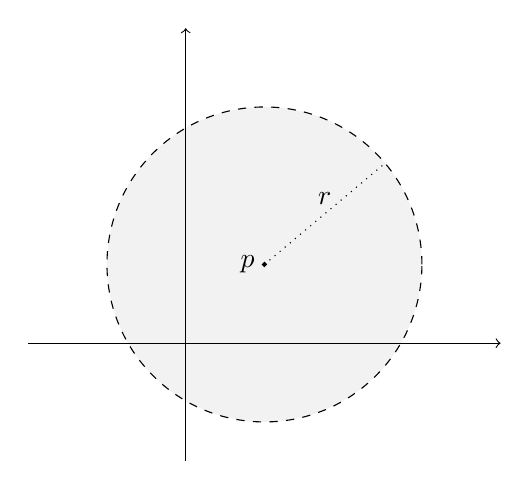
\begin{tikzpicture}
		\draw[dashed,fill=gray!10] (0,0) circle (2);
		\draw[->] (-3,-1) -- (3,-1);
		\draw[->] (-1,-2.5) -- (-1,3);
		\draw (0,0) node[left]{$p$};
		\draw[fill=black] (0,0) circle (.025);
		\draw[dotted] (0,0) to node[anchor=south]{$r$} (40:2);
	\end{tikzpicture}
	\caption{Un intorno $B(\vec p,r)\subset(\R^2,\norm{\cdot})$.}
	\label{fig:B-circ}
\end{figure}

		\item In $(\R^3,\norm{\cdot})$, analogamente al punto precedente, gli intorni sono delle sfere di centro $p$ e raggio $r$, private della superficie sferica.
		\item Con la distanza $d_\infty$, l'intorno $B(\vec 0,r)=\{\vec x\in\R^2\colon\max\{\abs{x_1},\abs{x_2}\}<r\}$ ha la forma di un quadrato di lato $2r$ centrato nell'origine (figura \ref{fig:B-dinfty}).
		\begin{figure}
	\tikzsetnextfilename{intorno-dinfty-r2}
	\centering
	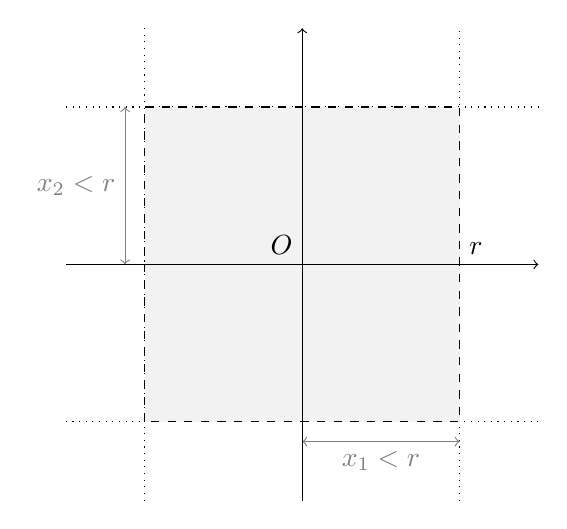
\begin{tikzpicture}
		\draw[dotted] (-3,2) -- (3,2);
		\draw[dotted] (3,-2) -- (-3,-2);
		\draw[dotted] (2,-3) -- (2,0) node[above right]{$r$};
		\draw[dotted] (2,0) -- (2,3);
		\draw[dotted] (-2,-3) -- (-2,3);
		\draw[gray,<->] (-2.25,0) to node[gray,anchor=east]{$\abs{x_2}<r$} (-2.25,2);
		\draw[gray,<->] (0,-2.25) to node[gray,anchor=north]{$\abs{x_1}<r$} (2,-2.25);
		\draw[dashed,fill=gray!10] (-2,-2) rectangle (2,2);
		\draw[->] (-3,0) -- (3,0);
		\draw[->] (0,-3) -- (0,3);
		\draw (0,0) node[anchor=south east]{$O$};
	\end{tikzpicture}
	\caption{Un intorno $B(\vec 0,r)\subset(\R^2,d_\infty)$.}
	\label{fig:B-dinfty}
\end{figure}

		\item Con la distanza $d_1$, l'intorno $B(\vec 0,r)=\{\vec x\in\R^2\colon\abs{x_1}+\abs{x_2}<r\}$ ha la forma di un quadrato ruotato di $\pi/4$, di diagonale $2r$ e centrato nell'origine (figura \ref{fig:B-d1}).
		\begin{figure}
	\tikzsetnextfilename{intorno-d1-r2}
	\centering
	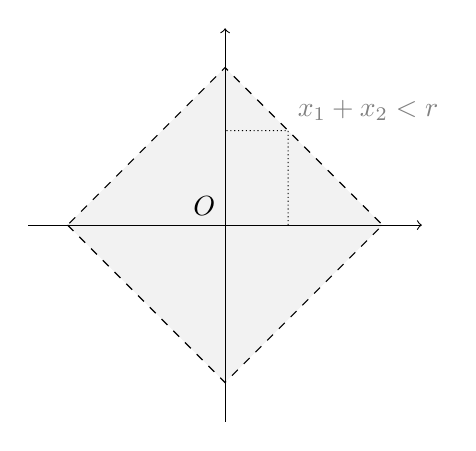
\begin{tikzpicture}
		\filldraw[dashed,fill=gray!10] (-2,0) -- (0,-2) -- (2,0) -- (0,2) -- (-2,0);
		\draw[->] (-2.5,0) -- (2.5,0);
		\draw[->] (0,-2.5) -- (0,2.5);
		\draw[densely dotted] (.8,0) -- (intersection of .8,0--.8,1 and 2,0--0,2) node[gray,anchor=south west]{$\abs{x_1}+\abs{x_2}<r$} -- +(-.8,0);
		\draw (0,0) node[anchor=south east]{$O$};
	\end{tikzpicture}
	\caption{Un intorno $B(\vec 0,r)\subset(\R^2,d_1)$.}
	\label{fig:B-d1}
\end{figure}

		\item Nello spazio $X=\{\phi\colon[a,b]\to\R\colon\phi\text{ è limitata}\}$, con la distanza $d_*$, un intorno di una funzione $f$ è lo spazio limitato dalle funzioni $f-r$ e $f+r$, escluse: $B(f,r)=\{g\in X\colon\sup_{x\in[a,b]}\abs{g(x)-f(x)}<r\}$ (figura \ref{fig:B-d*}).
		\begin{figure}
	\tikzsetnextfilename{intorno-funzione}
	\centering
	\begin{tikzpicture}
		\begin{axis}[standard,xmin=-1,ymin=-1,xmax=7.5,ymax=8,ytick=\empty,xtick={1,6},xticklabels={$a$,$b$},stack plots=y]
			\draw[dotted] (axis cs:1,0) -- (axis cs:1,4.6829);
			\draw[dotted] (axis cs:6,0) -- (axis cs:6,7.4411);
			\draw[gray,<->] (axis cs:3.14,3.14) to node[right]{$r$} (axis cs:3.14,5.14);
			\addplot[draw=none,domain=1:6,samples=200] {-2+x+2*sin(deg(x))};
			\addplot[dashed,domain=1:6,samples=200] {4};
			\addplot[domain=1:6,samples=200] {-2};
			\addplot[dashed,domain=1:6,samples=200] {-2} node[right]{$f-r$};
			\addplot[fill=gray!10,draw=none,domain=1:6,samples=200] {2} node[right]{$f$} \closedcycle;
			\addplot[fill=gray!10,draw=none,dashed,domain=1:6,samples=200] {2} node[right]{$f+r$} \closedcycle;
		\end{axis}
	\end{tikzpicture}
	\caption{Un intorno $B(f,r)\subset(X,d_*)$ della funzione $f=x+2\sin x$.}
	\label{fig:B-d*}
\end{figure}

	\end{enumerate}
\end{esempio}

\begin{teorema}[Proprietà di Hausdorff]
\label{t:hausdorff}
Siano $p$ e $q$ due punti distinti appartenenti ad uno spazio metrico $(X,d)$. Esiste almeno una coppia di raggi $r_1$ e $r_2$ tali che
\[
B(p,r_1)\cap B(q,r_2)=\emptyset.
\]
\end{teorema}
\begin{proof}
	Sia $d$ la distanza tra i due punti $p,q$. Definito $r_1=r_2=\frac{d}3$ le due bolle hanno intersezione vuota. In generale, qualunque coppia di raggi la cui somma sia minore della distanza dei due punti è adatta a dimostrare il teorema.
\end{proof}

\section{Classificazione dei punti}
\begin{definizione}
Siano $(X,d)$ uno spazio metrico e $A\subseteq X$ un suo sottoinsieme. Il punto $p\in X$ si dice
\begin{enumerate}
\item \emph{interno} ad $A$ se esiste una bolla, centrata in $p$, tutta contenuta in tale insieme:
\[
	\exists r>0\colon B(p,r)\subset A;
\]
\item \emph{esterno} ad $A$ se esiste una bolla, centrata in $p$, tutta contenuta nel complementare di tale insieme:
\[
	\exists r>0\colon B(p,r)\subset\compl{A};
\]
\item \emph{di frontiera} se non è interno né esterno, ossia se ogni bolla centrata in $p$ contiene sia punti di $A$ sia del suo complementare:
\[
	\forall r>0,\ B(p,r)\cap A\neq\emptyset\qtext{e}B(p,r)\cap\compl{A}\neq\emptyset.
\]
\end{enumerate}
\end{definizione}
Questa definizione è disgiuntiva ed esaustiva, perché ogni punto rientra sempre in una soltanto delle tre categorie.
L'insieme dei punti interni di $A$ si chiama \emph{interno} e si indica con $\interior{A}$, che non coincide necessariamente con l'insieme stesso. L'insieme dei punti di frontiera, che possono o meno appartenere all'insieme (non si può stabilire a priori) si chiama \emph{frontiera} e si indica con $\boundary A$.
\begin{esempio} \label{es:punti-interni-esterni}
	Applichiamo le definizioni appena date a degli esempi importanti.
	\begin{enumerate}
		\item In ogni spazio metrico $(X,d)$, l'insieme $X$ ha solo punti interni.
		\item Ogni punto è esterno ad un insieme vuoto.
		\item L'interno di un intorno coincide \emph{sempre} con l'intorno stesso.
		\item La frontiera di un intorno $B(\vec p,r)\subset\R^2$ è la circonferenza di raggio $r$, centrata in $\vec p$, cioè $\boundary B=\{\vec x\in\R^2\colon\norm{\vec x-\vec p}=r\}$.
		\item La frontiera dello stesso insieme del punto precedente, ma in $\R^3$, quindi il cerchio $\{\vec x\in\R^3\colon(x_1-p_1)^2+(x_2-p_2)^2<r^2,\ x_3=p_3\}\subset\R^3$ è \emph{l'insieme stesso}, e non più la sua circonferenza.
		\item La frontiera di $\Q\subset\R$ è proprio $\R$, perché ogni intorno di un punto razionale contiene infiniti altri punti razionali e irrazionali (gli irrazionali formano il complementare di $\Q$ rispetto ad $\R$). Analogamente, $\R$ è anche la frontiera di $\R\setminus\Q$.
		\item Con la metrica discreta, se $x\in A$, allora $B(x,1)=\{x\}\subseteq A$, mentre se $y\in\compl{A}$ allora $B(y,1)=\{y\}\subseteq\compl{A}$, quindi ogni punto di un insieme è ad esso interno, mentre ogni punto del complementare è esterno. Quindi la frontiera di un insieme è sempre vuota, anche perché qualsiasi intorno di raggio $r\leq 1$ contiene soltanto il punto, che è il centro della bolla, quindi nessun altro punto del'insieme o del complementare.
	\end{enumerate}
\end{esempio}
\begin{osservazione}
Fissati uno spazio metrico $(X,d)$ e un suo sottoinsieme $A$, se un punto $p\in X$ non è esterno a tale insieme, allora ogni bolla centrata in $p$ di qualsiasi raggio non è un sottoinsieme del complementare di $A$, cioè la sua intersezione con $A$ non è mai vuota:
\[
	\forall r>0,\ B(p,r)\not\subset\compl{A},\text{ vale a dire }B(p,r)\cap A\neq\emptyset.
\]
\end{osservazione}
\begin{definizione}
Siano $(X,d)$ uno spazio metrico e $A\subseteq X$ un suo sottoinsieme. Il punto $p\in X$ non esterno ad $A$ si dice
\begin{itemize}
\item \emph{di accumulazione} per $A$, se ogni bolla centrata in $p$ contiene punti di $A$, oltre al centro stesso della bolla:
\[
\forall r>0,\ B(p,r)\cap A\setminus\{p\}\neq\emptyset;
\]
\item \emph{isolato}, se esiste almeno una bolla centrata nel punto che non contiene altri punti dell'insieme, oltre a $p$ stesso:
\[
\exists r>0\colon B(p,r)\cap A=\{p\}.% uguale a {p} o al vuoto?
\]
\end{itemize}
\end{definizione}
L'insieme dei punti di accumulazione di $A$ si chiama \emph{derivato} e si indica con $A'$. Si dimostra inoltre che se l'intorno di un punto di accumulazione contiene almeno un altro punto dell'insieme, ne contiene infiniti.
\begin{teorema}
Siano $(X,d)$ uno spazio metrico e $A\subseteq X$ un suo sottoinsieme. Se $p\in A'$, l'intersezione tra una bolla di qualsiasi raggio e l'insieme $A$ ha cardinalità infinita.
\[
	\forall r>0,\ \card{B(p,r)\cap A}=\infty.
\]
\end{teorema}
\begin{proof}
Si supponga per assurdo che esista un raggio $\tilde{r}$ tale che la bolla centrata in $p$ abbia cardinalità finita, quindi che $\exists\tilde{r}>0\colon B(p,\tilde{r})\cap A=\{x_1,x_2,\dots,x_n\}$. Per ogni punto $x_i$ di questa bolla possiamo individuare la distanza $r_i=d(p,x_i)$ dal centro, per ogni $i=1,2,\dots,n$. Poiché l'insieme di questi raggi $r_i$ è finito (ha precisamente $n$ elementi), l'esistenza del suo minimo è certa. Allora preso un nuovo raggio $r'$ qualunque tale che $r'<\min_{1\leq i\leq n}\{r_i\}$, una nuova bolla centrata in $p$ non conterrà più alcun elemento di $A$, infatti si ha che
\[
B(p,r')\cap A=\{p\},
\]
cioè $p$ è un punto isolato, che è la negazione della tesi. Quindi il teorema è dimostrato.
\end{proof}
\begin{corollario}
In ogni spazio metrico, il derivato di qualsiasi insieme di cardinalità finita è vuoto.
\[
\forall (X,d),\, A\subseteq X,\text{ se $A$ è finito}\then A'=\emptyset.
\]
\end{corollario}
\section{Insiemi aperti, chiusi e limitati}
\begin{definizione}
\label{d:chiuso-se-c-aperto}
Siano $(X,d)$ uno spazio metrico e $A\subseteq X$ un suo sottoinsieme. $A$ si dice
\begin{itemize}
\item \emph{aperto}, se tutti i suoi punti sono interni, quindi $\interior{A}=A$;
\item \emph{chiuso}, se il suo complementare $\compl{A}$ è aperto.
\end{itemize}
\end{definizione}
Questa non è una definizione esaustiva, infatti esistono insiemi che non sono aperti né chiusi. Si dà anche la seguente caratterizzazione, cioè una condizione necessaria e sufficiente.
\begin{teorema}
Siano $(X,d)$ uno spazio metrico e $A\subseteq X$ un suo sottoinsieme. L'insieme $A$ è chiuso se e solo se contiene i suoi punti di accumulazione.
\[
A\text{ è chiuso}\iff A'\subseteq A.
\]
\end{teorema}
\begin{proof}
(i) Se $A$ è chiuso, contiene i suoi punti di accumulazione.
Sia $p\in \compl{A}$, che quindi per ipotesi, dato che $A$ è chiuso, è aperto. Allora esiste una bolla centrata in $p$ tutta contenuta in $\compl{A}$: quindi l'intersezione di tale bolla con l'insieme $A$ deve essere vuota, e $p$ non può essere un punto di accumulazione di $A$.
\[
\exists r>0\colon B(p,r)\subset \compl{A}\qqq B(p,r)\cap A=\emptyset\qqq p\notin A'.
\]
Necessariamente allora i punti di accumulazione devono trovarsi in $A$.

(ii) Se $A$ contiene i suoi punti di accumulazione, è chiuso.
Sia $A'\subseteq A$ e $p$ un qualsiasi punto del complementare. Per ipotesi $p$ non è di accumulazione per $A$, quindi esiste una bolla $B(p,r)$ che non contiene altri punti di $A$ oltre a $p$ stesso. Poiché $p\in \compl{A}$, tale bolla non contiene alcun punto di $A$: allora $B(p,r)\subseteq \compl{A}$, vale a dire $p$ è interno ad $\compl{A}$. Quindi $\compl{A}$ è aperto, a cui segue che $A$ è chiuso.
\end{proof}
\begin{esempio} \label{es:aperti-chiusi}
	Seguono alcuni semplici e comuni esempi per quanto abbiamo appena visto.
	\begin{enumerate}
		\item Ogni intervallo $(a,b)\subset\R$ è aperto, così come $(a,+\infty)$ e $(-\infty,b)$. Analogamente, $[a,b]$, $[a,+\infty)$ e $(-\infty,b]$ sono chiusi. Intervalli del tipo $[a,b)$ non sono aperti né chiusi.
		\item In ogni spazio metrico $(X,d)$, l'insieme $X$ è aperto perché tutti i suoi punti sono interni. Però $X$ è allo stesso tempo anche chiuso, perché contenendo tutti i punti non può che contenere anche quelli di accumulazione di $X'$. Allora $X$ è sia aperto che chiuso, e quindi anche un insieme vuoto è sia aperto che chiuso. 
		\item Ogni intorno è aperto, per definizione, perché tutti i suoi punti sono interni.
		\item In uno spazio metrico discreto, ogni insieme $A\subseteq X$ è aperto, perché ogni suo punto è interno, ma allo stesso tempo tutti i punti sono isolati, quindi $A'=\emptyset$, quindi $A$ (che ovviamente contiene l'insieme vuoto) è anche chiuso.
	\end{enumerate}
\end{esempio}
\begin{teorema} \label{t:unione-intersezione-aperti}
Siano $(X,d)$ uno spazio metrico e $\{A_i\}_{i\in I}$ una famiglia qualunque di sottoinsiemi aperti di tale spazio metrico. Allora
\begin{enumerate}
\item\[
A=\bigcup_{i\in I} A_i\text{ è aperto};
\]
\item se la famiglia è finita, cioè sia $\{A_1,A_2,\dots,A_n\}$, allora
\[
A=\bigcap_{i=1}^n A_i\text{ è aperto}.
\]
\end{enumerate}
\end{teorema}
\begin{proof}
\begin{enumerate}
\item Sia $p$ appartenente ad $A$, l'insieme unione di tutti gli insiemi della famiglia: questo punto deve allora appartenere ad almeno uno degli insiemi della famiglia, cioè $\exists k\colon p\in A_k$. Poiché tutti questi insiemi sono aperti, $p$ è interno a questo insieme $A_k$, quindi esiste una bolla contenuta tutta in questo insieme, la quale allora è anche contenuta nell'insieme unione: $B(p,r)\subset A_k\subset A$.
\item Sia $p$ un punto appartenente ad $A$, l'insieme intersezione degli insiemi appartenenti alla famiglia finita: questo punto deve allora appartenere a ciascuno degli insiemi della famiglia $A_i,\,\forall i$. Ognuno di questi insiemi è aperto, quindi esiste un raggio tale che la bolla centrata in $p$ sia contenuta in ogni insieme, $\exists r_i\colon \forall i\;B(p,r_i)\subset A_i$. Preso $r'=\min\{r_i\}$, la cui esistenza è garantita dal fatto che la famiglia di insiemi è finita, allora la bolla di raggio $r'$ è contenuta in tutti gli insiemi, quindi anche nell'insieme intersezione: $B(p,r')\subset A$.
\end{enumerate}
\end{proof}
In generale, l'intersezione infinita di aperti non è aperta: ad esempio, sia $A_i=(0,1+\frac1{k})$, per $i\in\N$, l'intersezione dà come risultato $\bigcap_{i=1}^{+\infty}A_i=(0,1]$, che non è aperto né chiuso.
Vale anche il seguente teorema, la cui dimostrazione si ricava dal precedente.
\begin{teorema} \label{t:unione-intersezione-chiusi}
Siano $(X,d)$ uno spazio metrico e $\{C_j\}_{j\in J}$ un una famiglia qualunque di sottoinsiemi chiusi di tale spazio metrico. Allora
\begin{enumerate}
\item\[
C=\bigcap_{j\in J} C_j\text{ è chiuso};
\]
\item se la famiglia è finita, cioè sia $\{C_1,C_2,\dots,C_n\}$, allora
\[
C=\bigcup_{j=1}^n C_j\text{ è chiuso}.
\]
\end{enumerate}
\end{teorema}
\begin{proof}
\begin{enumerate}
\item Passando ai complementari dei risultati del teorema precedente, per le formule di De Morgan si ha
\[
	\compl{C}=\compl{\bigg(\bigcap_{j\in J} C_j\bigg)}=\bigcup_{j\in J}\compl{C_j},
\]
che è l'unione di infiniti insiemi aperti, che per il teorema precedente è aperta. Allora $C$ è chiuso, per la definizione \ref{d:chiuso-se-c-aperto}.
\item Analogamente, si ha
\[
	\compl{C}=\compl{\bigg(\bigcup_{j=1}^n C_j\bigg)}=\bigcap_{j=1}^n\compl{C_j},
\]
che è l'intersezione di un numero finito di insiemi aperti, che quindi per il teorema precedente è aperto. Allora $C$ è chiuso, sempre per la \ref{d:chiuso-se-c-aperto}.\qedhere
\end{enumerate}
\end{proof}
Analogamente al controesempio precedente, l'unione di infiniti chiusi non è sempre chiusa: se $C_j=[0,1-\frac1{k}]$ con $j\in\N$, si ha che $\bigcup_{j=1}^{+\infty}C_j=[0,1)$ che non è chiuso, e nemmeno aperto.
\begin{definizione}
Siano $(X,d)$ uno spazio metrico e $A\subseteq X$ un suo sottoinsieme. Si chiama \emph{chiusura} di $A$, e si indica con $\clos{A}$, il più piccolo insieme chiuso che lo contiene. Questo insieme coincide con l'unione dell'insieme stesso con il suo derivato.
\[
\clos{A}=A\cup A'.
\]
\end{definizione}
Si dimostrano che:
\begin{teorema}
Siano $(X,d)$ uno spazio metrico e $A\subseteq X$ un suo sottoinsieme. 
\begin{enumerate}
\item $\clos{A}$ è sempre chiuso;
\item se $F$ è chiuso e $A\subseteq F$, allora $\clos{A}\subseteq F$;
\item se $A$ è chiuso, $\clos{A}=A$ (perché, semplicemente, $A'=A$).
\end{enumerate}
\end{teorema}
\begin{definizione}
Un insieme è \emph{limitato} se esiste, finito, l'estremo superiore delle distanze reciproche tra tutti i suoi elementi.
\[
\sup_{x,y\in A} d(x,y)<+\infty.
\]
Tale estremo superiore è detto \emph{diametro} dell'insieme.
\end{definizione}
Se $A\subseteq (X,d)$ è un insieme limitato, allora il suo diametro coincide con quello della sua chiusura: $\diam A=\diam\clos{A}$; inoltre $\exists p\in X$ e $r>0$ tali per cui $A\subset B(p,r)$, ossia un insieme limitato può essere sempre contenuto in una bolla di opportuno raggio.
\begin{esempio} \label{es:insiemi-limitati}
	Alcuni insiemi limitati e i loro diametri:
	\begin{enumerate}
		\item se $A\subset\R$ un insieme limitato, non vuoto, il suo diametro è dato da $\sup A-\inf A$;
		\item con la metrica discreta il diametro di qualsiasi insieme di almeno due punti è sempre 1, quindi ogni insieme è limitato.
	\end{enumerate}
\end{esempio}

\chapter{Successioni}
\section{Introduzione}
Le successioni sono famiglie di elementi del tipo $\{a_n\}_{n=1}^{\infty}$, con $a_n\in (X,d)$ e $\forall n\in\N$, e sono propriamente definite come funzioni dell'insieme dei naturali su uno spazio metrico.
\[
f\colon\N\to (X,d).
\]
L'immagine $f(n)$, con $n$ sempre naturale, viene indicata con $a_n$, che si chiama \emph{termine generale} della successione, che invece si indica, tra i vari modi, con $\{a_n\}$, che indica anche il suo codominio, ossia l'insieme delle immagini $a_n$.
Si può descrivere una successione, quindi, anche con l'espressione
\[
f\colon n\to f(n)=a_n.
\]
\begin{definizione}
Si dice che una definizione soddisfa una proprietà \emph{definitivamente} se tale proprietà è vera per $n$ sufficientemente grande, cioè se esiste un valore $N$ tale che per ogni $n>N$ il termine $a_n$ verifica la proprietà.
\end{definizione}
È diverso affermare che una successione verifica una proprietà per infiniti $n$ o definitivamente: quest'ultimo modo si usa per dire che, per \emph{tutti} gli $n$ maggiori di un certo numero $N$, la proprietà è verificata. Ad esempio, la successione a valori reali $a_n=(-1)^n$ soddisfa la proprietà $a_n=1$ per infiniti $n$, ma non definitivamente, infatti continua ad oscillare tra 1 e $-1$ e non si può stabilire un numero $n=N$ oltre il quale $a_n$ verifichi \textit{sempre} la proprietà.

\section{Successioni convergenti}
\begin{definizione}
Siano $\{a_n\}\subset(X,d)$ e $\ell\in X$. Si dice che la successione $\{a_n\}$ \emph{converge} a $\ell$ se per ogni numero $\epsilon$ arbitrariamente piccolo $\{a_n\}$ verifica definitivamente la proprietà $d(a_n,\ell)<\epsilon$, oppure equivalentemente che, sempre definitivamente, $a_n\in B(\ell,\epsilon)$.
\[
\forall\epsilon >0\;\exists N\colon\forall n\geq N\to d(a_n,\ell)<\epsilon.
\]
\end{definizione}
\begin{definizione}
Il numero $\ell\in X$ si chiama \emph{limite} della successione $\{a_n\}\subset(X,d)$ se
\[
\lim_{n\to +\infty}a_n=\ell.
\]
\end{definizione}
\begin{teorema}
\label{t:succ_limitata}
Se la successione $\{a_n\}$ a valori nello spazio metrico $(X,d)$ è convergente, allora è limitata.
\end{teorema}
\begin{proof}
Si scelga $\epsilon=1$ come raggio dell'intorno. Sia $\ell$ il limite della successione: per ipotesi, esiste un numero intero $N$ tale che $\forall n\geq N$ risulta $a_n\in B(\ell,1)$. Allora l'insieme formato dai valori di $\{a_n\}$ per $n\geq N$ ha un diametro inferiore o uguale a 2, quindi è limitata. Allora poiché l'insieme dei valori della successione per $n<N$ è di cardinalità finita, è limitato anch'esso, quindi tutta la successione è limitata in quanto somma di due insiemi limitati.
\end{proof}
Una successione è limitata quando il suo codominio è limitato, ma questo non implica necessariamente che la successione converga ad un limite. Come esempio si può considerare, come prima, la successione $a_n=(-1)^n$ che è chiaramente limitata, ma non converge.
\begin{teorema}[di unicità del limite] \label{t:unicita_limite}
Siano $\{a_n\}\subset(X,d)$ e $\ell_1,\ell_2\in X$. Se $a_n\to\ell_1$ e $a_n\to\ell_2$ allora $\ell_1=\ell_2$, vale a dire che una successione, se converge, non può convergere a due limiti differenti.
\end{teorema}
\begin{proof}
Sia per assurdo $\ell_1\neq\ell_2$. Deve allora esistere una distanza non nulla tra di loro. Si considerino allora due raggi $r_1$ e $r_2$ tali che $r_1+r_2\leq d(\ell_1,\ell_2)$: per il teorema di Hausdorff \ref{t:hausdorff} questi due raggi individuano rispettivamente gli intorni $B(\ell_1,r_1)$ e $B(\ell_2,r_2)$, tali che $B(\ell_1,r_1)\cap B(\ell_2,r_2)=\emptyset$. Perché la successione converga ad entrambi i limiti, deve essere definitivamente contenuta in entrambi gli intorni, ma ciò è assurdo, quindi i due limiti $\ell_1$ e $\ell_2$ devono coincidere.
\end{proof}

\section{Successioni a valori reali}
Si identificano con questa definizione tutte le successioni le cui immagini sono numeri reali, ossia
\[
f\colon\N\to\R.
\]
La definizione di limite in questo caso si può riscrivere affermando che se la successione converge a $\ell$, è definitivamente contenuta nell'intervallo $(\ell-\epsilon,\ell+\epsilon)$, perché $|a_n-\ell|<\epsilon$.
Per il teorema \ref{t:succ_limitata} allora ogni successione convergente è sia superiormente che inferiormente limitata.

\begin{definizione}
Una successione si dice \emph{divergente} all'infinito se i suoi elementi, in valore assoluto, sono definitivamente grandi. In particolare:
\begin{itemize}
\item $a_n\to +\infty$ se $\forall M>0\;\exists N\colon\forall n\geq N\to a_n>M$;
\item $a_n\to -\infty$ se $\forall M>0\;\exists N\colon\forall n\geq N\to a_n<-M$.
\end{itemize}
\end{definizione}
\begin{teorema}
Se la successione $\{a_n\}$ diverge a $+\infty$, allora non è limitata superiormente. Analogamente, se $a_n\to -\infty$ non è limitata inferiormente.
\end{teorema}
Non è però sempre valido il contrario, cioè una successione illimitata superiormente non è necessariamente divergente a $+\infty$. Come esempio si consideri la successione
\[
a_n=
\begin{cases*}
	n & se $n$ è pari\\
	1 & se $n$ è dispari
\end{cases*}.
\]
Ovviamente questa successione non è limitata, ma non è verificato \emph{definitivamente} che sia arbitrariamente grande.
\begin{teorema}[di permanenza del segno]
\label{t:permanenza_segno}
Sia $\{a_n\}$ una successione a valori reali convergente ad $a$.
\begin{enumerate}
\item Se $a$ è positivo, allora gli elementi della successione sono definitivamente positivi.
\item Se la successione è definitivamente positiva, allora $a\geq 0$.
\end{enumerate}
\end{teorema}
\begin{proof}
Se la successione converge ad un valore $a$ positivo, scelto un $\epsilon>0$, arbitrariamente piccolo,  deve essere che $a-\epsilon>0$. Poiché $a$ è il limite della successione, i suoi elementi sono definitivamente compresi nell'intorno $(a-\epsilon,a+\epsilon)$, ossia sono sicuramente maggiori di $a-\epsilon$. Dato che $a-\epsilon$ è positivo, segue che anche gli $a_n$ devono essere definitivamente positivi.

Sia ora definitivamente $a_n>0$. Se il suo limite $a$ fosse negativo, per il punto precedente la successione dovrebbe essere definitivamente negativa, che è assurdo: quindi il suo limite non è negativo.
\end{proof}
Analogamente si dimostra che se $\{a_n\}$ converge ad un valore $a<0$, i suoi elementi sono definitivamente negativi, e che se una successione è convergente e definitivamente negativa, il suo limite è negativo o nullo.
La seconda parte del teorema \emph{non è l'inverso} della prima, in quanto anche se la successione è definitivamente positiva il limite non è sempre positivo, ma può essere anche nullo, come per la successione di $1/n$, chiaramente sempre positiva ma convergente a 0.
Questo teorema può essere ``traslato'' sostituendo 0 con un altro numero e verificando che la successione converga ad un valore maggiore di quel numero.
Questi ultimi due teoremi suppongono che il limite della successione esista, infatti la convergenza della successione è un'ipotesi fondamentale.
\begin{teorema}[del confronto]
\label{t:confronto}
\begin{enumerate}
\item Siano $\{a_n\}$, $\{b_n\}$ e $\{c_n\}$ tre successioni a valori reali, con $a_n\leq b_n\leq c_n$ definitivamente. Se le successioni $a_n$ e $c_n$ convergono entrambe ad un limite $\alpha$, allora $b_n$ ammette il limite, e tale limite coincide con $\alpha$.
\item Siano $\{a_n\}$ e $\{b_n\}$ due successioni a valori reali, con $a_n\leq b_n$ definitivamente:
	\begin{itemize}
		\item se $a_n$ diverge a $+\infty$, allora anche $b_n$ ammette il limite, che è $+\infty$;
		\item se $b_n$ diverge a $-\infty$, allora anche $a_n$ ammette il limite, che è $-\infty$.
	\end{itemize}
\end{enumerate}
\end{teorema}
\begin{proof}
\begin{enumerate}
\item Per la convergenza di $a_n$ e $c_n$ si ha che
	\begin{itemize}
		\item $\forall\epsilon>0\;\exists N_1\colon\forall n\geq N_1\to\alpha-\epsilon<a_n<\alpha+\epsilon$;
		\item $\forall\epsilon>0\;\exists N_2\colon\forall n\geq N_2\to\alpha-\epsilon<c_n<\alpha+\epsilon$.
	\end{itemize}
Per tutti gli $n\geq\max\{N_1,N_2\}$ devono sussistere entrambe le proprietà. Allora, poiché per ipotesi $b_n$ è compreso tra le altre due successioni, risulta
\[
\alpha-\epsilon<a_n\leq b_n\leq c_n<\alpha+\epsilon,
\]
A questa relazione segue che $\alpha-\epsilon<b_n<\alpha+\epsilon$, che significa che anche $b_n$ converge ad $\alpha$.
\item Nel caso in cui $a_n\to +\infty$, segue che definitivamente $a_n>M$ con $M$ arbitrariamente grande. Poiché è, per ipotesi, $b_n\geq a_n$, allora definitivamente si ha $b_n\geq a_n>M$, quindi $b_n>M$, cioè diverge a $+\infty$.
Analogamente si dimostra il caso in cui $b_n\to -\infty$.\qedhere
\end{enumerate}
\end{proof}
Nel teorema del confronto non è nota a priori l'esistenza dei limiti delle successioni che sono dimostrate come convergenti o divergenti, quindi è possibile utilizzare questo teorema per dimostrare l'esistenza di tali limiti.
Dal teorema del confronto segue che
\begin{osservazione}
Sia $\{a_n\}$ il prodotto di due successioni $b_n$ e $c_n$. Se $b_n\to 0$ e $c_n$ è limitata, la successione $a_n=b_n\cdot c_n$ converge a 0.
\end{osservazione}

\begin{definizione}
Sia $\{a_n\}$ una successione convergente a valori reali. Si dice che $a_n$ tende a $\ell\in\R$ per \emph{eccesso} (e si indica $a_n\to\ell^+$) se la successione è definitivamente compresa nell'intorno destro di $\ell$, cioè in $[\ell,\ell+\epsilon)$.
Analogamente, $a_n$ tende a $\ell\in\R$ per \emph{difetto} (e si indica $a_n\to\ell^-$) se la successione è definitivamente compresa nell'intorno sinistro di $\ell$, cioè in $(\ell-\epsilon,\ell]$.
\end{definizione}

\section{Calcolo dei limiti}
\subsection{Algebra parziale di $\Rex$}
Si può estendere l'insieme dei numeri reali per comprendere anche il concetto di infinito, negativo e positivo, ottenendo l'insieme dei numeri reali \emph{esteso} $\Rex=\R\cup\{-\infty\}\cup\{+\infty\}$. In questo insieme valgono ovviamente tutte le proprietà di somma e prodotto quando $a$ e $b$ sono finiti, ma non valgono più tutte se uno dei due è $\pm\infty$, infatti $\Rex$ non è più un campo.

\begin{teorema}
Siano $\{a_n\}$ e $\{b_n\}$ due successioni a valori reali, e sia $a_n\to a$ e $b_n\to b$, con $a,b\in\Rex$. Allora
\begin{itemize}
	\item la successione $a_n+b_n$ ammette limite, e tale limite è $a+b$, purché la somma $a+b$ sia definita in $\Rex$;
	\item la successione $a_nb_n$ ammette limite, e tale limite è $ab$, purché il prodotto $ab$ sia definito in $\Rex$.
\end{itemize}
\end{teorema}
Nei casi non compresi da questo teorema, il risultato dell'operazione tra i due limiti non è definito, e si ha una \emph{forma di indecisione}, e in questi casi il risultato non si può sapere a priori, deducendolo da teoremi o formule note, ma bisogna calcolarlo caso per caso, in quanto non è mai stabilito. Le forme di indecisione si presentano nelle seguenti forme:
\begin{gather*}
\infty-\infty\qquad 0\cdot\infty\qquad\frac{\infty}{\infty}\\
\frac00\qquad 1^\infty\qquad 0^0\qquad \infty^0
\end{gather*}
Inoltre, si possono applicare alle successioni alcune funzioni elementari, come il logaritmo o le funzioni trigonometriche, e il limite della funzione si può calcolare come la funzione del limite della successione, come afferma il seguente teorema.
\begin{teorema}
Sia $\{a_n\}$ una successione a valori reali convergente al numero $a$. Sia $f\colon D\subseteq\R\to\R$ una funzione ``elementare''. Se la successione $a_n$ e il suo limite $a$ appartengono a $D$, allora
\[
f(a_n)\to f(a).
\]
\end{teorema}

\paragraph{Confronto di infiniti}
Per calcolare più velocemente il rapporto di due successioni divergenti si stabilisce quale tipo di funzione ``diverge più velocemente'', confrontando i tipi di infiniti. Si definisce così una scala di tipi di successioni, ordinate partendo dalla più lenta a divergere:
\[
\log_a^b n\qquad n^c\qquad d^n\qquad n!\qquad n^n,
\]
con i vari coefficienti scelti opportumanente in modo che le successioni divergano. Il rapporto di uno di questi infiniti per uno qualsiasi dei precedenti tende a infinito, con il segno opportuno, e ovviamente il reciproco tende a zero.

\section{Successioni monotone}
Sia $\{a_n\}$ una successione a valori reali. Si dice che la successione è monotona:
\begin{itemize}
\item crescente in senso stretto, se $\forall n$ si ha $a_n<a_{n+1}$;
\item crescente in senso lato, se $\forall n$ si ha $a_n\leq a_{n+1}$;
\item decrescente in senso stretto, se $\forall n$ si ha $a_n>a_{n+1}$;
\item decrescente in senso lato, se $\forall n$ si ha $a_n\geq a_{n+1}$.
\end{itemize}
Si può eventualmente definire una successione come \emph{definitivamente monotona}, quando vale una delle quattro relazioni precedenti ma solo per tutti i valori di $n$ oltre un certo numero $N$. Le proprietà delle successioni monotone valgono in entrambi i casi, con le opportune modifiche del caso, ossia di ignorare nei calcoli la parte della successione per $n<N$.

Il seguente teorema garantisce l'esistenza del limite per tali successioni.
\begin{teorema}
Tutte le successioni monotone sono regolari. Sia inoltre $\{a_n\}$ una successione a valori reali: se è monotona crescente, allora
\[
\lim_{n\to +\infty} a_n=\sup\{a_n\},
\]
e tale limite è finito se la successione è limitata, altrimenti è $+\infty$.
Se $\{a_n\}$ è invece monotona decrescente, allora
\[
\lim_{n\to +\infty} a_n=\inf\{a_n\},
\]
e tale limite è finito se la successione è limitata, altrimenti è $-\infty$.
\end{teorema}
\begin{proof}
Si supponga $\{a_n\}$ monotona crescente, e sia $\sup\{a_n\}=\ell\in\R$. Allora $\ell$ è un maggiorante, e anche il minimo dei maggioranti. Quindi
\[
a_n\leq\ell\;\forall n\text{ e }\forall\epsilon>0\;\exists N\colon\ell-\epsilon<a_N\leq\ell.
\]
L'elemento $a_{N+1}$ deve essere maggiore di $a_N$, perché la successione è crescente, e al contempo deve essere minore di $\ell$, e così via per ogni elemento di $a_n$ che segue nell'ordinamento della successione. Tutti gli elementi $a_n$ sono tali che, $\forall n>N$:
\[
\ell-\epsilon<a_N\leq a_n\leq\ell,
\]
quindi appartengono all'intorno sinistro di $\ell$, cioè $a_n\to\ell^-$ per $n\to +\infty$.

Sia ora $\sup\{a_n\}=+\infty$. Poiché non ci sono maggioranti, vale che $\forall M>0$ $\exists a_N>M$, e dato che la successione è crescente, esiste $N\colon\forall n\geq N$ si ha che $a_n\geq a_N>M$, quindi $a_n\to +\infty$ per $n\to +\infty$.

La dimostrazione per $\{a_n\}$ decrescente è analoga.
\end{proof}
Tra le successioni monotone crescenti ne esiste una molto particolare, che definisce il numero $e$. Si definisce infatti la successione
\[
e_n\equiv\left(1+\frac1{n}\right)^n,
\]
per cui vale il teorema seguente.
\begin{teorema}
La successione $e_n$ è strettamente monotona crescente e superiormente limitata. Essa ammette quindi un limite finito, e tale limite è il numero $e$.
\[
\lim_{n\to +\infty} e_n=\sup\{e_n\}=e.
\]
\end{teorema}
Tale numero è trascendente in quanto non è mai radice di un polinomio a coefficienti razionali. Una prima approssimazione del numero è
\[
e\approx\num{2.718281828459}.
\]
A partire da questo si definiscono i logaritmi, così come le potenze, in base $e$. Valgono inoltre i seguenti limiti notevoli:
\begin{gather*}
(1+a\epsilon_n)^{1/\epsilon_n}\to e^a;\qquad\qquad\frac{\log(1+\epsilon_n)}{\epsilon_n}\to 1;\\
\frac{e^{\epsilon_n}-1}{\epsilon_n}\to 1;\qquad\qquad\frac{(1+\epsilon_n)^b-1}{\epsilon_n}\to b.
\end{gather*}
\begin{proof}
Il primo non è altro che la successione $e_n$ riscritta diversamente per una successione infinitesima generica. Da questa si dimostrano:
\begin{itemize}
\item Applicando i logaritmi a $(1+\epsilon_n)^{1/\epsilon_n}\to\epsilon_n$ si ottiene che
\[
\log(1+\epsilon_n)^{1/\epsilon_n}\to\log e\text{,  da cui  }\frac{\log(1+\epsilon_n)}{\epsilon_n}\to 1.
\]
\item Sia $x_n\equiv e^{\epsilon_n}-1$, che quindi è infinitesima. Allora $e^{\epsilon_n}=x_n+1$, e applicando i logaritmi si ha $\epsilon_n=\log(x_n+1)$, quindi
\[
\frac{e^{\epsilon_n}-1}{\epsilon_n}=\frac{x_n}{\log(1+x_n)}\to 1.
\]
\item Sia $y_n\equiv a\log(1+\epsilon_n)$, che è infinitesima. Applicando la potenza in base $e$ si trova che $e^{y_n}=e^{a\log(1+\epsilon_n)}=(1+\epsilon_n)^a$, quindi
\[
\frac{(1+\epsilon_n)^a-1}{\epsilon_n}=\frac{e^{y_n}-1}{y_n}\cdot\frac{y_n}{\epsilon_n}=\frac{e^{y_n}-1}{y_n}\cdot\frac{a\log(1+\epsilon_n)}{\epsilon_n}\to a.\qedhere
\]
\end{itemize}
\end{proof}

\section{Infiniti e infinitesimi}
Una successione si dice infinitesima de tende a zero, mentre è infinita se diverge. Esistono due utili criteri per stabilire se una successione è uno di questi due tipi.

\begin{teorema}[Criterio del rapporto]
\label{t:criterio_del_rapporto_successioni}
Sia $\{a_n\}$ una successione a valori reali definitivamente positivi. Se esiste il limite del rapporto,
\[
\lim_{n\to +\infty} \frac{a_{n+1}}{a_n}\equiv\alpha,
\]
con $\alpha\in\Rex$ (è anche positivo, poiché i due termini della frazione sono positivi), allora:
\begin{itemize}
	\item se $\alpha<1$, $a_n$ converge a 0;
	\item se $\alpha>1$, $a_n$ diverge a $+\infty$.
\end{itemize}
\end{teorema}
Questo teorema inoltre garantisce l'esistenza del limite della successione. Il caso in cui $\alpha=1$ non è preso in considerazione in quanto è di indecisione, e non non si può dire niente sul comportamento della successione.
\begin{proof}
1) Sia $\alpha<1$: allora, dato un numero $\epsilon>0$ arbitrariamente piccolo per cui $\alpha+\epsilon<1$, esiste $N$ tale che per ogni $n>N$ si abbia $\alpha-\epsilon<a_{n+1}/a_n<\alpha+\epsilon$, perché per la definizione di limite la successione $a_{n+1}/a_n$ è definitivamente contenuta in un arbitrario intorno di $\alpha$. Allora, per questi valori di $n$, la successione $a_n$ si può scrivere come
\[
a_n=\frac{a_n}{a_{n-1}}\cdot a_n=\frac{a_n}{a_{n-1}}\cdot\frac{a_{n-1}}{a_{n-2}}\cdot\frac{a_{n-2}}{a_{n-3}}\dots \frac{a_{N+1}}{a_N}\cdot a_N.
\]
Tutti i rapporti di questo tipo, cioè $a_k/a_{k-1}$, sono per $n>N$ minori di $\alpha+\epsilon$, quindi
\[
\begin{split}
	a_n&<(\alpha+\epsilon)(\alpha+\epsilon)\cdots(\alpha+\epsilon)a_N\\
	&=(\alpha+\epsilon)^{n-N}a_N\\
	&=\frac{a_N}{(\alpha+\epsilon)^N}\cdot (\alpha+\epsilon)^n,
\end{split}
\]
dove il termine $a_N/(\alpha+\epsilon)^N$ è un numero, costante, mentre $(\alpha+\epsilon)^n$ è una successione convergente a 0. Dato che
\[
0<a_n<\frac{a_N}{(\alpha+\epsilon)^N}\cdot (\alpha+\epsilon)^n,
\]
si ha che per il teorema \ref{t:confronto} del confronto anche $a_n\to 0$.

2) Sia $\alpha>1$, e analogamente al caso precedente si consideri $\epsilon>0$ tale che $\alpha-\epsilon>1$; allora si ha che, definitivamente, $\alpha-\epsilon<a_{n+1}/a_n<\alpha+\epsilon$, quindi $\exists\tilde{N}$ per cui $\forall n>\tilde{N}$ tutte le frazioni del tipo $a_k/a_{k-1}$ sono maggiori di $\alpha-\epsilon$. Allora, riscrivendo la successione $a_n$ come nel caso precedente, si ha che
\[
a_n>(\alpha-\epsilon)^n\cdot\frac{a_N}{(\alpha-\epsilon)^N},
\]
a cui segue, sempre per il teorema \ref{t:confronto}, che $a_n\to +\infty$.
\end{proof}
\begin{teorema}[Criterio della radice]
\label{t:criterio_della_radice_successioni}
Sia $\{a_n\}$ una successione a valori reali definitivamente positivi. Se esiste il limite del rapporto,
\[
\lim_{n\to +\infty} \sqrt[n]{a_n}\equiv\alpha,
\]
con $\alpha\in\Rex$ (è anche positivo, dato che l'argomento della radice è positivo), allora:
\begin{itemize}
	\item se $\alpha<1$, $a_n$ converge a 0;
	\item se $\alpha>1$, $a_n$ diverge a $+\infty$.
\end{itemize}
\end{teorema}
La dimostrazione è simile a quella del teorema precedente.

Grazie a questi teoremi è possibile dimostrare alcuni dei confronti tra infiniti:
\begin{enumerate}
\item Sia $x_n\equiv\dfrac{a^n}{n^b}$, con $a>1$ e $b>0$. La successione $x_{n+1}/x_n$ è
\[
\frac{x_n}{x_{n+1}}=\frac{a^{n+1}}{a^n}\cdot\frac{n^b}{(n+1)^b}=a\cdot\frac{(n+1-1)^b}{(n+1)^b}=a\,\left(1-\frac{1}{n+1}\right)^b\to a.
\]
Per il criterio del rapporto, poiché $a>1$ allora $x_n\to +\infty$, cioè $\dfrac{a^n}{n^b}\to +\infty$.
\item Sia $y_n\equiv\dfrac{n!}{a^n}$, con $a>1$. La successione $y_{n+1}/y_n$ è
\[
\frac{y_n}{y_{n+1}}=\frac{(n+1)!}{a^{n+1}}\cdot\frac{a^n}{n!}=\frac{n+1}{a}>1.
\]
Quindi $y_n\to +\infty$ per il criterio del rapporto.
\end{enumerate}

\section{Successioni asintotiche}
Spesso, per studiare l'andamento di una successione al limite, è utile poterla approssimare e quindi sostituire con una più semplice. Questo è possibile con la seguente definizione.
\begin{definizione}
\label{d:asintotico}
Due successioni $\{x_n\}$ e $\{y_n\}$ si dicono \emph{asintotiche}, e si scrive $x_n\sim y_n$, se il loro rapporto tende a 1.
\[
\lim_{n\to +\infty}\frac{x_n}{y_n}=1.
\]
\end{definizione}
La relazione $\sim$ è riflessiva, simmetrica e transitiva.
\begin{definizione}
Date due successioni $\{x_n\}$ e $\{y_n\}$, si dice che $x_n$ è \emph{o-piccolo} di $y_n$, e si scrive $x_n=o(y_n)$, se il loro rapporto è infinitesimo:
\[
\lim_{n\to +\infty}\frac{x_n}{y_n}=0.
\]
\end{definizione}
La scrittura $o(1)$ indica un infinitesimo generico.
Il limite del rapporto della \ref{d:asintotico} può essere riscritto usando questa notazione, cioè se $a_n\sim\alpha b_n$ allora $a_n=\alpha b_n+o(b_n)$. Infatti dividendo l'ultima relazione per $b_n$ si ha che
\[
\frac{a_n}{b_n}=\frac{\alpha b_n}{b_n}+\frac{o(b_n)}{b_n}=\alpha+o(1)\text{, cioè }\frac{a_n}{b_n}\to\alpha.
\]
Da ciò si può notare come la scrittura con gli o-piccoli mostra l'errore che si commette approssimando una successione con l'altra, cosa che non accade sfruttando l'uguaglianza asintotica, che è infatti è ``sicura'' da utilizzare soltanto in caso di prodotti e altri casi particolari.
Si noti inoltre che la scrittura, ad esempio, $e^{\epsilon_n}\sim 1+\epsilon_n$, per quanto corretta dal punto di vista delle relazioni, non ha molto senso: infatti, dato che l'uguaglianza asintotica è ``interessata'' soltanto dai termini di ordine maggiore, da quella relazione segue che $e^{\epsilon_n}\sim 1$, che per quanto vera non dà alcuna informazione utile. È invece corretta la scrittura $e^{\epsilon_n}=1+\epsilon_n+o(\epsilon_n)$.

\section{Condizione di Cauchy}
Senza bisogno di calcolare il limite, esistono dei teoremi che permettono di garantire la convergenza di una successione. La condizione di Cauchy, ad esempio, non fa alcun riferimento al valore del limite, ma considera la distanza tra due elementi della successione.
\begin{definizione}[condizione di Cauchy]
\label{d:ccauchy_successioni}
Sia $\{x_n\}$ una successione a valori in uno spazio metrico $(X,d)$. Si dice che la successione soddisfa la condizione di Cauchy se $\forall\epsilon>0$ vale
\begin{equation}
\label{eq:ccauchy_successioni}
\exists N\colon\forall m,n>N\text{ si ha che }d(x_m,x_n)<\epsilon,
\end{equation}
ossia se la distanza tra due generici elementi della successione è definitivamente infinitesima.
\end{definizione}
\begin{osservazione}
Se una successione converge, soddisfa necessariamente la condizione di Cauchy.
\end{osservazione}
\begin{proof}
Sia $\{x_n\}$ una successione convergente a $p$. Per la distanza triangolare, presi due elementi $x_n$ e $x_m$ della successione, si ha
\[
d(x_n,x_m)\leq d(x_n,p)+d(x_m,p).
\]
Il secondo membro della disuguaglianza, per la definizione di limite, è arbitrariamente piccolo, perciò lo è anche la distanza $d(x_n,x_m)$, quindi la condizione di Cauchy è soddisfatta.
\end{proof}
Questo non significa però che una successione che soddisfa la condizione di Cauchy sia anche convergente: non vale insomma il teorema inverso.
\begin{osservazione}
Ogni successione che soddisfa la condizione di Cauchy è limitata.
\end{osservazione}
\begin{proof}
Sia $\epsilon=1$, allora per la condizione di Cauchy $\exists N\colon\forall n\geq N$ si ha $d(x_n,x_m)<1$. Quindi per $n\geq N$ si ha che $x_n\in B(x_N,1)$. Al di fuori dell'intorno rimangono al più un numero finito di elementi (tutti quelli per cui $n<N$): sia $r_i=d(x_N,x_i)$ con $i=1,2,\dots,N-1$, preso un qualunque $R>\max\{r_i\}$ allora tutta la successione $\{x_n\}$ è compresa in $B(x_N,R)$, perciò è limitata.
\end{proof}
La successione di Cauchy quindi implica la limitatezza della successione, ma non è ancora sufficiente per determinarne la convergenza. Questa proprietà infatti dipende dallo spazio metrico in cui è posta la successione.
\paragraph{Esempi}
\begin{itemize}
\item Nello spazio metrico $(\Q,\abs{\cdot})$, una successione qualsiasi convergente a $\sqrt{2}$, come ad esempio quella dei troncamenti degli allineamenti decimali che la approssimano, soddisfa la condizione di Cauchy, in quanto converge in $\R$ dato che la metrica è la stessa per entrambi gli spazi metrici. Tuttavia il limite di tale successione non appartiene a $\Q$, perciò non converge.
\item Si definisca per ogni $m,n\in\N$ la distanza $d^*(n,m)=\abs{\dfrac1{n}-\dfrac1{m}}$. Si può dimostrare che $(\N,d^*)$ è uno spazio metrico. La successione $x_n=n$ soddisfa la condizione di Cauchy, poiché
\[
\abs{\frac1{n}-\frac1{m}}\leq\frac1{n}+\frac1{m}<\epsilon
\]
se vale $m,n>1/2\epsilon$. Tuttavia la successione non converge, infatti supposto che converga al limite $k\in\N$, si ha
\[
\lim_{n\to +\infty} d^*(x_n,k)=\abs{\frac1{k}-\frac1{n}}=\frac1{k}\neq 0.
\]
\end{itemize}
Esistono però alcuni spazi metrici in cui ogni successione che soddisfa la condizione di Cauchy è anche convergente.
\begin{definizione}
Uno spazio metrico si dice \emph{completo} se in esso ogni successione che verifica la condizione di Cauchy è anche convergente.
\end{definizione}
Gli spazi $(\Q,\abs{\cdot})$ e $(\N,d^*)$ non sono quindi completi, per i controesempi precedenti. Gli spazi $(\R^n,\norm{\cdot})$ invece lo sono, come dimostrato di seguito.
\begin{lemma}
Sia $\{I_n\}_{n=1}^{\infty}$ una successione di intervalli chiusi, con $I_{n+1}\subseteq I_n$ $\forall n$. Allora
\[
\bigcap_{n=1}^{\infty} I_n\neq\emptyset.
\]
Inoltre, se $\diam\{I_n\}\to 0$, allora $\bigcap_{n=1}^{\infty} I_n$ è un punto isolato (la sua cardinalità è 1).
\end{lemma}
\begin{proof}
Gli intervalli $I_n$ sono della forma $[a_n,b_n]$, con opportuni $a_n\leq b_n$. Per la relazione di inclusione, gli $a_n$ formano una successione monotona crescente, mentre $b_n$ è monotona decrescente. Inoltre, entrambe sono limitate perché $a_n\leq b_1$ e $b_n\geq a_1$, quindi entrambe ammettono limite, rispettivamente
\[
\lim_{n\to+\infty}a_n=\sup a_n\equiv A\qtext{e}\lim_{n\to+\infty}b_n=\inf b_n\equiv B.
\]
Sia ora per assurdo che $B<A$, che quindi individuano l'intervallo $[B,A]$. Allora per i limiti precedenti $\exists N\colon\forall n\geq N$ $a_n\in[B,A]$ e $\exists M\colon\forall n\geq M$ $b_n\in[B,A]$. Quindi se si prende $K\geq\max\{N,M\}$, poiché per ipotesi $a_n<b_n$, si avrà che $B<a_K<b_K<A$. Ma proseguendo con gli indici, per $H>K$ si avrà $B<b_H<a_K<A$, che contrasta con l'ipotesi per cui $a_n\leq b_n$ per ogni $n\in\N$. Allora deve essere $A\leq B$, quindi l'intervallo $[A,B]$ è contenuto nell'intersezione di tutti gli $I_n$. Se infine $a_n$ e $b_n$ tendono ad un unico limite $p$, allora l'intervallo si riduce a $[A,B]\to p$, quindi l'intersezione degli $I_n$ è formata soltanto dal punto isolato $p$.
\end{proof}
In più dimensioni, cioè in $\R^k$ con $k\geq 2$, un (iper)rettangolo è il prodotto cartesiano di $k$ intervalli:
\[
[a_1,b_1]\times[a_2,b_2]\times\dots\times[a_k,b_k]
\]
ed è quindi determinato da due vettori $\vec a,\vec b\in\R^k$ con $a_i<b_i$ $\forall i=1,2,\dots,k$.
\begin{lemma}
Sia $\{I_n\}_{n=1}^{\infty}$ una successione di iperrettangoli chiusi in $\R^k$, con $I_{n+1}\subseteq I_n$ $\forall n$. Allora
\[
\bigcap_{n=1}^{\infty} I_n\neq\emptyset
\]
e se $\diam\{I_n\}\to 0$ si ha anche che $\bigcap_{n=1}^{\infty} I_n$ ha cardinalità 1.
\end{lemma}
La dimostrazione è la stessa del lemma precedente, svolta su ciascuna dimensione.
\begin{teorema}
\label{t:completo}
Lo spazio metrico $(\R^k,\norm{\cdot})$ è completo per ogni $k\geq 1$.
\end{teorema}
\begin{proof}
Sia $\{x_n\}$ una successione a valori reali che soddisfa la condizione di Cauchy. Per ogni $i\geq 1$ si consideri la successione $\{x_i,x_{i+1},x_{i+2},\dots\}\equiv A_i$, che è a valori reali ed è limitata. Necessariamente quindi $A_i$ ammette un estremo inferiore e superiore: siano tali estremi rispettivamente $a_i$ e $b_i$, e si consideri l'intervallo $I_i=[a_i,b_i]$.
Questi intervalli formano una famiglia $\{I_i\}$ di intervalli chiusi con $I_{i+1}\subseteq I_i$; inoltre, per la condizione di Cauchy la distanza $\abs{x_n-x_{n+1}}\to 0$, quindi $\diam I_n\to 0$ e per il lemma precedente $\exists! z\in\bigcap\nolimits _i I_i$, cioè che è contenuto in tutti gli intervalli della famiglia. Come $z$, anche $x_n$ per definizione è contenuto in $\bigcap\nolimits _i I_i$, quindi
\[
\abs{x_n-z}\leq\diam\{I_n\}.
\]
Poiché $\diam\{I_n\}\to 0$, per il teorema del confronto si ha che $\abs{x_n-z}\to 0$, cioè la successione $\{x_n\}$ ammette limite ed è
\[
x_n\to z.\qedhere
\]
\end{proof}
\begin{teorema}
Sia $\{\vec x_n\}$ una successione a valori in $\R^k$ e sia $\vec x\in\R^k$. Allora $\norm{\vec x_n-\vec x}\to 0$ se e solo se
\[
\forall i=1,2,\dots,k\text{ si ha che }\abs{x_{i,n}-x_i}\to 0.
\]
\end{teorema}
Ciò significa che una successione a valori in $\R^k$ converge a $\vec x$ se e solo se le successioni numeriche delle distanze tra le omologhe componenti di $\vec x_n$ e $\vec x$ convergono tutte a 0.

\section{Classe limite}
\begin{lemma}
\label{l:pda_insieme}
Sia $A\subseteq (X,d)$. Un punto $p\in(X,d)$ è di accumulazione per l'insieme $A$ se e solo se esiste una successione $\{x_n\}\subset A$ con $x_n\neq p$ tale che $x_n\to p$.
\end{lemma}
\begin{proof}
Se $p$ è il limite di $\{x_n\}$ allora $\forall r>0$ esiste un intorno $B(p,r)$ in cui gli elementi della successione sono definitivamente contenuti, quindi $\exists N\colon\forall n\geq N$ $\{x_n\}\subset B(p,r)$. Ciò vuol dire che in qualsiasi intorno arbitrariamente piccolo di $p$ sono contenuti infiniti elementi di $\{x_n\}$, che sono anche elementi di $A$. Allora $p\in A'$.

Se invece $p\in A'$, in suo intorno si trovano infiniti punti di $A$. Allora, consideriamo un intorno di raggio $r=1$: esiste $x_1\in A\cap B_1(p,1)$. Si prosegue con un nuovo intorno di raggio $\sfrac{1}{2}$, quindi $\sfrac{1}{3}$ e così via, creando una successione come segue:
\begin{align*}
&x_1\in B_1(p,1)\\
&x_2\in B_2(p,\sfrac{1}{2})\\
&x_3\in B_3(p,\sfrac{1}{3})\\
&\vdots\\
&x_n\in B_n(p,\sfrac{1}{n})\\
&\vdots
\end{align*}
La successione di $x_n$ creata appartiene certamente ad $A$, inoltre poiché il raggio dell'intorno $B$ è infinitesimo, anche la distanza tra $p$ e $x_n$ (compresi in $B$) è infinitesima, vale a dire che $x_n\to p$.
\end{proof}
\begin{definizione}
\label{d:sottosuccessione}
Data una successione $\{x_n\}\subseteq(X,d)$, e sia $n_1<n_2<\dots<n_k<\dots$ una successione di interi indicata con $n_k$, la successione
\[
\big\{x_{n_k}\big\}_{k=1}^{\infty}
\]
si dice \emph{sottosuccessione estratta} da $x_n$, che ne conserva l'ordinamento.
\end{definizione}
Se una successione è regolare, anche ogni sua sottosuccessione estratta converge (o diverge) allo stesso limite. Se invece la successione è irregolare, le sue sottosuccessioni possono assumere qualsiasi comportamento: ad esempio dalla successione $(-1)^n$ si possono estrarre le sottosuccessioni, tra le altre, $(-1)^{2k}$, $(-1)^{2k+1}$ o $(-1)^{3k}$, che hanno tutte un comportamento differente.
\begin{definizione}
Si chiama \emph{classe limite} di una successione l'insieme dei limiti di tutte le sottosuccessioni estratte da essa. Ogni elemento della classe limite è detto \emph{valore limite}.
\end{definizione}
I valori limiti possono anche essere $+\infty$ o $-\infty$.
Una classe limite è sempre un insieme chiuso, e in $\Rex$ ammette sempre un massimo e un minimo, chiamati rispettivamente limite superiore e inferiore (si indicano con $\limsup a_n$ e $\liminf a_n$).
Se una successione a valori reali è regolare, la sua classe limite è composta da un solo elemento. Può anche accadere che la classe limite sia infinita: ad esempio la successione
\[
x_{n,k}=k+\frac1{n}
\]
assume infiniti valori per $n\to+\infty$ al variare di $k\in\N$, quindi la sua classe limite è $\N$.
La classe limite però non è mai vuota, come dimostra il seguente teorema.
\begin{teorema}
\label{t:classe_limite_mai_vuota}
In $\R$ la classe limite non è mai vuota.
\end{teorema}
\begin{proof}
Sia $\{x_n\}$ una successione a valori reali. Se essa assume un numero finito di valori, se si considera la sottosuccessione costante di uno di questi valori, ripetuto infinite volte, la classe limite è allora composta almeno da quel valore: non è quindi vuota.
Se invece la successione assume infiniti valori distinti, si distinguono due casi:
\begin{itemize}
\item se $x_n$ è superiormente illimitata, allora si può sempre estrarre una sottosuccessione divergente a $+\infty$, o a $-\infty$ se è inferiormente illimitata.
\item se $x_n$ è limitata, è sicuramente contenuta in un intervallo $I=[a,b]$ in cui $a$ è un minorante e $b$ un maggiorante di $\{x_n\}$. Si divide $I$ in due parti, tali che in almeno una delle due cadano infiniti punti di $\{x_n\}$. Iterando questa suddivisione, che è sempre possibile perché la successione assume infiniti valori in $[a,b]$, si costruisce una successione decrescente di intervalli chiusi e inclusi ognuno nel precedente $\{I_n\}$ tale che $\diam I_n \to 0$. Allora risulta che
\[
\exists! p\in\R\colon p\in\bigcap_{n=1}^{\infty} I_n,
\]
inoltre $p$ è un punto di accumulazione di $\{x_n\}$ perché negli $I_n$ sono contenuti infiniti elementi, quindi esiste una sottosuccessione estratta da $\{x_n\}$ convergente a $p$, per il lemma \ref{l:pda_insieme}.\qedhere
\end{itemize}
\end{proof}
\section{Insiemi compatti}
\begin{definizione}
Un insieme $E\subseteq(X,d)$ si dice \emph{compatto} se $\forall\{x_n\}_{n=1}^{+\infty}\in E$ è possibile estrarre una sottosuccessione $\{x_{n_k}\}$ convergente ad un elemento $p\in E$.
\end{definizione}
\paragraph{Esempi}
\begin{enumerate}
\item Tutti gli insiemi di cardinalità finita sono compatti: ogni successione convergente estratta è infatti necessariamente definitivamente costante, e tale costante non può non essere nell'insieme.
\item L'insieme $E=[0,1]\subset\R$ è compatto, perché qualsiasi punto di accumulazione a cui può tendere una successione in $E$ appartiene necessariamente ad $E$, poiché coincide con la sua chiusura $\overline{E}$. Infatti ogni insieme di $\R$ chiuso e limitato è compatto.
\item L'insieme $E=(0,1]$ non è compatto, perché la successione $x_n=1/n$ tende a 0 che non appartiene ad $E$.
\item Anche un insieme come $E=[a,+\infty)$ non è compatto, perché qualsiasi successione divergente ha come limite $+\infty$, che \emph{non} appartiene all'insieme.
\end{enumerate}
\begin{lemma}
Un insieme $A\subseteq(X,d)$ è chiuso se e solo se $\forall\{x_n\}\subset A$ con $x_n\to p$ si ha che $p\in A$, ossia se $A$ contiene tutti i limiti di successioni convergenti estratte da esso.
\end{lemma}
\begin{proof}
Sia per assurdo che $p\notin A$, allora deve essere comunque che $p\in A'$ dato che la successione appartiene all'insieme $A$. Dato che l'insieme è chiuso, però, deve contenere i suoi punti di accumuazione, cioè deve essere $A'\subset A$. Ma allora si ha che $p\in A'$ e $p\notin A$, il che è assurdo. Quindi $p$ deve appartenere all'insieme.
Sia ora $p\in A$, e si costruisca una successione di raggi $r_n=1/n$ per cui $\exists x_n\colon d(x_n,p)<r_n$. Allora $x_n\to p$ e $p\in A$, quindi si ha anche che $p\in A'$.
\end{proof}
\begin{teorema}
Un sottoinsieme chiuso di un insieme compatto è a sua volta compatto.
\end{teorema}
\begin{proof}
Sia $F\subseteq E\subseteq(X,d)$, con $E$ compatto e $F$ chiuso, e sia $\{x_n\}\subset F$. Poiché $F\subseteq E$, allora è anche $\{x_n\}\subset E$, quindi per la compattezza di $E$ risulta che $\exists x_{n_k}\to p\in E$. Quindi $p\in F$ per il lemma precedente, dato che è chiuso. Allora $F$ è anche compatto.
\end{proof}
\begin{teorema}
\label{t:compatto_allora_limitato}
Ogni insieme compatto è necessariamente chiuso e limitato.
\end{teorema}
\begin{proof}
Sia $E\subseteq(X,d)$ un insieme compatto, e sia $\{x_n\}\subset E$ con $x_n\to p\in X$: allora $p\in E'$, e al contempo $p\in E$ perché è compatto. Quindi $E$ è chiuso, perché $E'\subseteq E$.

Sia ora per assurdo che $E$ sia illimitato. Si consideri un elemento generico $z\in X$, allora esiste una successione $\{x_n\}\subset E$ divergente, quindi $\forall n\in\N$ si ha che $d(x_n,z)>n$. Poiché $E$ è compatto, esiste una sottosuccessione $x_{n_k}\to p\in E$. Allora, passando alle sottosuccessioni, si ha che ogni sottosuccesione di $n$, detta $n_k$, a sua volta diverge, quindi è anche $d(x_{n_k},z)>n_k$. Per la disuguaglianza triangolare, inoltre, risulta $d(x_{n_k},z)\leq d(x_{n_k},p)+d(z,p)$. Confrontando le relazioni trovate si ottiene che
\[
n_k<d(x_{n_k},z)\leq d(x_{n_k},p)+d(z,p),
\]
che però è una contraddizione poiché per il teorema del confronto $d(x_{n_k},z)$ dovrebbe contemporaneamente tendere a $d(z,p)$ e divergere a $+\infty$, quindi si conclude che $E$ deve essere limitato.
\end{proof}
Le condizioni di chiusura e limitatezza non sono sufficienti a determinare la compattezza di un insieme. Basti considerare $E=\N$ nello spazio metrico discreto: $E$ è chiuso e limitato, ma la successione $x_n=n$ non ammette sottosuccessioni convergenti (infatti, ogni successione convergente nella metrica discreta deve essere definitivamente costante).

\begin{teorema}[di Heine-Borel]
\label{t:heine-borel}
Negli spazi metrici del tipo $(\R^k,\norm{\cdot})$, ogni insieme è compatto se e solo se è chiuso e limitato.
\end{teorema}
\begin{proof}
È già stato dimostrato nel teorema \ref{t:compatto_allora_limitato} come un compatto sia necessariamente chiuso e limitato.
Sia ora $\{x_n\}\subset E$: è sicuramente limitata, quindi (in $\R$ e in ogni $\R^k$) si può sempre costruire una sottosuccessione convergente, per il teorema \ref{t:classe_limite_mai_vuota}. Allora, dato che $E$ è chiuso, $x_n\to p\in E$, quindi $E$ è compatto.
\end{proof}
\begin{teorema}[di Bolzano-Weierstrass]
\label{t:bolzano-weierstrass}
Qualsiasi insieme di $\R^k$ di cardinalità infinita e limitato ha sempre almeno un punto di acumulazione. Ossia, se $E\subset(\R^k,\norm{\cdot})$ è limitato e $|E|=+\infty$, allora $E'\neq\emptyset$.
\end{teorema}
\begin{proof}
Dato che ha cardinalità infinita, da $E$ si può sempre estrarre una successione non costante, che sarà sempre limitata (e in $E$). Sia $\{x_n\}\subset E$ con $x_n\neq x_m$ $\forall m,n$. Allora $\{x_n\}$ è limitata in $\overline{E}$, che è anch'esso limitato. Ma anche $\overline{E}$ è compatto per il teorema \ref{t:heine-borel} di Heine-Borel, allora $\exists x_{n_k}\to p$ e si ha che $p\in E'$ perché è un punto di accumulazione. Quindi $E'\neq\emptyset$.
\end{proof}
Altre proprietà degli insiemi compatti sono:
\begin{itemize}
\item Se $E$ è compatto, da ogni copertura aperta di $E$ è possibile estrarre una sottocopertura finita.
\item Se $E$ è compatto, ogni suo sottoinsieme finito ha almeno un punto di accumulazione in $E$.
\end{itemize}

\chapter{Serie}
Sia $\{a_n\}$ una successione a valori reali. Si costruisce una successione che è la somme dei termini di $a_n$ da 1 a $k$:
\[
A_k\equiv\sum_{n=1}^k a_n,
\]
detta \emph{serie} di termine generale $a_n$ e si indica con $\{A_k\}$. $A_k$ è la \emph{somma parziale} di $k$ elementi di $\{a_n\}$, e la serie è il limite per $k\to\pinf$ di questa somma parziale, e si indica con
\[
\ser{n}a_n.
\]
Il comportamento delle somme parziali, che è analogo a quello delle successioni, determina il comportamento della serie di termine generale:
\begin{itemize}
\item se $A_k$ converge, la serie converge;
\item se $A_k$ diverge, la serie diverge;
\item se $A_k$ oscilla, la serie oscilla o non ammette limite.
\end{itemize}
\paragraph{Esempi}
\begin{itemize}
\item Sia $a_n=\dfrac1{n(n+1)}$. La serie
\[
\ser{n}\frac1{n(n+1)}
\]
è detta \emph{serie di Mengoli}. Il suo termine generale si può scomporre come
\[
\frac1{n(n+1)}=\frac1{n}-\frac1{n+1},
\]
quindi la serie si sviluppa come
\[
\begin{split}
A_k&=\sum_{n=1}^k\frac1{n(n+1)}=1-\frac12+\frac12-\frac13+\frac13-\frac14-\dots+\frac1{k}-\frac1{k+1}=\\
&1-\frac1{k+1}\to 1.
\end{split}
\]
Questa serie quindi converge a 1, perché $A_k$ converge a 1.
\item Sia $a_n=q^n$. La serie
\[
\ser{n}q^n
\]
è detta \emph{serie geometrica di ragione} $q$. È determinata, se $q\neq 1$, dal comportamento della successione
\[
A_k=\sum_{n=0}^kq^n=1+q+q^2+\dots+q^k=\frac{1-q^{k+1}}{1-q}.
\]
Se $\abs{q}<1$, $q^{k+1}\to 0$ quindi la serie converge a $\frac1{1-q}$. Se invece $q>1$, si ha invece che $a_k\to\pinf$.
Quando invece $q<-1$, la sottosuccessione $A_{2k}$ diverge a $\pinf$ mentre $A_{2k+1}$ a $\minf$, quindi la serie è irregolare.
Rimane il caso in cui $q=1$, in cui non si può applicare la precedente formula, ma banalmente è una somma di 1 infinte volte, che ovviamente diverge.
\end{itemize}

\section{Condizione di Cauchy}
Avendo dimostrato che $\R$ è completo (teorema \ref{t:completo}), la condizione di Cauchy è sufficiente a garantire la convergenza di una successione a valori reali. Poiché anche le serie numeriche sono rappresentate come successioni, si può applicare anche ad esse questa condizione, che si traduce in una forma particolare.
\begin{definizione}[Condizione di Cauchy]
\label{d:ccauchy_serie}
La serie $\ser{n}a_n$ soddisfa la condizione di Cauchy se per ogni $\epsilon>0$, $\exists p_0\colon\forall p\geq p_0$ e $\forall q\geq 0$ si ha
\begin{equation}
\label{eq:ccauchy_serie}
\abs{\sum_{n=p}^{p+q}a_n}<\epsilon,
\end{equation}
cioè la successione $\{A_k\}$ delle somme parziali soddisfa la condizione di Cauchy \ref{eq:ccauchy_successioni}.
\end{definizione}
Perché $\{A_k\}$ soddisfi la \ref{eq:ccauchy_successioni} deve essere che $\forall\epsilon>0$ esiste $N\colon\forall h,k\geq p_0$ si ha che
\[
\abs{A_k-A_h}=\abs{\sum_{n=1}^ka_n-\sum_{n=1}^ha_n}=\abs{\sum_{n=h+1}^ka_n}<\epsilon.
\]
Sostituendo gli indici come $h=p-1$ e $k=p+q$ (con $q\geq 0$), l'equazione diventa
\[
\abs{A_{p+q}-A_{p-1}}=\abs{\sum_{n=p}^{p+q}a_n}<\epsilon.
\]
Tutte le serie che soddisfano questa condizione sono convergenti.
\section{Carattere delle serie}
\begin{teorema}
Se $\ser{n}a_n$ converge, allora $\exists\lim_{n\to\pinf}a_n=0$.
\end{teorema}
\begin{proof}
Per ipotesi, se la serie converge allora $A_k$ è convergente ad un certo limite $S$. Si può scrivere che $a_n=A_n-A_{n-1}$. Poiché $A_k$ tende ad $S$, anche $A_n$ e $A_{n-1}$ tendono ad $S$, quindi la loro differenza tende a zero. Quindi
\[
\lim_{n\to\pinf}a_n=S-S=0.\qedhere
\]
\end{proof}
Il fatto che sia una condizione necessaria implica che se il limite della successione $a_n$ non è zero, la serie sicuramente non converge. Possono esistere però successioni convergenti, la cui serie diverge, come ad esempio la serie armonica $1/n$. Infatti, considerata la successione di somme parziali da $k$ a $2k$, questa è
\[
\sum_{n=k}^{2k}\frac1{n}=\frac1{k}+\frac1{k+1}+\frac1{k+2}+\dots+\frac1{2k}
\]
che, poiché il termine generale è monotono decrescente, è tutta sicuramente maggiore dell'ultimo addendo, $1/2k$, moltiplicato per $k$ volte (quanti sono gli elementi in questa somma), quindi
\[
\frac1{k}+\frac1{k+1}+\frac1{k+2}+\dots+\frac1{2k}>\frac1{2k}\cdot k=\frac12,
\]
cioè non soddisfa la condizione di Cauchy, quindi diverge.
\begin{definizione}
\label{d:conv_assoluta}
Si dice che la serie $\ser{n}a_n$ converge \emph{assolutamente} se la serie $\ser{n}\abs{a_n}$ converge.
\end{definizione}
\begin{teorema}
Se una serie converge assolutamente, allora converge anche semplicemente.
\end{teorema}
\begin{proof}
La serie di $\abs{a_n}$ converge, quindi soddisfa la condizione di Cauchy. Per le proprietà dei valori assoluti quindi si ha che, $\forall\epsilon>0$ $\exists N\colon\forall m\geq N$ e $\forall p\geq 0$,
\[
\abs{\sum_{n=m}^{m+p}a_n}\leq\sum_{n=m}^{m+p}\abs{a_n}<\epsilon,
\]
e per il teorema del confronto \ref{t:confronto} entrambe le serie convergono.
\end{proof}
Non vale ovviamente il teorema inverso. La divergenza assoluta, ossia la relazione $\ser{n}\abs{a_n}=\pinf$, non fornisce in generale alcuna informazione sul carattere della serie: ad esempio la serie $\ser{n}(-1)^n$ oscilla, ma ovviamente diverge assolutamente.

\section{Serie a termini positivi}
In questa definizione rientrano tutte le serie il cui termine generale è \emph{definitivamente} positivo, non importa che lo sia sempre: infatti ai fini della convergenza importa soltanto il comportamento della ``coda'' della serie.
\begin{teorema}
Una serie a termini positivi è sempre regolare.
\end{teorema}
\begin{proof}
Se $a_n\geq 0$, allora $A_k$ è (definitivamente) monotona crescente. Poiché tutte le successioni monotone sono necessariamente regolari, allora la serie
\begin{itemize}
\item converge a una somma $S$ se $\{A_k\}$ è superiormente limitata;
\item diverge a $\pinf$ altrimenti.\qedhere
\end{itemize}
\end{proof}
\begin{teorema}[del confronto]
\label{t:confronto_serie}
Siano $\ser{n}a_n$e $\ser{n}b_n$ due serie a termini positivi, e sia definitivamente che $0\leq a_n\leq b_n$. Allora
\begin{itemize}
\item se $\ser{n}b_n$ converge, converge anche $\ser{n}a_n$;
\item se $\ser{n}a_n$ diverge (a $\pinf$), anche $\ser{n}b_n$ diverge.
\end{itemize}
\end{teorema}
\begin{proof}
Si considerino le successioni di somme parziali $A_k$ e $B_k$: esse sono entrambe (definitivamente) monotone crescenti, e si ha che $A_k\leq B_k$. Nel primo caso, $B_k$ converge, allora $A_k$ è superiormente limitata, e poiché è monotona converge anche.
Nel secondo caso, $A_k$ diverge quindi è superiormente illimitata dato che è monotona, allora anche $B_k$ deve essere superiormente illimitata, cioè diverge.
\end{proof}
\paragraph{Esempi}
\begin{itemize}
\item La serie di $1/\sqrt{n}$ diverge. Infatti si ha per ogni $n\geq 1$ che $\sqrt{n}\leq n$, quindi $\frac1{\sqrt{n}}\geq\frac1{n}$. Dato che la serie di $1/n$ diverge, per il teorema del confronto anche la serie $\ser{n}\frac1{\sqrt{n}}$ diverge.
\item La serie di $1/\log n$ diverge, perché per ogni $n\geq 2$ si ha $n\geq\log n$ quindi $\frac1{n}\leq\frac1{\log n}$. Allora per il teorema del confronto la serie $\sum_{n=2}^{\pinf}\frac1{\log n}$ diverge.
\end{itemize}
\begin{corollario}
\label{c:confronto_asintotico}
Siano $\ser{n}a_n$ e $\ser{n}b_n$ due serie a termini positivi. Se $a_n\sim b_n$, le due serie hanno lo stesso carattere.
\begin{proof}
Se infatti le serie sono asintotiche, il loro rapporto e certamente anche il reciproco del rapporto tendono a 1. Quindi se $b_n/a_n\to 1$, è sicuramente contenuto in un intervallo arbitrario (con estremo inferiore positivo, perché le serie sono a termini positivi) che contiene 1, ad esempio $(1/2,2)$. Quindi
\[
\frac12<\frac{b_n}{a_n}<2\qqq\frac12b_n<a_n<2b_n.
\]
Poiché le costanti $1/2$ e 2 non alterano il carattere della serie di $b_n$, per il teorema \ref{t:confronto_serie} del confronto anche $b_n$ converge.
\end{proof}
\end{corollario}
\begin{teorema}[criterio della radice]
\label{t:criterio_radice_serie}
Sia $\ser{n}a_n$ una serie a termini positivi. Supponendo che $\exists\lim_{n\to\pinf}\sqrt[n]{a_n}\equiv\alpha$:
\begin{itemize}
\item se $0\leq\alpha<1$ la serie converge;
\item se $\alpha>1$ la serie diverge, e inoltre $a_n\to\pinf$.
\end{itemize}
\end{teorema}
\begin{proof}
1) Sia $0\leq\alpha<1$. Si può trovare un numero $q\in(\alpha,1)$ tale che definitivamente si abbia $\sqrt[n]{a_n}\leq q$. Allora si ha $a_n\leq q^n$. Poiché $q<1$, la serie $\ser{n}q^n$ converge, quindi per il teorema \ref{t:confronto_serie} del confronto anche $\ser{n}a_n$ converge.

2) Sia ora $\alpha>1$. Esiste un numero $p\in(1,\alpha)$ per cui definitivamente $\sqrt[n]{a_n}\geq p$, quindi $a_n\geq p^n$. Allora la serie diverge per il teorema del confronto, e $a_n$ tende a $\pinf$.
\end{proof}
Quando $\alpha=1$, come al solito, non si può dire niente sul carattere della serie. Infatti sia la serie di $1/n$ che di $1/n^2$ hanno $\alpha=1$, ma la prima diverge e la seconda converge.
\begin{teorema}[criterio del rapporto]
\label{t:criterio_rapporto_serie}
Sia $\ser{n}a_n$ una serie a termini positivi. Supponendo che $\exists\lim_{n\to\pinf}\frac{a_{n+1}}{a_n}\equiv\alpha$:
\begin{itemize}
\item se $\alpha<1$ la serie converge;
\item se $\alpha>1$ la serie diverge, e inoltre $a_n\to\pinf$.
\end{itemize}
\end{teorema}
\begin{proof}
1) Sia $0\leq\alpha<1$, allora esiste un numero $q\in(\alpha,1)$ per cui $\exists N\colon\forall n>N$ si ha che $\dfrac{a_{n+1}}{a_n}<q$. Allora per questi valori di $n$ si può scrivere $a_n$ come
\[
a_n=\frac{a_n}{a_{n-1}}\cdot a_{n-1}=\frac{a_n}{a_{n-1}}\cdot\frac{a_{n-1}}{a_{n-2}}\cdot\frac{a_{n-2}}{a_{n-3}}\cdot\dots\cdot\frac{a_{N+1}}{a_N}\cdot a_N.
\]
Tutti questi rapporti del tipo $a_k/a_{k-1}$ sono definitivamente minori di $q$, quindi
\[
a_n\leq q^n\,\frac{a_N}{q^N}.
\]
Poiché $q^n$ è una serie geometrica di ragione minore di 1, la sua serie converge, e per il teorema \ref{t:confronto_serie} del confronto anche la serie di $a_n$.

2) Sia ora $\alpha>1$. Allora si trova un numero $p\in(1,\alpha)$ per cui definitivamente $\dfrac{a_{n+1}}{a_n}>p$. Il termine $a_n$ si può riscrivere ancora come prima, ma questa volta tutti i termini sono maggiori di $p$. Allora
\[
a_n\geq p^n\,\frac{a_N}{p^N},
\]
e dato che $p^n$ è una serie geometrica di ragione maggiore di 1 la sua serie diverge a $\pinf$. Per il teorema del confronto quindi la successione $a_n$ tende a $\pinf$, e la serie di $a_n$ diverge.
\end{proof}
\paragraph{Esempi}
\begin{enumerate}
\item La serie di termine generale $1/n!$ converge. Infatti con il criterio del rapporto si ha $\dfrac{a_{n+1}}{a_n}=\dfrac{n!}{(n+1)!}=\dfrac1{n+1}\to 0$, quindi converge.
\item La serie di termine generale $x^n/n!$ converge $\forall x\in\R$. Infatti con il criterio del rapporto risulta $\dfrac{a_{n+1}}{a_n}=\dfrac{\abs{x}^{n+1}}{(n+1)!}\,\dfrac{n!}{x^n}=\dfrac{\abs{x}}{n+1}\to 0$, quindi converge per qualunque valore di $x$ reale.
\end{enumerate}
\begin{teorema}[Criterio di condensazione]
Sia $\ser{n}a_n$ una serie a termini monotoni decrescenti, per cui $\forall n$ si ha $0<a_{n+1}\leq a_n$. Le serie
\[
\ser{n}a_n\qquad\text{ e }\qquad\ser{n}2^na_{2^n}
\]
hanno lo stesso carattere.
\end{teorema}
\paragraph{Esempi}
\begin{enumerate}
\item Si consideri la serie $\ser{n}\frac1{n^p}$: con il criterio di condensazione si ha che essa ha lo stesso carattere della serie $\ser{n}2^n\dfrac1{(2^n)^p}=\ser{n}(2^{1-p})^n$, che è una serie geometrica di ragione $2^{1-p}$, che quindi converge se $p>1$, e diverge se $p\leq 1$.
\item Si chiama \emph{serie campione} la serie $\ser{n}\dfrac1{n^p\log^q n}$, con $p,q\in\R$. Questa serie converge se $p>1$ e diverge se $p<1$, qualunque sia $q$; se invece $p=1$, allora converge se $q>1$ e diverge se $q\leq 1$.
\end{enumerate}
\section{Serie a segni alterni}
Con serie a segni alterni si intendono le serie i cui termini sono in sequenza uno positivo, uno negativo, uno positivo, uno negativo e così via, o viceversa, cioè solo quelle il cui termine generale si può scrivere come $\ser{n}(-1)^na_n$. Per questo tipo di serie non valgono ovviamente tutti i teoremi elencati finora.
\begin{teorema}[criterio di Leibnitz]
\label{t:criterio_leibnitz}
Se $a_n$ è una successione defininitivamente positiva, monotona decrescente e convergente a 0, allora la serie a segni alterni
\[
\ser{n}(-1)^n a_n
\]
è convergente. Inoltre, indicata con $S$ la somma a cui la serie converge, si ha che $\abs{A_k-S}<a_{k+1}$, cioè l'errore che si compie troncando la serie a $n=k$, è sempre più piccolo del primo termine che si tralascia.
\end{teorema}
\begin{proof}
La successione delle somme parziali al termine dispari $2k+1$ è $A_{2k+1}=A_{2k-1}+(-1)^{2k}a_{2k}+(-1)^{2k+1}a_{2k+1}=A_{2k-1}+a_{2k}-a_{2k+1}$. La differenza $a_{2k}-a_{2k+1}$ è positiva, perché la successione è monotona decrescente, allora $A_{2k+1}\geq A_{2k-1}$. Quindi la sottosuccessione $A_{2k+1}$, di indice dispari, è monotona crescente. Analogamente, $A_{2k+2}=A_{2k}+(-1)^{2k+1}a_{2k+1}+(-1)^{2k+2}a_{2k+2}=A_{2k}-(a_{2k+1}-a_{2k+2})$, in cui per lo stesso motivo precedente $a_{2k+1}+a_{2k+2}$ è positivo, quindi $A_{2k+2}\geq A_{2k}$ e allora $A_{2k+2}$ (che è di indice pari) è monotona decrescente.
Si ha inoltre che $A_{2k+1}=A_{2k}-a_{2k+1}$ da cui $A_{2k+1}\leq A_{2k}$, dato che $a_{2k+1}<0$. Siano $S_p$ e $S_d$ i limiti a cui convergono rispettivamente le sottosuccessioni $A_{2k}$ e $A_{2k+1}$, poiché sono limitate e monotone, con $S_p\geq S_d$. Portando al limite per $n\to\pinf$ l'equazione $A_{2k+1}=A_{2k}-a_{2k+1}$ si ottiene che $S_d=S_p-0$ quindi $S_d=S_p$. L'unico limite della serie è allora $S_d=S_p\equiv S$.

Inoltre, si ha che $A_{2k}-S\leq A_{2k}-A_{2k+1}=a_{2k+1}$, e analogamente $S-A_{2k+1}\leq A_{2k+2}-A_{2k+1}=a_{2k+2}$. Quindi in ogni caso risulta $\abs{A_k-S}<a_{k+1}$.
\end{proof}
\section{Convergenza incondizionata}
Su una serie di addendi si può effettuare l'operazione di \emph{permutazione}, che consiste nello scambiare l'ordine di alcuni addendi. Su una serie finita ovviamente il risultato non cambia, ma permutare una serie infinita può alterarne il carattere.
\begin{definizione}
Una serie converge \emph{incondizionatamente} se converge, e convergono tutte le sue permutate, cioè se la sua convergenza è invariante rispetto alla permutazione.
\end{definizione}
\begin{teorema}
Una serie converge incondizionatamente se e solo se converge assolutamente.
\end{teorema}
\begin{teorema}[di Riemann]
Sia $\ser{n}a_n$ una serie convergente, semplicemente ma non assolutamente. Siano $\alpha,\beta\in\Rex$ con $\alpha\leq\beta$. Esiste sempre una permutazione di $\ser{n}a_n$ per cui la successione delle somme parziali di tale serie permutata abbia come limite massimo $\beta$ e come limite minimo $\alpha$.
\end{teorema}
\chapter{Limiti e continuità}
\section{Limiti di funzioni in spazi metrici}
\begin{definizione}
\label{d:limite}
Sia $f\colon E\subseteq(X_1,d_1)\to(X_2,d_2)$ una funzione, un'applicazione tra differenti spazi metrici\footnote{Le successioni sono particolari applicazioni di questo tipo in cui $(X_1,d_1)=\N$.}.
Siano $p\in E'$ e $\ell\in X_2$. Si dice che la funzione $f$ ha limite $\ell$ per $x\to p$ se, fissato arbitrariamente un intorno di $\ell$, esiste in corrispondenza un intorno di $p$ tale che tutti i valori compresi nell'intersezione di $E$ con l'intorno di $p$ hanno come immagine un valore compreso nell'intorno di $\ell$.
\[
\forall\epsilon>0\;\exists\delta>0\colon\forall x\in E\cap B(p,\delta)\text{ con }x\neq p\longrightarrow f(x)\in B(\ell,\epsilon).
\]
\end{definizione}
\begin{figure}
	\tikzsetnextfilename{limite-funzione}
	\centering
	\begin{tikzpicture}
		\begin{axis}[standard,xmin=0,ymin=0,xmax=6.5,ymax=40,xtick={4,5,6},xticklabels={$x_0-\delta$,$x_0$,$x_0+\delta$},ytick={16,25,36},yticklabels={$\ell-\epsilon$,$\ell$,$\ell+\epsilon$},xlabel=$x$,ylabel=$y$]
			\addplot[samples=200,domain=0:6.5]{x^2};
			\addplot[dotted] coordinates {(4,0) (4,16)};
			\addplot[dotted] coordinates {(6,0) (6,36)};
			\addplot[dotted] coordinates {(0,16) (4,16)};
			\addplot[dotted] coordinates {(0,36) (6,36)};
			\addplot[dashed] coordinates {(5,0) (5,25)};
			\addplot[dashed] coordinates {(0,25) (5,25)};
		\end{axis}
	\end{tikzpicture}
	\caption{Limite di una funzione (non necessariamente si ha $\ell=f(x_0)$).}
	\label{fig:limite}
\end{figure}


\begin{teorema}
Sia $f\colon E\subseteq(X_1,d_1)\to(X_2,d_2)$ con $p\in E'$ e $\ell\in X_2$. Le seguenti affermazioni sono equivalenti:
\begin{enumerate}
\item$\lim_{x\to p}f(x)=\ell$.
\item$\forall\{x_n\}\subset E$ con $x_n\to p$ si ha $f(x_n)\to\ell$.
\end{enumerate}
\end{teorema}
\begin{proof}
\begin{enumerate}
\item Sia data la successione $\{x_n\}$: se essa tende a $p$, allora fissato un $\delta>0$ la distanza tra $x_n$ e $p$ è definitivamente minore di $\delta$. Quindi poiché vale la 1), queste immagini di $x_n$ ``vicine'' a $p$, cioè $f(x_n)$, sono contenute nell'intorno $B(\ell,\epsilon)$, quindi $f(x_n)\to\ell$.
\item Sia per assurdo che esista $\epsilon>0$ tale per cui $\forall\delta>0$ $\exists \tilde{x}\in B(p,\delta)$, con $\tilde{x}\neq p$, tale che $f(\tilde{x})\notin B(\ell,\epsilon)$, cioè che $d_2\big(f(\tilde{x}),\ell\big)>\epsilon$ ossia $f(x)\not\to\ell$.
Si consideri $\delta$ come una successione, ad esempio $\delta=1/n$. Per ogni valore di $\delta$ si trova in corrispondenza un $x_n$ per cui $f(x_n)\notin B(\ell,\epsilon)$. Poiché $\delta\to0$, allora $x_n\to p$, ma allo stesso tempo la successione delle immagini non è definitivamente contenuta in $B(\ell,\epsilon)$, vale a dire che se $f(x)\not\to\ell$ allora nemmeno $f(x_n)\to\ell$ il che è assurdo poiché contrasta con la 2). Allora se $x\to p$ deve essere che $f(x)\to\ell$.\qedhere
\end{enumerate}
\end{proof}
Per questo teorema allora si possono applicare alle funzioni tutti i teoremi per i limiti di successioni già visti.
\begin{teorema}[di permanenza del segno]
\label{t:permanenza_segno-f}
Sia $(X,d)$ uno spazio metrico e siano $E\subseteq X$, $p\in E'$. Sia $f\colon E\to\R$ una funzione tale che per $x\to p$, $f(x)\to\ell$.
\begin{enumerate}
\item Se $\ell$ è positivo, allora $\exists B(p,\delta)$ tale che la funzione sia positiva in $B(p,\delta)\cap E$, con $x\neq p$;
\item Se $\exists B(p,\delta)$ per cui la funzione sia positiva in $B(p,\delta)\cap E$, con $x\neq p$, allora $\ell\geq 0$;
\end{enumerate}
\end{teorema}
\begin{proof}
Sia $\ell>0$ il limite a cui converge $f(x)$ per $x\to p$: esiste un $\epsilon$ tale che $\ell-\epsilon>0$. Per la convergenza della funzione in $B(p,\delta)\cap E$ si ha che i valori della funzione sono contenuti nell'intorno $(\ell-\epsilon,\ell+\epsilon)$, cioè sono sempre maggiori di $\ell-\epsilon$ che è positivo, quindi sono positivi.

Sia ora che la funzione è positiva in $B(p,\delta)\cap E$. Se $\ell$ fosse negativo, allora per il punto precedente nell'intorno la funzione dovrebbe assumere valori negativi, che è assurdo: allora $\ell$ non è negativo.
\end{proof}
Analogamente si dimostra che se la funzione ha un limite negativo nell'intorno, allora i valori della funzione sono ivi negativi, e che se una funzione è negativa nell'intorno il limite può essere solo negativo o nullo.
\begin{teorema}[del confronto]
\begin{enumerate}
\item Siano $f,g,h$ tre funzioni definite in $E\subseteq(X,d)$ a valori reali, e $p\in E'$. Se $\lim_{x\to p}f(x)=\lim_{x\to p}h(x)=\ell$ ed esiste un intorno $B(p,\delta)$ per cui $\forall x\in B(p,\delta)\cap E$ si ha $f(x)\leq g(x)\leq h(x)$, allora anche $g(x)$ ammette limite per $x\to p$, e tale limite è $\ell$.
\item Siano $f,g$ due funzioni definite in $E\subseteq(X,d)$ a valori reali, e $p\in E'$. Se esiste un intorno $B(p,\delta)$ per cui $\forall x\in B(p,\delta)\cap E$ si ha $f(x)\leq g(x)$:
\begin{itemize}
\item se $f(x)\to\pinf$ per $x\to p$, allora anche $g$ ammette limite, che è $\pinf$;
\item se $g(x)\to\minf$ per $x\to p$, allora anche $f$ ammette limite, che è $\minf$. 
\end{itemize}
\end{enumerate}
\end{teorema}
\begin{proof}
\begin{enumerate}
\item Poiché $f$ e $h$ convergono a $\ell$, si ha in $B(p,\delta)\cap E$ che $\forall\epsilon>0$:
\begin{itemize}
\item $\exists\delta_1\colon\forall x\in B(p,\delta_1)\then\ell-\epsilon<f(x)<\ell+\epsilon$;
\item $\exists\delta_2\colon\forall x\in B(p,\delta_2)\then\ell-\epsilon<h(x)<\ell+\epsilon$.
\end{itemize}
Allora, per un qualunque $\tilde{\delta}<\min\{\delta,\delta_1,\delta_2\}$, per l'ipotesi deve valere
\[
\ell-\epsilon<f(x)\leq g(x)\leq h(x)<\ell+\epsilon,
\]
cioè $\ell-\epsilon<g(x)<\ell+\epsilon$, che significa che nell'intorno $B$, quindi per $x\to p$, si ha $g(x)\to\ell$.
\item Poiché $f$ diverge a $\pinf$, si ha che in $B(p,\delta)\cap E$ che $\forall M>0$, $\exists\delta_3\colon\forall x\in B(p,\delta_3)$ $f(x)>M$. Allora per un qualunque $\tilde{\delta}<\min\{\delta,\delta_3\}$ vale $g(x)\geq f(x)>M$, cioè $g(x)\to\pinf$ per $x\to p$.\qedhere
\end{enumerate}
\end{proof}

\section{Limiti di funzioni reali a valori reali}
\begin{definizione}
Siano $f\colon A\subseteq\R\to\R$, $p\in A'$ e $\ell\in\R$. Si dice che $\lim_{x\to p}f(x)=\ell$ se
\[
\forall\epsilon>0\;\exists\delta>0\colon\forall x\in A\text{ con }x\neq p\text{ e }\abs{x-p}<\delta\text{ si ha che }\abs{f(x)-\ell}<\epsilon.
\]
\end{definizione}
Estendendo $\ell$ a $\Rex$ si ha che
\begin{itemize}
\item$\forall M>0\;\exists\delta>0\colon\forall x\in A$ con $x\neq p$ e $\abs{x-p}<\delta$ si ha che $f(x)>M$;
\item$\forall M>0\;\exists\delta>0\colon\forall x\in A$ con $x\neq p$ e $\abs{x-p}<\delta$ si ha che $f(x)<-M$.
\end{itemize}
Nel primo caso si ha che $\ell=\pinf$, nel secondo $\ell=\minf$. In ogni caso, la retta $x=p$ è un asintoto verticale per la funzione $f(x)$.
Estendendo inoltre anche $p$ a $\Rex$, si ha che se $\lim_{x\to\pm\infty}f(x)=\ell$:
\begin{itemize}
\item se $A$ non è inferiormente limitato, allora $\forall\epsilon>0\;\exists k\colon\forall x\in A$ con $x>k$ si ha che $\abs{f(x)-\ell}<\epsilon$;
\item se $A$ non è superiormente limitato, allora $\forall\epsilon>0\;\exists k\colon\forall x\in A$ con $x<k$ si ha che $\abs{f(x)-\ell}<\epsilon$.
\end{itemize}
Nel primo caso è $p\to\pinf$, nel secondo $p\to\minf$.
Si definiscono anche, con le opportune ipotesi, i limiti del tipo $\displaystyle\lim_{x\to\pm\infty}=\pm\infty$.

Se, in particolare, non esiste il limite di $f(x)$ per $x\to p$, si può definire comunque il limite per difetto (``da sinistra'') o per eccesso (``da destra''), rispettivamente calcolati sull'intorno sinistro e destro di $p$, ossia per $x\to p^-$, in $(p-\delta,p]$, e per $x\to p^+$, in $[p,p+\delta)$. Quando il limite per $x\to p$ esiste, questi due limiti coincidono.

Tutti i teoremi e le proprietà dei limiti per le successioni valgono anche per i limiti di funzioni reali a valori reali.

\section{Asintoti}
Può accadere che il grafico di una funzione tenda ad approssimarsi ad una retta all'avvicinarsi della variabile verso un punto di accumulazione: ciò vuol dire che la distanza tra la funzione e tale retta, detta \emph{asintoto}, è infinitesima.
\begin{definizione} \label{d:asintoto}
Sia $f$ una funzione a valori reali definita, almeno, in un intorno di un suo punto di accumulazione $p$. La retta $r$ si dice \emph{asintoto} di $f$ pe $x\to p$ se
\[
\lim_{x_\to p}d\big(f(x),r\big)=0.
\]
\end{definizione}
Ovviamente qualsiasi retta può essere asintoto di una funzione: sono particolari gli asintoti verticali e orizzontali:
\begin{itemize}
\item La retta $y=a$ è un asintoto orizzontale per la funzione $f(x)$ se $f(x)\to a$ per $x\to\minf$ o $x\to\pinf$, o anche entrambi. Nei primi casi, si chiama rispettivamente asintoto orizzontale sinistro e destro.
\item La retta $x=b$ è un asintoto verticale per la funzione $f(x)$ se per almeno $x\to b^-$ o per $x\to b^+$ (ovviamente anche se valgono entrambi), si ha $f(x)\to\infty$.
\end{itemize}
Gli asintoti obliqui invece si possono individuare, in assenza di asintoti orizzontali, con le equazioni
\[
m=\lim_{x\to\infty}\frac{f(x)}{x}\qeq q=\lim_{x\to\infty}\big[f(x)-mx\big],
\]
diversificando per $\pinf$ e $\minf$. L'asintoto obliquo è la retta $y=mx+q$ soltanto se entrambi i limiti esistono finiti e se $m\neq 0$. Notare che il risultato $m=0$ \emph{non} significa che l'asintoto è orizzontale, e nemmeno il fatto che la derivata tende a zero per $x\to\pm\infty$: basta vedere la funzione $f(x)=\sqrt{x}$, per cui si avrebbe con questi ultimi due metodi $m=0$ o una derivata infinitesima nell'intorno di $\pinf$, ma chiaramente non esiste alcun asintoto per $x\to\pinf$.
Un altro metodo per individuarli è riuscire ad esprimere la funzione nella forma $f(x)=mx+q+o(1)$ dove $o(1)$ è un generico infinitesimo per $x\to\pm\infty$.
Ovviamente gli asintoti obliqui e gli asintoti orizzontali sono mutuamente esclusivi: una funzione non può avere entrambi per $x\to\minf$ o per $x\to\pinf$.

\section{Continuità}
\begin{definizione} \label{d:continuita}
Sia $f\colon E\subseteq (X_1,d_1)\to(X_2,d_2)$, e $p$ un punto appartenente ad $E$. Si dice che la funzione $f$ è continua in $p$ se per ogni $\epsilon>0$ esiste in corrispondenza un $\delta>0$ tale che per ogni punto $x$ nell'insieme $E$ e in un intorno di $p$ di raggio $\delta$ si ha che l'immagine di $x$ appartiene all'intorno di $f(p)$ di raggio $\epsilon$.
\begin{equation} \label{eq:def-cont}
\forall\epsilon>0\;\exists\delta>0\colon\forall x\in E\cap B(p,\delta)\text{ si ha che } f(x)\in B\big(f(p),\epsilon\big).
\end{equation}
\end{definizione}
A differenza della definizione di limite, che è simile a questa, la definizione di continuità impone che $p$ appartenga all'insieme di definizione $E$, inoltre non è necessario che sia un punto di accumulazione.
Infatti se un punto è isolato, scelto opportunamente il raggio $\delta$, nessun altro valore di $x$ oltre a $p$, nell'intorno $B(p,\delta)$, soddisfa la definizione di continuità, e ovviamente la sua immagine $f(p)$ è contenuta nell'intorno $B\big(f(p),\epsilon\big)$ per qualunque valore di $\epsilon$; allora ogni punto isolato soddisfa ``automaticamente'' la definizione di continuità. Quindi segue che tutte le successioni sono continue: l'insieme $\N$ infatti è composto da soli punti isolati.
Se invece il punto è di accumulazione, allora $f$ è continua se e solo se $\lim_{x\to p} f(x)=f(p)$.
Ovviamente una funzione è continua in tutto un insieme se e solo se è continua in tutti i punti che lo compongono.

\begin{teorema}[continuità delle funzioni composte]
Siano $f\colon E\subseteq (X_1,d_1)\to(X_2,d_2)$ e $g\colon X_2\to (X_3,d_3)$, e $p$ un punto di $E$. Se $f$ è continua in $p$, e $g$ è continua in $f(p)$, allora la funzione $g\circ f$ è continua in $p$.
\end{teorema}
\begin{teorema}
La funzione $f\colon E\subseteq (X_1,d_1)\to(X_2,d_2)$ è continua in tutto $E$ se e solo se per ogni insieme $A$ aperto in $X_2$ la sua controimmagine $f^{-1}(A)$ è aperta in $X_1$.
\end{teorema}
\begin{proof}
Siano $A$ un insieme aperto in $X_2$, e il punto $p\in f^{-1}(A)$. La sua immagine è $f(p)\in A$, e dato che $A$ è aperto allora $p$ è necessariamente interno, quindi $\forall\epsilon>0$ $\exists B_2\big(f(p),\epsilon\big)\subseteq A$, cioè $f(p)$ è interno ad $A$. Dato che $f$ è continua in $p$, dato tale $\epsilon$ esiste un raggio $\delta$ che definisce un intorno $B_1(p,\delta)$ per cui $f(B_1)\subseteq B_2\big(f(p),\epsilon\big)\subseteq A$.  Poiché allora $f(B_1)\subseteq A$, passando alle controimmagini risulta che $B_1(p,\delta)\subseteq f^{-1}(A)$, che quindi è aperto.

Sia ora $p\in E$: poiché la funzione è definita in $E$, esiste l'immagine $f(p)$. Scelto un $\epsilon>0$, l'intorno $B_2\big(f(p),\epsilon\big)$ è per definizione aperto. Sia $A$ tale intorno, per ipotesi si ha che $f^{-1}\big(B_2\big(f(p),\epsilon\big)\big)\equiv f^{-1}(A)$ è aperto in $X_1$ e certamente $p$, poiché è la controimmagine di $f(p)$, appartiene a questo insieme. Allora $p$ è interno, quindi esiste un $\delta$ per cui $B_1(p,\delta)\subseteq f^{-1}(A)$, vale a dire $f\big(B_1(p,\delta)\big)\subseteq B_2\big(f(p),\epsilon\big)$, ossia la funzione è continua in $p$ secondo la definzione \ref{d:continuita}.
\end{proof}
\begin{teorema}
\label{t:comp_to_comp}
Sia la funzione $f\colon E\subseteq (X_1,d_1)\to(X_2,d_2)$ continua in tutto $E$. Se l'insieme $K$ è compatto, allora la sua immagine $f(K)$ è a sua volta un insieme compatto.
\end{teorema}
\begin{proof}
Sia la successione $\{y_n\}\subset f(K)$: allora ogni elemento $y_n$ è immagine di un qualche punto in $E$, ossia $y_n=f(x_n)$, Allora si ha che $\{x_n\}\subseteq K$; poiché $K$ è compatto si può estrarre da $x_n$ una sottosuccessione $x_{n_j}$ che converga ad un valore $\tilde{x}\in K$. La continuità di $f$ quindi implica che $f(x_{n_j})\to f(\tilde{x})$, cioè che $y_{n_j}\to f(\tilde{x})\in f(K)$, e ciò significa che $f(K)$ è compatto.
\end{proof}
Da questo teorema segue un importante teorema per le funzioni a valori reali, definite in qualunque spazio metrico.
\begin{teorema}[di Weierstrass]
\label{t:weierstrass}
Se $f\colon E\subseteq (X,d)\to\R$ è una funzione continua in tutto $E$, e tale insieme è compatto, allora $f$ ammette massimo e minimo assoluti, vale a dire $f(E)$ è limitato e ammette un massimo e un minimo.
\end{teorema}
\begin{proof}
Per il teorema \ref{t:comp_to_comp} l'immagine $f(E)$ è un insieme compatto, e dato che $f(E)\subset\R$ esso è anche chiuso e limitato: allora deve avere sia un estremo superiore che inferiore, che sono anche il massimo e il minimo di tale insieme, dato che è chiuso.
\end{proof}
Se una funzione è continua non soltanto in un punto, ma in tutto un insieme, la definizione \ref{d:continuita} deve essere verificata per tutti i punti $p\in D$, indicando con $D$ tale insieme. Allora in generale il raggio $\delta$ dell'intorno di $p$ non dipende solo dal valore di $\epsilon$, ma anche dal punto $p$ in esame. Esistono certe funzioni, però, tali per cui $\delta$ può non essere in relazione con $p$ e allora fissato $\epsilon$, dei punti che distano tra di loro meno di $\delta(\epsilon)$ hanno delle immagini che distano meno di $\epsilon$ per \emph{qualunque} punto dell'insieme considerato. Queste funzioni particolari rispondono alla definizione seguente.
\begin{definizione}
\label{d:continuita_uniforme}
La funzione $f\colon E\subseteq (X_1,d_1)\to(X_2,d_2)$ si dice \emph{uniformemente continua} in $E$ se, fissato $\epsilon$ esiste $\delta$ tale che $\forall x_1,x_2\in E$ per cui $d_1(x_1,x_2)<\delta$ si ha $d_2\big(f(x_1),f(x_2)\big)<\epsilon$.
\end{definizione}
A questo punto ai fini della continuità della funzione non è più importante quale sia il punto $p$ nell'insieme $E$, ma si considera soltanto la distanza tra una qualsiasi coppia di punti. Per le funzioni uniformemente continue infatti il raggio $\delta$ non dipende più dal punto $p$ preso come centro dell'intorno.

\begin{teorema}[di Heine-Cantor]
\label{t:heine-cantor}
Se $f\colon E\subseteq (X_1,d_1)\to(X_2,d_2)$ è una funzione continua in $E$ e se tale insieme è compatto, allora $f$ è uniformemente continua in $E$.
\end{teorema}
\begin{proof}
Sia per assurdo che $f$ non sia uniformemente continua, ossia che esista $\epsilon>0$ tale che, per ogni $\delta>0$, esiste almeno una coppia di punti $x_i,y_i\in E$ per cui se $d_1(x_i,y_i)$ allora $d_2\big(f(x_i),f(y_i)\big)\geq\epsilon$.
Posto $\delta=1$, si ha che $\exists x_1,y_1\colon d_1(x_1,y_1)<1$ ma $d_2\big(f(x_1),f(y_1)\big)\geq\epsilon$. Posto poi $\delta=1/2$, si ha che $\exists x_2,y_2\colon d_1(x_2,y_2)<1/2$ ma $d_2\big(f(x_2),f(y_2)\big)\geq\epsilon$. Procedendo in questo modo si costruisce una successione di $\delta$ infinitesima, per cui $\delta=1/n$, si ha che $\exists x_n,y_n\colon d_1(x_n,y_n)<1/n$ ma $d_2\big(f(x_n),f(y_n)\big)\geq\epsilon$. Però l'insieme $E$ è compatto, perciò $\exists x_{n_k}\to\tilde{x}\in E$, e analogamente $y_{n_k}\to\tilde{y}\in E$. Dato che la distanza tra questi due elementi è $d_1(x_{n_k},y_{n_k})$ e tende a 0, i due limiti delle sottosuccessioni devono coincidere, allora $\tilde{x}=\tilde{y}$, quindi $y_{n_k}\to\tilde{x}$. A questo punto anche le rispettive immagini dei limiti delle due sottosuccessioni devono coincidere, perché la funzione è continua, ad un valore $f(\tilde{x})$, e ciò significa che $d_2\big(f(x_{n_k}),f(y_{n_k})\big)\to 0$, il che è però assurdo dato che per ipotesi si ha che quest'ultima distanza non può essere minore di $\epsilon$. La funzione allora è uniformemente continua in $E$.
\end{proof}
Chiaramente l'uniforme continuità della funzione non dipende soltanto dalla sua formula algebrica, ma anche dall'insieme in cui la si studia. Ad esempio, la funzione $f(x)=x^2$ non è uniformemente continua in un qualsiasi intervallo illimitato, ma lo diventa non appena l'intervallo in questione è chiuso e limitato. In generale, come conseguenza, ogni funzione continua in un intervallo $[a,b]\in\R$ è anche uniformemente continua, nello stesso.
Inoltre questo teorema fornisce una condizione soltanto sufficiente: esistono funzioni continua in insiemi non compatti che sono anche uniformemente continue.

Un'altra condizione sufficiente, più semplice da verificare, per verificare la continuità uniforme di una funzione è la condizione di Lipschitz.
\begin{definizione}
\label{d:lipschitz}
Una funzione $f\colon E\subseteq (X_1,d_1)\to(X_2,d_2)$ si dice \emph{lipschitziana}, di costante $M>0$, nell'insieme $E$ se
\[
\forall x,y\in E\text{ si ha che }d_2\big(f(x_1),f(x_2)\big)\leq M\cdot d_1(x,y).
\]
\end{definizione}
Tutte le funzioni lipschitziane sono anche uniformemente continue, con $\delta=\epsilon/M$.

\section{Continuità di funzioni reali a valori reali}
Tutte le funzioni elementari reali sono continue nel loro insieme di definizione. Il prodotto, la somma e la composizione di funzioni continue è ancora a sua volta una funzione continua. Per questa particolare categoria di funzioni sono inoltre dati alcuni importanti teoremi.
\begin{teorema}[di esistenza degli zeri] \label{t:esistenza_zeri}
Sia $f:[a,b]\to\R$ una funzione continua nell'intervallo $[a,b]$. Se $f(a)\cdot f(b)<0$, allora $\exists\tilde{x}\in[a,b]\colon f(\tilde{x})=0$.
\end{teorema}
\begin{proof}
Siano $f(a)<0$ e $f(b)>0$. Si consideri il punto medio di $[a,b]\equiv I_0$ e la rispettiva immagine $f(\frac{a+b}{2})$, e l'intervallo $I_1=[a_1,b_1]$, lungo la metà di $I_0$, tale per cui o $a_1=\frac{a+b}{2}$ o $b_1=\frac{a+b}{2}$ in modo che si abbia ancora che $f(a_1)\cdot f(b_1)<0$. Procedendo in questo modo, bisecando l'intervallo sempre di più, si trova una successione di intervalli $I_n=[a_n,b_n]$ in cui un elemento è sempre compreso nel precedente nell'ordine.
La successione $a_n$ è monotona crescente, inoltre è sempre $f(a_n)<0$, mentre $b_n$ è monotona decrescente e si ha $f(b_n)>0$. La distanza tra i due $a_n$ e $b_n$ è quindi
\[
|b_n-a_n|=\frac1{2^n}(b-a),
\]
perché ogni intervallo come già detto è ampio la metà del precedente, e questa distanza è infinitesima. Quindi sia $a_n$ che $b_n$ tendono ad un unico limite $\tilde{x}$. Per il teorema di permanenza del segno, risulta che $f(a_n)\to f(\tilde{x})\leq 0$, e allo stesso tempo $f(b_n)\to f(\tilde{x})\geq 0$ perciò non può che essere $f(\tilde{x})=0$.
\end{proof}
\begin{teorema}[dei valori intermedi]
\label{t:valori_intermedi}
Se $f$ è una funzione a valori reali definita e continua su $[a,b]\in\R$, allora essa assume tutti i valori compresi tra il suo massimo e il suo minimo.
\end{teorema}
\begin{proof}
L'intervallo $[a,b]$ è compatto quindi $f$ per il teorema \ref{t:weierstrass} ammette un massimo e un minimo (assoluti). Sia $m$ tale minimo e $M$ il massimo. Traslando la funzione in verticale di una costante $c$ opportuna, in modo che $m<0$ e $M>0$, allora deve esistere per il teorema \ref{t:esistenza_zeri} un punto in cui $f$ si annulla. Per qualsiasi valore di $c$ tale che $m\leq c\leq M$ allora deve esistere in corrispondenza un punto in cui ciò succede, allora $f$ assume tutti i valori compresi tra $m$ e $M$.
\end{proof}
Come conclusione, e conseguenza, di questi ultimi teoremi, resta il teorema seguente, di cui si dà la dimostrazione solo per la seconda parte.
\begin{teorema}[di Darboux]
\label{t:darboux}
Sia $I\subseteq\R$ un intervallo di qualunque tipo: se $f\colon I\to\R$ è continua (non costante), allora $f(I)$ è a sua volta un intervallo. Se inoltre $I$ è un intervallo chiuso e limitato, anche la sua immagine è un intervallo chiuso e limitato.
\end{teorema}
\begin{proof}
Se $I$ è un intervallo limitato e chiuso, del tipo $[a,b]$, poiché la funzione è a variabile reale, per il teorema di \ref{t:heine-cantor} Heine-Cantor l'intervallo chiuso è anche compatto, quindi per il teorema \ref{t:weierstrass} di Weiestrass la sua immagine ammette un massimo e un minimo (che sono il minimo e il massimo della funzione per $x\in[a,b]$). Inoltre per il teorema precedente assume tutti i valori tra tali massimo e minimo, quindi l'immagine è un intervallo chiuso.
\end{proof}

\section{Punti di discontinuità}
Sia $f$ una funzione definita a valori reali definita (almeno) nell'intervallo $(a,b)$. La funzione si dice continua in un punto $x_0\in (a,b)$ se i limiti per difetto ed eccesso della funzione per $x\to x_0$ esistono finiti e coincidono entrambi con il valore della funzione in $x_0$.
Un punto si dice \emph{di discontinuità}, banalmente, se in esso la funzione non è continua. Si può anche ampliare la definizione nel caso in cui la funzione non sia definita in tale punto, ma anche soltanto in un intorno destro e sinistro di esso, dato che deve, in ogni caso, sempre essere possibile calcolare il limite per tale punto.
Sia quindi la funzione definita come $f\colon(a,x_0)\cup(x_0,b)\to\R$, almeno; essa ammette in $x_0$ una discontinuità:
\begin{itemize}
\item di \emph{prima specie} se non esiste il limite in $x_0$, ma i limiti sinistro e destro esistono finiti e sono differenti.
\[
\nexists\lim_{x\to x_0} f(x)\text{, ma }\lim_{x\to x_0^-} f(x)=\ell_1\text{ e }\lim_{x\to x_0^+} f(x)=\ell_2\text{, con }\ell_1\neq\ell_2.
\]
\item di \emph{seconda specie} se almeno uno dei limiti sinistro o destro in $x_0$ è infinito o non esiste. La retta verticale di equazione $x=x_0$ inoltre si dice \emph{asintoto verticale} della funzione $f(x)$.
\item di \emph{terza specie}, o eliminabile, se esiste finito il limite per $x_0$ ma in tale punto la funzione non esiste o assume un valore differente dal limite. Questo tipo di discontinuità si può eliminare definendo una nuova funzione come
\[
g(x)=
	\begin{dcases*}
	f(x)& per $x\neq x_0$\\
	\lim_{x\to x_0} f(x)& per $x=x_0$.
	\end{dcases*}
\]
\end{itemize}
\section{Funzioni monotone}
Per definire se una funzione è crescente, o decrescente, c'è bisogno di una relazione d'ordine che permetta di confrontare più grandezze. Questa relazione è presente solo in $\R$ (e nei suoi sottoinsiemi), quindi è possibile confrontare numeri appartenenti al più a $\R\times\R$, vale a dire un numero reale con un numero reale. Solo in questo spazio metrico, quindi, può avere un senso la seguente definizione.
\begin{definizione}
\label{d:monotonia}
Sia $f\colon I\subseteq\R\to\R$, in cui $I$ è un intervallo. La funzione $f$, per ogni $x_1,x_2\in I$ si dice monotona:
\begin{itemize}
\item crescente, se per $x_1<x_2$ si ha che $f(x_1)<f(x_2)$;
\item decrescente, se per $x_1<x_2$ si ha che $f(x_1)>f(x_2)$.
\end{itemize}
\end{definizione}
\begin{teorema}
Sia $f\colon(\alpha,\beta)\to\R$ una funzione monotona con $\alpha,\beta\in\Rex$ e $\alpha<\beta$: allora esistono e sono finiti i limiti per $x\to\alpha^+$ e per $x\to\beta^-$, inoltre se è
\begin{itemize}
\item crescente, allora
\[
\lim_{x\to\alpha^+}f(x)=\inf_{\alpha<\beta}f(x)\text{ e }\lim_{x\to\beta^-}f(x)=\sup_{\alpha<\beta}f(x);
\]
\item decrescente, allora
\[
\lim_{x\to\alpha^+}f(x)=\sup_{\alpha<\beta}f(x)\text{ e }\lim_{x\to\beta^-}f(x)=\inf_{\alpha<\beta}f(x).
\]
\end{itemize}
\end{teorema}
Questo teorema vale in tutti i punti dell'intervallo, inoltre i limiti devono essere finiti poiché tutti i punti di $(\alpha,\beta)$ devono poter essere ordinati. Da questo teorema si deduce che la funzione non può tendere all'infinito all'interno dell'intervallo in cui è monotona, né possono esserci punti in cui i limiti non esistono o sono differenti dal valore della funzione, dato che salterebbe l'ipotesi di monotonia o di intervallo: allora una funzione monotona può presentare punti di discontinuità solamente di prima specie.
\begin{teorema}
Se $f\colon(a,b)\subseteq\R\to\R$ è una funzione monotona, le sue discontinuità sono solo di prima specie, e sono al più numerabili.
\end{teorema}
\begin{proof}
Sia $x_0\in(a,b)$ un punto di discontinuità: allora esiste il limite della $f(x)$ per $x\to x_0$ sia per difetto che per eccesso, e questi sono necessariamente diversi altrimenti sarebbe continua, e finiti, dato che sono limitati da altri valori della funzione, che è monotona.
Sia $f$ crescente: esiste un intervallo $(\ell_1,\ell_2)$, attorno al punto di discontinuità, in cui $\ell_1\equiv\lim_{x\to x_0^-}f(x)$ e $\ell_2\equiv\lim_{x\to x_0^+}f(x)$. Ad un altro punto $\tilde{x}_0$ si associa in modo analogo l'intervallo $(\tilde{\ell}_1,\tilde{\ell}_2)$. Dato che $f$ è monotona, deve essere che $(\ell_1,\ell_2)\cap(\tilde{\ell}_1,\tilde{\ell}_2)=\emptyset$, poiché $\tilde{\ell}_1\geq \ell_2$. Infatti $\ell_2=\inf_{x>x_0}f(x)$ e $\tilde{\ell}_1=\sup_{x<x_0}f(x)$, e dato che $x_0<\tilde{x}_0$ non può mai succedere che $\ell_2>\tilde{\ell}_1$ (al più si ha il caso in cui sono uguali, come per la funzione $f(x)=\partint{x}$).
Ciò significa che $(\ell_1,\ell_2)\cap(\tilde{\ell}_1,\tilde{\ell}_2)=\emptyset$, anche se sono aperti il caso in cui $\ell_2=\tilde{\ell}_1$ non è contemplato.
Tutti questi intervalli trovati sono quindi disgiunti, e per la densità di $\R$ in ognuno è possibile individuare (almeno) un numero razionale e uno irrazionale. Ad ogni punto di discontinuità si associa allora il numero razionale: $\exists p_1\in\Q$ con $p_1\in(\ell_1,\ell_2)$, ossia si applica una funzione che è biiettiva, quindi le discontinuità sono in corrispondenza biunivoca con $\Q$, cioè sono numerabili.
\end{proof}

\section{Funzioni invertibili}
Una funzione iniettiva è sempre invertibile, e dato che le funzioni strettamente monotone sono tutte iniettive, allora sono anche invertibili. Non vale il contrario, ma se la funzione è sia iniettiva che continua in un intervallo, allora è anche strettamente monotona (in tale intervallo).
\begin{teorema}
Sia $f\colon I\to\R$ continua e invertibile nell'intervallo $I$. La sua inversa $f^{-1}\colon f(I)\equiv J\to\R$, dove $J$ è a sua volta un intervallo per il teorema \ref{t:darboux}, è a sua volta continua in $J$.
\end{teorema}

\chapter{Calcolo differenziale}
\section{Rapporto incrementale}
Siano $f\colon A\subseteq\R\to\R$,  e $x_0,x_0+h\in A$. La retta passante per i punti $\big(x_0,f(x_0)\big)$ e $(x_0+h,f(x_0+h)\big)$ ha come coefficiente angolare
\begin{equation}
\label{eq:rapporto_incr}
\frac{f(x_0+h)-f(x_0)}{h},
\end{equation}
detto \emph{rapporto incrementale} della funzione $f$, centrato in $x_0$, rispetto all'incremento $h$.
Si definisce \emph{derivata} di $f$ in $x_0$ il limite, se esiste ed è finito, del rapporto incrementale per $h\to 0$, e la funzione si dice derivabile in tale punto. La retta tangente al grafico della funzione $f$ nel punto $x_0$ ha come coefficiente angolare proprio la derivata $f'(x_0)$, ed è quindi data dall'equazione
\begin{equation}
y=f(x_0)+f'(x_0)(x-x_0).
\end{equation}

Generalizzando $x_0+h$ con un punto generico $x$, per $x\to x_0$ si ha che
\[
\frac{f(x)-f(x_0)}{x-x_0}\to f'(x_0),
\]
cioè localmente (nell'intorno) la funzione può essere approssimata linearmente dalla funzione
\begin{equation}
\label{eq:incr_finito_1}
f(x)=f(x_0)+f'(x_0)(x-x_0)+o(x-x_0),
\end{equation}
dove $o(x-x_0)$ tende a zero più velocemente di quanto $x$ tenda a $x_0$. Questa formula rappresenta una prima approssimazione, chiamata anche formula dell'incremento finito.
\begin{teorema}
Se una funzione $f\colon A\to\R$ è derivabile in un punto $x_0\in\mathring{A}$, in tale punto è necessariamente continua.
\end{teorema}
\begin{proof}
Se $f$ è derivabile in $x_0$, allora il suo rapporto incrementale in tale punto ammette limite, quindi può riscrivere la \eqref{eq:incr_finito_1} nella forma
\[
f(x)-f(x_0)=f'(x_0)(x-x_0)+o(x-x_0).
\]
Se $x\to x_0$, il secondo membro certamente tende a 0, quindi deve essere anche che $f(x)-f(x_0)\to0$, quindi $f(x)\to f(x_0)$ cioè $f$ è continua in $x_0$.
\end{proof}
Non vale l'inverso: la funzione $\abs{x}$ non è derivabile in $x=0$, pur essendo continua in tale punto.
Quando una funzione non è derivabile in un singolo punto, tale punto si chiama \emph{punto di non derivabilità}, e può essere di tre tipi:
\begin{itemize}
\item un punto angoloso, se esistono i limiti dei rapporti incrementali a sinistra e a destra del punto ma sono diversi;
\item una cuspide, se i due limiti sono entrambi infiniti e discordi;
\item un punto a tangente verticale (flesso), se i due limiti sono entrambi infiniti e concordi.
\end{itemize}
\section{Operazioni tra derivate}
Per derivare una combinazione di più funzioni si ricorre alle seguenti regole, per le operazioni elementari: i seguenti teoremi garantiscono la derivabilità del risultato delle operazioni.
\begin{teorema}
Siano $f,g\colon A\to\R$ due funzioni derivabili in $x_0\in A$: allora la combinazione lineare $\alpha f+\beta g$ è derivabile in $x_0$ $\forall\alpha,\beta\in\R$ e si ha che
\begin{equation}
(\alpha f+\beta g)'(x_0)=\alpha f'(x_0)+\beta g'(x_0).
\end{equation}
\end{teorema}
\begin{proof}
Il teorema si dimostra perché l'operazione di limite è lineare, quindi il limite della somma equivale alla somma dei limiti. Infatti il rapporto incrementale, per $x\to x_0$, è
\begin{align*}
&\frac{\alpha f(x)+\beta g(x)-\alpha f(x_0)-\beta g(x_0)}{x-x_0}=\\
&=\frac{\alpha f(x)-\alpha f(x_0)}{x-x_0}+\frac{\beta g(x)-\beta g(x_0)}{x-x_0}=\\
&=\alpha\frac{f(x)-f(x_0)}{x-x_0}+\beta\frac{g(x)-g(x_0)}{x-x_0}\to\\
&\to\alpha f'(x_0)+\beta g'(x_0).\qedhere
\end{align*}
\end{proof}
\begin{teorema}[regola di Leibnitz]
Siano $f,g\colon A\to\R$ due funzioni derivabili in $x_0\in A$: allora $fg$ è derivabile in $x_0$ e si ha che
\begin{equation}
(fg)'(x_0)=f'(x_0)g(x_0)+f(x_0)g'(x_0).
\end{equation}
\end{teorema}
\begin{proof}
Al prodotto incrementale per $x\to x_0$ si somma e sottrae il termine $f(x_0)g(x)$ al numeratore:
\begin{align*}
&\frac{f(x)g(x)-f(x_0)g(x_0)}{x-x_0}=\\
&=\frac{f(x)g(x)-f(x_0)g(x_0)+f(x_0)g(x)-f(x_0)g(x)}{x-x_0}=\\
&=\frac{f(x)g(x)-f(x_0)g(x)}{x-x_0}+\frac{f(x_0)g(x)-f(x_0)g(x_0)}{x-x_0}=\\
&=\frac{f(x)-f(x_0)}{x-x_0}g(x)+\frac{g(x)-g(x_0)}{x-x_0}f(x_0)\to\\
&\to f'(x_0)g(x_0)+f(x_0)g'(x_0).\qedhere
\end{align*}
\end{proof}
\begin{teorema}
Siano $f,g\colon A\to\R$ due funzioni derivabili in $x_0\in A$: allora $\frac{f}{g}$ è derivabile in $x_0$ se $g\neq 0$ nell'intorno di $x_0$ e si ha che
\begin{equation}
\bigg(\frac{f}{g}\bigg)'(x_0)=\frac{f'(x_0)g(x_0)-f(x_0)g'(x_0)}{g^2(x_0)}.
\end{equation}
\end{teorema}
\begin{proof}
Il rapporto incrementale per $x\to x_0$ è
\[
\frac{\dfrac{f(x)}{g(x)}-\dfrac{f(x_0)}{g(x_0)}}{x-x_0}=\frac{\dfrac{f(x)g(x_0)-f(x_0)g(x)}{g(x)g(x_0)}}{x-x_0}.
\]
A questo punto, come nel teorema precedente, si aggiunge e toglie il termine $f(x_0)g(x_0)$ al numeratore:
\begin{align*}
&\frac{f(x)g(x_0)-f(x_0)g(x)+f(x_0)g(x_0)-f(x_0)g(x_0)}{\big[g(x)g(x_0)\big](x-x_0)}=\\
&=\frac{\dfrac{\big[f(x)-f(x_0)\big]g(x_0)-\big[g(x)-g(x_0)\big]f(x_0)}{x-x_0}}{g(x)g(x_0)}=\\
&=\frac{\dfrac{f(x)-f(x_0)}{x-x_0}g(x_0)-\dfrac{g(x)-g(x_0)}{x-x_0}f(x_0)}{g(x)g(x_0)}\to\frac{f'(x_0)g(x_0)-f(x_0)g'(x_0)}{g^2(x_0)}.\qedhere
\end{align*}
\end{proof}
\subsection{Funzioni composte}
\begin{teorema}
Sia $f\colon I\subseteq\R\to\R$ una funzione derivabile in $x_0\in\ I$, e sia $g\colon J\to\R$ derivabile in $y_0=f(x_0)$, con $f(I)\subseteq J$. La funzione $g\circ f\colon I\to\R$ è derivabile in $x_0$ e si ha
\begin{equation}
(g\circ f)'(x_0)=f'(x_0)g'\big(f(x_0)\big).
\end{equation}
\end{teorema}
\begin{proof}
Il rapporto incrementale per $x\to x_0$ della funzione composta è
\[
\frac{g\big(f(x)\big)-g\big(f(x_0)\big)}{x-x_0}=\frac{g\big(f(x)\big)-g\big(f(x_0)\big)}{f(x)-f(x_0)}\cdot\frac{f(x)-f(x_0)}{x-x_0},
\]
in cui $f(x)\neq f(x_0)$, per cui il rapporto incrementale sarebbe semplicemente nullo. Poiché $f$ è continua, $f(x)\to f(x_0)$ quando $x\to x_0$, quindi questa espressione tende a
\[
(g\circ f)'(x_0)=f'(x_0)g'\big(f(x_0)\big).\qedhere
\]
\end{proof}
\subsection{Funzioni inverse}
\begin{teorema}
Siano $f\colon I\to\R$ e $x_0\in I$, con $f$ derivabile in $I$ e $f'(x_0)\neq 0$. Se $f$ è invertibile, allora $f^{-1}\colon f(I)\to I$ è derivabile in $y_0=f(x_0)$ e tale derivata è il reciproco di $f'(x_0)$.
\begin{equation}
(f^{-1})'(y_0)=\frac1{f'(x_0)}.
\end{equation}
\end{teorema}
\begin{proof}
Il rapporto incrementale della funzione inversa, per $y\to y_0$ (dove $y=f(x)$, quindi $f^{-1}(y)=x$) è
\[
\frac{f^{-1}(y)-f^{-1}(y_0)}{y-y_0}=\frac{x-x_0}{f(x)-f(x_0)}\to\frac1{f'(x_0)}.\qedhere
\]
\end{proof}
\paragraph{Esempi}
\begin{enumerate}
\item $D(\log x)$ esiste $\forall x\in (0,\pinf)$ e vale
\[
\frac1{(e^x)'(\log x)}=\frac1{(e^x)(\log x)}=\frac1{x};
\]
\item $D(\arctan x)$ esiste $\forall x\in\R$ a valori in $\left(-\dfrac{\pi}2,\dfrac{\pi}2\right)$ e vale
\[
\frac1{(\tan x)'(\arctan x)}=\frac1{(1+\tan^2x)(\arctan x)}=\frac1{1+x^2}.
\]
\end{enumerate}
\section{Teoremi sul calcolo differenziale}
\begin{definizione}
\label{d:pt_estremanti}
Sia $f\colon I\to\R$ derivabile in $x_0\in I$. Si dice che $x_0$ è un punto di:
\begin{itemize}
\item \emph{massimo} (relativo per $f$ in $I$) se $\exists\delta>0\colon\forall x\in(x_0-\delta,x_0+\delta)\rightarrow f(x)\leq f(x_0)$;
\item \emph{minimo} (relativo per $f$ in $I$) se $\exists\delta>0\colon\forall x\in(x_0-\delta,x_0+\delta)\rightarrow f(x)\geq f(x_0)$.
\end{itemize}
\end{definizione}
\begin{teorema}[di Fermat]
\label{t:fermat}
Siano $f\colon I\to\R$, $I$ un intervallo e $x_0\in\mathring{I}$. Se $f$ è derivabile in $x_0$ ed esso è un punto estremante per $f$, allora $f'(x_0)=0$.
\end{teorema}
\begin{proof}
Sia $x_0$ un punto di massimo. Dato che $x_0\in\mathring{I}$, per la definizione \ref{d:pt_estremanti} $\exists\delta>0\colon\forall x\in(x_0-\delta,x_0+\delta)$ si ha che $f(x)\leq f(x_0)$. Il rapporto incrementale,
\[
\frac{f(x)-f(x_0)}{x-x_0}
\]
è negativo per $x\to x_0^+$ e positivo per $x\to x_0^-$, quindi per il teorema \ref{t:permanenza_segno} di permanenza del segno risulta che il suo limite è rispettivamente minore o uguale a zero e maggiore o uguale a zero, quindi non può che essere nullo.
Analogamente si dimostra se $x_0$ è un punto di minimo.
\end{proof}
Al di fuori delle ipotesi di questo teorema non si può affermare niente: ad esempio, per $f\colon[-1,3)\to\R=\abs{x}$, si ha che $-1$ è un punto di massimo relativo e 3 un punto di massimo assoluto, ma entrambi non sono interni all'intervallo di definizione, e il punto di minimo assoluto è 0, in cui $f$ non è derivabile.
La condizione del teorema \ref{t:fermat} è inoltre solo necessaria, infatti $f(x)=x^3$ ha derivata nulla in $x=0$ ma tale punto non è estremante.
\begin{definizione}
Si dicono \emph{punti stazionari} i punti che soddisfano le ipotesi del teorema \ref{t:fermat} di Fermat. Ossia, data una funzione $f\colon I\to\R$, il punto $x_0$ è stazionario se $x_0\in\mathring{I}$ e $\exists f'(x_0)$ ed è nulla.
\end{definizione}
I punti estremanti di una funzione, quindi, possono solo essere punti stazionari, punti non interni all'intervallo di definizione oppure punti di non derivabilità.

\begin{teorema}[di Rolle]
\label{t:rolle}
Sia $f\colon [a,b]\to\R$ una funzione continua in $[a,b]$ e derivabile in $(a,b)$. Se $f(a)=f(b)$, allora esiste un punto $x_0\in (a,b)$ per cui $f'(x_0)=0$.
\end{teorema}
\begin{proof}
Se $f$ è costante tra $a$ e $b$, allora banalmente la derivata è nulla per ogni punto dell'intervallo (aperto).
Se invece $f$ non è costante, per il teorema \ref{t:weierstrass} di Weierstrass assume almeno un punto estremante interno all'intervallo $(a,b)$. Per il teorema \ref{t:fermat} di Fermat, in tale punto la derivata è nulla.
\end{proof}
\begin{figure}
	\tikzsetnextfilename{rolle}
	\centering
	\begin{tikzpicture}
		\draw[->] (0,0) -- (0,5) node[anchor=south]{$y$};
		\draw[->] (0,0) -- (5,0) node[anchor=west]{$x$};
		\draw (.5,2) to[in=180] (1.5,4);
		\draw (1.5,4) to[out=0,in=180] (3.5,1);
		\draw (3.5,1) to[out=0,in=245] (4.5,2);
		\draw (1.5,4) node[pin={60:$f'(x)=0$}]{};
		\draw[dashed] (1,4) -- (2,4);
		\draw[dashed] (3,1) -- (4,1);
		\draw[dotted] (0,2) -- (4.5,2);
		\draw[dotted] (.5,0) -- (.5,2);
		\draw[dotted] (4.5,0) -- (4.5,2);
		\draw (0,2) node[anchor=east]{$f(a)=f(b)$};
		\draw (.5,0) node[anchor=north]{$a$};
		\draw (4.5,0) node[anchor=north]{$b$};
	\end{tikzpicture}
	\caption{Teorema di Rolle.}
	\label{fig:rolle}
\end{figure}


\begin{teorema}[di Cauchy]
\label{t:cauchy}
Se $f,g\colon[a,b]\to\R$ sono due funzoni continue in $[a,b]$ e derivabili in $(a,b)$, esiste un punto $z\in(a,b)$ per cui
\begin{equation}
\label{eq:cauchy}
\frac{f(b)-f(a)}{g(b)-g(a)}=\frac{f'(z)}{g'(z)},
\end{equation}
ossia le due derivate sono proporzionali di un fattore che dipende unicamente dagli estremi dell'intervallo.
\end{teorema}
\begin{proof}
Si definisce la funzione ausiliaria $\phi(x)=\big(g(b)-g(a)\big)f(x)-\big(f(b)-f(a)\big)g(x)$, che soddisfa le ipotesi del teorema \ref{t:rolle} di Rolle: è una combinazione lineare di funzioni continue e derivabili, quindi è a sua volta continua e derivabile, e $\phi(a)=\phi(b)$. Allora $\exists z\in(a,b)$ per cui vale $\phi'(z)=0$, cioè per cui $\big(g(b)-g(a)\big)f'(z)-\big(f(b)-f(a)\big)g'(z)=0$, da cui si ottiene la \eqref{eq:cauchy}.
\end{proof}
\begin{teorema}[di Lagrange]
\label{t:lagrange}
Se $f\colon[a,b]\to\R$ è una funzione continua in $[a,b]$ e derivabile in $(a,b)$, esiste un punto $z\in(a,b)$ tale per cui
\begin{equation}
\label{eq:lagrange}
f'(z)=\frac{f(b)-f(a)}{b-a}.
\end{equation}
\end{teorema}
Il teorema di dimostra semplicemente ponendo $f(x)=f(x)$ e $g(x)=x$ nel teorema \ref{t:cauchy} di Cauchy, ottendo così la \eqref{eq:lagrange}.
Da questo teorema, ponendo $a=x_0$ e $b=x_0+h$ si ottiene un'altra formula dell'incremento finito:
\begin{equation}
\label{eq:incr_finito_2}
f(x_0+h)=f(x_0)+hf'(z).
\end{equation}
La principale differenza con la \ref{eq:incr_finito_1} è che in questo caso la funzione deve essere derivabile in tutto $(x_0,x_0+h)$ e non solo in un intorno di $x_0$. Inoltre il punto $z$ è solitamente sconosciuto.

\section{Conseguenze del teorema di Lagrange}
\begin{teorema}
Se $f$ è una funzione derivabile in un intervallo $I$ e sia $\abs{f'(x)}\leq M$ per ogni $x\in I$, allora $f$ è lipschitziana in $I$.
\end{teorema}
\begin{proof}
Siano $x_1,x_2\in I$ con $x_1<x_2$. Per il teorema \ref{t:lagrange} di Lagrange applicato all'intervallo $(x_1,x_2)$ si ha che $f(x_2)-f(x_1)=f'(z)(x_2-x_1)$ per qualche $z\in (x_1,x_2)$. Applicando i valori assoluti, si ottiene, con l'ipotesi che $\abs{f'(x)}\leq M$ nell'intervallo, che $\abs{f(x_2)-f(x_1)}\leq M\abs{x_2-x_1}$, cioè è lipschitziana.
\end{proof}
Come già visto per la definizione \ref{d:lipschitz} delle funzioni lispchitziane, si ha anche che ogni funzione con derivata limitata in un certo intervallo è in esso anche uniformemente continua.

I seguenti teoremi sulla monotonia delle funzioni si applicano esclusivamente a degli intervalli.
\begin{teorema}
\label{t:monotonia_lagrange}
Sia $f\colon I\to\R$ una funzione almeno derivabile in $\mathring{I}$ e continua in $I$. Essa è
\begin{itemize}
\item monotona crescente in $I$ se e solo se $f'(x)\geq 0$ $\forall x\in\mathring{I}$;
\item monotona decrescente in $I$ se e solo se $f'(x)\leq 0$ $\forall x\in\mathring{I}$.
\end{itemize}
\end{teorema}
\begin{proof}
Si supponga che $f$ sia monotona crescente, e sia $x_0$ un punto interno all'intervallo $I$. Nel rapporto incrementale $\Delta f/h$, se $h>0$ il numeratore è positivo (è crescente, quindi $f(x_0+h)>f(x_0)$) e anche il denominatore, allora il rapporto incrementale è positivo e il suo limite per $h\to 0^+$ è positivo o nullo per il teorema \ref{t:permanenza_segno} di permanenza del segno.
Analogamente, per $h<0$ numeratore e denominatore del rapporto incrementale sono entrambi negativi, e il limite per $h\to 0^-$ è positivo o nullo. Si conclude quindi che $f'(x)\geq 0$ in $I$.

Si supponga ora che $f'(x)\geq 0$ e siano $x_1,x_2\in I$ con $x_1<x_2$. Per il teorema \ref{t:lagrange} di Lagrange nell'intervallo $(x_1,x_2)$ $\exists z\in (x_1,x_2)\colon f(x_2)-f(x_1)=f'(z)(x_2-x_1)$. Il secondo membro è positivo o nullo per le ipotesi fatte, quindi deve essere $f(x_2)\geq f(x_1)$ $\forall x\in I$, vale a dire che la funzione è crescente.

La dimostrazione per il secondo caso è del tutto analoga.
\end{proof}
Vale inoltre che se $f'(x)>0$ ($f'(x)<0$) allora la funzione è monotona strettamente crescente (decrescente), ma non vale il teorema inverso: la funzione $x^3$, ad esempio, ha derivata nulla nell'origine, ma essa è crescente in tutto $\R$. Inoltre i punti in cui una funzione crescente, o decrescente, può avere derivata nulla possono essere al più un'infinità numerabile: non possono formare un intervallo, altrimenti in esso la funzione sarebbe costante.
\begin{teorema}
Sia $f\colon I\to\R$ una funzione continua in $I$ e derivabile in $\mathring{I}$. Essa è costante se e solo se $f'(x)=0$ $\forall x\in\mathring{I}$.
\end{teorema}
\begin{proof}
Si supponga che $f$ sia costante: il rapporto incrementale è sempre nullo perché $f(x_0+h)=f(x_0)$ $\forall x\in\mathring{I}$, quindi la derivata è sempre nulla.
Supposto invece che la derivata sia nulla, valgono entrambi i casi del teorema \ref{t:monotonia_lagrange}, quindi $f$ è sia crescente che decrescente, cioè deve essere costante.
\end{proof}
È importante che questo teorema sia verificato in un \emph{intervallo}: se infatti consideriamo la funzione $f(x)=\arctan x+\arctan\sfrac{1}{x}$, la sua derivata,
\[
f'(x)=\frac{1}{1+x^2}+\bigg(\!-\frac1{x^2}\bigg)\frac{1}{1+\frac1{x^2}}=\frac{1}{1+x^2}-\frac{1}{1+x^2}
\]
è nulla in ogni intervallo tutto a sinistra o tutto a destra dell'origine, ma non appena si considera un insieme che contiene sia ascisse negative che positive (nell'origine la funzione non è definita) il teorema non si può più applicare. Si verifica infatti che $f(x)=\frac{\pi}2$ $\forall x>0$, mentre $f(x)=-\frac{\pi}2$ $\forall x<0$, quindi non è sempre costante. 
\begin{corollario}
Sia $f\colon(x_0-\delta,x_0+\delta)\equiv I\to\R$ una funzione derivabile in $I$, con $f'(x_0)=0$. Il punto $x_0$ è un punto di:
\begin{itemize}
\item massimo relativo (a tale intorno), se $f'(x)\geq 0$ in $(x_0-\delta,x_0)$ e $f'(x)\leq 0$ in $(x_0,x_0+\delta)$;
\item minimo relativo (a tale intorno), se $f'(x)\leq 0$ in $(x_0-\delta,x_0)$ e $f'(x)\geq 0$ in $(x_0,x_0+\delta)$.
\end{itemize}
\end{corollario}
\begin{teorema} \label{t:derivata_solo_disc_seconda_specie}
Sia $f\colon(x_0-\delta,x_0+\delta)\to\R$ una funzione derivabile in $(x_0-\delta,x_0)\cup(x_0,x_0+\delta)$. Se esiste (finito) $\lim_{x\to x_0} f'(x)\equiv\gamma\in\R$, allora $f$ è derivabile in $x_0$ e $f'(x_0)=\gamma$.
\end{teorema}
\begin{proof}
Nell'intervallo $(x_0,x_0+h)$, $\exists z$ (in dipendenza da $h$) in tale intervallo per cui, dal teorema \ref{t:lagrange} di Lagrange il rapporto incrementale nell'intervallo è $\frac{f(x_0+h)-f(x_0)}{h}=f'(z)$. Quando $h\to 0$, dato che $z$ è nell'intervallo $(x_0,x_0+h)$, si ha che $z\to x_0$, e per ipotesi allora $f'(z)\to\gamma$, cioè la derivata di $f$ esiste ed è $\gamma$ quando l'intervallo si restringe a $x_0$.
\end{proof}
La condizione è solo sufficiente: se non esiste il limite della derivata, non si sa dire niente sul suo comportamento in quell'intorno.
Da questo teorema inoltre si deduce che se una funzione è una derivata può ammettere solo discontinuità di seconda specie.
\begin{teorema}[di De l'H\^opital]
\label{t:hopital}
Siano $f,g\colon(a,b)\to\R$, con $a<b$ anche infiniti, due funzioni derivabili in $(a,b)$ in cui sia $g$ che $g'$ non si annullino mai, cioè $g(x)g'(x)\neq 0$ $\forall x\in(a,b)$. Se
\[
\lim_{x\to a^+}f(x)=\lim_{x\to a^+}g(x)=0,
\]
oppure se
\[
\lim_{x\to a^+}\abs{g(x)}=\pinf,
\]
e se esiste il limite del rapporto delle due derivate di $f$ e $g$ per $x\to a^+$, allora esiste anche il limite del rapporto delle due funzioni e vale
\begin{equation}
\label{eq:hopital}
\lim_{x\to a^+}\frac{f(x)}{g(x)}=\lim_{x\to a^+}\frac{f'(x)}{g'(x)}.
\end{equation}
\end{teorema}
Questo teorema può essere utile per risolvere alcune forme di indecisione come $[0/0]$ oppure $[\infty /\infty]$, e si può iterare più volte se la forma di indecisione si ripresenta, continuando con le derivate seconde, terze e così via.
%\section{Derivate successive}
\section{Formula di Taylor}
Il polinomio di Taylor fornisce una generalizzazione della formula della derivata prima per approssimare ad un ordine fissato l'andamento della funzione. La retta tangente è in effetti un'approssimazione tramite il polinomio di Taylor al primo ordine.
\begin{definizione}
\label{d:taylor}
Siano $x,x_0\in(a,b)$ e $f\colon(a,b)\to\R$ una funzione derivabile almeno $n$ volte in $x_0$. Il polinomio di Taylor di grado $n$ centrato in $x_0$ è
\begin{equation}
\label{eq:taylor}
%\begin{split}
P_nf(x-x_0)\equiv %f(x_0)+f'(x_0)(x-x_0)+\frac{f''(x_0)}{2!}(x-x_0)^2+\dots+\frac{f^{(n)}(x_0)}{n!}(x-x_0)^n=
\sum_{k=0}^n\frac{f^{(k)}(x_0)}{k!}(x-x_0)^k.
%\end{split}
\end{equation}
\end{definizione}
Per approssimare una funzione nell'intorno del punto $x_0$, si utilizza questo polinomio appena definito, con l'aggiunta dell'errore che assume forme differenti a seconda del teorema utilizzato.
\begin{teorema}[Formula di Taylor con resto secondo Peano]
\label{t:taylor_peano}
Sia $f\colon I\to\R$ una funzione derivabile $n$ volte in $x_0\in\mathring{I}$. Localmente, per $x\to x_0$, si ha
\begin{equation}
\label{eq:taylor_peano}
f(x)=P_nf(x-x_0)+o\big((x-x_0)^n\big).
\end{equation}
\end{teorema}
\begin{proof}
Si dimostra per induzione, su $n$. Per $n=1$ si ha la definizione di derivata: quando $x\to x_0$, $f(x)=f(x_0)+f'(x_0)(x-x_0)+o(x-x_0)$ che se $f$ è derivabile in $x_0$ certamente è vera.
Si supponga vera la tesi per $n$: ammesso che per ogni $f$ derivabile $n$ volte sia vera la \eqref{eq:taylor_peano}, si dimostra che è vera per $n+1$. Sia $f$ allora una funzione derivabile $n+1$ volte. Bisogna dimostrare che
\begin{equation}
\label{eq:dimostrazione-taylor}
\frac{\displaystyle f(x)-\sum_{k=0}^{n+1}\frac{f^{(k)}(x_0)}{k!}(x-x_0)^k}{(x-x_0)^{n+1}}\to 0.
\end{equation}
Il limite del rapporto per $x\to x_0$ presenta la forma di indecisione $[0/0]$, perché il polinomio di Taylor tende a $f(x_0)$, inoltre $(x-x_0)^{n+1}\neq0$ nell'intorno di $x_0$ se $x\neq x_0$, quindi si può applicare il teorema \ref{t:hopital} di De l'H\^opital: la derivata del numeratore è
\begin{multline*}
f'(x)-f'(x_0)-f''(x_0)(x-x_0)-\frac{f'''(x_0)}{2!}(x-x_0)^2-\\
-\frac{f^{(4)}(x_0)}{3!}(x-x_0)^3-\frac{f^{(5)}(x_0)}{4!}(x-x_0)^4-\dots-\frac{f^{(n+1)}(x_0)}{n!}(x-x_0)^n=\\
=f'(x)-\sum_{k=1}^{n+1}\frac{f^{(k)}(x_0)}{(k-1)!}(x-x_0)^{k-1}.
\end{multline*}
Ponendo quindi $f'(x)\equiv g(x)$ si ottiene che $f^{(k)}(x)=g^{(k-1)}(x)$, e sostituendo $k-1=j$ l'equazione diventa
\[
g(x)-\sum_{k=1}^{n+1}\frac{g^{(k-1)}(x_0)}{(k-1)!}(x-x_0)^{k-1}=g(x)-\sum_{j=0}^{n}\frac{g^{(j)}(x_0)}{j!}(x-x_0)^j.
\]
La derivata del denominatore invece vale semplicemente $(n+1)(x-x_0)^n$, perciò si ottiene
\begin{equation}
\label{eq:dimostrazione-taylor-g}
\frac{\displaystyle g(x)-\sum_{j=0}^{n}\frac{g^{(j)}(x_0)}{j!}(x-x_0)^j}{(n+1)(x-x_0)^n}.
\end{equation}
Se $f$ è derivabile $n+1$ volte in $x_0$, allora $g$ è in tale punto derivabile $n$ volte, allora per l'ipotesi di induzione poiché vale la tesi per $f'(x)=g(x)$, la \eqref{eq:dimostrazione-taylor-g} tende a 0, dato che è la stessa della tesi per $n$, ma divisa per $n+1$. Allora la \eqref{eq:dimostrazione-taylor} è vera, quindi si è dimostrato il teorema.
\end{proof}
\begin{teorema}[Formula di Taylor con resto secondo Lagrange]
\label{t:taylor_lagrange}
Siano $f\colon I\to\R$ e $x_0\in\mathring{I}$, con $f$ derivabile $n+1$ volte in $\mathring{I}$. Si ha per ogni $x\in I$ che
\begin{equation}
\label{eq:taylor_lagrange}
f(x)=P_nf(x-x_0)+\frac{f^{(n+1)}(z)}{(n+1)!}(x-x_0)^{n+1}
\end{equation}
per qualche opportuno $z$ nell'intervallo di estremi $x_0$ e $x$.
\end{teorema}
Per $n=0$ si ottiene il teorema \ref{t:lagrange} di Lagrange.

Le differenze tra i due teoremi principalmente sono che mentre il primo, secondo Peano, ha ipotesi locali (nell'intorno di $x_0$), quindi anche la tesi vale soltanto in tale intorno, per il secondo, secondo Lagrange, $x$ può trovarsi dovunque in $I$, non occorre che $x\to x_0$, ma devono solo appartenere entrambi a $I$.

\section{Convessità di funzioni}
\begin{definizione}
\label{d:convessa}
Una funzione $f\colon I\to\R$ si dice convessa (concava) in $I$ se per ogni terna di punti $x_1<x<x_2$ nell'intervallo si ha che $f(x)$ è minore (maggiore) dell'ordinata del punto che corrisponde all'ascissa $x$ sulla retta secante che congiunge $\big(x_1,f(x_1)\big)$ e $\big(x_2,f(x_2)\big)$, ossia:
\begin{itemize}
\item se $f(x)\leq f(x_1)+\dfrac{f(x_2)-f(x_1)}{x_2-x_1}(x-x_1)$ è convessa;
\item se $f(x)\geq f(x_1)+\dfrac{f(x_2)-f(x_1)}{x_2-x_1}(x-x_1)$ è concava.
\end{itemize}
\end{definizione}
Ad esempio la funzione $x^2$ è convessa in tutto $\R$, anche strettamente, mentre la funzione $\abs{x}$ è convessa in tutto $\R$ ma non strettamente, in quanto prendendo un intervallo tutto negativo o tutto positivo si ha il caso in cui è uguale.
\begin{figure}
	\tikzsetnextfilename{funzione-convessa}
	\centering
	\begin{tikzpicture}
		\begin{axis}[standard,xmin=0,ymin=0,xmax=7,ymax=19,xlabel=$x$,ylabel=$y$,ytick=\empty,xtick={1,6},xticklabels={$a$,$b$}]
			\addplot[samples=200,domain=.5:6.5] {(x-2)^2+1};
			\addplot[dotted] coordinates {(1,0) (1,2)};
			\addplot[dotted] coordinates {(6,0) (6,17)};
			\addplot[dashed,domain=0:7] {(3*x)-1};
			\draw (axis cs:4,11) node[pin={above left:${\scriptstyle y=f(a)+}\frac{f(b)-f(a)}{b-a}{\scriptstyle(x-a)}$}]{};
		\end{axis}
	\end{tikzpicture}
	\caption{Una funzione convessa in $(a,b)$.}
	\label{fig:convessa}
\end{figure}


Per le funzioni convesse valgono le seguenti proprietà:
\begin{itemize}
\item le funzioni convesse in un intervallo $(a,b)$ sono continue in $[a,b]$;
\item per ogni punto interno all'intervallo in cui una funzione è convessa, esistono e sono finiti i limiti sinistro e destro del rapporto incrementale\footnote{Ma non sono necessariamente uguali, come per la funzione $\abs x$ in $x=0$.}, inoltre i due rapporti incrementali sono funzioni monotone crescenti;
\item le derivate sinistre e destre sono monotone crescenti per ogni punto interno all'intervallo (vedi punto precedente), quindi la derivata prima ha al più un'infinità numerabile di punti di discontinuità solo di prima specie; quindi la funzione è derivabile nell'interno dell'intervallo tranne al più in un'infinità numerabile di punti, che sono tutti punti angolosi.
\end{itemize}
Tali proprietà valgono ovviamente anche per le funzioni concave, cambiando opportunamente verso o segno dove serve.
\begin{teorema}
Sia $f\colon(a,b)\to\R$ derivabile almeno due volte in $(a,b)$. $f$ è convessa in $(a,b)$ se e solo se $f''(x)\geq 0$ $\forall x\in(a,b)$.
\end{teorema}
\begin{teorema}
Sia $f\colon(a,b)\to\R$ derivabile almeno una volta in $(a,b)$. $f$ è convessa in $(a,b)$ se e solo se $\forall x_0\in(a,b)$ il grafico della funzione è sopra al grafico della retta tangente in $x_0$, cioè se $\forall x_0,x\in(a,b)$ si ha che $f(x)\geq f(x_0)+f'(x_0)(x-x_0)$.
\end{teorema}
\begin{definizione}
Siano $f\colon(a,b)\to\R$ derivabile in $(a,b)$ e $x_0\in(a,b)$. Se $\forall x\in(x_0-\delta,x_0)$ si ha $f(x)\leq f(x_0)+f'(x_0)(x-x_0)$ e $\forall x\in(x_0,x_0+\delta)$ si ha $f(x)\geq f(x_0)+f'(x_0)(x-x_0)$, cioè se prima di $x_0$ è concava e dopo e convessa, $x_0$ si dice punto di flesso ascendente.

Se invece $\forall x\in(x_0-\delta,x_0)$ si ha $f(x)\geq f(x_0)+f'(x_0)(x-x_0)$ e $\forall x\in(x_0,x_0+\delta)$ si ha $f(x)\leq f(x_0)+f'(x_0)(x-x_0)$, cioè se prima di $x_0$ è convessa e dopo e concava, allora $x_0$ è un punto di flesso discendente.
\end{definizione}
\begin{teorema}
Siano $f\colon(a,b)\to\R$ derivabile due volte in $(a,b)$ e $x_0\in(a,b)$. Se $x_0$ è un punto di flesso, allora $f''(x_0)=0$.
\end{teorema}
Il teorema inverso non vale ad esempio per le potenze pari, come $x^4$, che in $x=0$ hanno la derivata seconda evidentemente nulla, ma non hanno un flesso in tale punto.
\begin{teorema}
Sia $f\colon(a,b)\to\R$ una funzione derivabile $n$ volte in $x_0\in(a,b)$. Se $f'(x_0)=f''(x_0)=\dots=f^{(n-1)}(x_0)=0$, e $f^{(n)}(x_0)\neq0$, allora:
\begin{itemize}
\item se $n$ è pari, $x_0$ è un estremante, inoltre se $f^{(n)}(x_0)>0$ è punto di minimo, se $f^{(n)}(x_0)<0$ è di massimo;
\item se $n$ è dispari, $x_0$ è un punto di flesso a tangente orizzontale.
\end{itemize}
\end{teorema}
\begin{proof}
La formula di Taylor per $f$ con resto secondo Peano al grado $n$ è
\[
f(x)=P_nf(x-x_0)+o\big((x-x_0)^n\big).
\]
Dato che tutte le derivate in $x_0$ prima della $n$-esima sono nulle, per $x\to x_0$
\[
f(x)=f(x_0)+\frac{f^{(n)}(x_0)}{n!}(x-x_0)^n+o\big((x-x_0)^n\big),
\]
quindi
\[
f(x)-f(x_0)=(x-x_0)^n\left[\frac{f^{(n)}(x_0)}{n!}+o(1)\right].
\]
Se $n$ è dispari, $(x-x_0)^n<0$ per $x<x_0$ e $(x-x_0)^n>0$ per $x>x_0$, quindi la differenza tra $f(x)$ e la retta tangente\footnote{$f(x_0)$ è sia il valore della funzione nel punto, sia l'equazione della retta tangente nel punto, che è orizzontale.} $f(x_0)$ cambia segno prima e dopo $x_0$, cioè $x_0$ è un punto di flesso, che è orizzontale dato che $f'(x_0)=0$.
Se invece $n$ è pari, $(x-x_0)^n$ è sempre positivo, quindi il segno dipende da $f^{(n)}$: se è positivo, allora $f(x)-f(x_0)>0$, cioè la funzione è maggiore del valore in $x_0$, che quindi è un punto di minimo; se invece $f^{(n)}$ è negativo, analogamente, $x_0$ è un punto di massimo.
\end{proof}

\chapter{Numeri complessi}
I numeri complessi nascono come soluzione all'equazione $x^2=-1$, e in generale a quei problemi che richiedono la radice (di indice pari) di un numero negativo: si introduce così l'\emph{unità immaginaria}, indicata con $i$, tale per cui
\[
i^2=-1.
\]
Con questa nuova unità si costruiscono i numeri \emph{immaginari puri}, ovvero i numeri della forma $i\alpha$, con $\alpha\in\R$: a questo punto, l'equazione (ad esempio) $x^2=-\alpha$, se $\alpha$ è positivo, ha sempre delle soluzioni, in questo caso il numero $i\sqrt{\alpha}$ e il suo opposto.
Si chiama inoltre \emph{numero complesso} una qualunque espressione del tipo $z=a+ib$, con $a,b\in\R$. Tale scrittura è detta \emph{forma algebrica} di $z$, e $a$ si chiama parte reale di $z$, mentre $b$ è la parte immaginaria, e si possono indicare come
\[
a=\Re z,\qquad b=\Im z.
\]
La coppia ordinata $(a,b)$ può essere inoltre associata ad un vettore di $\R^2$, e in effetti i numeri complessi sono in corrispondenza biunivoca con $\{(a,b)\colon a,b\in\R\}$. I numeri complessi quindi si rappresentano su un piano, chiamato appunto \emph{piano complesso}, dove l'asse delle ascisse è l'asse dei numeri reali, e l'asse delle ordinate è l'asse dei numeri immaginari; è chiaro quindi come i numeri reali siano compresi nei numeri complessi: sono semplicemente dei numeri complessi la cui parte immaginaria è nulla.

\section{Operazioni sui numeri complessi}
Dati due numeri $z=a+ib$ e $w=c+id$, si definiscono:
\begin{itemize}
\item l'operazione di somma, come $z+w=(a+c)+i(b+d)$;
\item l'operazione di prodotto, come $zw=(ac-bd)+i(bc+ad)$ (è un semplice prodotto tra due polinomi);
\end{itemize}
\begin{teorema}
L'insieme dei numeri complessi, indicato con $\C$, dotato delle operazioni appena definite, è un campo, indicato anche con $(\C,+,\cdot)$.
\end{teorema}
Ovviamente tutte le operazioni appena descritte valgono anche per i numeri reali e si riducono a quelle già note, poiché $\R\subset\C$.

L'elemento neutro per la somma è $(0,0)$, mentre l'opposto di $z=a+ib$ è $-z=-a-ib$, cioè il simmetrico rispetto all'origine.
L'elemento neutro per il prodotto è $(1,0)$, e il reciproco di $z=a+ib$ (non nullo) è il numero complesso $\frac1{z}=x+iy$ per cui il prodotto $(x+iy)(a+ib)$ sia 1, quindi
\[
\begin{cases}
	ax-by=1\\
	bx+ay=0
\end{cases}
\longrightarrow
\begin{dcases}
	x=\frac{a}{a^2+b^2}\\
	y=-\frac{b}{a^2+b^2}
\end{dcases}
\]

Dato il numero $z=a+ib$, si definiscono inoltre il suo \emph{coniugato}, cioè il numero simmetrico rispetto all'asse reale, $\conj{z}=a-ib$, e il suo \emph{modulo} $\abs{z}=\sqrt{a^2+b^2}$, che è la  distanza del punto $(a,b)$ dall'origine.
Si hanno le seguenti operazioni con i coniugati e i moduli:
\begin{itemize}
\item $\conj{z+w}=\conj{z}+\conj{w}$;
\item $\conj{zw}=\conj{z}\cdot\conj{w}$;
\item $z+\conj{z}=2\,\Re z$;
\item $z-\conj{z}= 2i\,\Im z$;
\item $z\conj{z}=\abs{z}^2$.
\item $\abs{zw}=\abs{z}\cdot\abs{w}$;
\item $\abs{\conj{z}}=\abs{z}$;
\item $\abs{z+w}\leq\abs{z}+\abs{w}$.
\end{itemize}
\begin{proof}
L'ultima disuguaglianza, che è la disuguaglianza triangolare, si dimostra nel modo seguente:
\[
\abs{z+w}^2=(z+w)\cdot(\conj{z+w})=(z+w)(\conj{z}+\conj{w})=z\conj{z}+w\conj{w}+z\conj{w}+\conj{z}w.
\]
Gli ultimi due termini sono l'uno il coniugato dell'altro, quindi
\[
z\conj{z}+w\conj{w}+z\conj{w}+\conj{z}w=\abs{z}^2+\abs{w}^2+2\,\Re{z\conj{w}}.
\]
La parte reale di un numero è sempre minore o uguale al suo modulo, quindi l'uguaglianza rimane applicando i valori assoluti: si possono vedere come il cateto e l'ipotenusa di un triangolo rettangolo, rispettivamente. Quindi $\abs{\Re z}\leq\abs{z}$, e analogamente $\abs{\Im z}\leq\abs{z}$. Quindi si ha
\[
\begin{split}
\abs{z}^2+\abs{w}^2+2\,\Re{z\conj{w}}&\leq\abs{z}^2+\abs{w}^2+2\abs{z\conj{w}}=\\
&=\abs{z}^2+\abs{w}^2+2\abs{z}\cdot\abs{w}=\\
&=(\abs{z}+\abs{w})^2.
\end{split}
\]
Applicando le radici, si ottiene quindi la disuguaglianza $\abs{z+w}\leq\abs{z}+\abs{w}$.
\end{proof}
Con queste definizioni diventa più ``comodo'' individuare il reciproco di un numero complesso, che si scrive anche come
\[
\frac1{z}=\frac{\conj{z}}{z\conj{z}}=\frac{\conj{z}}{\abs{z}^2},
\]
che è un prodotto tra un numero reale e un numero complesso.
Infatti
\[
\frac{\conj{z}}{\abs{z}^2}=\frac{a-ib}{a^2+b^2}=\frac{a}{a^2+b^2}-i\frac{b}{a^2+b^2}.
\]
Il rapporto tra due numeri complessi allora si scrive come il prodotto di uno per il reciproco dell'altro, quindi
\[
\frac{z}{w}=z\cdot\frac{\conj{w}}{\abs{w}^2}.
\]

\section{Forma trigonometrica ed esponenziale}
Un altro modo per rappresentare i numeri complessi si ottiene guardandoli in coordinate polari anziché cartesiane: quindi al posto delle componenti sui due assi, cioè la parte reale e la parte immaginaria, si individua il numero con la sua distanza dall'origine e l'angolo che forma con l'asse reale (definito a meno di multipli di $2\pi$), chiamati rispettivamente \emph{modulo}, $r$, e \emph{argomento}, $\theta$:
\[
z=r(\cos\theta+i\sin\theta),
\]
che vale se $z\neq 0$, poiché in tal caso non si può determinare l'argomento.
Si può passare da una definizione all'altra tramite le formule
\[
\begin{dcases}
	a=r\cos\theta\\
	b=r\sin\theta
\end{dcases}
\quad\text{e}\quad
\begin{dcases}
	r=\sqrt{a^2+b^2}\\
	\cos\theta=a/r\\
	\sin\theta=b/r
\end{dcases}
\]
\begin{figure}
	\tikzsetnextfilename{forma-trigonometrica-complesso}
	\centering
	\begin{tikzpicture}
		\draw [->] (0,0) -- (0,4) node[anchor=south]{$\mathrm{Im}$};
		\draw [->] (0,0) -- (5,0) node[anchor=west]{$\mathrm{Re}$};
		\draw (0,0) node[anchor=north east]{$O$};
		\draw (0,0) to node[auto]{$r$} (4,3) node[anchor=south west]{$z=re^{i\theta}$};
		\draw [dotted] (4,0) -- (4,3);
		\draw [dotted] (0,3) -- (4,3);
		\draw (4,0) node[anchor=north]{$a$};
		\draw (0,3) node[anchor=east]{$b$};
		\draw (1.5,0) arc (0:36.87:1.5) node[anchor=west] at (18.435:1.5){$\theta$};
	\end{tikzpicture}
	\caption{Forma trigonometrica ed algebrica di un numero complesso.}
	\label{fig:forma-trig}
\end{figure}


Questo modo di scrittura dei numeri complessi facilita le operazioni di prodotto, in quanto semplicemente si moltiplicano i moduli e si sommano gli argomenti: dati $z=r(\cos\theta+i\sin\theta)$ e $w=\rho(\cos\phi+i\sin\phi)$, si ha
\[
zw=r\rho\big(\!\cos(\theta+\phi)+i\sin(\theta+\phi)\big).
\]
\begin{proof}
Utilizzando le formule del seno e coseno della somma di angoli, risulta
\[
\begin{split}
zw&=r\rho(\cos\theta\cos\phi+i^2\sin\theta\sin\phi+i\sin\theta\cos\phi+i\cos\theta\sin\phi)=\\
&=r\rho\big(\!\cos(\theta+\phi)+i\sin(\theta+\phi)\big)\qedhere.
\end{split}
\]
\end{proof}
Si nota come moltiplicare per un numero complesso equivale, oltre ovviamente a moltiplicare i due moduli, a ruotare uno di un angolo equivalente all'argomento dell'altro.
Inoltre il reciproco di $z\neq 0$, in questa forma, è
\[
\frac1{z}=\frac1{r}\big(\!\cos(-\theta)+i\sin(-\theta)\big)=\frac1{r}(\cos\theta-i\sin\theta).
\]
Per il rapporto, invece, si sottraggono gli argomenti anziché sommarli.

Un'ulteriore modo più ``compatto'' di rappresentare i numeri complessi è in forma esponenziale, ossia nella scrittura
\[
z=re^{i\theta},
\]
dove $r$ e $\theta$ sono esattamente lo stesso modulo e argomento della scrittura in forma trigonometrica. La moltipilcazione è ancora più veloce:
\[
zw=r\rho e^{i(\theta+\phi)},
\]
e così via.
\section{Potenze e radici}
Si definiscono le potenze di numeri complessi ad esponente intero relativo, cioè i numeri $z^n$ con $n\in\Z$.
Sia $z=r(\cos\theta+i\sin\theta)$. La sua potenza $n$-esima è il numero moltiplicato per se stesso $n$ volte. Seguendo la formula per i prodotti in forma trigonometrica,
\[
z^n=\underbracket[.4pt]{r\times r\times\dots\times r}_\text{$n$ volte}\big(\!\cos(\underbracket[.4pt]{\theta+\theta+\dots+\theta}_\text{$n$ volte})+i\sin(\underbracket[.4pt]{\theta+\theta+\dots+\theta}_\text{$n$ volte})\big)
\]
Il suo modulo sarà quindi $r$ elevato all'esponente $n$, e l'argomento sarà $\theta$ aggiunto a se stesso $n$ volte, quindi $n\theta$. Quindi si ha la formula detta \emph{di De Moivre}:
\begin{equation}
\label{eq:demoivre}
z^n=r^n\big(\!\cos(n\theta)+i\sin(n\theta)\big).
\end{equation}
Si definisce inoltre $z^0=1$, e se l'esponente è negativo si pone $z^n=\big(\frac1{z}\big)^{-n}$ e si torna al caso precedente.
\begin{definizione}
\label{d:radici-c}
Sia $w\neq 0$ un numero complesso, e $n\geq 2$. Il numero $z\in\C$ è \emph{radice} $n$-esima di $w$ se $z^n=w$.
\end{definizione}
Nel campo complesso, le radici di un equazione di grado $n$ sono sempre $n$, tutte distinte.
\begin{teorema}
\label{t:radici-c}
Sia $w\neq 0$, con $w=r(\cos\theta+i\sin\theta)$ e $n\geq 2$ ($n\in\N$). Esistono sempre $n$ numeri complessi $z_k$ che sono radici $n$-esime di $w$, e sono tutti e solo numeri complessi della forma
\begin{equation}
\label{eq:radici-c}
z_k=\sqrt[n]{r}\left(\cos\frac{\theta+2k\pi}{n}+i\sin\frac{\theta+2k\pi}{n}\right),
\end{equation}
con $k=0,1,\dots,n-1$.
\end{teorema}
Partendo dalla prima radice, di argomento $\theta/n$, le altre sono ruotate di $2k\pi/n$ per ogni $k=0,1,\dots,n-1$.
Le $n$ radici allora dividono la circonferenza di raggio $\sqrt[n]{r}$, centrata nell'origine, in $n$ angoli o archi uguali: i punti $(r,\theta)$ che sono radici del numero complesso di partenza formano un poligono equilatero inscritto in tale circonferenza.
\begin{figure}
\tikzsetnextfilename{radici-complesse}
\centering
\begin{tikzpicture}
\draw (0,0) circle (2cm);
\draw (0,0) node[above left]{$O$};
\draw [->] (-2.5cm,0cm) -- (2.5cm,0cm) node[right]{$\mathrm{Re}$};
\draw [->] (0cm,-2.5cm) -- (0cm,2.5cm) node[above]{$\mathrm{Im}$};
\draw [dashed] (60:2cm) -- (180:2cm) -- (300:2cm) -- (60:2cm);
\draw (60:2cm) node[small dot,pin={[pin distance=.3cm]60:$e^{i\frac{\pi}3}$}]{};
\draw (180:2cm) node[small dot,pin={[pin distance=.3cm]135:$-1$}]{};
\draw (300:2cm) node[small dot,pin={[pin distance=.3cm]300:$e^{-i\frac{\pi}3}$}]{};
\end{tikzpicture}
\caption{Le tre radici cubiche di -1, che formano un triangolo equilatero inscritto nella circonferenza di raggio $r=1$.}
\end{figure}

\begin{proof}
Sia $z=\rho(\cos\phi+i\sin\phi)$ una radice $n$-esima del numero $w=r(\cos\theta+i\sin\theta)$, dove ovviamente $w,z\in\C$. Allora deve essere $z^n=w$, quindi
\[
\rho^n\big(\!\cos(n\phi)+i\sin(n\phi)\big)=r(\cos\theta+i\sin\theta).
\]
Perché questi due numeri siano uguali, deve allora essere che $\rho^n=r$ e $n\phi=\theta+2h\pi$, per qualche $h\in\Z$.
La prima è un'uguaglianza tra due numeri reali, quindi ha un'\emph{unica} soluzione positiva che è $\rho=\sqrt[n]{r}$. Inoltre $\phi=(\theta+2h\pi)/n$ per qualche $h\in\Z$.
Però se si prendono $h$ e $h+n$, i numeri $z$ corrispondenti hanno lo stesso argomento, che è definito a meno di multipli di $2\pi$:
\[
\frac{\theta+2(h+n)\pi}{n}=\frac{\theta+2h\pi}{n}+2\pi=\frac{\theta+2h\pi}{n}.
\]
Quindi, in realtà, le radici si ripetono ciclicamente tutte uguali dopo ogni multiplo di $n$, allora esistono solo $n$ radici \emph{uniche}.
\end{proof}
\begin{teorema}[Teorema fondamentale dell'algebra]
Il campo $\C$ è algebricamente chiuso. Qualunque polinomio a coefficienti complessi ha sempre un numero di soluzioni (complesse) pari al grado del polinomio.
\end{teorema}
Il fatto che esistano sempre $n$ radici di un polinomio di grado $n$ nel campo complesso, e che $\R\subset\C$, significa anche che ogni polinomio di grado $n$ a coefficienti reali ha sempre $n$ soluzioni in $\C$, cioè che $\C$ è la \emph{chiusura algebrica} di $\R$.
\section{Ordinamento}
Se come già visto si possono ordinare solo coppie di numeri reali (o di sottoinsiemi di $\R$), in effetti non è possibile stabilire un'ordinamento tra i numeri complessi. Qualunque tipo di ordine si voglia stabilire non è alla fine compatibile con le operazioni precedentemente definite.
\begin{proof}
Si consideri il numero $i$: poiché non è nullo, dovrebbe essere o positivo o negativo. Se $i>0$, allora il suo quadrato è positivo. Sia quindi $i\cdot i=-1$ positivo. Moltiplicando due numeri positivi, il prodotto deve essere positivo: allora sia $i\cdot (-1)=-i$ positivo. Ora, la somma di due numeri positivi deve essere a sua volta positiva, ma se si somma $i$ e $-i$ si ottiene 0, che non è positivo. Questo assurdo porta alla conclusione che $i$ non può essere positivo.
Sia allora $i$ negativo. Il suo quadrato deve essere positivo, e come prima allora sia $-1$ positivo. Moltiplicando un numero negativo e un numero positivo, rispettivamente $i$ e $-1$, si ottiene $-i$ che deve allora essere negativo. La somma di due numeri negativi deve essere quindi negativa, ma sommando $i$ e $-i$ si ottiene 0 che non è negativo. Per questo altro assurdo, $i$ non può essere nemmeno negativo.
Allora $i$ non è né negativo, né positivo, né nullo, quindi $\C$ non si può ordinare compatibilmente con le sue operazioni.
\end{proof}

\stopcontents[parts]
\part{}
\startcontents[parts]
\printcontents[parts]{}{-1}{\setcounter{tocdepth}{1}}
\chapter{Integrale di Riemann}
	\label{ch:integrale-riemann}
\section{Funzioni primitive}
\begin{definizione} \label{d:primitiva}
Sia $I$ un intervallo e $f\colon I\to\R$. La funzione $\phi\colon I\to\R$ si dice primitiva di $f$ in $I$ se è derivabile in $I$ e la sua derivata $\forall x\in I$ è $\phi'=f$.
\end{definizione}
Le funzioni primitive sono anche chiamate ``anti-derivate''. Da questa definizione si deducono alcune importanti proprietà delle funzioni primitive:
\begin{itemize}
\item Non tutte le funzioni ammettono una primitiva: ad esempio $f(x)=\sgn x$ non è la derivata di alcuna funzione. Dato che una funzione derivata può ammettere soltanto punti di discontinuità di seconda specie, dal teorema \ref{t:derivata_solo_disc_seconda_specie}, tutte le funzioni che presentano discontinuità di prima o terza specie non hanno alcuna primitiva.
\item L'esistenza delle primitive è determinata anche dall'intervallo considerato. Sempre per la $f(x)=\sgn x$, essa è derivata di $f(x)=x$ e $f(x)=-x$ rispettivamente per ogni intervallo tutto a destra o tutto a sinistra dell'origine, perché in quegli intervalli non ha discontinuità. Questo non vale più non appena si comprende l'origine nell'intervallo.
\item Aggiungendo una qualsiasi costante ad una funzione, la sua derivata non cambia. Quindi $\forall c\in\R$, $(\phi+c)'=f$. Infatti data una primitiva $\phi$ di $f$ in $I$, \emph{tutte e sole} le primitive sono del tipo $\phi+c$. Si può dimostrare prendendo due primitive $\phi$ e $\psi$ di $f$, in $I$: la derivata della loro differenza è $(\phi-\psi)'=f-f=0$, quindi differiscono di una costante.
\end{itemize}
La classe delle infinite funzioni primitive (se esistono) di $f$ nell'intervallo $I$ si indica con la notazione
\[
\int f(x)\,\dd x
\]
chiamata anche integrale indefinito di $f$ in $I$.

\subsection*{Tecniche di integrazione}
Dalle proprietà delle derivate delle operazioni tra funzioni si ottengono degli strumenti per semplificare la ricerca delle primitive di una funzione:
\begin{itemize}
\item Dalla regola di Leibnitz per il prodotto si ha la formula di integrazione \emph{per parti}, per cui
\[
\int f(x)g'(x)\,\dd x=f(x)g(x)-\int f'(x)g(x)\,\dd x.
\]
\item Dalla derivazione di funzioni composte invece si ha la regola di integrazione \emph{per sostituzione}: siano $x=x(t)\in\cont[1]{J}$ definita come $x\colon J\to I$, e $f\colon I\to\R$, $f\in\cont[1]{I}$. componendo le funzioni si ottiene $f\circ x\colon J\to\R$ che è derivabile. Inoltre, se $\phi$ è una primitiva di $f$ in $I$, si ha che
\[
\drp{(\phi\circ x)}{t}=\drp{\phi}{x}\cdot\drp{x}{t}=f(t)\,\drp{x}{t}
\]
Antiderivando rispetto a $t$ si ottiene\footnote{La notazione di derivata come rapporto di differenziali è utilizzata per indicare rispetto a quale variabile è stata derivata la funzione. \emph{Non} sono da semplificare, in questo caso, i vari termini.}
\begin{align*}
\int\drp{(\phi\circ x)}{t}\,\dd t&=\int f(t)\,\drp{x}{t}\,\dd t\\
\phi\big(x(t)\big)&=\int f(t)\,\drp{x}{t}\,\dd t\\
\int f(x)\,\dd x&=\int f(t)\,\drp{x}{t}\,\dd t.
\end{align*}
In pratica, si effettua un'opportuna sostituzione $x=x(t)$ nella funzione $f$, e si sostituisce il differenziale $\dd x$ con il differenziale della funzione $x(t)$, che è appunto $\drp{x}{t}\,\dd t$. Eventualmente si può anche procedere al contrario.
\end{itemize}

\section{Costruzione dell'integrale}
Sia la funzione $f\colon I\to\R$, dove $I$ è un intervallo chiuso e limitato, limitata in $I\defeq[a,b]$, ossia per cui $\exists m,M\colon\forall x\in [a,b]$ si ha $m\leq f(x)\leq M$.
Si definisce \emph{partizione} dell'intervallo $[a,b]$, e si indica con $\partz[a,b]$, una collezione finita di punti
\[
a=x_0<x_1<x_2<\dots<x_n=b,
\]
che crea dei sottointervalli del tipo $I_j\defeq[x_{j-1},x_j]\subset I$ per ogni $j=1,2,3,\dots,n$. Poiché la funzione è limitata in $[a,b]$, è certamente limitata anche in ognuno di questi sottointervalli. Allora esistono e sono finiti
\[
	m_j\defeq\inf_{x\in I_j}f(x)\qtext{e}M_j\defeq\sup_{x\in I_j}f(x),
\]
per cui ovviamente vale $m\leq m_j\leq M_j\leq M$ per ogni $j$.
Si definiscono quindi le sommatorie
\[
\sum_{j=1}^nm_j(x_j-x_{j-1})\qtext{e}\sum_{j=1}^nM_j(x_j-x_{j-1}),
\]
rispettivamente denominate \emph{somma inferiore} e \emph{superiore}, indicate con $s(f,\partz)$ e $S(f,\partz)$, che esistono per qualsiasi partizione finita di $[a,b]$ scelta, e si ha sempre che $s\leq S$, poiché $\forall j$ si ha $x_j<x_{j+1}$ e $m_j\leq M_j$ (figura \ref{fig:partizione}).
\begin{figure}
	\tikzsetnextfilename{partizione}
	\centering
	\begin{tikzpicture}
		\begin{axis}[
						standard,
						xlabel=$x$,ylabel=$f(x)$,
						xmin=0.5,xmax=3,ymin=0,ymax=3.5,ytick=\empty,xtick={1,2.5},xticklabels={$a$,$b$}
					]
			%\addplot [dashed] coordinates {(1,0) (1,2)};
			%\addplot [dashed] coordinates {(2.5,0) (2.5,3)};
			%somme superiori
			\addplot [draw=black!50!white,fill=black!17!white] coordinates {(1,0) (1,2) (1.1,2) (1.1,0)};
			\addplot [draw=black!50!white,fill=black!17!white] coordinates {(1.1,0) (1.1,1.69) (1.3,1.69) (1.3,0)};
			\addplot [draw=black!50!white,fill=black!17!white] coordinates {(1.3,0) (1.3,1.19) (1.6,1.19) (1.6,0)};
			\addplot [draw=black!50!white,fill=black!17!white] coordinates {(1.6,0) (1.6,1.191) (1.7,1.191) (1.7,0)};
			\addplot [draw=black!50!white,fill=black!17!white] coordinates {(1.7,0) (1.7,1.546) (1.85,1.546) (1.85,0)};
			\addplot [draw=black!50!white,fill=black!17!white] coordinates {(1.85,0) (1.85,1.844) (1.95,1.844) (1.95,0)};
			\addplot [draw=black!50!white,fill=black!17!white] coordinates {(1.95,0) (1.95,2.454) (2.15,2.454) (2.15,0)};
			\addplot [draw=black!50!white,fill=black!17!white] coordinates {(2.15,0) (2.15,2.809) (2.3,2.809) (2.3,0)};
			\addplot [draw=black!50!white,fill=black!17!white] coordinates {(2.3,0) (2.3,3) (2.5,3) (2.5,0)};
			%somme inferiori
			\addplot [draw=black!50!white,fill=black!10!white] coordinates {(1,0) (1,1.69) (1.1,1.69) (1.1,0)};
			\addplot [draw=black!50!white,fill=black!10!white] coordinates {(1.1,0) (1.1,1.19) (1.3,1.19) (1.3,0)};
			\addplot [draw=black!50!white,fill=black!10!white] coordinates {(1.3,0) (1.3,1) (1.6,1) (1.6,0)};
			\addplot [draw=black!50!white,fill=black!10!white] coordinates {(1.6,0) (1.6,1.049) (1.7,1.049) (1.7,0)};
			\addplot [draw=black!50!white,fill=black!10!white] coordinates {(1.7,0) (1.7,1.191) (1.85,1.191) (1.85,0)};
			\addplot [draw=black!50!white,fill=black!10!white] coordinates {(1.85,0) (1.85,1.546) (1.95,1.546) (1.95,0)};
			\addplot [draw=black!50!white,fill=black!10!white] coordinates {(1.95,0) (1.95,1.844) (2.15,1.844) (2.15,0)};
			\addplot [draw=black!50!white,fill=black!10!white] coordinates {(2.15,0) (2.15,2.454) (2.3,2.454) (2.3,0)};
			\addplot [draw=black!50!white,fill=black!10!white] coordinates {(2.3,0) (2.3,2.809) (2.5,2.809) (2.5,0)};
			\addplot [samples=200,thick,black] function {2+sin(pi*x)};
		\end{axis}
	\end{tikzpicture}
	\caption{Somme superiori e inferiori della funzione $f(x)=2+\sin(\pi x)$, con una data partizione.}
	\label{fig:partizione}
\end{figure}

Inoltre
\begin{equation} \label{eq:riemann1}
m(b-a)\leq s\leq S\leq M(b-a).
\end{equation}
Ciò significa che le classi numeriche di tutte le somme inferiori e superiori, per qualsiasi partizione dell'intervallo, sono limitate, quindi per la completezza di $\R$ ammettono sempre un estremo inferiore e superiore reale. Trascurando $\sup S$ e $\inf s$ che sono di poca importanza, e comunque sono sempre limitati per la \eqref{eq:riemann1}, si definiscono invece \emph{integrale inferiore} e \emph{superiore} $\sup s$ e $\inf S$, rispettivamente, che si indicano con
\[
\intinf f(x)\,\dd x\qtext{e}\intsup f(x)\,\dd x
\]
che sono compresi tra $m(b-a)$ e $M(b-a)$.
\begin{esempio} \label{es:somme-superiori-inferiori}
	Calcoliamo le somme superiori e inferiori per due semplici funzioni.
	\begin{enumerate}
		\item La funzione $f(x)=k$ (costante) ha indubbiamente, per ogni $j$, $m_j=M_j$, quindi le somme inferiore e superiore e gli integrali inferiore e superiore coincidono tutti e valgono $k(b-a)$.
		\item La funzione di Dirichlet assume come valori 1 se $x\in\Q$ e 0 altrimenti, quindi per ogni partizione dell'intervallo definito si ha che $m_j=0$ e $M_j=1$. Allora $s=0$ e $S=b-a$ per qualsiasi partizione.
	\end{enumerate}
\end{esempio}

Separando uno dei sottointervalli $I_j=[x_{j-1},x_j]$ con un elemento $\tilde{x}\in I_j$, si ottiene un intervallo $\tilde{I}_j=[x_{j-1},\tilde{x}]\cup[\tilde{x},x_j]$, quindi contribuisce alle somme inferiori $s$ con due addendi, la cui somma non è minore di $\inf_jm_j(x_j-x_{j-1})$ e analogamente contribuisce a $S$ con due addendi la cui somma non è maggiore del $\sup_jM_j(x_j-x_{j-1})$. %??????
Sia $\mathcal{Q}[a,b]$ un raffinamento di $\partz[a,b]$, ossia $\partz\subset\mathcal{Q}$: si ha che $s(f,\partz)\leq s(f,\mathcal{Q})$ e $S(f,\partz)\geq S(f,\mathcal{Q})$ e, come prima, $s(f,\mathcal{Q})\leq S(f,\mathcal{Q})$.
Anche con due partizioni differenti, $\partz_1\neq\partz_2$ (per cui cioè non vale $\partz_1\subset\partz_2$ o viceversa), si considera $\mathcal{Q}=\partz_1\cup\partz_2$, che è quindi un raffinamento comune ad entrambe le partizioni, per cui risulta
\[
s(f,\partz_1)\leq s(f,\mathcal{Q})\leq S(f,\mathcal{Q})\leq S(f,\partz_2).
\]
Prendendo quindi soltanto il primo e l'ultimo termine di questa disuguaglianza si ha che
\begin{equation} \label{eq:riemann2}
s(f,\partz_1)\leq S(f,\partz_2),
\end{equation}
allora le due classi delle $\big\{s(f,\partz)\big\}$ e $\big\{S(f,\partz)\big\}$ sono separate. Calcolando prima l'estremo superiore e poi l'estremo inferiore della relazione \eqref{eq:riemann2} si ottiene che
\[
\intinf f(x)\,\dd x\leq S(f,\partz)\qqq\intinf f(x)\,\dd x\leq\intsup f(x)\,\dd x.
\]
Allora si giunge alla seguente definizione.
\begin{definizione} \label{d:riemann}
La funzione $f\colon[a,b]\to\R$ si dice \emph{integrabile secondo Riemann} se i suoi integrale inferiore e superiore in $[a,b]$ coincidono, cioè se
\[
\intinf f(x)\,\dd x=\intsup f(x)\,\dd x=\int_a^bf(x)\,\dd x,
\]
che si chiama \emph{integrale di Riemann} della $f$ nell'intervallo $[a,b]$.
\end{definizione}
L'integrale è chiaramente l'elemento separatore delle due classi. Le funzioni integrabili secondo Riemann nell'intervallo $[a,b]$ si indicano anche come appartenenti alla classe $\rie{[a,b]}$.
Con gli esempi fatti in precedenza, la funzione $f(x)=k\in\rie{[a,b]}$ mentre la funzione di Dirichlet non vi appartiene, poiché $s\neq S$ $\forall\partz[a,b]$.

\section{Condizioni di esistenza dell'integrale}
\begin{lemma}[di integrabilità] \label{l:integrabilita}
Sia una funzione $f\colon[a,b]\to\R$. Essa è integrabile secondo Riemann se e solo se $\forall\epsilon>0$ $\exists\partz[a,b]\colon S(f,\partz)-s(f,\partz)<\epsilon$.
\end{lemma}
%\begin{proof}
%Sia $f$ integrabile: per ogni $\epsilon>0$ esiste una partizione $\partz[a,b]$ tale per cui la somma inferiore è
%\[
%s(f,\partz)>\intinf f(x),\dd x-\epsilon\]
%e una partizione $\mathcal Q[a,b]$ tale che la somma superiore è
%\[
%S(f,\mathcal Q)<\intsup f(x)\,\dd x+\epsilon,
%\]
%dalla definizione di integrabilità secondo Riemann.
%La partizione $(f,\partz\cup\mathcal Q)[a,b]$ è dunque tale per cui
%\[
%S(f,\partz\cup\mathcal Q)<S(f,\partz)\qtext{e} s(f,\partz\cup\mathcal Q)>s(f,\mathcal Q).
%\]
%Confrontando le disuguaglianze si ottiene che
%\[
%S(f,\partz\cup\mathcal Q)-s(f,\partz\cup\mathcal Q)<S(f,\mathcal Q)-s(f,\partz)<2\epsilon
%\]
%da cui la tesi.
%Viceversa, risulta che
%\[
%\intsup f(x)\,\dd x<S(f,\partz)<s(f,\partz)+\epsilon<\intinf f(x)\,\dd x+\epsilon
%\]
%ma si ha sempre la relazione
%\[
%\intsup f(x)\,\dd x\geq\intinf f(x)\,\dd x
%\]
%quindi integrale inferiore e superiore coincidono.
%\end{proof}

Un altro teorema garantisce una ancora più semplice condizione sufficiente affinché una funzione sia integrabile.
\begin{teorema} \label{t:continua-integrabile}
Sia una funzione $f\colon[a,b]\to\R$. Se $f\in\cont{[a,b]}$, allora $f\in\rie{[a,b]}$.
\end{teorema}
\begin{proof}
Poiché $[a,b]$ è compatto, essendo $f$ continua in questo intervallo si ha che per il teorema \ref{t:weierstrass} di Weierstrass ammette massimo e minimo in $[a,b]$, e per il teorema \ref{t:heine-cantor} è uniformemente continua, quindi $\forall\epsilon>0$ $\exists\delta>0$ tale che per $\abs{x-y}<\delta$ si abbia $\abs{f(x)-f(y)}<\epsilon$.
Allora fissato $\epsilon>0$ si trova un $\delta>0$, per il quale prendo una partizione $\partz[a,b]$ con ``passo'' (ampiezza dei sottointervalli) minore di $\delta$. In ogni $I_j=[x_{j-1},x_j]$, con $j\in\{1,2,\dots,n\}$ tale che $x_0=a$ e $x_n=b$, $f$ ammette un massimo e un minimo perché è limitata, quindi esistono $u_j$ e $t_j$ tali che $f(u_j)=\max f(I_j)\defeq M_j$ e $f(t_j)=\min f(I_j)\defeq m_j$. La differenza tra le somme superiori e inferiori è
\begin{multline}
S(f,\partz)-s(f,\partz)=\sum_{j=1}^nM_j(x_j-x_{j-1})-\sum_{j=1}^nm_j(x_j-x_{j-1})=\\
=\sum_{j=1}^n(M_j-m_j)(x_j-x_{j-1})=\sum_{j=1}^n\big[f(u_j)-f(t_j)\big](x_j-x_{j-1}).
\end{multline}
Poiché $u_j$ e $t_j$ appartengono entrambi ad un $I_j$, si ha $\abs{u_j-t_j}<\delta$, quindi per l'uniforme continuità $f(u_j)-f(t_j)<\epsilon$. Allora
\[
S(f,\partz)-s(f,\partz)<\sum_{j=1}^n\epsilon(x_j-x_{j-1})=\epsilon(b-a),
\]
e poiché $b-a$ è costante, per il lemma precedente significa che $f\in\rie{[a,b]}$.
\end{proof}
La classe delle funzioni integrabili secondo Riemann si può estendere per comprendere anche funzioni discontinue, ma non troppo.
\begin{osservazione}
Sia $f\colon[a,b]\to\R$ una funzione limitata: se $f$ è discontinua in $[a,b]$ in un numero finito di punti, allora $f\in\rie{[a,b]}$.
\end{osservazione}
\begin{teorema}
Sia $f\colon[a,b]\to\R$ una funzione limitata e monotona: allora $f\in\rie{[a,b]}$.
\end{teorema}
\begin{proof}
Sia $f$ crescente: sia $\partz[a,b]$ la partizione che suddivide $[a,b]$ in $n$ intervalli di uguale ampiezza $(b-a)/n$. Con $i\in\{0,1,\dots,n\}$, si ha che in ogni intervallo $I_i=[x_i,x_{i+1}]$ la $f$ ammette minimo e massimo assoluto, per il teorema di Weierstrass, in rispettivamente $x_i$ e $x_{i+1}$, per la monotonia. Allora
\[
S(f,\partz)-s(f,\partz)=\sum_{i=1}^n\big[f(x_{i+1})-f(x_i)\big](x_{i+1}-x_i)=\frac{b-a}{n}\sum_{i=1}^n\big[f(x_{i+1})-f(x_i)\big],
\]
e poiché $\max f(I_k)=\min f(I_{k+1})$, poiché $f$ è monotona, la somma è telescopica quindi risulta
\[
S(f,\partz)-s(f,\partz)=\frac{b-a}{n}\big[f(b)-f(a)]
\]
che tende a 0 per $n\to+\infty$, quindi $f\in\rie{[a,b]}$.
\end{proof}

\section{Proprietà degli integrali}
La classe delle funzioni integrabili secondo Riemann ha alcune proprietà:
\begin{itemize}
\item $\rie{[a,b]}$ è uno spazio vettoriale.
\item L'operatore di integrale è lineare, cioè lo è la mappa $f\mapsto\int_a^bf(x)\,\dd x$. Quindi l'integrale di una combinazione lineare di funzioni equivale alla combinazione lineare degli integrali di ogni funzione.
\item Se $f\in\rie{[a,b]}$ e $\phi\colon\R\to\R$ è continua in $\R$, allora $\phi\circ f\in\rie{[a,b]}$.
\item Dal punto precedente, si ha che se $\abs{f}\in\rie{[a,b]}$ allora
\[
	\abs[\bigg]{\int_a^bf(x)\,\dd x}\leq\int_a^b\abs{f(x)}\,\dd x.
\]
\item Se $f,g\in\rie{[a,b]}$, allora anche $fg\in\rie{[a,b]}$. Infatti $f+g\in\rie{[a,b]}$, e elevandola al quadrato (si effettua una composizione con $\phi(x)=x^2$), $(f+g)^2\in\rie{[a,b]}$. Sottraendo dal quadrato $f^2$ e $g^2$, anch'esse integrabili, rimane $2fg$ che è quindi a sua volta integrabile secondo Riemann. Basta allora dividere per 2 per ottenere che $fg\in\rie{[a,b]}$.
\end{itemize}
Gli integrali definiti possiedono inoltre le seguenti proprietà:
\begin{itemize}
	\item Se $f\geq0$ $\forall x\in[a,b]$, allora anche il suo integrale tra $a$ e $b$ è non negativo, e inoltre se $f\geq g$, sempre per ogni $x$ nell'intervallo, allora
\[
\int_a^bf(x)\,\dd x\geq\int_a^bg(x)\,\dd x.
\]
\item Sia $c\in[a,b]$. Se $f\in\rie{[a,b]}$, allora $f\in\rie{[a,c]}\cap\rie{[c,b]}$, e vale anche l'inverso. Inoltre
\[
\int_a^bf(x)\,\dd x=\int_a^cf(x)\,\dd x+\int_c^bf(x)\,\dd x.
\]
\item se $f\in\cont{[a,b]}$ e se $f\geq 0$ nell'intervallo, allora il suo integrale tra $a$ e $b$ è nullo se e solo se la funzione (almeno in tale intervallo) è identicamente nulla.
\item Si definisce per convenzione
\[
\int_a^bf(x)\,\dd x=-\int_b^af(x)\,\dd x,
\]
ovvero che scambiando gli estremi di integrazione si inverte il segno dell'integrale; da questo si ha anche che $\int_a^af(x)\,\dd x=0$.
\end{itemize}
Se non è noto l'ordine degli estremi di integrazione, non si può affermare che
\[
	\abs[\bigg]{\int_a^bf(x)\,\dd x}\leq\int_a^b\abs{f(x)}\,\dd x,
\]
poiché non è noto il segno dell'integrale di destra, che potrebbe essere negativo. Semmai è giusto affermare che
\[
	\abs[\bigg]{\int_a^bf(x)\,\dd x}\leq\abs[\bigg]{\int_a^b\abs{f(x)}\,\dd x}.
\]

\section{Teorema fondamentale del calcolo integrale}
\begin{definizione} \label{d:f-integrale}
Sia $f\colon[a,b]\to\R$, $f\in\rie{[a,b]}$, con le proprietà che ne conseguono. Per ogni $x\in[a,b]$, si ha anche che $f\in\rie{[a,x]}$, cioè esiste la
\[
F_a(x)\defeq\int_a^xf(t)\,\dd t,
\]
detta \emph{funzione integrale} di $f$, con $a$ (fissato) come estremo inferiore di integrazione; la variabile $x$ invece, che è la vera variabile della funzione, come estremo superiore. La variabile $t$ non ha alcun ruolo nella definizione della funzione integrale, ed è per questo anche detta ``muta''.
\end{definizione}
Se $x_0\in[a,b]$, allora la $F_{x_0}(x)$ differisce da $F_a(x)$ per una costante: infatti
\[
F_{x_0}(x)=\int_{x_0}^xf(t)\,\dd t=\int_{x_0}^af(t)\,\dd t+\int_a^xf(t)\,\dd t=F_a(x)+\int_{x_0}^af(t)\,\dd t
\]
e l'ultimo termine è un numero definito.
Le proprietà di $F_{x_0}(x)$ equivalgono quindi in tutto e per tutto a quelle di $F_a(x)$, quindi si possono indicare senza particolare problemi entrambe con $F(x)$.
Ovviamente, $F_a(a)=0$.

\begin{teorema}[di Torricelli-Barrow] \label{t:tfci1}
Siano $f\in\rie{[a,b]}$, e $F(x)=\int_a^xf(t)\,\dd t$.
La funzione $F$ è continua in $[a,b]$. Se inoltre $f$ è continua in un punto $c$ interno ad $[a,b]$, allora $F$ è derivabile in $c$ e vale $F'(c)=f(c)$.
\end{teorema}
Ovviamente se $c$ è ad un estremo di $[a,b]$ non esiste la derivata, ma solo quella sinistra o destra.
\begin{proof}
Per ogni coppia $x,y\in[a,b]$ si ha
\[
	\abs{F(x)-F(y)}=\abs[\bigg]{\int_a^xf(t)\,\dd t-\int_a^yf(t)\,\dd t}=\abs[\bigg]{\int_x^yf(t)\,\dd t},
\]
con i valori assoluti, a scanso di equivoci nell'ordine di $x$ e $y$. Inoltre poiché $f\in\rie{[a,b]}$ è anche limitata, quindi $\forall t$, $\abs{f(t)}\leq k$. Allora
\[
	\abs{F(x)-F(y)}=\abs[\bigg]{\int_x^yf(t)\,\dd t}\leq k\abs{x-y},
\]
cioè è lipschitziana, quindi (uniformemente) continua.

Se inoltre $f$ è continua in un qualche punto $c\in(a,b)$, per $x\neq c$ si dimostra che il rapporto incrementale di $F(x)$ tende a $f(c)$. Infatti\footnote{Sfruttando l'uguaglianza $f(c)=\frac1{x-c}f(c)(x-c)=\frac1{x-c}f(c)\int_c^x\dd t=\frac1{x-c}\int_c^xf(c)\,\dd t$.}
\[
\begin{split}
\frac{F(x)-F(c)}{x-c}-f(c)
&=\frac1{x-c}\bigg(\int_a^xf(t)\,\dd t-\int_a^cf(t)\,\dd t\bigg)-f(c)=\\
&=\frac1{x-c}\int_c^xf(t)\,\dd t-f(c)=\\
&=\frac1{x-c}\int_c^xf(t)\,\dd t-\frac1{x-c}\int_c^xf(c)\,\dd t=\\
&=\frac1{x-c}\int_c^x\big[f(t)-f(c)\big]\,\dd t.
\end{split}
\]
Fissato $\epsilon>0$, poiché $f$ è continua in $c$ allora esiste $\delta>0$ per cui se $\abs{t-c}<\delta$ allora $\abs{f(t)-f(c)}<\epsilon$. Quindi per $\abs{x-c}<\delta$ si ha che
\[
	\abs[\bigg]{\frac{F(x)-F(c)}{x-c}-f(c)}\leq\frac1{x-c}\int_c^x\abs{f(t)-f(c)}\,\dd t,
\]
in cui il secondo membro non è mai negativo, perché l'integrale è negativo se $x<c$ (l'integranda è positiva) ma allora lo è anche la frazione, al più è nullo se $f(t)=f(c)$.
Per la continuità di $f$, $\abs{f(t)-f(c)}<\epsilon$, quindi
\[
	\abs[\bigg]{\frac{F(x)-F(c)}{x-c}-f(c)}\leq\abs[\bigg]{\frac1{x-c}\int_c^x\epsilon\,\dd t}=\epsilon\cdot\abs[\bigg]{\frac1{x-c}\int_c^x\,\dd t}=\epsilon,
\]
quindi
\[
\frac{F(x)-F(c)}{x-c}\to f(c).\qedhere
\]
\end{proof}
Come conseguenze di questo teorema, se $f\in\cont{[a,b]}$ allora la funzione integrale $F(x)\in\cont[1]{[a,b]}$. $F$ è inoltre una primitiva di $f$.
\begin{teorema}[di Newton-Leibnitz] \label{t:tfci2}
Se $f\in\cont{[a,b]}$ e $\phi$ è una sua primitiva in $[a,b]$, che quindi esiste sempre, allora
\begin{equation}
\int_a^bf(x)\,\dd x=\phi(b)-\phi(a).
\end{equation}
\end{teorema}
\begin{proof}
Per la continuità di $f$ si ha la sua primitiva $F(x)$, la funzione integrale. Anche $\phi$ è una sua primitiva, quindi le due devono differire di una costante, come ad esempio $\phi(x)=F(x)+c$:
\begin{multline*}
\phi(b)-\phi(a)=F(b)+c-F(a)-c=F(b)-F(a)=\\
=\int_a^bf(t)\,\dd t-\int_a^af(t)\,\dd t=\int_a^bf(t)\,\dd t.\qedhere
\end{multline*}
\end{proof}
\begin{teorema} \label{t:media-integrale}
Sia $f\in\cont{[a,b]}$, allora $\exists x_0\in(a,b)$ tale per cui
\begin{equation}
f(x_0)=\frac1{b-a}\int_a^bf(x)\,\dd x.
\end{equation}
\end{teorema}
\begin{proof}
Essendo continua in $[a,b]$, per il teorema di Weierstrass la $f$ ha un massimo $M$ e un minimo $m$ nell'intervallo, per cui $\forall x\in[a,b]$ vale
\[
m\leq f(x)\leq M.
\]
Integrando in $[a,b]$, per la monotonia dell'integrale si ha
\begin{gather*}
\int_a^bm\,\dd x\leq\int_a^bf(x)\,\dd x\leq\int_a^bM\,\dd x\\
m(b-a)\leq\int_a^bf(x)\,\dd x\leq M(b-a)
\end{gather*}
e dato che $b>a$, altrimenti l'intervallo sarebbe un punto e l'integrale di $f(x)$, di conseguenza, nullo, risulta
\[
m\leq\frac1{b-a}\int_a^bf(x)\,\dd x\leq M.
\]
Per il teorema \ref{t:valori_intermedi} dei valori intermedi, $f$ è continua quindi assume tutti i valori tra $m$ e $M$, quindi in particolare deve esistere un punto $x_0\in[a,b]$ in cui assume il valore dell'integrale, ossia
\[
f(x_0)=\frac1{b-a}\int_a^bf(x)\,\dd x.
\]
\end{proof}
Questo teorema è in sostanza una riformulazione del teorema di Lagrange per la funzione integrale, per la quale
\[
F(b)=\int_a^bf(t)\,\dd t\qtext{e} F(a)=0.
\]

\section{Integrali impropri}
Quando una delle ipotesi tra continuità (anche a tratti) della funzione, limitatezza o compattezza dell'intervallo non sono più verificate, non si può più certamente parlare di integrale di Riemann, ma il significato di integrale si può generalizzare ai vari casi: si estende quindi il calcolo delle aree sottese anche per intervalli illimitati o in cui la funzione tende all'infinito. Gli integrali di questo tipo si dicono appunto \emph{generalizzati}, o \emph{impropri}, e si possono distinguere principalmente in due tipi.
\paragraph{Prima specie}
In questo caso l'intervallo di integrazione non è chiuso: sia ad esempio l'intervallo $(a,b]$, e $f$ una funzione definita come $f\colon(a,b]\to\R$ che sia Riemann-integrabile in ogni sottointervallo $I\subset(a,b]$ che \emph{non} comprende un intorno destro di $a$, ossia $f\in\rie{[x,b]}$ per ogni $x\in(a,b]$: allora esiste l'integrale $\int_x^bf(t)\,\dd t$.  Se esiste ed è finito il limite
\[
\int_a^bf(t)\,\dd t\defeq\lim_{x\to a^+}\int_x^bf(t)\,\dd t,
\]
allora si dice che esiste l'integrale improprio di $f$ sull'intervallo $[a,b]$. Il suo valore è ovviamente il risultato del limite.
Questo è il caso di funzioni con singolarità in un punto interno all'intervallo di integrazione, come un asintoto: allora si calcola il limite dell'integrale per un estremo che tende a tale punto critico, da sinistra o destra o anche entrambi, come necessario.
\begin{osservazione}
Se $f$ è già Riemann-integrabile su $[a,b]$, si sa che la funzione integrale $F_b(x)=\int_x^bf(t)\,\dd t$ è continua per il teorema \ref{t:tfci1} fondamentale del calcolo integrale, quindi $F_b(a)=\lim_{x\to a^+}F_b(x)$, che per la continuità di $F$ coincidono.
\end{osservazione}
\paragraph{Seconda specie}
In questo caso l'intervallo di integrazione non è più limitato: sia ad esempio $[a,+\infty)$.
Sia $f$ una funzione definita come $f\colon[a,+\infty)\to\R$ che sia Riemann-integrabile in ogni intervallo compatto $I\subset[a,+\infty)$: allora esiste l'integrale $\int_a^xf(t)\,\dd t$ per ogni $x>a$.
Se esiste ed è finito il limite
\[
\int_a^{+\infty} f(t)\,\dd t\defeq\lim_{x\to+\infty}\int_a^xf(t)\,\dd t,
\]
allora si dice che esiste l'integrale improprio di $f$ sull'intervallo $[a,+\infty)$. Il suo valore è anche stavolta, ovviamente, il risultato del limite.

Si consideri la funzione $f(x)=\frac1{x^p}$ definita in $[1,+\infty)$. Sicuramente essa è continua in $[1,x]$ $\forall x>1$, per ogni valore di $p$. Il suo integrale in questo intervallo vale
\[
\int_1^{+\infty}\frac{\dd t}{t^p}=
\begin{dcases}
	\frac{t^{1-p}}{1-p}\bigg|_1^x=\frac{x^{1-p}-1}{1-p}	&p\neq 1\\
	\log p											&p=1.
\end{dcases}
\]
Nel caso $p=1$ ovviamente l'integrale diverge, mentre per $p\neq 1$ per $x\to+\infty$ l'integrale converge quando $1-p<0$, ossia se $p>1$.
Allora l'integrale converge (a $\frac1{1-p}$) per $p>1$, mentre diverge a $+\infty$ per $p\leq 1$.

Il calcolo di un integrale improprio è talvolta difficoltoso, e spesso interessa soltanto stabilire soltanto la sua convergenza, ossia la sua esistenza. A questo scopo, laddove l'integrale non sia fin da subito immediato, tornano utili alcuni criteri per la convergenza. Con $I$ si indicheranno dei generici intervalli della forma $(a,b]$, $[a,b)$, $[a,+\infty)$ e $(-\infty,b]$.
\begin{teorema}[del confronto] \label{t:confronto_int1}
	Siano $f,g\colon I\to\R$ tali che, per ogni $J\subset I$ compatto, $f\in\rie{J}$. Allora se $\forall x\in I$ si ha che $0\leq f(x)\leq g(x)$
	\begin{itemize}
		\item ed esiste l'integrale improprio di $g$, allora esiste anche l'integrale improprio di $f$;
		\item se non esiste l'integrale improprio di $f$, allora non esiste neanche l'integrale improprio di $g$.
	\end{itemize}
\end{teorema}
Nel secondo punto si potrebbe anche parlare di divergenza: se infatti le due funzioni sono entrambe positive, il loro integrale improprio può soltanto convergere o divergere a $+\infty$, come già accadeva per le serie.
\begin{proof}
	Sia $I=[a,b)$. Per le proprietà dell'integrale di Riemann vale la disuguaglianza
	\[
	0\leq\int_a^xf(t)\,\dd t\leq\int_a^xg(t)\,\dd t,
	\]
	ed entrambe le funzioni integrali sono positive, perché $f,g\geq 0$, continue per il teorema \ref{t:tfci1} fondamentale del calcolo integrale, e monotone non decrescenti, quindi devono ammettere limite.
	Dette $F_a$ e $G_a$ le rispettive funzioni integrali di $f$ e $g$ con estremo inferiore $a$, dal teorema del confronto del limiti si ottiene che se il limite di $G_a$ è finito, lo è anche il limite di $F_a$; se invece $F_a$ non converge, non può che divergere perché $f\ge 0$, dunque anche $G_a(x)$ diverge.
	La dimostrazione per gli altri tipi di intervalli è del tutto analoga.
\end{proof}
\begin{definizione}
Sia $f\colon I\to\R$: si definisce \emph{parte positiva} di $f$ la funzione
\[
f_+(x)=\max_{x\in I}\{f(x),0\},
\]
e analogamente \emph{parte negativa} la funzione
\[
f_-(x)=-\min_{x\in I}\{f(x),0\}.
\]
\end{definizione}
Notare il segno meno nella definizione della parte negativa, che fa sì che sia $f_+$ che $f_-$ siano funzioni positive in tutto $I$. Con queste definizioni si può ``scomporre'' la $f$ nella somma
\[
f(x)=f_+(x)-f_-(x),
\]
mentre valgono le proprietà, sempre $\forall x\in I$,
\[\begin{gathered}
0\leq f_+(x),f_-(x)\leq\abs{f(x)}\\
\abs{f(x)}=f_+(x)+f_-(x)\\
f_+(x)f_-(x)=0.
\end{gathered}\]
\begin{teorema}[del confronto] \label{t:confronto_int2}
Sia $f\colon I\to\R$, con $f\in\rie{[a,x]}$ per ogni sottoinsieme $[a,x]\subseteq I$.
Se esiste una funzione $g(x)$ tale che $\abs{f(x)}\leq g(x)$ $\forall x\in I$, e $g(x)$ è integrabile in senso improprio in $I$, allora sia $\abs{f(x)}$ che $f(x)$ ammettono l'integrale improprio su $I$.
\end{teorema}
\begin{proof}
Dal teorema \ref{t:confronto_int1} $\abs{f(x)}$ è integrabile in senso improprio in $I$ in quanto per ogni $x\in I$ si ha $0\leq\abs{f(x)}\leq g(x)$ e l'integrale improprio di $g(x)$ esiste in $I$.
Ma allora sono integrabili impropriamente in tale intervallo anche $f_+(x)$ e $f_-(x)$, in quanto $0\leq f_+(x),f_-(x)\leq\abs{f(x)}$ in ogni punto, quindi la differenza
\[
\int_a^xf(t)\,\dd t=\int_a^x\big[f_+(t)-f_-(t)\big]\,\dd t=\int_a^xf_+(t)\,\dd t-\int_a^xf_-(t)\,\dd t
\]
esiste ed è finita.
\end{proof}

\begin{corollario}[del confronto asintotico] \label{t:confronto_asintotico_int}
Siano $f,g\colon I\to\R$ non negative in $I$. Se $f\sim g$, allora gli integrali impropri di $f$ e $g$ in $I$ hanno lo stesso carattere.
\end{corollario}
La convergenza dell'integrale improprio non implica, come si era visto per le serie numeriche, come condizione necessaria la convergenza a zero della funzione! Il limite potrebbe anche non esistere, ma l'integrale improprio sì; se però la funzione è regolare, allora il limite non può che essere 0. Le serie hanno comunque un legame stretto con gli integrali impropri, come dimostra il seguente teorema che lega le serie agli integrali su $[0,+\infty)$.
\begin{teorema} \label{t:intserie}
	Sia $f\colon[n,+\infty)\to[0,+\infty)$, con $n\in\N$, una funzione monotona decrescente: allora vale
	\begin{equation} \label{eq:intserie}
		\int_n^{+\infty} f(x)\,\dd x\leq\sum_{j=1}^{+\infty}f(j)\leq f(n)+\int_n^{+\infty} f(x)\,\dd x.
	\end{equation}
\end{teorema}
\begin{proof}
	Sia $m>n$ intero: l'integrale in $[n,m+1]$ è la somma di integrali in intervalli più piccoli, ossia
	\begin{equation}
		\int_n^{m+1}f(x)\,\dd x=\sum_{j=n}^{m}\int_j^{j+1}f(x)\,\dd x.
	\end{equation}
	Poiché $f$ è decrescente, per ogni $x\in[j,j+1]$ si ha che $f(j+1)\leq f(x)\leq f(j)$, quindi integrando in $[j,j+1]$ si mantiene la relazione d'ordine anche tra gli integrali, cioè
	\begin{gather*}
		\int_j^{j+1}f(j+1)\leq\int_j^{j+1}f(x)\,\dd x\leq\int_j^{j+1}f(j)\\
		(j+1-j)f(j+1)\leq\int_j^{j+1}f(x)\,\dd x\leq(j+1-j)f(j)\\
		f(j+1)\leq\int_j^{j+1}f(x)\,\dd x\leq f(j).
	\end{gather*}
	Sommando i termini da $n$ a $m-1$ risulta
	\begin{equation}
		\sum_{j=n}^{m-1}f(j+1)\leq\int_n^m f(x)\,\dd x\leq\sum_{j=n}^{m-1}f(j),
	\end{equation}
	e possiamo riscrivere la somma più a sinistra (posto $k=j+1$) come $\sum_{k=n+1}^mf(k)=\sum_{k=n}^mf(k)-f(n)$, perciò
	\begin{equation}
		\sum_{j=n}^{m-1}f(j)-f(n)\le\int_n^m f(x)\,\dd x\le\sum_{j=n}^{m-1}f(j),
	\end{equation}
	da cui, nel limite per $m\to+\infty$, si ottiene la \eqref{eq:intserie}.
\end{proof}
\begin{esempio} \label{es:integrale-campione}
	Con quest'ultimo teorema si può valutare l'integrale
	\[
	\int_a^{+\infty}\frac{\dd x}{x^p\log^qx},
	\]
	per qualsiasi $a>1$, tramite la similitudine con la nota serie $\sum_{n=2}^{+\infty}\frac1{n^p\log^qn}$ si ricava che esso converge se $p>1$ e diverge per $p<1$. Se $p=1$ si ha l'integrale
	\[
	\int_a^{+\infty}\frac{\dd x}{x\log^qx}
	\]
	che con la sostituzione $t=\log x$ diventa
	\[
	\int_{\log a}^{+\infty}\frac{\dd t}{t^q},
	\]
	che quindi converge se $q>1$.
\end{esempio}

\chapter[Calcolo differenziale in più dimensioni]{Calcolo differenziale in più\\dimensioni}
\section{Derivate direzionali}
Dato un versore $\vec v$, con $\vec a+t\vec v$ si indica la retta passante per il punto $\vec a$ e diretta nella direzione di $\vec v$. Con $[\vec a,\vec b]$ si indica invece il segmento delimitato da $\vec a$ e $\vec b$ (inclusi) lungo la retta che passa per i due punti, ossia l'insieme $\{\vec a+t(\vec b-\vec a),\ t\in[0,1]\}$.

Sia $\Omega$ un insieme aperto in $\R^n$, e $f$ una funzione da $\Omega$ a $\R$: poiché $\Omega$ è aperto, possiamo sempre individuare al suo interno un'intorno $B(\vec a,r)\subset\Omega$. Si fissi dunque un versore $\vec v\in\R^n$: muovendosi da $\vec a$ lungo la sua direzione, se $t\in(-r,r)$ allora $\vec a+t\vec v\in\Omega$, perché tale punto è ancora compreso nell'intorno $B(\vec a,r)$. Si restringe allora la $f$ lungo la direzione individuata da $\vec v$, ottenendo la funzione $\phi(t)=f(\vec a+t\vec v)$: essa è definita in $(-r,r)$, e se esiste il limite
\[
\lim_{t\to 0}\frac{\phi(t)-\phi(0)}{t}
\]
esso è la derivata di $\phi$ in $t=0$. Ritornando alla funzione $f$ si ha equivalentemente
\begin{equation} \label{rapporto-incrementale}
\frac{f(\vec a+t\vec v)-f(\vec a)}{t}
\end{equation}
che indica quindi il rapporto incrementale della $f$ ristretta alla direzione di $\vec v$. Si può dare a questo punto la definizione di derivata di $f$ lungo la direzione di $\vec v$.
\begin{definizione} \label{d:derivata-dir}
Si dice \emph{derivata direzionale} della funzione $f\subset\Omega\to\R$ lungo la direzione $\vec v$ in $\vec a\in\Omega$ il limite, quando esiste, del rapporto incrementale:
\[
D_{\vec v}f(\vec a)=\lim_{t\to 0}\frac{f(\vec a+t\vec v)-f(\vec a)}{t}.
\]
\end{definizione}
La restrizione della $f$ lungo $\vec v$ è derivabile, e quindi anche continua. Nel caso in cui $\vec v$ sia uno dei versori della base canonica\footnote{La base canonica di $\R^n$ è composta dagli $n$ vettori $\vec e_j$ in cui la $j$-esima componente è 1, e le altre sono nulle.} di $\R^n$, la derivata direzionale si scrive anche
\[
D_{\vec e_j}f(\vec a)=\drp{f}{x_j}(\vec a),
\]
ed è chiamata \emph{derivata parziale} di $f$ per la direzione $\vec e_j$.
Le derivate direzionali sono ovviamente infinite, mentre le derivate parziali sono tante quante le dimensioni di $\R^n$.
\begin{definizione} \label{d:grad}
Se $f$ ammette tutte le derivate parziali in un punto $\vec a$, si definisce \emph{gradiente} di $f$ in tale punto il vettore
\begin{equation} \label{eq:grad}
\grad f(\vec a)=\bigg(\drp{f}{x_1}(\vec a),\drp{f}{x_2}(\vec a),\dots,\drp{f}{x_n}(\vec a)\bigg).
\end{equation}
\end{definizione}
La derivata parziale è inoltre definita come, ad esempio per $x_1$,
\[
\drp{f}{x_1}(\vec a)=\lim_{t\to 0}\frac{f(\vec a+t\vec e_1)-f(\vec a)}{t}=\lim_{t\to 0}\big[f(a_1+t,a_2,\dots,a_n)-f(a_1,a_2,\dots,a_n)\big]
\]
quindi non è altro che un'operazione di derivazione rispetto soltanto alla variabile $x_1$, mantenendo le rimanenti come costanti. Si possono allora applicare le solite regole di derivazione per le funzioni ad una sola variabile.
\begin{esempio} \label{es:derivate-parziali}
	Calcoliamo le derivate parziali di due funzioni elementari.
	\begin{enumerate}
		\item Sia $f(\vec x)=\inner{\vec b}{\vec x}$, con $\vec b\in\R^n$. La funzione è per definizione di prodotto scalare equivalente a $f(\vec x)=\sum_{j=1}^nb_jx_j$, quindi chiaramente le derivate parziali esistono tutte e valgono
		\[
		\drp{f}{x_j}=b_j,
		\]
		cioè il gradiente di $f$ in $\vec x$ è $\grad f(\vec x)=\vec b$.
		\item La funzione $f(\vec x)=\norm{\vec x}$, per definizione, è $f(\vec x)=\sqrt{\sum_{j=1}^nx_j^2}$, quindi le derivate parziali sono per $\vec x\neq\vec 0$
		\[
		\drp{f}{x_j}=\frac12\bigg(\sum_{j=1}^nx_j^2\bigg)^{-\frac{1}{2}}2x_j=x_j\bigg(\sum_{j=1}^nx_j^2\bigg)^{-\frac{1}{2}},
		\]
		quindi il suo gradiente è $\grad f(\vec x)=\dfrac{\vec x}{\norm{\vec x}}$. Si nota anche che $\grad(\norm{\vec x})$ è un versore.
	\end{enumerate}
\end{esempio}

Per le funzioni ad una variabile reale, la derivabilità implica automaticamente la continuità. Questo non è più vero in più dimensioni, come mostrato dalla funzione
\[
f(x,y)=\begin{dcases}
\frac{xy^2}{x^2+y^4}	&(x,y)\neq(0,0)\\
0					&(x,y)=(0,0)
\end{dcases}
\]
che è derivabile in $(0,0)$ lungo ogni versore $\vec v=(v_1,v_2)$ ma non è continua in tale punto. Infatti
\[
D_{\vec v}f(0,0)=\lim_{t\to 0}\frac{t^3v_1v_2^2}{t(t^2v_1^2+t^4v_2^4)}=\lim_{t\to 0}\frac{v_1v_2^2}{v_1^2+t^2v_2^4}=
\begin{cases*}
v_2^2/v_1	&se $v_1\neq 0$\\
0			&se $v_1=0$,
\end{cases*}
\]
quindi la derivata esiste per ogni $\vec v$, ma restringendo $f$ al cammino $(t^2,t)$ si ha $f(t^2,t)=1/2$ che è diverso dal valore della funzione in quel punto, quindi non è continua.

Allora la derivabilità in un punto, anche in ogni direzione, di una funzione \emph{non} implica la sua continuità in tale punto. Per garantire la continuità bisogna quindi introdurre un nuovo concetto, quello di differenziabilità.

\section{Differenziabilità}
Per le funzioni da $\R$ a $\R$, la proprietà di derivabilità coincideva in pratica con quella di differenziabilità, ossia della possibilità di scrivere l'incremento della funzione come somma di un termine lineare e di un termine infinitesimo:
\[
f(a+x)=f(a)+\ell x+o(x).
\]
Le due condizioni si implicavano a vicenda, ma questo non accade in più dimensioni: si ha la definizione seguente\footnote{Ovviamente riconducibile al caso di $f\colon\R\to\R$.}.
\begin{definizione} \label{d:differenziabilita}
Sia una funzione $f\colon\Omega\subseteq\R^n\to\R$, con $\Omega$ aperto. Preso un punto $\vec a\in\Omega$, e un $\vec h$ piccolo tale per cui $\vec a+\vec h\in\Omega$, allora $f$ si dice \emph{differenziabile} in $\vec a$ se esiste un'applicazione lineare $L\colon\R^n\to\R$ tale che per $\norm{\vec h}\to 0$ si possibile scrivere
\begin{equation} \label{eq:differenziabilita-app}
f(\vec a+\vec h)-f(\vec a)=L(\vec h)+o(\norm{\vec h}).
\end{equation}
\end{definizione}
L'applicazione $L$ è detta \emph{differenziale primo} di $f$ nel punto $\vec a$, e si indica con $\dd f(\vec a,\cdot)$.
Ogni applicazione lineare da $\R^n$ a $\R$ è rappresentabile % una volta fissata la base, qui quella canonica?
tramite il prodotto interno con un vettore fissato di $\R^n$: allora esiste un vettore $\vlambda\in\R^n$ per cui si può scrivere $L(\vec h)=\inner{\vlambda}{\vec h}$. Si può dunque formulare la definizione \ref{d:differenziabilita} chiedendo che esista un vettore $\vlambda\in\R^n$ tale per cui
\begin{equation} \label{eq:differenziabilita}
\lim_{\vec h\to\vec 0}\frac{f(\vec a+\vec h)-f(\vec a)-\inner{\vlambda}{\vec h}}{\norm{\vec h}}=0.
\end{equation}
\begin{osservazione}
Se esiste $\vlambda$ tale per cui valga la \eqref{eq:differenziabilita}, allora è unico.
\end{osservazione}
\begin{proof}
Sia $f$ differenziabile in $\vec a$ per due vettori distinti $\vlambda_1$ e $\vlambda_2$. Si ha allora l'uguaglianza
\[
\inner{\vlambda_1}{\vec h}+o(\norm{\vec h})=f(\vec a+\vec h)-f(\vec a)=\inner{\vlambda_2}{\vec h}+o(\norm{\vec h}).
\]
Trascurando il membro centrale si trova che $\inner{\vlambda_1-\vlambda_2}{\vec h}=o(\norm{\vec h})$. Dividendo per $\norm{\vec h}$, si ottiene $\vec h/\norm{\vec h}$ che è un versore, che sarà indicato con $\vec v$; dunque $\inner{\vlambda_1-\vlambda_2}{\vec v}=o(1)$, cioè per ogni $\vec v$ si ha che $\inner{\vlambda_1-\vlambda_2}{\vec v}=0$, dato che l'espressione non dipende da $\norm{\vec h}$. Allora $\vlambda_1-\vlambda_2$ è ortogonale a $\vec v$: poiché l'unico vettore ortogonale ad infiniti vettori (la relazione vale infatti per qualunque $\vec v\in\R^n$) è il vettore nullo, risulta $\vlambda_1=\vlambda_2$.
\end{proof}

La differenziabilità della funzione permette di evitare spiacevoli inconvenienti come la discontinuità. Il teorema seguente dimostra la regolarità della funzione differenziabile, oltre a mostrare che $\vlambda$ non è proprio un vettore qualsiasi.
\begin{teorema} \label{t:conseguenze_differenziabilita}
Siano $\Omega$ un aperto di $\R^n$, e la funzione $f\colon\Omega\to\R$. Preso un punto $\vec a\in\Omega$, se $f$ è differenziabile in tale punto allora:
\begin{enumerate}
\item $f$ è continua in $\vec a$;
\item per ogni versore $\vec v\in\R^n$, $f$ ammette le derivate direzionali $D_{\vec v}f(\vec a)$;
\item esiste il gradiente $\grad f(\vec a)$, che è uguale a $\vlambda$;
\item $D_{\vec v}f(\vec a)=\inner{\grad f(\vec a)}{\vec v}$.
\end{enumerate}
\end{teorema}
\begin{proof}
\begin{enumerate}
\item Poiché $f$ è differenziabile, applicando il modulo alla definizione di differenziabilità si ottiene che $\abs{f(\vec a+\vec h)-f(\vec a)}=\abs{\inner{\vlambda}{\vec h}+o(\norm{\vec h})}$. L'ultimo membro è maggiorato dalla somma dei moduli dei singoli termini, quindi $\abs{f(\vec a+\vec h)-f(\vec a)}\leq\abs{\inner{\vlambda}{\vec h}}+o(\norm{\vec h})\leq\norm{\vlambda}\norm{\vec h}+o(\norm{\vec h})$ che tende a 0 se $\vec h$, quindi anche $\norm{\vec h}$, tende a 0. Quindi $f(\vec a+\vec h)\to f(\vec a)$ e la funzione è continua.
\item Fissato un versore $\vec v$, l'incremento lungo la sua direzione è differenziabile come $f(\vec a+t\vec v)-f(\vec a)=\inner{\vlambda}{t\vec v}+o(\norm{t\vec v})$. Dato che $\norm{t\vec v}=\abs{t}\norm{\vec v}=\abs{t}$, dividendo per $t$ risulta
\[
\frac{f(\vec a+t\vec v)-f(\vec a)}{t}=\inner{\vlambda}{\vec v}+o(1)\text{, cioè }D_{\vec v}f(\vec a)=\inner{\vlambda}{\vec v}.
\]
\item Per il secondo punto si ha $D_{\vec v}f(\vec a)=\inner{\vlambda}{\vec v}$, e quando il versore è della base canonica di $\R^n$, $\vec e_j$, per definizione si ha la derivata parziale, che è quindi
\[
\drp{f}{x_j}(\vec a)=\inner{\vlambda}{\vec e_j}=\lambda_j\qqq\grad f(\vec a)=\vlambda.
\]
\item Quest'ultimo punto segue automaticamente dal fatto che $\grad f(\vec a)=\vlambda$ e $D_{\vec v}f(\vec a)=\inner{\vlambda}{\vec v}$.\qedhere
\end{enumerate}
\end{proof}
Se $f$ è differenziabile in $\vec a$, allora la mappa $\vec v\mapsto D_{\vec v}f(\vec a)$ è lineare, in quanto le derivate direzionali sono una combinazione lineare di $\vec v$, cioè
\[
D_{\vec v}f(\vec a)=\inner{\grad f(\vec a)}{\vec v}=\sum_{i=1}^n\drp{f}{x_i}(\vec a)v_i.
\]
Inoltre, noto il gradiente della funzione, lo si può sostituire nella \eqref{eq:differenziabilita} e se il limite è vero, cioè se esiste finito
\[
\lim_{\vec x\to\vec a}\frac{f(\vec x)-f(\vec a)-\inner{\grad f(\vec a)}{\vec x-\vec a}}{\norm{\vec x-\vec a}}
\]
allora la funzione è differenziabile.

\begin{definizione} \label{d:grafico-iperpiano}
Data una funzione $f\colon\Omega\subseteq\R^n\to\R$, l'insieme
\[
\Gamma=\big\{(\underbracket[.5pt]{x_1,x_2,\dots,x_n}_{\vec x},x_{n+1}),\ \vec x\in\Omega,\ x_{n+1}=f(\vec x)\big\}\subset\R^{n+1}
\]
è il \emph{grafico} di $f$.

In un punto $\vec a\in\Omega$, si definisce \emph{iperpiano tangente} al grafico di $f$ in $\big(\vec a,f(\vec a)\big)$ l'insieme dei punti di $\R^{n+1}$ tali per cui $x_{n+1}=f(\vec a)+\inner{\grad f(\vec a)}{\vec x-\vec a}$.
\end{definizione}
\begin{osservazione}
Se $f$ è differenziabile in $\vec a$, si ha che $D_{\vec v}f(\vec a)=\inner{\grad f(\vec a)}{\vec v}$, quindi
\[
\abs{D_{\vec v}f(\vec a)}\leq\norm{\grad f(\vec a)};
\]
il gradiente quindi maggiora le derivate direzionali. La massima crescita, o pendenza, del grafico della $f$ si ha allora nella direzione del gradiente, per la quale la disuguaglianza sopra è un'uguaglianza. Il vettore gradiente indica allora la massima pendenza di $f$.
\end{osservazione}
Nel caso di una funzione vettoriale, $\vec f\colon\R^n\to\R^m$, non si fa altro che generalizzare nelle $m$ componenti di $\vec f$ quanto detto precedentemente: la derivata direzionale non è unica ma ce n'è una per ogni componente della funzione, ed è quindi una funzione sempre vettoriale in $\R^m$, definita nel generico punto $\vec a$ come il limite, quando esiste,
\[
D_{\vec v}\vec f(\vec a)=\lim_{t\to 0}\frac{\vec f(\vec a+t\vec v)-\vec f(\vec a)}{t}=\big(D_{\vec v}f_1(\vec a),D_{\vec v}f_2(\vec a),\dots,D_{\vec v}f_m(\vec a)\big).
\]
Le derivate parziali seguono la stessa regola delle funzioni scalari, semplicemente ogni funzione può ammettere al più $m$ derivate parziali in ogni variabile, quindi non più $n$ ma $mn$ derivate.
Se esistono tutte le derivate parziali in $\vec a$, si raccolgono tutte in una matrice $m\times n$
\[
\begin{bmatrix} % \drp rende le frazioni in textstyle nelle matrici, e qui risultano troppo piccole...
\dfrac{\partial f_1}{\partial x_1} &\dfrac{\partial f_1}{\partial x_2} &\cdots &\dfrac{\partial f_1}{\partial x_n}\\
\dfrac{\partial f_2}{\partial x_1} &\dfrac{\partial f_2}{\partial x_2} &\cdots &\dfrac{\partial f_2}{\partial x_n}\\
\vdots                             &\vdots                             &\ddots &\vdots\\
\dfrac{\partial f_m}{\partial x_1} &\dfrac{\partial f_m}{\partial x_2} &\cdots &\dfrac{\partial f_1}{\partial x_n}
\end{bmatrix}\qquad\qquad(\jac\vec f)_{ij}=\dfrac{\partial f_i}{\partial x_j},
\]
detta \emph{jacobiana} di $\vec f$. Per le funzioni scalari, che hanno una sola componente, la jacobiana è composta soltanto della prima riga e si riduce quindi al gradiente. Ogni riga della jacobiana, in effetti, è il gradiente di una singola componente. Se la funzione è in una sola variabile la jacobiana diventa un vettore, e sarà indicata più semplicemente con $\vec f'(\vec a)$.

La definizione di differenziabilità ricalca quella già data nella \ref{d:differenziabilita} per le funzioni scalari, con ovviamente $m$ dimensioni al posto di una soltanto.
\begin{definizione}
La funzione $\vec f\colon\Omega\subset\R^n\to\R^m$ si dice differenziabile nel punto $\vec a\in\Omega$ se e solo se esiste un'applicazione lineare $L\colon\R^n\to\R^m$ tale per cui si può scrivere
\begin{equation} \label{eq:differenziabilita-app-vett}
\vec f(\vec a+\vec h)=\vec f(\vec a)+L(\vec h)+\vec o(\vec h).
\end{equation}
\end{definizione}
Quindi $\vec f$ è differenziabile in $\vec a$ se e solo se lo sono tutte le sue componenti $f_1,f_2,\dots,f_m$.
A questa applicazione $L$ %vedere se bisogna fissare una base prima di associarla ad una matrice!
si può associare una matrice, fissata, $\Lambda\in\mat(m,n,\R)$, cioè con $m$ righe e $n$ colonne, tale che $L(\vec h)=\Lambda\vec h$. Si riscrive dunque la definizione precedente questa volta richiedendo che esista una tale matrice $\Lambda$ per cui valga
\begin{equation} \label{eq:differenziabilita-vett}
\lim_{\vec h\to\vec 0}\frac{\vec f(\vec a+\vec h)-\vec f(\vec a)-\Lambda\vec h}{\norm{\vec h}}=0.
\end{equation}

In maniera del tutto simile al teorema \ref{t:conseguenze_differenziabilita}, dalla differenziabilità delle funzioni vettoriali discendono alcune proprietà importanti:
\begin{enumerate}
\item $\vec f$ è continua in $\vec a$;
\item esistono tutte le derivate direzionali $D_{\vec v}\vec f(\vec a)$, per qualunque versore $\vec v\in\R^n$;
\item la matrice per cui vale la \eqref{eq:differenziabilita-vett} è $\Lambda=\jac\vec f(\vec a)$;
\item $D_{\vec v}\vec f(\vec a)=\jac\vec f(\vec a)\vec v$.
\end{enumerate}
Inoltre le generiche derivate direzionali si ottengono dall'equazione
\[
D_{\vec v}\vec f(\vec a)=\jac\vec f(\vec a)\vec v=\sum_{i=1}^m\bigg(\sum_{j=1}^n\drp{f_i}{x_j}(\vec a)v_j\bigg)\vec e_i,
\]
dove $\{\vec e_k\}$ sono i vettori della base canonica di $\R^m$.
Anche in questo caso $L$ è chiamata differenziale primo, e si identifica con la jacobiana:
\[
\dd\vec f(\vec a;\cdot)\colon\vec h\mapsto\jac\vec f(\vec a)\vec h.
\]
\begin{teorema}[del differenziale totale]
Siano $\Omega$ un aperto in $\R^n$, $\vec a$ un suo punto e la funzione $f\colon\Omega\to\R$. Se esiste un intorno $B(\vec a,r)\subset\Omega$ per cui esistono tutte le $n$ derivate parziali di $f$, e sono tutte continue nel punto $\vec a$, allora $f$ è differenziabile in $\vec a$.
\end{teorema}
Nel caso di $\R^2$ si dà la seguente dimostrazione, generalizzabile eventualmente per $\R^n$ con $n$ qualunque.
\begin{proof}
	Siano $\vec x=(x,y)\in B(\vec a,r)$ e $\vec a=(a_1,a_2)$.
	Si dimostra che
	\begin{equation} \label{eq:difftot}
		\frac{f(x,y)-f(a_1,a_2)-\inner{\grad f(\vec a)}{\vec x-\vec a}}{\norm{\vec x-\vec a}}\to 0,
	\end{equation}
	per $\vec x\to\vec a$, in modo che $f$ sia differenziabile in $\vec a$.

	Si può calcolare $f(x,y)-f(a_1,a_2)$ come $f(x,y)-f(a_1,y)+f(a_1,y)-f(a_1,a_2)$.
	I primi due termini corrispondono all'incremento di $f$ fissato $y$ (quindi lungo la direzione di $x$), mentre i secondi due all'incremento fissato $a_1$ (quindi lungo $y$).
	Il risultato è ancora ovviamente un punto interno a $\Omega$ (figura \ref{fig:differenziale_totale}).
	\begin{figure}
	\tikzsetnextfilename{differenziale-totale}
	\centering
	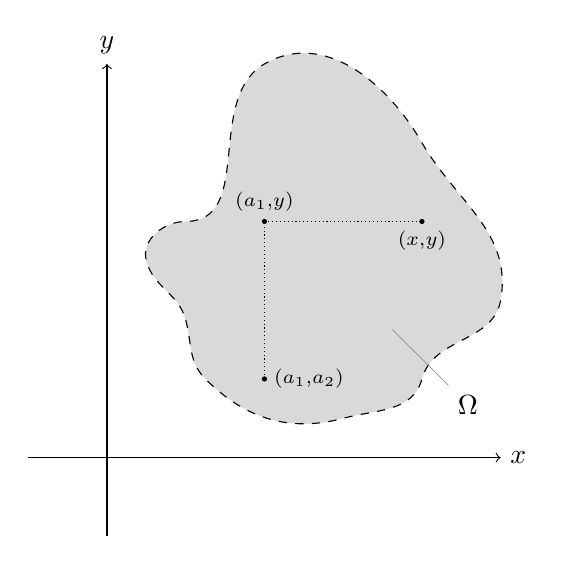
\begin{tikzpicture}
		\draw [black,->] (-1,0) -- (5,0) node[right]{$x$};
		\draw [black,->] (0,-1) -- (0,5) node[above]{$y$};
		\draw [fill=black!15!white,dashed] (1,1.75) to[out=-75,in=135] (1.25,1) to[out=-45,in=195] (3,.5) to[out=15,in=-105] (4,1) to[out=75,in=-100] (5,2) to[out=80,in=-60] (4,4) to[out=120,in=30] (2,5) to[out=210,in=0] (1,3) to[out=180,in=105] (.5,2.5) to[out=-75,in=105] (1,1.75);
		\node [pin={[pin distance=1cm]-45:{$\Omega$}}] at (3.5,1.75) {};
		\draw [densely dotted] (2,1) node[right]{$\scriptstyle(a_1,a_2)$} to (2,3) node[above]{$\scriptstyle(a_1,y)$};
		\draw [densely dotted] (2,3) -- (4,3) node[below]{$\scriptstyle(x,y)$};
		\node [fill=black,circle,scale=.2] at (2,1) {};
		\node [fill=black,circle,scale=.2] at (2,3) {};
		\node [fill=black,circle,scale=.2] at (4,3) {};
	\end{tikzpicture}
	\caption{Incremento $\vec x-\vec a$ scomposto nelle due direzioni lungo gli assi cartesiani in $\R^2$.}
	\label{fig:differenziale_totale}
\end{figure}

	Applicando il teorema di Lagrange a $f(\cdot,y)$ e $f(a_1,\cdot)$, che sono entrambe derivabili per ipotesi, dato che corrispondono alle derivate parziali rispettivamente in $x$ e $y$, si ottiene che
	\begin{equation}
		f(x,y)-f(a_1,y)=(x-a_1)\drp{f}{x}(\xi,y)\qtext{e} f(a_1,y)-f(a_1,a_2)=(y-a_2)\drp{f}{y}(a_1,\eta)
	\end{equation}
	per qualche $(\xi,y)$ e $(a_1,\eta)$ in $\Omega$.
	Il numeratore della \eqref{eq:difftot} si riscrive quindi come
	\begin{align*}
		&(x-a_1)\drp{f}{x}(\xi,y)+(y-a_2)\drp{f}{y}(a_1,\eta)-\bigg[(x-a_1)\drp{f}{x}(a_1,a_2)+(y-a_2)\drp{f}{y}(a_1,a_2)\bigg]=\\
		=&(x-a_1)\bigg[\drp{f}{x}(\xi,y)-\drp{f}{x}(a_1,a_2)\bigg]+(y-a_2)\bigg[\drp{f}{y}(a_1,\eta)-\drp{f}{y}(a_1,a_2)\bigg],
	\end{align*}
	il cui modulo è minore della somma dei moduli dei termini, quindi
	\begin{align*}
		\leq&\abs{x-a_1}\abs[\bigg]{\drp{f}{x}(\xi,y)-\drp{f}{x}(a_1,a_2)}+\abs{y-a_2}\abs[\bigg]{\drp{f}{y}(a_1,\eta)-\drp{f}{y}(a_1,a_2)}\leq\\
		\leq&\norm{\vec x-\vec a}\abs[\bigg]{\drp{f}{x}(\xi,y)-\drp{f}{x}(a_1,a_2)}+\norm{\vec x-\vec a}\abs[\bigg]{\drp{f}{y}(a_1,\eta)-\drp{f}{y}(a_1,a_2)}=\\
		=&\norm{\vec x-\vec a}\left[\abs[\bigg]{\drp{f}{x}(\xi,y)-\drp{f}{x}(a_1,a_2)}+\abs[\bigg]{\drp{f}{y}(a_1,\eta)-\drp{f}{y}(a_1,a_2)}\right].
	\end{align*}
	Allora la \eqref{eq:difftot} è maggiorata dal termine tra parentesi quadre.
	Per $\vec x\to\vec a$ si ha $(\xi,y)\to\vec a$ e anche $(a_1,\eta)\to\vec a$, e poiché le derivate parziali per ipotesi sono continue risulta che la \eqref{eq:difftot} tende a 0, quindi la $f$ è differenziabile in $\vec a$.
\end{proof}
Se $f$ è una funzione vettoriale da $\R^n$ a $\R^m$, il teorema richiede che tutte le derivate parziali $\drp{f_i}{x_j}$ con $1\leq i\leq m$ e $1\leq j\leq n$ siano continue in $\vec a$.

\begin{definizione}
Sia $\Omega$ un aperto di $\R^n$ e $f\colon\Omega\to\R$: si dice che $f\in\cont[1]{\Omega}$ se in ogni punto di $\Omega$ esistono e sono continue tutte le derivate parziali di $f$.
\end{definizione}
\begin{corollario}
Se una funzione appartiene alla classe $\cont[1]{\Omega}$, allora è differenziabile in tutto $\Omega$.
\end{corollario}
La dimostrazione segue immediatamente dal teorema precedente.

\section{Differenziazione di funzioni composte}
\begin{teorema}
	Sia $\Omega$ un insieme aperto in $\R^n$, $\vec a\in\Omega$ e $\vec f\colon\Omega\to\R^m$ differenziabile in $\vec a$; sia quindi $\vec g\colon\vec f(\Omega)\to\R^p$ differenziabile in $\vec b=\vec f(\vec a)$.
	Allora la funzione composta $\vec h=\vec g\circ\vec f\colon\Omega\to\R^p$ è differenziabile in $\vec a$, e vale la relazione
	\begin{equation} \label{eq:composizione_differenziali}
		\dd\vec h(\vec a;\cdot)=\dd\vec g(\vec b;\cdot)\circ\dd\vec f(\vec a;\cdot)=\dd\vec g\big(\vec b;\dd\vec f(\vec a;\cdot)\big),
	\end{equation}
	vale a dire che la jacobiana di $\vec h$ in $\vec a$ è il prodotto ordinato della jacobiana di $\vec g$ per quella di $\vec f$:
	\begin{equation}
		\jac\vec h(\vec a)=\jac\vec g\big(\vec f(\vec a)\big)\jac\vec f(\vec a).
	\end{equation}
	Il prodotto tra queste matrici è possibile, dato che sono rispettivamente $p\times m$ e $m\times n$, e si ottiene quindi che la jacobiana di $\vec h$ ha $p$ righe e $n$ colonne. Il prodotto \emph{non} è commutativo, in quanto non è nemmeno possibile eseguirlo scambiando l'ordine dei fattori, diversamente dal caso di funzioni da $\R$ in $\R$.
\end{teorema}
Sviluppando il prodotto tra le due matrici si ha che la componente della jacobiana di $\vec h$ è, con $1\leq i\leq p$ e $1\leq j\leq n$,
\[
\big(\!\jac\vec h(\vec a)\big)_{ij}=\drp{h_i}{x_j}(\vec a)=\sum_{k=1}^m\drp{g_i}{y_k}\big(\vec f(\vec a)\big)\drp{f_k}{x_j}(\vec a),
\]
dove $y_k$ è la variabile relativa a $\vec g$, ossia $y_k=f_k(\vec a)$.
\begin{teorema}[Lagrange] \label{t:lagrange_piu_variabili}
Sia $\Omega$ un aperto di $\R^n$, $\vec a$ e $\vec b$ due punti interni ad esso tali che $[\vec a,\vec b]\subset\Omega$, e $g\colon\Omega\to\R$ una funzione differenziabile in tutto $\Omega$. Allora esiste un punto $\vxi\in[\vec a,\vec b]$ per il quale $g(\vec b)-g(\vec a)=\inner{\grad g(\vxi)}{\vec b-\vec a}$.
\end{teorema}
\begin{proof}
Sul segmento $\vec b-\vec a$ si costruisce una funzione vettoriale $\vec f(t)=\vec a+t(\vec b-\vec a)$, con $t\in[0,1]$\footnote{Dato che tale segmento è chiuso e interno ad $\Omega$, anche ``sporgendo'' un poco oltre gli estremi si resterà sempre nell'insieme, quindi volendo si può limitare $t$ anche a $(-\epsilon,1+\epsilon)$}: componendola con $g$ si ottiene che $(g\circ\vec f)(t)=g[\vec a+t(\vec b-\vec a)]$, tale che $g\circ\vec f\colon[0,1]\to\R$ e le si applica il teorema \ref{t:lagrange} di Lagrange per funzioni reali a variabili reali nell'intervallo $[0,1]$, ottenendo che esiste $\theta\in(0,1)$ tale per cui $(g\circ\vec f)(1)-(g\circ\vec f)(0)=(g\circ\vec f)'(\theta)$, cioè
\[
g(\vec b)-g(\vec a)=\jac g\big(\vec f(\theta)\big)\jac\vec f=\inner{\grad g\big(\vec f(\theta)\big)}{\vec b-\vec a}.
\]
Il punto $\vec f(\theta)$ è il punto $\vxi$ cercato della tesi.
\end{proof}
Si potrebbe formulare una versione di questo teorema anche per le funzioni vettoriali, per il quale al posto del gradiente in $\vec a$ si avrebbe la jacobiana in $\vec a$: si applicherebbe semplicemente il teorema di Lagrange appena dimostrato per ognuna delle componenti di $\vec g$. In realtà un tale teorema non ha ragione di esistere, come mostra il seguente controesempio. Sia $\vec g(t)=(\cos t,\sin t)$, con $\vec a=0$ e $\vec b=2\pi$. Una versione vettoriale del teorema di Lagrange porterebbe a concludere che esisterebbe $x\in(0,2\pi)$ per cui
\[
\vec g(2\pi)-\vec g(0)=\begin{pmatrix}\grad g_1\\\grad g_2\end{pmatrix} 2\pi=\begin{pmatrix}-\sin x\\\cos x\end{pmatrix} 2\pi= \begin{pmatrix}1\\0\end{pmatrix}-\begin{pmatrix}1\\0\end{pmatrix}= \begin{pmatrix}0\\0\end{pmatrix},
\]
ossia $\sin x=0$ e $\cos x=0$ contemporaneamente, chiaramente assurdo.

Il problema sta nel fatto che sebbene sia realmente possibile applicare il teorema \ref{t:lagrange_piu_variabili} alle varie componenti di una funzione vettoriale, non si può affermare che sia soddisfatto per ognuna in un unico punto: ogni componente soddisfa il teorema in punti diversi.
\begin{teorema}[dell'incremento finito]
Sia $\Omega\in\R^m$ un aperto e $\vec g\colon\Omega\to\R^p$ differenziabile in $[\vec a,\vec b]\subset\Omega$. Allora esiste $c\geq 0$ tale per cui $\norm{\vec g(\vec b)-\vec g(\vec a)}\leq c\norm{\vec b-\vec a}$.
\end{teorema}
Un ``buon'' valore di questa quantità $c$ è ad esempio
\begin{equation*}
	c=\sqrt{mp}\max_{\substack{1\leq i\leq p\\1\leq j\leq m}}\sup_{\vec x\in[\vec a,\vec b]}\abs[\bigg]{\drp{g_i}{x_j}(\vec x)}.
\end{equation*}
ossia il valore maggiore tra tutte le derivate parziali, nell'intervallo dato, tra tutte le componenti di $\vec g$.
Se tutte le derivate parziali sono nulle, si ha $c=0$ quindi la funzione è costante.

\section{Diffeomorfismi}
\begin{definizione} \label{d:diffeomorfismo}
Siano $A\in\R^n$ e $B\in\R^n$ due insiemi aperti. Una funzione $\vec f\colon A\to B$ biiettiva si dice \emph{diffeomorfismo} di $A$ su $B$ se $\vec f$ è differenziabile e la sua inversa $\vec f^{-1}\colon B\to A$ è anch'essa differenziabile.
\end{definizione}
Anche l'inverso di un diffeomorfismo è ovviamente, a sua volta, un diffeomorfismo: in questa classe di funzioni si trovano in particolare i cambiamenti di coordinate, che infatti per queste proprietà si possono applicare senza problemi di irregolarità nelle funzioni.
\begin{teorema}
Sia $\vec f\colon A\to B$ con $A\in\R^n$ e $B\in\R^m$. Se risulta che:
\begin{itemize}
	\item $\vec f$ è differenziabile $\forall\vec x\in A$;
	\item ?
	\item $\det\jac\vec f(\vec x)$ per ogni $\vec x\in A$,
\end{itemize}
allora $\vec f$ è un diffeomorfismo.
\end{teorema}
Le traslazioni sono dei diffeomorfismi: sia ad esempio in $\R^3$ la funzione $\vec T(\vec x)=\vec x+\vec b$, essa è indubbiamente differenziabile, e lo è anche la sua inversa $\vec T^{-1}(\vec x)=\vec x-\vec b$.
Calcolando le matrici jacobiane di queste funzioni si ha
\[
\jac\vec T(\vec x)=\jac\vec T^{-1}(\vec x)=\begin{bmatrix}
1&0&0\\0&1&0\\0&0&1
\end{bmatrix}
\]
per ogni $\vec x\in\R^3$, generalizzabile ovviamente a qualunque dimensione.
Si nota che il prodotto delle due jacobiane dà la matrice identità $3\times 3$: questo non è dovuto al fatto che entrambe le jacobiane sono già di per sé matrici identità, ma è un risultato generale per tutti i diffeomorfismi. Se infatti si compongono una funzione $\vec f$ con la sua inversa $\vec f^{-1}$, si ottiene l'identità $\vec f^{-1}\circ\vec f=\textup{id}_A$ sull'insieme $A$; calcolando le jacobiane,
\[
\jac(\vec f^{-1}\circ\vec f)(\vec x)=\jac\vec f^{-1}\big(\vec f(\vec x)\big)\jac \vec f(\vec x)=\jac\vec x=I_n,
\]
che è la jacobiana della funzione identità, per ogni $\vec x\in A$. Di conseguenza, passando ai determinanti si trova che $\det\jac \vec f(\vec x)\neq 0$, e che essa è l'inversa di $\jac\vec f^{-1}\big(\vec f(\vec x)\big)$.

\begin{esempio} \label{es:diffeomorfismo-coordinate-polari-R2}
	Tra i diffeomorfismi più importanti si trovano i cambiamenti di coordinate, come quello in coordinate polari: esso è una trasformazione biunivoca tra $\R^2$ privato dell'origine e $(0,+\infty)\times[0,2\pi)$, che porta la coppia di coordinate cartesiane $(x,y)$ nella coppia $(\rho,\theta)$, che indica rispettivamente la distanza dall'origine degli assi e l'angolo che la retta congiungente l'origine e il punto formerebbe con il semiasse positivo delle ascisse, con le trasformazioni
	\begin{equation}
	\begin{cases}
	\rho=\sqrt{x^2+y^2}\\
	x=\rho\cos\theta\\
	y=\rho\sin\theta
	\end{cases}.
	\end{equation}
	Sia $\vec T\colon(0,+\infty)\times[0,2\pi)\to\R^2\setminus\{(0,0)\}$ definita come $\vec T\colon(\rho,\theta)\mapsto(\rho\cos\theta,\rho\sin\theta)=(x,y)$: il determinante della jacobiana della trasformazione è sempre non nullo, infatti
	\[
	\det\jac\vec T(\rho,\theta)=
		\begin{vmatrix}
		\cos\theta	&-\rho\sin\theta\\
		\sin\theta	&\rho\cos\theta
		\end{vmatrix}
	=\rho(\cos^2\theta+\sin^2\theta)=\rho\neq 0
	\]
	essendo definito in $(0,+\infty)$, quindi è un diffeomorfismo.
	Posta $f$ una funzione qualunque da $\R^2\setminus\{(0,0)\}$ a $\R$ (per semplicità), si può comporre con $\vec T$ ottenendo
	\[
	g(\rho,\theta)=f\big(\vec T(\rho,\theta)\big).
	\]
	Si ricava $f(x,y)$ invertendo il processo:
	\[
	f(x,y)=g\big(\vec T^{-1}(x,y)\big).
	\]
	Calcolando le jacobiane, risulta allora per la $g$
	\begin{equation} \label{eq:composizione_jacobiane_polari1}
	\jac g(\rho,\theta)=\jac f\big(\vec T(\rho,\theta)\big)\jac\vec T(\rho,\theta)
	\end{equation}
	mentre per la $f$ si ha
	\begin{multline} \label{eq:composizione_jacobiane_polari2}
	\jac f(x,y)=\jac g\big(\vec T^{-1}(x,y)\big)\jac\vec T^{-1}(x,y)=\\
	=\jac g\big(\vec T^{-1}(x,y)\big)\big[\jac\vec T\big(\vec T^{-1}(x,y)\big)\big]^{-1}=\jac g\big(\vec T^{-1}(x,y)\big)\big[\jac\vec T(\rho,\theta)\big]^{-1},
	\end{multline}
	sfruttando il fatto che $\jac\vec T\big(\vec T^{-1}(x,y)\big)=\jac\vec T(\rho,\theta)$ è l'inversa di $\jac\vec T^{-1}(x,y)$, come visto in precedenza.

	Dalle \eqref{eq:composizione_jacobiane_polari1} e \eqref{eq:composizione_jacobiane_polari2} si possono dunque calcolare le formule per la derivazione in coordinate polari: esse sono
	\begin{equation} \label{eq:jacobiane_polari}
	\begin{gathered}
	\grad g(\rho,\theta)
	=\grad f(x,y)
		\begin{pmatrix}
		\cos\theta	&-\rho\sin\theta\\
		\sin\theta	&\rho\cos\theta
		\end{pmatrix}\\
	\grad f(x,y)
	=\grad g(\rho,\theta)
		\begin{pmatrix}
		\cos\theta			&\sin\theta\\
		-\frac{\sin\theta}{\rho}	&\frac{\cos\theta}{\rho}
		\end{pmatrix}
	=\bigg(\drp{g}{\rho},\drp{g}{\theta}\bigg)
		\begin{pmatrix}
		\frac{x}{\sqrt{x^2+y^2}}	&\frac{y}{\sqrt{x^2+y^2}}\\
		-\frac{y}{x^2+y^2}		&\frac{x}{x^2+y^2}.
		\end{pmatrix},
	\end{gathered}
	\end{equation}
	dunque le derivate della funzione dopo la trasformazione in coordinate polari sono
	\begin{equation} \label{eq:derivate_polari}
	\begin{gathered}
	\drp{g}{\rho}=\cos\theta\,\drp{f}{x}+\sin\theta\,\drp{f}{y}\\
	\drp{g}{\theta}=-\rho\sin\theta\,\drp{f}{x}+\rho\cos\theta\,\drp{f}{y}.
	\end{gathered}
	\end{equation}
\end{esempio}

\section{Derivate seconde}
Sia $f$ una funzione scalare definita da un aperto $\Omega\subset\R^n$ a $\R$, e si supponga che per ogni $\vec x\in\Omega$ esista la derivata $D_{\vec v}f(\vec x)$, lungo la direzione indicata dal versore $\vec v$. Fissato un altro versore $\vec w$, se esiste la derivata di questa derivata lungo $\vec w$ in un punto $\vec a$, ossia $D_{\vec w}\big(D_{\vec v}f(\vec a)\big)$, che equivale al limite
\[
\lim_{t\to 0}\frac{D_{\vec v}f(\vec a+t\vec w)-D_{\vec v}f(\vec a)}{t},
\]
allora si dice che $f$ è due volte derivabile in $\vec a$ lungo le direzioni $\vec v$ e $\vec w$, \emph{rigorosamente nell'ordine} rappresentato. Tale derivata seconda si scrive come $D^2_{\vec v,\vec w}f(\vec a)$, indicando nei pedici i due versori, nell'ordine della prima e della seconda derivata.
Se inoltre i versori appartengono alla base canonica di $\R^n$, allora la derivata si scrive anche come
\[
D^2_{\vec e_i,\vec e_j}f(\vec a)=\frac{\partial^2f}{\partial x_i\partial x_j}(\vec a).
\]
Le derivate parziali seconde con versori differenti si dicono miste.

Se esistono tutte le derivate seconde parziali in $\vec a$ di $f$ (in tutto sono $n^2$) allora esse formano, in ordine, una matrice quadrata $n\times n$, detta \emph{matrice hessiana} di $f$ in $\vec a$ (da valutare nel punto):
\[
\hes f=\begin{bmatrix}
\dfrac{\partial^2f}{\partial x_1^2}		&\dfrac{\partial^2f}{\partial x_1\partial x_2}	&\cdots 	&\dfrac{\partial^2f}{\partial x_1\partial x_n}\\
\dfrac{\partial^2f}{\partial x_2\partial x_1}	&\dfrac{\partial^2f}{\partial x_2^2}		&\cdots 	&\dfrac{\partial^2f}{\partial x_2\partial x_n}\\
\vdots 							&\vdots 							&\ddots 	&\vdots\\
\dfrac{\partial^2f}{\partial x_n\partial x_1}	&\dfrac{\partial^2f}{\partial x_n\partial x_2}	&\cdots 	&\dfrac{\partial^2f}{\partial x_n^2}
\end{bmatrix}\qquad\qquad(\hes f)_{ij}=\dfrac{\partial^2f}{\partial x_i\partial x_j}.
\]
L'hessiana di fatto rappresenta la jacobiana del gradiente come vettore riga.

L'ordine di derivazione è importante non solo per il risultato dell'operazione, ma anche per l'esistenza stessa del risultato, come dimostrano i seguenti esempi in $\R^2$.
\begin{esempio} \label{es:ordine-di-derivazione-1}
	Sia $f(x,y)=x^2y^{1/3}$. Le derivate prime parziali nell'origine sono entrambe nulle, altrimenti
	\[
	\drp{f}{x}(x,y)=2x\sqrt[3]{y}\qtext{e}\drp{f}{y}(x,y)=\begin{dcases*}\nexists&in $(x,0)$ con $x\neq 0$\\\frac{x^2}{3y^{2/3}}&altrove\end{dcases*}.
	\]
	Nell'origine, la derivata seconda rispetto a $y$ e poi a $x$, nell'ordine, ossia $\drp{}{x}\big(\drp{f}{y}\big)(0,0)$, non esiste, mentre la derivata seconda rispetto a $x,y$ è
	\[
	\frac{\partial^2f}{\partial x\partial y}(x,y)=\drp{}{y}\bigg(\drp{f}{x}\bigg)(0,0)=\lim_{y\to 0}\frac{\drp{f}{x}(0,y)-\drp{f}{x}(0,0)}{y}=0.
	\]
\end{esempio}
\begin{esempio} \label{es:ordine-di-derivazione-2}
	Sia $f$ definita come
	\[
	f(x,y)=\begin{dcases*}0&in $(0,0)$\\\frac{xy^3}{x^2+y^2}&altrove\end{dcases*}.
	\]
	Nell'origine si ha $\grad f(0,0)=(0,0)$, altrimenti il gradiente di $f$ è
	\[
	\grad f(x,y)=\bigg(\frac{y^5-x^2y^3}{(x^2+y^2)^2},\frac{3x^3y^2+xy^4}{(x^2+y^2)^2}\bigg).
	\]
	Allora si ha
	\begin{align*}
	&\frac{\partial^2f}{\partial y\partial x}=\lim_{x\to 0}\frac{\drp{f}{y}(x,0)-\drp{f}{y}(0,0)}{x}=\lim_{x\to 0}\frac0{x}=0,\\
	%in che punti???
	&\frac{\partial^2f}{\partial x\partial y}=\lim_{y\to 0}\frac{\drp{f}{x}(0,y)-\drp{f}{x}(0,0)}{y}=\lim_{y\to 0}\frac{y}{y}=1.
	\end{align*}
\end{esempio}
Per certe funzioni, però, le derivate seconde non dipendono dall'ordine di derivazione, come spiegato dal seguente teorema.
\begin{teorema}[Schwarz] \label{t:schwarz}
Siano $\Omega$ un aperto di $\R^n$, $\vec a$ un punto interno ad esso, $\vec v$ e $\vec w$ due versori di $\R^n$ e $f$ una funzione definita da $\Omega$ a $\R$. Se esiste un intorno di $\vec a$ contenuto in $\Omega$ in cui esistono sia $D^2_{\vec v,\vec w}f$ che $D^2_{\vec w,\vec v}f$ e sono continue in $\vec a$, allora esse coincidono in tale punto.
\end{teorema}
\begin{corollario}
Se la funzione $f$ è di classe $\cont[2]{\Omega}$, cioè esistono e sono continue tutte le derivate parziali prime e seconde in $\Omega$, allora le derivate miste coincidono; vale a dire, la matrice hessiana è simmetrica.
\end{corollario}
Se la funzione poi è vettoriale, la matrice hessiana avrà dei vettori come componenti, e il teorema di Schwarz vale ancora componente per componente.%?

Quando $f\colon\Omega\to\R$ è differenziabile in ogni punto $\vec x\in\Omega$, il suo differenziale primo $\dd f(\vec x;\cdot)$ è una funzione da $\R^n$ a $\R$ lineare, definita come $\dd f(\vec x;\vec h)=\inner{\grad f(\vec x)}{\vec h}$, $\forall\vec h$ tale che l'incremento $\vec x+\vec h$ appartenga ancora ad $\Omega$. Fissato però l'incremento $\vec h$, si può considerare $\dd f(\cdot;\vec h)=\inner{\grad f(\cdot)}{\vec h}$ che è una funzione di variabile $\vec x\in\Omega$ a valori reali, proprio come $f$. Se questa funzione\footnote{Poiché le derivate parziali sono $n$ e non una sola, in realtà il differenziale primo come $\dd f(\cdot;\vec h)$ rappresenta più di una funzione: è la combinazione lineare delle derivate parziali.} $\dd f(\cdot;\vec h)$ è differenziabile in un punto $\vec a$ di $\Omega$, allora si dice che $f$ è due volte differenziabile in $\vec a$.

Alcune condizioni implicano o sono implicate dal fatto che $f$ è due volte differenziabile in $\vec a$:
\begin{enumerate}
\item (\textit{necessaria e sufficiente}) ogni derivata parziale prima è differenziabile in $\vec a$;
\item (\textit{necessaria}) esistono tutte le derivate parziali seconde in $\vec a$, e quelle miste coincidono\footnote{Questa affermazione non equivale al teorema \ref{t:schwarz} di Schwarz, in quanto le ipotesi sono differenti.};
\item (\textit{necessaria}) ogni derivata direzionale prima è differenziabile in $\vec a$, quindi esistono tutte le derivate seconde direzionali indipendentemente dell'ordine (per il punto precedente) e si ha
\[
D^2_{\vec v,\vec w}f(\vec a)=\sum_{i,j=1}^n\frac{\partial^2f}{\partial x_i\partial x_j}(\vec a)v_iw_j,
\]
la quale è chiamata \emph{forma quadratica} di $f$ in $\vec a$;
\item (\textit{sufficiente}) in un intorno di $\vec a$ esistono e sono continue tutte le derivate prime parziali, ed esistono tutte le derivate seconde parziali e sono continue in $\vec a$;
\item (\textit{sufficiente}) $f$ è di classe $\cont[2]{\Omega}$.
\end{enumerate}

\section{Formula di Taylor}
Sia $f\colon\Omega\to\R$, con $\Omega\subseteq\R^n$ e $\vec a\in\Omega$. La $f$ si dice $k$-volte differenziabile in $\vec a$ se esiste il $(k-1)$-esimo differenziale della funzione nel punto.
La generica derivata parziale $k$-esima di $f$ si può allora scrivere come
\[
\frac{\partial^kf}{\partial x_1^{j_1}\dots\partial x_n^{j_n}},
\]
con $0\leq j_1,\dots,j_n\leq n$ e $\sum_{i=1}^nj_i=k$; gli indici $j_i$ indicano quante volte si sta derivando $f$ rispetto alla $i$-esima componente.
Per comodità si può eventualmente usare una notazione multiindice $\vec j=(j_i,\dots,j_n)$, con $\vec j\in\N^n$.

Sia quindi $f$ una funzione differenziabile $k$ volte in $\vec a$: si costruisce la mappa
\begin{equation} \label{eq:diff-kesimo}
\dd^kf(\vec a;\cdot;\dots;\cdot)\colon\underbracket[.5pt]{\R^n\times\dots\times\R^n}_\text{$k$ volte}\to\R,
\end{equation}
che è lineare in ogni variabile e tale per cui
\begin{equation}
\dd^kf(\vec a;\vec h^{(1)};\dots;\vec h^{(k)})=
\sum_{i_1,\dots,i_k}^n\frac{\partial^kf}{\partial x_{i_1}\dots\partial x_{i_n}}
h_{i_1}^{(1)}\dots h_{i_n}^{(k)}.
\end{equation}
Questa formula è utile nel caso in cui $\vec h^{(1)}=\dots=\vec h^{(k)}=\vec h\in\R^n$, per il quale si impiega un unico vettore per l'incremento per tutte le componenti: per snellire la notazione allora si scrive più semplicemente
\[
\dd^kf(\vec a;\underbracket[.5pt]{\vec h;\dots;\vec h}_\text{$k$ volte})=\dd^kf(\vec a;\vec h).
\]
Con questa notazione si può scrivere dunque
\begin{equation}
\dd^kf(\vec a;\vec h)=\sum\frac{\partial^kf}{\partial x_1^{j_1}\dots\partial x_n^{j_n}} h_1^{j_1}\dots h_n^{j_n},
\end{equation}
ancora con $0\leq j_1,\dots,\leq k$ e $\sum_{i=1}^n=k$, dove $k$ è l'ordine del differenziale. Il differenziale di ordina $k$ è quindi%? quindi cosa, che non si capisce un cazzo
 composto da una somma di monomi ciascuno di grado $k$, cioè è un polinomio omogeneo di grado $k$, nelle componenti del vettore $\vec h$.

Per come è composto il differenziale si ha quindi che sostituendo all'incremento fissato $\vec h$ un incremento variabile lungo la stessa direzione, ossia $t\vec h$, risulta
\begin{equation}
\dd^kf(\vec a;t\vec h)=t^k\dd^kf(\vec a;\vec h).
\end{equation}
Dividendo il differenziale per $\norm{\vec h}^k$ si ottiene dunque un polinomio omogeneo di grado nullo, e costante quando valutato sulle semirette con origine sull'origine degli assi\footnote{Non è corretto affermare che sia costante valutato sulle \emph{rette} passanti per l'origine, poiché per $\vec h=\vec 0$ la funzione non è definita, dato che il denominatore è nullo.}, infatti
\[
\frac{\dd^kf(\vec a;t\vec h)}{\norm{t\vec h}^k}=\frac{t^k\dd^kf(\vec a;\vec h)}{\abs{t}^k\norm{\vec h}^k}=\frac{\dd^kf(\vec a;\vec h)}{\norm{\vec h}^k}
\]
che è indipendente da $t$ quindi costante su tutta la semiretta.

Siano ora $\vec w\neq\vec 0$ e $f\in\cont[k]{\Omega}$. Per $t$ sufficientemente piccolo, $\vec a+t\vec w\in\Omega$, quindi la funzione $F(t)\defeq f(\vec a+t\vec w)$ è di classe $\cclass[k]$ in un intorno di $t=0$, dove è assicurato che sia composta da due funzioni una, $f$, di classe $\cclass[k]$ per definizione, e l'altra, $\vec a+t\vec w$, di classe $\cclass[\infty]$. Al di fuori di $\mathcal U(0)$ non è più certo che $\vec a+t\vec w$ appartenga ancora a $\Omega$, al di fuori del quale $f\notin\cclass[k]$. Dunque la $F$ è una funzione definita da $\mathcal U(0)$ a $\R$. Nel centro $t=0$ si può dunque sviluppare in serie di Taylor fino all'ordine $k$: le sue derivate sono
\begin{equation}\begin{aligned}
F'(t)	&=\inner{\grad f(\vec a+t\vec w)}{\vec w}=\sum_{j=1}^n\drp{f}{x_j}(\vec a+t\vec w)w_j=\dd f(\vec a+t\vec w;\vec w)\\
F''(t)	&=\sum_{j=1}^nw_j\bigg[\sum_{i=1}^n\drp{}{x_i}\Big(\drp{f}{x_j}(\vec a+t\vec w)w_i\Big)\bigg]=\\
		&=\sum_{i,j=1}^n\frac{\partial^2f}{\partial x_i\partial x_j}(\vec a+t\vec w)w_iw_j=\\
		&=\vec w^T\hes f(\vec a+t\vec w)\vec w=\dd^2f(\vec a+t\vec w;\vec w),
\end{aligned}\end{equation}
e così via per induzione %ma dove???
si ha $F^{(n)}(t)=\dd^nf(\vec a+t\vec w;\vec w)$, per ogni $0\leq n\leq k$.
Operando il cambio di variabile $\vec x\defeq\vec a+\vec w$ (con il segmento $[\vec a,\vec x]\subset\Omega$) lo sviluppo di Taylor di $F$ con resto di Lagrange, centrato in $t=0$, nell'intervallo $[0,1]$ è
\[
F(1)=\frac1{0!}F(0)1^0+\frac1{1!}F'(0)1^1+\frac1{2!}F''(0)1^2+\dots+\frac1{(k-1)!}F^{(k-1)}(0)1^{k-1}+\frac1{k!}F^{(k)}(\theta)
\]
per qualche $\theta\in(0,1)$. Per la definizione di $F$ quindi risulta, dato che $F(1)=f(\vec x)$, che
\begin{multline} \label{eq:formula_taylor_lagrange_piu_variabili}
f(\vec x)=f(\vec a)+\dd f(\vec a;\vec x-\vec a)+\frac1{2!}\dd^2f(\vec a;\vec x-\vec a)+\dots\\
\dots+\frac1{(k-1)!}\dd^{k-1}f(\vec a;\vec x-\vec a)+\frac1{k!}\dd^kf(\vxi;\vec x-\vec a)
\end{multline}
dove $\vxi\in(\vec a,\vec x)$, corrispondente al punto $\theta$ precedente.

Con il resto di Peano, invece, si ha, sempre all'ordine $k$,
\begin{equation} \label{eq:formula_taylor_peano_piu_variabili}
f(\vec x)=\sum_{j=0}^k\frac1{j!}\dd^jf(\vec a;\vec x-\vec a)+o(\norm{\vec x-\vec a}^k).
\end{equation}

\section{Estremanti liberi}
\begin{definizione}
Sia $f\colon\Omega\to\R$ dove $\Omega\in\R^n$ e sia $\vec a\in\Omega$. Il punto $\vec a$ si dice punto di estremo locale per $f$ in $\Omega$, e in particolare:
\begin{itemize}
\item \emph{punto di massimo locale} se $\exists B(\vec a,r)\subset\Omega$ in cui $f(\vec a)\geq f(\vec x)$, per ogni $\vec x\in B(\vec a,r)$;
\item \emph{punto di minimo locale} se $\exists B(\vec a,r)\subset\Omega$ in cui $f(\vec a)\leq f(\vec x)$, per ogni $\vec x\in B(\vec a,r)$.
\end{itemize}
\end{definizione}
Il massimo o il minimo locale sono il valore assunto dalla funzione nel rispettivo punto estremante. Il massimo è assoluto se la definizione è estendibile a tutto l'insieme $\Omega$, cioè se $f(\vec a)\geq f(\vec x)$ per ogni $\vec x\in\Omega$; analogamente per i minimi.
Infine, il punto estremante si dice \emph{forte} se l'uguaglianza si ha solo in $\vec a$ e non anche altrove.

Si ricorda il teorema di Weierstrass \ref{t:weierstrass} che afferma che se $f$ è continua in $E$ compatto, allora essa ha massimo e minimo assoluti in $E$. Individuato questo insieme compatto, gli estremi (locali) possono trovarsi in $\interior{E}$ o in $\boundary E$: in questi casi si dicono, rispettivamente, estremi \emph{liberi} ed estremi \emph{vincolati}. Se individuare gli estremi vincolati in una sola dimensione consisteva al più nell'analisi di due soli punti, in più dimensioni la frontiera di un insieme è solitamente costituita da infiniti punti: occorrono quindi metodi diversi per i due casi.
Di seguito ci si occuperà soltanto degli estremi liberi.

\begin{teorema}[Fermat]
Sia $f\colon\Omega\to\R$, con $\Omega\in\R^n$ aperto, differenziabile in $\vec a\in\Omega$. Se $\vec a$ è un punto estremante per $f$, allora $\grad f(\vec a)=\vec 0$.
\end{teorema}
\begin{proof}
Si consideri l'incremento della $f$ lungo la direzione data dal versore $\vec e_i$ della base canonica
\[
g_i(t)=f(\vec a+t\vec e_i).
\]
Sia ora $\vec a$ un punto di massimo: allora $f(\vec a)\geq f(\vec a+t\vec e_i)$ per ogni $t$ opportunamente contenuto in un intervallo $(-\delta,\delta)$ tale che $f$ sia ancora differenziabile in $\vec a\pm\delta\vec e_i$, quindi per cui $g_i$ è derivabile in $(-\delta,\delta)$.
Dunque si ha $g_i(t)-g_i(0)\leq 0$, sia per $-\delta<t<0$ che per $0<t<\delta$; dividendo entrambi gli incrementi per $t$ e passando al limite rispettivamente per $t\to0^\mp$, si ottiene la derivata sinistra e destra di $g_i$ in $0$, che per il teorema di permanenza del segno sono rispettivamente non negativa e non positiva. Poiché $g$ è derivabile in $0$, le derivate devono coincidere e non può che risultare
\[
\lim_{t\to 0^-}g'_i(t)=\lim_{t\to 0^+}g'_i(t)=g_i'(0)=\drp{f}{x_i}(\vec a)=0,
\]
questo naturalmente per ogni $i\in\{1,\dots,n\}$, cioè tutte le derivate parziali di $f$ sono nulle in $\vec a$: allora $\grad f(\vec a)=\vec 0$.
\end{proof}
Ovviamente la condizione data è soltanto sufficiente, come mostra la funzione $f(x)=x^2-y^2$, che nell'origine ha gradiente nullo ma tale punto non è un estremante; i punti stazionari non estremanti si dicono \emph{punti di sella}. In ogni caso, è necessaria soltanto per i punti estremanti \emph{liberi}, dato che $\Omega$ è aperto, e in cui $f$ è differenziabile. Rimangono esclusi quindi i punti in cui $f$ non è differenziabile, da analizzare singolarmente, e gli estremi vincolati.

Sia $f\in\cont[2]{\Omega}$. In $\vec a$, punto estremante locale di $f$, il gradiente è nullo: per $\vec h\to\vec 0$, arbitrariamente piccolo e tale per cui $\vec a+\vec h\in\Omega$, per il teorema di Taylor con resto di Peano risulta
\begin{align}
&f(\vec a+\vec h)=f(\vec a)+\inner{\grad f(\vec a)}{\vec h}+\frac12\dd^2f(\vec a;\vec h)+o(\norm{\vec h}^2)\\
&f(\vec a+\vec h)-f(\vec a)=\frac12\dd^2f(\vec a;\vec h)+o(\norm{\vec h}^2).
\end{align}
Sfruttando l'uguaglianza %da dimostrare!
$\dd^2f(\vec a;\vec h)=\vec h^T\hes f(\vec a)\vec h$, e in seguito raccogliendo $\norm{\vec h}^2$ si ottiene l'equazione
\begin{equation}
f(\vec a+\vec h)-f(\vec a)=\frac12\norm{\vec h}^2\left[\frac{\vec h^T\hes f(\vec a)\vec h}{\norm{\vec h}^2}+o(1)\right].
\end{equation}
Il segno del secondo membro, che sarà quindi il segno dell'incremento della funzione da $\vec a$ a $\vec a+\vec h$, è quindi determinato dalla forma quadratica $\vec h^T\hes f(\vec a)\vec h$. Si $F(\vec h)$ la funzione definita come
\[
F(\vec h)=\frac{\vec h^T\hes f(\vec a)\vec h}{\norm{\vec h}^2}.
\]
Essa è una funzione omogenea di grado 0, quindi è costante sulle semirette con origine nell'origine degli assi\footnote{Le forme quadratiche sono polinomi omogenei di grado 2, quindi dividendole per una norma al quadrato, anch'essa di grado 2, si ottiene un polinomio di grado nullo.}: infatti fissato $\vec v$ e per $t>0$ si ha
\[
F(t\vec v)=\frac{(t\vec v)^T\hes f(\vec a)(t\vec v)}{\norm{t\vec v}^2}=\frac{t^2}{\abs{t}^2}\frac{\vec v^T\hes f(\vec a)\vec v}{\norm{\vec v}^2}=F(\vec v).
\]
La $F$ è dunque definita in $\R^n\setminus\{\vec 0\}$, è continua e differenziabile dove definita, e costante quando ristretta alle rette passanti per l'origine. Si possono allora analizzare i valori assunti da $F$ su una superficie sferica qualsiasi centrata nell'origine, ad esempio fissando $\norm{\vec h}=1$. Questa superficie, che corrisponde poi a $\boundary B(\vec 0,1)$, è chiusa e limitata, cioè è un insieme compatto. Per il teorema di Weierstrass dunque la $F$ ammette un minimo e un massimo assoluto $m,M$ in $\boundary B(\vec 0,1)$, cioè esistono $\vec u,\vec w\neq\vec 0$ tali per cui
\begin{equation} \label{eq:maxmin_quadratica}
m=F(\vec u)\leq F(\vec h)\leq F(\vec w)=M.
\end{equation}
Per il teorema di Fermat, allora, si ha $\grad f(\vec u)=\grad f(\vec w)=\vec 0$.
Nel caso in cui $mM\neq 0$ risulta:
\begin{itemize}
\item se $0<m\leq M$, $F$ assume soltanto valori tra $m$ e $M$ che sono entrambi positivi, quindi $F(\vec h)>0$ e per $\norm{\vec h}$ sufficientemente piccolo il termine $o(\norm{\vec h}^2)$ non influisce sul segno, quindi si ha $f(\vec a+\vec h)-f(\vec a)>0$ cioè $\vec a$ è un punto di minimo locale;
\item analogamente se $m\leq M<0$, $\vec a$ è un punto di massimo locale;
\item se $m<0<M$, la $F$ cambia di segno, quindi $\vec a$ è un punto di sella.
\end{itemize}
Quando invece $mM=0$, il segno è determinato da $o(\norm{\vec h}^2)$, quindi questo metodo non porta ad alcun risultato.
Rimane quindi da trovare il segno di $m$ e $M$. Poiché $f$ è differenziabile due volte, la sua matrice hessiana è simmetrica, e come già visto si può rappresentare (fissata la base, cioè quella canonica) la forma quadratica che è il differenziale secondo con l'espressione $\vec h^T\hes f(\vec a)\vec h$. Sia quindi $q(\vec x)=\vec x^T\hes f(\vec a)\vec x$: si ha che $F(\vec x)=q(\vec x)/\norm{\vec x}^2$, e vale ancora la \eqref{eq:maxmin_quadratica}.
Le derivate parziali di $F$ sono
\[
\drp{}{x_k}\norm{\vec x}^2=\drp{}{x_k}\bigg(\sum_{i=1}^nx_i^2\bigg)=2x_k,
\]
e
\[\begin{split}
\drp{}{x_k}q(\vec x)	&=\drp{}{x_k}\bigg(\sum_{i,j=1}^n\big(\hes f(\vec a)\big)_{ij}x_ix_j\bigg)=\\
					&=\sum_{i,j=1}^n\big(\hes f(\vec a)\big)_{ij}(\delta_{ik}x_j+\delta_{jk}x_i)=\\
					&=\sum_{j=1}^n\big(\hes f(\vec a)\big)_{kj}x_j+\sum_{i=1}^n\big(\hes f(\vec a)\big)_{ik}x_i=\\
					&=\sum_{j=1}^n\big(\hes f(\vec a)\big)_{kj}x_j+\sum_{i=1}^n\big(\hes f(\vec a)\big)_{ki}x_i=\\
					&=2\sum_{j=1}^n\big(\hes f(\vec a)\big)_{kj}x_j=\\
					&=2\big(\hes f(\vec a)\vec x\big)_j
\end{split}\]
dove si è potuto cambiare gli indici dell'hessiana da $ik$ a $ki$ poiché è simmetrica.
Allora risulta
\[\begin{split}
\drp{}{x_k}F(\vec x)	&=\norm{\vec x}^{-4}\left[\norm{\vec x}^2\drp{q}{x_k}(\vec x)-q(\vec x)\drp{}{x_k}\norm{\vec x}^2\right]=\\
					&=\norm{\vec x}^{-4}\left[\norm{\vec x}^22\big(\hes f(\vec a)\vec x\big)_k-q(\vec x)2x_k\right],
\end{split}\]
dunque
\begin{equation}
\begin{split}
\grad F(\vec x)	&=2\norm{\vec x}^{-4}\big[\norm{\vec x}^2\hes f(\vec a)\vec x-q(\vec x)\vec x\big]=\\
				&=\frac2{\norm{\vec x}^2}\left[\hes f(\vec a)\vec x-\frac{q(\vec x)\vec x}{\norm{\vec x}^2}\right].
\end{split}
\end{equation}
Nei punti $\vec u$ e $\vec v$ estremanti di $F$ si ha dunque $\grad F(\vec x)=\vec 0$, quindi dato che $\vec x$ non è nullo si ha
\begin{equation}
\hes f(\vec a)\vec x=\frac{q(\vec x)}{\norm{\vec x}^2}\vec x=F(\vec x)\vec x,
\end{equation}
cioè $F(\vec x)$ è un autovalore di $\hes f(\vec a)$ a cui è associato proprio l'autovettore $\vec x$. Gli autovalori della matrice hessiana sono tanti quanti la dimensione di $\R^n$, e poiché è simmetrica, sono tutti reali.
Di conseguenza il massimo autovalore di $\hes f(\vec a)$ è anche il massimo di $F(\vec x)$, e lo stesso per il minimo: individuando gli autovalori dell'hessiana in $\vec a$ si trova quindi la natura del punto estremante.
La forma quadratica $q(\vec x)=\vec x^T\hes f(\vec a)\vec x$ si dice
\begin{itemize}
\item\emph{definita positiva} se $q(\vec x)>0$, che significa $0<m\leq M$;
\item\emph{semidefinita positiva} se $q(\vec x)\geq 0$, cioè esiste $\vec v\neq\vec 0$ per cui $q(\vec v)=0$, e questo corrisponde a $0\leq m\leq M$;
\item\emph{indefinita} se esistono $\vec y,\vec z$ tali che $q(\vec y)<0<q(\vec z)$, cioè $m<0<M$;
\item\emph{semidefinita negativa} se $q(\vec x)\leq 0$, cioè $m\leq M\leq 0$;
\item\emph{definita negativa} se $q(\vec x)<0$, che significa $m\leq M<0$,
\end{itemize}
ovviamente per $\vec x\neq\vec 0$ in cui $q(\vec x)=0$ in ogni caso.
Si giunge quindi ai seguenti risultati:
\begin{itemize}
\item se $m>0$, $\vec a$ è un punto di minimo locale forte;
\item se $M<0$, $\vec a$ è un punto di massimo locale forte;
\item se $m<0<M$, $\vec a$ è un punto di sella;
\item se $\vec a$ è un punto di minimo locale (qualsiasi), $q(\vec x)$ è semidefinita positiva;
\item se $\vec a$ è un punto di massimo locale (qualsiasi), $q(\vec x)$ è semidefinita negativa.
\end{itemize}
Se $f$ è una funzione a due sole variabili, ha due autovalori per quanto detto in precedenza: il polinomio caratteristico dell'hessiana è
\begin{equation}\begin{split}
P(\lambda)=\det(\hes f(\vec a)-\lambda I_n)	&=\begin{vmatrix}f_{xx}(\vec a)-\lambda&f_{xy}(\vec a)\\f_{xy}(\vec a)&f_{yy}(\vec a)-\lambda\end{vmatrix}=\\
										&=\lambda^2-(f_{xx}+f_{yy})\lambda+(f_{xx}f_{yy}-f_{xy}^2)=\\
										&=\lambda^2-\big(\tr\hes f(\vec a)\big)\lambda+\det\hes f(\vec a).
\end{split}\end{equation}
Poiché è utile ai fini di conoscere la natura del punto estremante solo sapere il segno degli autovalori, cioè delle due radici del polinomio, e dato che $P(\lambda)=(\lambda-m)(\lambda-M)$, si ha che $m+M=\tr\hes f(\vec a)$ e $mM=\det\hes f(\vec a)$, quindi:
\begin{itemize}
\item se $\det\hes f(\vec a)=0$, non si può affermare niente;
\item se $\det\hes f(\vec a)>0$, si considera la somma delle radici, perciò
	\begin{itemize}
	\item se $\tr\hes f(\vec a)>0$, $\vec a$ è un punto di minimo;
	\item se $\tr\hes f(\vec a)<0$, $\vec a$ è un punto di massimo;
	\end{itemize}
\item se $\det\hes f(\vec a)<0$, $m$ e $M$ sono discordi quindi $\vec a$ è un punto di sella.
\end{itemize}
Infine se $\det\hes f(\vec a)>0$, certamente $f_{xx}$ e $f_{yy}$ sono concordi, altrimenti $f_{xx}f_{yy}-f_{xy}^2$ non potrà mai essere positivo: allora anziché calcolare la traccia della matrice hessiana si può ulteriormente semplificare, guardando soltanto il segno di $f_{xx}$.

\chapter{Successioni di funzioni}
Sia $n$ un numero naturale: con $\{f_n\}_{n\in\N}$ si indica una famiglia di funzioni, tutte definite da un insieme $I$ ad un insieme qualsiasi, entrambi sottoinsiemi di spazi metrici. Tale famiglia di funzioni individua una \emph{successione di funzioni}.
\section{Convergenza puntuale e uniforme}
\begin{definizione} \label{d:conv_puntuale_succ}
La successione $\{f_n\}$ converge \emph{puntualmente} in $J\subseteq I$ se la successione numerica $\{f_n(x_0)\}$ converge, nello spazio metrico di arrivo, per ogni $x_0\in J$.
\end{definizione}
Quando $\{f_n\}$ converge puntualmente in $J$, in tale insieme si può definire la \emph{funzione limite} $f$ tale per cui $f(x_0)=\lim_{n\to+\infty}f_n(x_0)$ $\forall x_0\in J$, vale a dire che
\begin{equation} \label{eq:conv_puntuale_succ}
\forall x_0\in J,\ \forall\epsilon>0\ \exists\overline{n}=\overline{n}(\epsilon,x_0)\colon\forall n\geq\overline{n}\abs{f_n(x_0)-f(x_0)}<\epsilon.
\end{equation}
\paragraph{Esempi}
\begin{enumerate}
\item In $I=[0,+\infty)$, la successione $f_n(x)=\min\{x,n\}$ converge in $I$ alla $f(x)=x$;
\item In $I=[0,+\infty)$, la $f_n=x^n$ converge puntualmente (figura \ref{fig:xn}) in $[0,1]$ alla funzione $f$ tale per cui $f(x)=0$ per $x\in[0,1)$ e $f(1)=1$.
\begin{figure}
	\tikzsetnextfilename{xn}
	\centering
	\begin{tikzpicture}
		\begin{axis}[
						enlargelimits,
						legend pos=outer north east,
						axis x line=bottom,axis y line=middle,
						xmin=0,xmax=1.1,ymin=-0.1,ymax=1.1,xtick={1},ytick={0,1}
					]
			\addplot [samples=500,color=black!15!white,domain=0:1] function {x};
			\addplot [samples=500,color=black!30!white,domain=0:1] function {x^2};
			\addplot [samples=500,color=black!45!white,domain=0:1] function {x^4};
			\addplot [samples=500,color=black!60!white,domain=0:1] function {x^8};
			\addplot [samples=500,color=black!75!white,domain=0:1] function {x^16};
			\addplot [samples=500,color=black!90!white,domain=0:1] function {x^32};
			\addplot [very thick,color=black] coordinates {(0,0) (1,0)};
			\node [fill=black,circle,scale=0.4] at (axis cs:1,1) {};
			\node [fill=black,circle,scale=0.5] at (axis cs:1,0) {};
			\node [fill=white,circle,scale=0.3] at (axis cs:1,0) {};
			\legend{$n=1$,$n=2$,$n=4$,$n=8$,$n=16$,$n=32$,$f(x)$}
		\end{axis}
	\end{tikzpicture}
	\caption{La successione $f_n(x)=x^n$ in $[0,1]$.}
	\label{fig:xn}
\end{figure}

\item $f_n=\frac{x}{x+n}$ in $I=[0,+\infty)$ converge per ogni $x\in I$ a $f(x)=0$.
\item\[
f_n(x)=\begin{cases}n^2x&x\in[0,\frac1{n}]\\ 2n-n^2x&x\in(\frac1{n},\frac2{n})\\ 0&x\in[\frac2{n},2]\end{cases},
\]
in $I=[0,2]$, converge puntualmente alla funzione identicamente nulla (figura \ref{fig:succ_triangolo}).
\begin{figure}
	\tikzsetnextfilename{succ-triangolo}
	\centering
	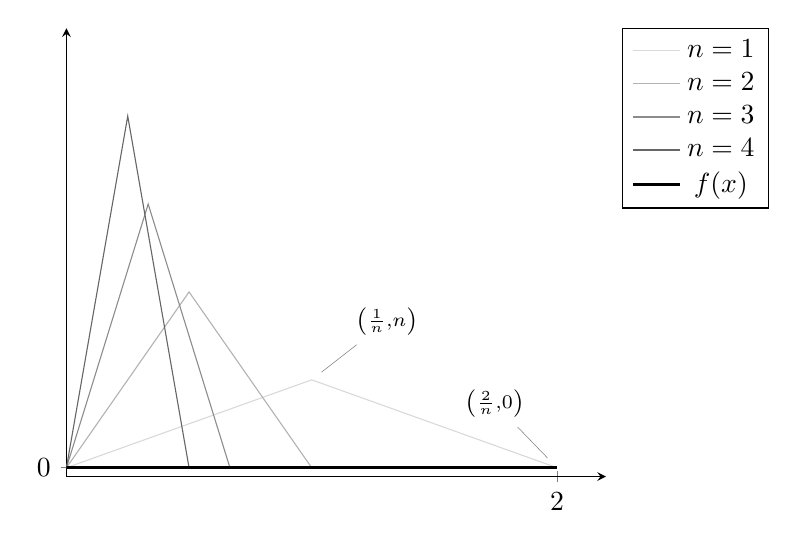
\begin{tikzpicture}
		\begin{axis}[
						enlargelimits,
						legend pos=outer north east,
						axis x line=bottom,axis y line=middle,
						xmin=0,xmax=2.2,ymin=-0.1,ymax=5,ytick={0},xtick={2}
					]
			\addplot [color=black!15!white] coordinates {(0,0) (1/1,1) (2/1,0)};
			\addplot [color=black!30!white] coordinates {(0,0) (1/2,2) (2/2,0)};
			\addplot [color=black!45!white] coordinates {(0,0) (1/3,3) (2/3,0)};
			\addplot [color=black!60!white] coordinates {(0,0) (1/4,4) (2/4,0)};
			\addplot [very thick,color=black,domain=0:2]  {0};
			\node [pin=45:{$\scriptstyle\left(\frac1{n},n\right)$}] at (axis cs:1,1) {};
			\node [pin=120:{$\scriptstyle\left(\frac2{n},0\right)$}] at (axis cs:2,0) {};
			\legend{$n=1$,$n=2$,$n=3$,$n=4$,$f(x)$}
		\end{axis}
	\end{tikzpicture}
	\caption{La successione dell'esempio 3, in $[0,2]$, forma un triangolo di area 1 con l'asse delle ascisse, indipendentemente dal valore di $n$. L'altezza del triangolo aumenta infinitamente al crescere di $n$, mentre la base tende a zero.}
	\label{fig:succ_triangolo}
\end{figure}

\item In $I=[0,1]$, sia
\[
f_n(x)=\begin{cases*}1&se $x=\frac{j}{2^n}$, per $0\leq j\leq 2^n$ intero\\ 0&altrove\end{cases*}.
\]
La funzione limite è la funzione\dots?
\item $f_n(x)=\sqrt{x^2+\frac1{n^2}}$ in $I=\R$, converge puntualmente (figura \ref{fig:succ_iperbole}) alla funzione $f(x)=\abs{x}$.
\begin{figure}
	\tikzsetnextfilename{succ-iperbole}
	\centering
	\begin{tikzpicture}
		\begin{axis}[standard,xtick=\empty,ytick=\empty,xmin=-1.25,xmax=1.25,ymin=-0.5,ymax=2]
			\addplot [samples=500,black!20!white,domain=-1.25:1.25] {sqrt(x^2+1)};
			\addplot [samples=500,black!40!white,domain=-1.25:1.25] {sqrt((x^2)+(1/4))};
			\addplot [samples=500,black!60!white,domain=-1.25:1.25] {sqrt((x^2)+(1/16))};
			\addplot [samples=500,black!80!white,domain=-1.25:1.25] {sqrt((x^2)+(1/36))};
			\addplot [samples=500,black,domain=-1.25:1.25] {abs(x)};
			\node [pin=60:{$\scriptstyle\left(\frac1{n},0\right)$}] at (axis cs:0,1) {};
		\end{axis}
	\end{tikzpicture}
	\caption{Convergenza della funzione $f(x)=\sqrt{x^2+\frac1{n^2}}$ alla funzione limite $f(x)=\abs{x}$, per $n=1,2,4,6$.}
	\label{fig:succ_iperbole}
\end{figure}

\end{enumerate}
Si può studiare se le proprietà della famiglia di funzioni vengano ``ereditate'' dalla funzione limite tramite la convergenza puntuale, ad esempio:
\begin{itemize}
\item se $f_n$ è limitata in $J$ per ogni $n\in\N$, allora anche $f$ è limitata in $J$;
\item se per $\tilde{x}\in J$ esiste il limite delle $f_n(x)$ per $x\to\tilde{x}$, allora $\exists\lim_{x\to\tilde{x}}f(x)$;
\item ulteriormente, per $\tilde{x}\in J$, $\lim_{n\to+\infty}\left(\lim_{x\to\tilde{x}}f_n(x)\right)=\lim_{x\to\tilde{x}}f(x)$;
\item se $f_n$ è continua in $J$ per ogni $n\in\N$, anche $f$ è continua in $J$;
\item se $f_n\in\rie{[a,b]}$ $\forall n\in\N$, allora lo è anche $f$, quando ovviamente $f_n\to f$ in $[a,b]$ e, nel caso, valga
\[
\lim_{n\to+\infty}\int_a^bf_n(x)\,\dd x=\int_a^bf(x)\,\dd x;
\]
\item se ogni $f_n$ è derivabile in $x_0\in J$, allora lo è anche $f$ e, nel caso, valga
\[
\lim_{n\to+\infty}f_n'(x_0)=\left(\lim_{n\to+\infty}f_n\right)'(x_0).
\]
\end{itemize}
Nessuna di queste proprietà è valida: gli esempi elencati precedenti forniscono dei buoni controesempi. La funzione limite del punto 1 è illimitata nell'intervallo considerato, mentre le $f_n$ sono limitate per ogni $n$; nel punto 2, la funzione limite non è continua quando tutte le $f_n$ lo sono; nel punto 3, la $f$ tende a 0 per $x\to+\infty$, diversamente dalle $f_n$ che tendono a 1, $\forall n$; nel punto 5 la $f$ non è integrabile secondo Riemann, mentre lo sono tutte le $f_n$, e il punto 4 mostra che l'integrale di tutte le $f_n$ è 1 (geometricamente, è l'area del triangolo formato dalla curva), mentre quello della $f$ è nullo; nel punto 6 infine ogni $f_n$ ha derivata nulla in $x=0$, ma la funzione limite non è nemmeno derivabile in tale punto.

Per garantire queste proprietà, la convergenza puntuale della successione chiaramente non basta: bisogna introdurre un nuovo tipo di convergenza, detta \emph{uniforme}.
\begin{definizione} \label{d:conv_uniforme_succ}
La successione $\{f_n\}$ converge uniformemente alla funzione limite $f$ in $J$ se
\begin{equation} \label{eq:conv_uniforme_succ}
\forall\epsilon>0,\ \exists\overline{n}=\overline{n}(\epsilon)\colon\forall x\in J,\ \forall n\geq\overline{n}\ \abs{f_n(x)-f(x)}<\epsilon.
\end{equation}
\end{definizione}
La definizione è simile a quella della convergenza puntuale se non per il fatto che la scelta di $\overline{n}$ è ora svincolata dal punto $x\in J$, ma è globale in tutto l'insieme $J$; di conseguenza la convergenza uniforme deve sempre essere associata all'insieme in cui accade. Ovviamente la convergenza uniforme implica automaticamente quella puntuale.
Inoltre la differenza tra $f_n$ e la $f$ è certamente, in modulo, sempre minore del suo estremo superiore in $J$, ossia vale sempre $\abs{f_n(x)-f(x)}\leq\sup_{x\in J}\abs{f_n(x)-f(x)}$. Allora per valutare la convergenza uniforme in $J$ è sufficiente calcolare questo estremo superiore, che dovrà annullarsi. Se infatti per la convergenza puntuale doveva verificarsi $\sup_{x\in J}\lim_{n\to+\infty}\abs{f_n(x)-f(x)}=0$, per la convergenza uniforme si ha che
\begin{equation}
\lim_{n\to+\infty}\sup_{x\in J}\abs{f_n(x)-f(x)}=0.
\end{equation}
Si può anche indicare questo estremo superiore con la \emph{norma uniforme}:
\[
\norm{f_n-f}_{\infty,J}=\sup_{x\in J}\abs{f_n(x)-f(x)}.
\]
\paragraph{Esempi}
\begin{itemize}
\item La successione già vista precedentemente $f_n(x)=x^n$ in $[0,1]$ converge puntualmente, però la $\norm{f_n-f}_{\infty,[0,1]}$ vale 0 in $x=1$, perché $f_n(1)=f(1)$, mentre altrove
\[
\norm{f_n-f}_{\infty,[0,1)}=\sup_{0\leq x<1} x^n=\lim_{x\to 1}x^n=1,
\]
e chiaramente $\lim_{n\to+\infty}\neq 0$ quindi la convergenza non è uniforme. Per $\delta>0$ abritrariamente piccolo, però, considerando non più $[0,1]$ ma $[0,1-\delta]$, si ha che 
\[
\norm{f_n-f}_{\infty,[0,1-\delta]}=\sup_{0\leq x\leq 1-\delta} x^n=(1-\delta)^n\to 0,
\]
per $n\to+\infty$, perciò la convergenza è uniforme, dato che $1-\delta$ non dipende nemmeno più da $x$.
\item La successione
\[
f_n(x)=\frac{\arctan\frac{x}{n}}{1+x^2}
\]
converge puntualmente alla funzione identicamente nulla in $\R$. Sia la funzione limite che i termini della successione sono funzioni dispari, quindi si può studiare la convergenza uniforme anche solo per $x\geq 0$. Risulta:
\[
	\sup_{x\geq 0}\abs[\bigg]{\frac{\arctan\frac{x}{n}}{1+x^2}}\leq\sup_{x\geq 0}\frac{x}{n}\frac1{1+x^2}=\frac1{n}\sup_{x\geq 0}\frac{x}{1+x^2},
\]
poiché l'arcotangente è in modulo sempre minore del suo argomento, inoltre il termine $1/n$ non dipende da $x$ quindi può essere estratto dall'argomento dell'estremo superiore. La funzione $g(x)=\frac{x}{1+x^2}$ è limitata in $\R$, di conseguenza esiste un numero $c\in\R$ per cui $\abs{g(x)}\leq c$, $\forall x\geq 0$. Dunque
\[
\frac1{n}\sup_{x\geq 0}\frac{x}{1+x^2}\leq\frac{c}{n}
\]
che tende a 0 per $n\to+\infty$, quindi la convergenza è uniforme in tutto $\R$.
\item La convergenza della successione
\[
f_n(x)=\frac{\arctan(nx)}{1+x^2}\quad\to\quad\begin{dcases}\frac{\pi}2\frac{\sgn x}{1+x^2}&x\neq 0\\ 0&x=0\end{dcases}
\]
non è uniforme su tutto $\R$, ma lo è in ogni insieme $A\subset\R\setminus[-\epsilon,\epsilon]$, con $\epsilon>0$, ossia escludendo un intorno dell'origine. Infatti
\begin{multline*}
	\sup_{x\geq\epsilon>0}\abs[\bigg]{\frac{\arctan(nx)-\frac{\pi}2\sgn x}{1+x^2}}=\sup_{x\geq\epsilon>0}\frac{\frac{\pi}2-\arctan(nx)}{1+x^2}=\\
=\sup_{x\geq\epsilon>0}\frac{\arctan\frac1{nx}}{1+x^2}=\frac1{1+\epsilon^2}\arctan\frac1{n\epsilon}\to 0
\end{multline*}
per $n\to+\infty$; un risultato analogo si ha per simmetria per $x\leq -\epsilon<0$.
\end{itemize}
Poiché le successioni di funzioni sono comprese in uno spazio metrico completo, quello delle funzioni limitate con la distanza data dalla norma uniforme, in esso si può elaborare la condizione di Cauchy anche per le successioni di funzioni, che sarà sufficiente e necessaria per la convergenza uniforme (dato che la convergenza in tale spazio coincide proprio con la convergenza uniforme)\footnote{Vedere il capitolo \ref{sec:spazi-funz} sugli spazi funzionali.}.
\begin{teorema}
Sia $\{f_n\}$ con $f_n\colon J\to\R$ una successione di funzioni: essa converge uniformemente a $f$ in $J$ se e solo se $\forall\epsilon>0$ $\exists\overline{n}\colon\forall m,n\geq\overline{n}$ si ha $\norm{f_m-f_n}_{\infty,J}<\epsilon$.
\end{teorema}

\section{Proprietà della funzione limite}
Quando la convergenza è uniforme, la funzione limite eredita alcune importanti proprietà dai termini della successione, come mostrato nei seguenti teoremi.
\begin{teorema} \label{t:unif_limitata}
Sia $\{f_n\}$ una successione di funzioni convergente uniformemente a $f$ in $J$ tale che per ogni $n$, $f_n$ è limitata in $J$. Allora anche $f$ è limitata in $J$.
\end{teorema}
\begin{proof}
Se ogni $f_n$ è limitata, vale $\forall n$ che $\abs{f_n(x)}\leq M$.
Per la disuguaglianza triangolare vale inoltre
\[
\abs{f(x)}\leq\abs{f(x)-f_n(x)}+\abs{f_n(x)}\leq\norm{f-f_n}_{\infty,J}+\norm{f_n}_{\infty,J}.
\]
Fissato un $\epsilon>0$ arbitrario, esiste $\overline{n}$ tale per cui $\forall n\geq\overline{n}$, $\norm{f_n-f}_{\infty,J}<\epsilon$. Allora
\[
\sup_{x\in J}\abs{f(x)}\leq\epsilon+\norm{f_{\overline n}}_{\infty,J}.
\]
Poiché il secondo membro è limitato, essendo composto da termini definiti (reali), anche il primo membro è finito, quindi $f(x)$ è limitata in $J$.
\end{proof}
\begin{teorema} \label{t:continuita_conv_uniforme}
Sia $\{f_n\}$ una successione di funzioni definite da $J$ in $\R$, e $x_0\in J$. Se $f_n$ è continua in $x_0$ per ogni $n$, e $\{f_n\}$ converge uniformemente a $f$ in $J$, allora $f$ è a sua volta continua in $x_0$.
\end{teorema}
\begin{proof}
	Per $x\in J$ qualunque, vale la relazione
	\begin{equation}
		\abs{f(x)-f(x_0)}\leq\abs{f_n(x)-f(x)}+\abs{f_n(x)-f_n(x_0)}+\abs{f_n(x_0)-f(x_0)}.
	\end{equation}
	Poiché la convergenza è uniforme, fissato un $\epsilon>0$ esiste $\overline{n}$ per cui $\forall n\geq\overline{n}$ si ha $\norm{f_n-f}_{\infty,J}<\epsilon$, cioè $\abs{f_n(t)-f(t)}<\epsilon$ per ogni $t\in J$; quindi vale anche per i punti $x_0$ e $x$ nella prima equazione. Preso dunque un valore di $n\geq\overline{n}$, ad esempio proprio $\overline{n}$, si ha quindi
	\begin{equation}
		\abs{f(x)-f(x_0)}\leq\epsilon+\abs{f_{\overline n}(x)-f_{\overline n}(x_0)}+\epsilon=\abs{f_{\overline n}(x)-f_{\overline n}(x_0)}+2\epsilon.
	\end{equation}
	La singola funzione $f_{\overline n}(x)$ è continua, per le ipotesi, in $x_0$, quindi in un intorno di tale punto esiste $\delta>0$ tale che per ogni $x\in(x_0-\delta,x_0+\delta)$ si ha $\abs{f_{\overline n}(x)-f_{\overline n}(x_0)}<\epsilon$.
	Allora in tale intorno si ha $\abs{f(x)-f(x_0)}<3\epsilon$, quindi la funzione limite è continua.
\end{proof}
\begin{teorema}[del doppio limite] \label{t:doppio_limite}
Sia $\{f_n\}$ una successione di funzione definite da $J$ a $\R$, e $x_0\in J'$. Se per ogni $n$ esiste $\lim_{x\to x_0}f_n(x)=\ell_n\in\R$, e $\{f_n\}$ converge a $f$ uniformemente in $J$, allora esiste anche $\lim_{n\to+\infty}\ell_n$, che è finito, e coincide con $\lim_{x\to x_0}f(x)$, ossia
\begin{equation} \label{eq:doppio_limite}
\lim_{n\to+\infty}\Big(\lim_{x\to x_0}f_n(x)\Big)=\lim_{x\to x_0}\Big(\lim_{n\to+\infty}f_n(x)\Big).
\end{equation}
\end{teorema}
\begin{teorema} \label{t:scambio_integrale_limite}
Sia $\{f_n\}$ una successione di funzioni definite da $[a,b]$ a $\R$, in cui $f_n$ è integrabile secondo Riemann in $[a,b]$ per ogni $n$, e che converge uniformemente alla funzione $f$ nel medesimo intervallo. Allora anche $f\in\rie{[a,b]}$, e vale
\begin{equation} \label{eq:scambio_integrale_limite}
\lim_{n\to+\infty}\int_a^bf_n(x)\,\dd x=\int_a^b\lim_{n\to+\infty}f_n(x)\,\dd x.
\end{equation}
\end{teorema}
La dimostrazione di questo teorema è piuttosto complicata%?
, quindi se ne dimostra una versione più semplice nel corollario seguente.
\begin{corollario}
Sia $\{f_n\}$ una successione di funzioni definite da $[a,b]$ a $\R$, in cui $f_n$ è continua in $[a,b]$ per ogni $n$, e che converge uniformemente alla funzione $f$ nel medesimo intervallo. Allora vale la \eqref{eq:scambio_integrale_limite}.
\end{corollario}
\begin{proof}
Poiché $f_n\in\cont{[a,b]}$ per ogni $n$, dal teorema \ref{t:continuita_conv_uniforme} segue che anche $f$ lo è, dunque $f\in\rie{[a,b]}$. Inoltre si ha
\begin{multline*}
	\abs[\bigg]{\int_a^bf_n(x)\,\dd x-\int_a^bf(x)\,\dd x}=\abs[\bigg]{\int_a^b\big[f_n(x)-f(x)\big]\,\dd x}\leq\int_a^b\abs{f_n(x)-f(x)}\,\dd x\leq\\
\leq\int_a^b\norm{f_n-f}_{\infty,[a,b]}\,\dd x=\norm{f_n-f}_{\infty,[a,b]}\int_a^b\dd x=(b-a)\norm{f_n-f}_{\infty,[a,b]},
\end{multline*}
che tende a 0 per $n\to+\infty$, e si ha dunque la \eqref{eq:scambio_integrale_limite}.
\end{proof}
Il teorema non è estendibile a insiemi di integrazione illimitati, come mostrato nel seguente esempio: la successione
\[
f_n(x)=\begin{cases}\frac2{n}-\frac2{n^2}x&x<n\\0&x\geq n\end{cases}
\]
converge uniformemente alla funzione $f(x)=0$ (figura \ref{fig:succ_integrazione_illimitata}). L'integrale di ogni $f_n(x)$ in $[0,+\infty)$ vale 1, per ogni $n$, poiché la curva descritta dalla funzione è un triangolo di base $n$ e altezza $2/n$, ma l'integrale della funzione limite è chiaramente nullo.
\begin{figure}
	\tikzsetnextfilename{succ-integrazione-illimitata}
	\centering
	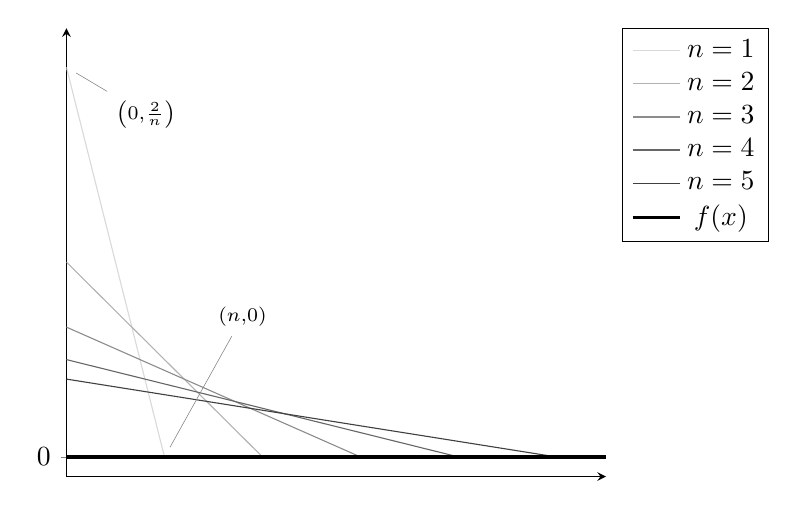
\begin{tikzpicture}
		\begin{axis}[
						enlargelimits,
						legend pos=outer north east,
						axis x line=bottom,axis y line=middle,
						xmin=0,xmax=5.5,ymin=-0.1,ymax=2.2,ytick={0},xtick=\empty
					]
			\addplot [color=black!15!white] coordinates {(0,2/1) (1,0)};
			\addplot [color=black!30!white] coordinates {(0,2/2) (2,0)};
			\addplot [color=black!45!white] coordinates {(0,2/3) (3,0)};
			\addplot [color=black!60!white] coordinates {(0,2/4) (4,0)};
			\addplot [color=black!75!white] coordinates {(0,2/5) (5,0)};
			\addplot [very thick,color=black,domain=0:5.5]  {0};
			\node [pin=-30:{$\scriptstyle\left(0,\frac2{n}\right)$}] at (axis cs:0,2) {};
			\node [pin={[pin distance=1.5 cm]70:{$\scriptstyle(n,0)$}}] at (axis cs:1,0) {};
			\legend{$n=1$,$n=2$,$n=3$,$n=4$,$n=5$,$f(x)$}
		\end{axis}
	\end{tikzpicture}
	\caption{La successione $f_n(x)=\frac2{n}-\frac2{n^2}x$ per $x<n$ e $f_n(x)=0$ per $x\geq n$ forma un triangolo di area 1 con gli assi cartesiani, indipendentemente dal valore di $n$.}
	\label{fig:succ_integrazione_illimitata}
\end{figure}


La derivabilità di una successione di funzioni è una questione più complicata dell'integrabilità: si è già visto in un precedente esempio che anche se la successione converge uniformemente, non è sempre vero che converge anche la successione delle derivate, come per $f_n(x)=\sqrt{x^2+\frac1{n^2}}$, la cui derivata della funzione limite non esiste nemmeno, in $x=0$.
\begin{teorema} \label{t:scambio_derivata_limite}
Sia $\{f_n\}$ una successione di funzioni definite da $[a,b]$ in $\R$ e derivabili in tale intervallo. Se esiste un punto $x_0\in[a,b]$ per cui $\{f_n(x_0)\}$ converge, e se la successione delle derivate $\{f_n'\}$ converge uniformemente in $[a,b]$ ad una funzione $g$, allora esiste una funzione $f\colon[a,b]\to\R$ derivabile, tale che
\begin{itemize}
\item $\{f_n\}$ converga uniformemente a $f$ in $[a,b]$;
\item $f'(x)=g(x)$ in ogni punto $x\in[a,b]$, ossia
\[
\lim_{n\to+\infty}f'_n(x)=\Big(\lim_{n\to+\infty}f_n\Big)'(x).
\]
\end{itemize}
\end{teorema}
Si dà la dimostrazione nel caso particolare in cui $f_n\in\cont[1]{[a,b]}$, per ogni $n$.
\begin{proof}
Poiché $f_n'\in\cont{[a,b]}$, anche $g$ lo è per il teorema \ref{t:continuita_conv_uniforme}. Sapendo che esiste ed è finito il limite
\[
\lim_{n\to+\infty}f_n(x_0)=f(x_0),
\]
si costruisce per ogni punto $x\in[a,b]$ la funzione
\[
f(x)=f(x_0)+\int_{x_0}^xg(t)\,\dd t.
\]
Essa è derivabile, poiché l'integranda $g$ è continua, $f$ è derivabile per il teorema fondamentale del calcolo integrale \ref{t:tfci1} e la sua derivata è $f'(x)=g(x)$ in $[a,b]$. Inoltre per il medesimo teorema si ha $f_n(x)=f_n(x_0)+\int_{x_0}^xf_n'(t)\,\dd t$, quindi $\forall x\in[a,b]$ risulta
\[\begin{split}
\abs{f(x)-f_n(x)}	&=\abs{f(x_0)+\int_{x_0}^xg(t)\,\dd t-f_n(x_0)-\int_{x_0}^xf_n'(t)\,\dd t}\leq\\
				&\leq\abs{f(x_0)-f_n(x_0)}+\abs{\int_{x_0}^x\big[g(t)-f_n'(t)\big]\,\dd t}\leq\\
				&\leq\abs{f(x_0)-f_n(x_0)}+\abs{x-x_0}\norm{g-f_n'}_{\infty,[a,b]}\leq\\
				&\leq\abs{f(x_0)-f_n(x_0)}+(b-a)\norm{g-f_n'}_{\infty,[a,b]},
\end{split}\]
e poiché per le ipotesi $f_n(x_0)\to f(x_0)$ per $n\to+\infty$, ed $\{f_n'\}$ converge a $g$, si ha che $\{f_n\}$ converge a $f$; la convergenza è infine uniforme in quanto non dipende affatto dalla scelta di $x$, come si nota nell'ultima riga dell'equazione dove la variabile non compare più.
\end{proof}
È importante che la successione $\{f_n\}$ converga almeno in un punto: se si guarda alla successione $f_n(x)=n$, che è costante, la successione delle derivate è $f_n'(x)=0$, cioè sono tutte identicamente nulle ($f_n$ infatti è costante), quindi ovviamente $\{f_n'\}$ converge uniformemente alla funzione identicamente nulla. Ma si nota facilmente che $f_n$ non converge in nessun punto dell'asse reale, nemmeno puntualmente, quindi non esistono nemmeno la funzione limite $f$ né la sua derivata $f'$.

\section{Spazi funzionali}
\label{sec:spazi-funz}
Si indica con la scrittura $\bounded[F]{E}$, dove $E\subseteq\R^m$ e $F\subset\R^p$ è chiuso, l'insieme delle funzioni definite in $E$ a valori in $F$ che sono limitate. Su tale insieme si può costruire una struttura spazio metrico, introducendo la distanza
\[
d(\vec f,\vec g)=\sup_{\vec x\in E}\norm{\vec f(\vec x)-\vec g(\vec x)}_F,
\]
dove $\norm{\cdot}_F$ è la norma euclidea in $\R^p$. È un'operazione binaria definita come $d\colon\bounded[F]{E}\times\bounded[F]{E}\to\R$.
Tale distanza è ben definita, perché tutte le $p$ componenti di $\vec f$ e $\vec g$ sono limitate, quindi $\norm{\vec f(\vec x)}_F\leq M$ e $\norm{\vec g(\vec x)}_F\leq K$ $\forall\vec x\in E$, quindi per la disuguaglianza triangolare risulta $\norm{\vec f(\vec x)-\vec g(\vec x)}_F\leq M+K$, cioè $d(\vec f,\vec g)\leq M+K<+\infty$.
Inoltre soddisfa le proprietà che definiscono una distanza, ossia:
\begin{itemize}
	\item $d(\vec f,\vec g)\ge 0$ $\forall\vec x\in E$ in quanto è una norma euclidea, e $d(\vec f,\vec g)=0$ se e solo se $\norm{\vec f(\vec x)-\vec g(\vec x)}_F=0$ per ogni punto $\vec x\in E$, vale a dire che per tutti i punti $\vec x_0\in E$ risulta $\vec f(\vec x_0)=\vec g(\vec x_0)$, cioè le funzioni coincidono.
	\item $d(\vec f,\vec g)=d(\vec g,\vec f)$ per la simmetria della norma euclidea.
	\item Date tre funzioni $\vec f,\vec g,\vec h\in\bounded[F]{E}$, per la disuguaglianza triangolare della norma euclidea si ha
	\begin{equation}
		\begin{split}
			\norm{\vec f(\vec x)-\vec g(\vec x)}_F&\leq\norm{\vec f(\vec x)-\vec h(\vec x)+\vec h(\vec x)-\vec g(\vec x)}_F\leq\\
			&\leq\norm{\vec f(\vec x)-\vec h(\vec x)}_F+\norm{\vec h(\vec x)-\vec g(\vec x)}_F\leq\\
			&\leq d(\vec f,\vec h)+d(\vec h,\vec g).
		\end{split}
	\end{equation}
Poiché quindi per ogni punto $\vec x\in E$ la norma $\norm{\vec f(\vec x)-\vec g(\vec x)}_F$ non supera questa somma delle distanze, anche il suo estremo superiore non la potrà superare, dunque
\[
\sup_{\vec x\in E}\norm{\vec f(\vec x)-\vec g(\vec x)}_F=d(\vec f,\vec g)\leq d(\vec f,\vec h)+d(\vec h,\vec g).
\]
\end{itemize}
Lo spazio $\bounded[F]{E}$ può assumere anche la struttura di spazio vettoriale, a seconda che lo sia prima l'insieme $F$ di arrivo. Infatti per la disuguaglianza triangolare la somma di due funzioni limitate è limitata, e analogamente per il prodotto con uno scalare di una funzione limitata. Le immagini dei risultati di queste due operazioni però non appartengono necessariamente ad $F$: questo accade soltanto se l'insieme $F$ è a sua volta uno spazio vettoriale.

Data una successione di funzioni $\vec f_n$ convergente alla funzione limite $\vec f$, secondo tale metrica la convergenza accade se $d(\vec f_n,\vec f)\to 0$ per $n\to+\infty$, cioè se $\vec f_n$ converge uniformemente a $\vec f$.
\begin{teorema}
$\bounded[F]{E}$ è uno spazio metrico completo.
\end{teorema}
\begin{proof}
Una successione $\{\vec f_n\}_{n\in\N}$ soddisfa la condizione di Cauchy rispetto alla distanza $d$ se $\forall\epsilon>0$, $\exists N=N(\epsilon)\colon\forall m,n\geq N$ si ha $d(\vec f_n,\vec f_m)<\epsilon$, cioè
\[
\sup_{\vec x\in E}\norm{\vec f_n(\vec x)-\vec f_m(\vec x)}_F<\epsilon,
\]
cioè se e solo se soddisfa il criterio di Cauchy per la convergenza uniforme, quindi $\exists\vec f\colon E\to F$ tale che $\vec f_n\to \vec f$ uniformemente in $E$. Allora $\vec f$ è anche limitata, cioè appartiene a $\bounded[F]{E}$.
\end{proof}
Più in generale la funzione limite $\vec f$ avrebbe valori nella chiusura di $F$, ma essa coincide con $F$ stesso poiché è chiuso. Le proprietà dello spazio $\bounded[F]{E}$ dipendono fortemente quindi dalla completezza di $F$.

\subsection*{Spazio delle funzioni continue}
% Ridefinisco temporaneamente per questa sezione il comando per le funzioni continue
\renewcommand{\cont}[2][]{\mathscr C^{#1}_{#2}\parentheses} % Uso: \cont[k]{A}{B} equivale a C^k_B(A), per f:A->B
%
Siano $E\subset\R^n$ un insieme compatto e $F\subset\R^p$ chiuso. La scrittura $\cont{E}{F}$, o anche $\cont[0]{E}{F}$, individua lo spazio delle funzioni continue definite da $E$ a $F$.
Per il teorema \ref{t:weierstrass} di Weiestra\ss, tutte le $\vec f\in\cont[0]{E}{F}$ sono limitate perché $E$ è compatto, quindi $\cont[0]{E}{F}\subset\bounded[F]{E}$.

Con la distanza $d$ definita per le funzioni limitate, anche $(\cont[0]{E}{F},d)$ è uno spazio metrico, ed è anch'esso completo, perché per il teorema \ref{t:continuita_conv_uniforme}, se per ogni $n\in\N$ le funzioni $\vec f_n$ sono continue, allora quando $d(\vec f_n,\vec f)\to 0$ significa che la successione converge uniformemente a $\vec f$, che quindi eredita la continuità; allora se $\{\vec f_n\}_{n\in\N}$ soddisfa la condizione di Cauchy, essa converge in $\cont[0]{E}{F}$.
%
\renewcommand{\cont}[1][]{\mathscr C^{#1}\parentheses} % Torna come prima

\section{Teorema delle contrazioni}
\begin{definizione}
Dato uno spazio metrico $(X,d)$ e una funzione $T\colon(X,d)\to(X,d)$, $T$ si dice \emph{contrazione} se esiste un valore $k\in[0,1)$ tale per cui
\[
d\big(T(x)-T(y)\big)\leq k d(x,y)
\]
per ogni coppia $x,y\in X$, ossia se $T$ ``contrae'' le distanze (anche non uniformemente) tra $x$ e $y$.
\end{definizione}
Una contrazione è sempre, come si nota facilmente, una funzione lipschitziana di costante $k<1$, quindi è uniformemente continua.
\begin{teorema}[di Banach-Caccioppoli] \label{t:contrazioni}
Sia $(X,d)$ uno spazio metrico completo, e $T\colon X\to X$ una contrazione su $X$. Allora esiste, ed è unico, un \emph{punto fisso} $x^*\in X$ tale per cui $T(x^*)=x^*$.
\end{teorema}
\begin{proof}
Sia $x_0\in X$, $x_1$ l'immagine di $x_0$ attraverso la contrazione $T$ e così via seguendo la regola $x_n=T(x_{n-1})$, per ogni $n\in\N_0$. La distanza tra due elementi della successione costruita in questo modo è
\begin{equation*}
d(x_{n+1},x_n)=d\big(T(x_n),T(x_{n-1})\big)\leq kd(x_n,x_{n-1})\leq k^2d(x_{n-1},x_{n-2})\leq\dots\leq k^nd(x_1,x_0).
\end{equation*}
Dati $m$ e $n$, con $m>n$, si ha per la disguaglianza triangolare che
\begin{equation}
\begin{split}
d(x_m,x_n)\leq	&d(x_m,x_{m-1})+d(x_{m-1},x_{m-2})+\dots+d(x_{n+1},x_n)=\\
				&=\sum_{i=n}^{m-1}d(x_{i+1},x_i)\leq\sum_{i=n}^{m-1}k^id(x_1,x_0)=\\
				&=d(x_1,x_0)k^n\sum_{i=n}^{m-1}k^{i-n}=d(x_1,x_0)k^n\sum_{j=0}^{m-n-1}k^j
\end{split}
\end{equation}
e si ha che
\[
\sum_{j=0}^{m-n-1}k^j\leq\sum_{j=1}^{+\infty}k^j=\frac1{1-k},
\]
quindi risulta
\begin{equation}
d(x_m,x_n)\leq\frac{k^n}{1-k}d(x_1,x_0).
\end{equation}
Allora, poiché $k<1$, il secondo termine tende a 0 quindi $\forall\epsilon>0$ $\exists\overline{n}\colon\forall m>n\geq\overline{n}$ si ha $d(x_m,x_n)<\epsilon$, ossia la successione soddisfa la condizione di Cauchy. Dato che lo spazio metrico $(X,d)$ è completo, $\{x_n\}$ converge ad un punto $x^*\in X$ per $n\to+\infty$.
La contrazione $T$ è infine (uniformemente) continua, quindi
\[
T(x^*)=T\Big(\lim_{n\to+\infty}x_n\Big)=\lim_{n\to+\infty} T(x_n)=\lim_{n\to+\infty} x_{n+1}=x^*,
\]
quindi $x^*$ è un punto fisso di $T$; per l'unicità del limite (teorema \ref{t:unicita_limite}) è inoltre unico.
\end{proof}
Non rispettando le ipotesi il teorema non è sempre ancora valido, come ad esempio nello spazio $\R\setminus\{0\}$ con la distanza euclidea: la funzione $f(x)=\frac{x}2$ è una contrazione, ma il suo punto fisso, che sarebbe $x=0$, non appartiene allo spazio.
Anche se $T$ non è una contrazione si hanno degli effetti indesiderati: se $k=1$, infatti le distanze rimangono costanti, come per $g(x)=x+1$, che non ha punti fissi, o per $h(x)=x$ che ne ha infiniti.
\begin{osservazione}
Il teorema \ref{t:contrazioni} non vale se la funzione $T$ è tale per cui $d\big(T(x),T(y)\big)<d(x,y)$, ossia con una disuguaglianza stretta. Infatti, sia $X=[1,+\infty)$: la funzione $f(x)=x+\frac1{x}$ soddisfa questa condizione, ma non ha punti fissi.
\end{osservazione}

\chapter{Serie di funzioni}
Analogamente alle serie numeriche, si può costruire una successione di somme parziali a partire da una successione di funzioni. Sia $\{f_n(x)\}$, con $n\in\N_0$ o un opportuno sottoinsieme, una successione di funzioni definite tutte su un medesimo insieme $E$; si consideri la successione $S_k(x)$ come la somma dei primi $k$ termini di $\{f_n(x)\}$
\[
S_n(x)=\sum_{n=1}^kf_n(x),
\]
ovviamente sempre definita in $E$: essa è la successione delle somme parziali.
La serie di funzioni
\[
S(x)=\ser{n}f_n(x)
\]
converge in $x_0$ se converge la serie numerica $\ser{n}f_n(x_0)$. La funzione $S(x)$, definita ovunque la serie di funzioni converga, è anche chiamata \emph{funzione somma}.

\section{Convergenza puntuale e uniforme}
Unendo la teoria delle serie numeriche con quella delle successioni di funzioni si ottengono le definizioni seguenti.
\begin{definizione}
La serie $\ser{n}f_n(x)$ converge \emph{puntualmente} in $J\subseteq E$ se $\ser{n}f_n(x_0)$ converge in ogni punto $x_0\in J$.
\end{definizione}
\begin{definizione}
La serie $\ser{n}f_n(x)$ converge \emph{assolutamente} in $J\subseteq E$ se $\ser{n}\abs{f_n(x)}$ converge $\forall x\in J$.
\end{definizione}
\begin{definizione}
La serie $\ser{n}f_n(x)$ converge \emph{uniformemente} in $J\subseteq E$ se la successione $S_k(x)$ converge uniformemente a $S(x)$ in $J$, cioè se
\[
\norm{S_k-S}_{\infty,J}\to 0\quad\text{per }n\to\pinf.
\]
\end{definizione}

Nel capitolo \ref{sec:spazi-funz} si era visto che lo spazo metrico delle funzioni limitate e quello delle funzioni continue $\cont{k}(E)$ sono spazi vettoriali, se si assume come insieme di arrivo l'intero $\R$. Da ciò segue che la funzione somma di funzioni limitate è a sua volta limitata, e analogamente è continua quando è somma di funzioni continue (dello stesso ordine $k$). Dunque la successione $S_k(x)$ delle somme parziali assume le stesse proprietà delle $f_n(x)$ di cui è somma:
\begin{itemize}
\item se $f_n$ è limitata per ogni $n$, allora $S_k$ è limitata;
\item se $f_n\in\cont{p}$ per ogni $n$, allora anche $S_k\in\cont{p}$.
\end{itemize}
Chiaramente la somma (finita) di funzioni limitate o continue è ancora limitata o continua: non sempre lo stesso vale per la funzione somma, per la quale si applica il seguente teorema.
\begin{teorema}
	Se $f_n(x)\in\cont{}(J)$ $\forall n$ e $S(x)=\ser{n}f_n(x)$ converge uniformemente in $J$, allora $S\in\cont{}(J)$.
\end{teorema}
\begin{teorema} \label{t:continuita_serie_conv_uniforme}
Se esiste finito il $\lim_{x\to x_0}f_n(x)=\ell_n\in\R$, per ogni $n$, e $S(x)=\ser{n}f_n(x)$ converge uniformemente in $J$, allora la serie $\ser{n}\ell_n$ converge e vale
\[
\ser{n}\ell_n=\lim_{x\to x_0}S(x)\then\ser{n}\lim_{x\to x_0}f_n(x)=\lim_{x\to x_0}\ser{n}f_n(x).
\]
\end{teorema}
\begin{teorema} \label{t:scambio_integrale_serie}
Se $f_n\in\rie\ab$ per ogni $n$ e la serie $S(x)=\ser{n}f_n(x)$ converge uniformemente in $[a,b]$, allora $S\in\rie\ab$ e vale
\[
\int_a^b\ser{n}f_n(x)\,\dd x=\ser{n}\int_a^bf_n(x)\,\dd x.
\]
\end{teorema}
\begin{teorema} \label{t:scambio_derivata_serie}
Se $f_n(x)$ è derivabile in $[a,b]$ per ogni $n$, la serie delle derivate $\ser{n}f_n'(x)$ converge uniformemente in $[a,b]$, ed esiste un punto $x_0\in[a,b]$ per cui la serie $\ser{n}f_n(x_0)$ converge, allora la serie $\ser{n}f_n(x)$ converge uniformemente in $[a,b]$ e vale
\[
S'(x)=\bigg(\ser{n}f_n(x)\bigg)'=\ser{n}f_n'(x).
\]
\end{teorema}

Poiché la successione delle somme parziali $\{S_k\}$ converge uniformemente in $J$ se e solo se soddisfa la condizione di Cauchy (come per le successioni), cioè se per ogni $\epsilon>0$ esiste in corrispondenza un $\overline{n}(\epsilon)$ tale che per ogni $n>m\geq\overline{n}$ interi si abbia
\[
\norm{S_n-S_m}_{\infty,J}=\bigg\|\sum_{k=m+1}^nf_k\bigg\|_{\infty,J}<\epsilon.
\]
Posti $m+1=p$ e $q>0$, si ottiene che la condizione è soddisfatta se $\forall p>\overline{n}(\epsilon)$ e $q>0$ interi si ha
\begin{equation} \label{eq:cc_serie_funzioni}
\bigg\|\sum_{k=p}^{p+q}f_k(x)\bigg\|_{\infty_J}<\epsilon.
\end{equation}
Da questo si ottiene una condizione necessaria per la convergenza uniforme della serie.
\begin{corollario}
La serie $\ser{n}f_n(x)$ converge uniformemente in $J$ solo se la successione $\{f_n(x)\}$ dei termini generali converge uniformemente in $J$.
\end{corollario}
\begin{proof}
Ponendo $q=0$ nella \eqref{eq:cc_serie_funzioni}, si ottiene che
\[
\bigg\|\sum_{k=p}^{p}f_k(x)\bigg\|_{\infty_J}=\norm{f_p}_{\infty_J}<\epsilon,
\]
ossia che $\forall\epsilon>0$ $\exists\overline{n}(\epsilon)$ tale per cui $\forall p>\overline{n}$ si ha $\norm{f_p-0}_{\infty,J}<\epsilon$ cioè $f_p$ (o equivalentemente $f_n$) converge uniformemente alla funzione identicamente nulla.
\end{proof}
La condizione appena data è ovviamente solamente necessaria: la serie $\ser{n}\frac1{n}$ diverge, ma il suo termine generale $f_n(x)=\frac1{n}$ converge uniformemente alla $f\equiv 0$ in tutto $\R$.

\section{Convergenza totale}
\begin{definizione}
Si dice che la serie $\ser{n}f_n(x)$ converge \emph{totalmente} in $J$ se esiste una successione numerica $\{M_n\}\subset\R$ tale che $\abs{f_n(x)}\leq M_n$ per ogni $n$ e $x\in J$, e per cui la serie $\ser{n}M_n$ converga.
\end{definizione}
La definizione continua a valere se come successione $\{M_n\}$ si prende il minimo dei maggioranti di $f_n(x)$ in $J$, che è proprio la norma uniforme: allora la convergenza é totale anche quando la serie $\ser{n}\norm{f_n}_{\infty,J}$ converge.
\begin{teorema}[di Weierstrass]
Se $\ser{n}f_n(x)$ converge totalmente in $J$, allora converge anche uniformemente.
\end{teorema}
\begin{proof}
Per ipotesi esiste una successione $\{M_n\}$ la cui serie converge e tale che per ogni $n$ si abbia $\norm{f_n}_{\infty,E}\leq M_n$, $\forall x\in E$. Allora la serie $\ser{n}M_n$ soddisfa la condizione di Cauchy: per ogni $\epsilon>0$ esiste $\overline{n}$ tale per cui $\forall p\geq\overline{n}$ e $q>0$ interi si abbia
\[
\sum_{n=p}^{p+q}M_n<\epsilon,
\]
ma allora per le disuguaglianze precedenti risulta
\[
\epsilon>\sum_{n=p}^{p+q}M_n\geq\sum_{n=p}^{p+q}\norm{f_n}_{\infty,E}\geq\bigg\|\sum_{n=p}^{p+q}f_n\bigg\|_{\infty,E}
\]
quindi la serie converge anche uniformemente per le \eqref{eq:cc_serie_funzioni}.
\end{proof}
La convergenza totale implica anche la convergenza assoluta, come è facile vedere. Ovviamente non valgono le implicazioni nel senso inverso: né la convergenza uniforme né quella assoluta, né entrambe (e men che meno quella puntuale) implicano la convergenza totale.
\paragraph{Esempi}
\begin{itemize}
\item La serie $\ser{n}\frac{(-1)^n}{n}$ ha come termine generale una funzione costante, e ovviamente converge puntualmente per il criterio di Leibnitz in tutto $\R$, ma non assolutamente. Non dipendendo in alcun modo dalla variabile $x$, la convergenza è sicuramente anche uniforme.
\item La serie $\ser{n}x^n$ converge puntualmente in $J=(-1,1)$, anche assolutamente essendo a termini positivi, ma non uniformemente perché $\norm{f_n}_{\infty,J}=f_n(1)=1$.
\item Considerata solo in $\R^+$, la serie di termine generale $f_n(x)=\frac1{x}\delta_{[n,n+1]}\scriptstyle(x)$ converge puntualmente ed assolutamente (la somma corrisponde in effetti all'integrale improprio $\int_1^{\pinf}\frac1{x}\,\scriptstyle\dd x$), inoltre $\norm{S-S_n}_{\infty,\R^+}\leq\frac1{n+1}\to 0$, quindi converge uniformemente. La convergenza non è però totale in quanto $\norm{f_n}_{\infty,\R^+}=\frac1{n}$ la cui serie diverge.
\end{itemize}

\section{Serie di potenze}
Le serie di potenze sono un caso particolare e importante di serie di funzioni: dati un punto $x_0\in\R$ e una successione $\{a_n\}\subset\R$, si chiama serie di potenze di centro $x_0$ e coefficiente $a_n$ la serie
\[
\serz{n}a_n(x-x_0)^n.
\]
Qualunque serie di potenze converge sempre in $x_0$, dove il termine generale è sempre nullo: dunque l'insieme di convergenza puntuale non è mai vuoto.
Tutte le serie di potenze saranno indicate in questo capitolo con $n\in\{0,1,\dots\}$, senza perdere la generalità; laddove vi siano problemi di esistenza del coefficiente $a_n$, l'indice iniziale sarà opportunamente cambiato. Ovviamente ciò non cambia il carattere della serie, ma è importante quando si intende calcolare la funzione somma.
Per comodità, tramite la traslazione $y=x-x_0$ si ottiene la serie $\serz{n}a_ny^n$, che è centrata in $y=0$ e mantiene le stesse caratteristiche qualitative della precedente, opportunamente traslate: d'ora in poi si tratteranno soltanto serie di potenze con questa scrittura.
\paragraph{Esempi}
\begin{itemize}
\item La serie $\serz{n}n^nx^n$ converge solo in $x=0$: altrove infatti $\sqrt[n]{n^nx^n}=n\abs{x}\to\pinf$ se $x\neq 0$ quindi diverge per il criterio della radice.
\item $\serz{n}\frac{x^n}{n^n}$, sempre per il criterio della radice, converge puntualmente in tutto $\R$.
\item $\serz{n}x^n$ converge puntualmente in $E=(-1,1)$, ma non uniformemente, perché $\sup_{x\in E}\abs{x^n}=f_n(1)=1^n=1$.
\end{itemize}
\begin{teorema}
Data una serie di potenze $\serz{n}a_nx^n$, se converge puntualmente in $x_0\neq 0$, allora converge assolutamente in tutto l'intervallo $(-\abs{x_0},\abs{x_0})$. La convergenza è inoltre totale, quindi anche uniforme, in ogni sottoinsieme compatto di esso.
\end{teorema}
\begin{proof}
Sia $\serz{n}a_nx^n$ convergente in $\xi\neq 0$: allora necessariamente deve risultare $\abs{a_n\xi^n}\to 0$, quindi esiste $c>0$ tale per cui per ogni $n$ si abbia $\abs{a_n\xi^n}<c$. Allora
\[
\abs{a_nx^n}=\abs{a_n\xi^n}\abs{\frac{x}{\xi}}^n\leq c\abs{\frac{x}{\xi}}^n,
\]
che è il termine generale di una serie geometrica, e converge dunque per $\abs{x/\xi}<1$ cioè per $x\in(-\abs{\xi},\abs{\xi})$. Per il teorema del confronto, $\serz{n}a_nx^n$ converge assolutamente nel medesimo intervallo.
Se poi $K$ è un sottoinsieme compatto di tale intervallo, sicuramente $\abs{x/\xi}\leq 1-\delta$ per qualche $\delta>0$, ma allora $\abs{a_nx^n}\leq c(1-\delta)^n$ quindi $\serz{n}a_nx^n$ converge totalmente.
\end{proof}
\begin{definizione}
Si chiama \emph{raggio di convergenza} di una serie di potenze $\serz{n}a_nx^n$ la quantità
\[
\rho=\sup\bigg\{x\in\R\colon\ser{n}a_nx^n\text{ è convergente}\bigg\}.
\]
\end{definizione}
Il raggio $\rho$ appartiene a $[0,\pinf]$:
\begin{itemize}
\item se $\rho=0$ la serie converge solo in 0;
\item se $\rho\notin\{0,\pinf\}$, la serie converge assolutamente in $(-\rho,\rho)$, totalmente nei sottoinsiemi compatti, non converge se $\abs{x}>\rho$;
\item se $\rho=\pinf$, la serie converge assolutamente $\forall x\in\R$ e totalmente in ogni insieme compatto.
\end{itemize}
Per determinare il raggio di convergenza si ricorre ai criteri seguenti.
Quando $\rho\neq 0$, non si può affermare nulla sul comportamento della serie al bordo di $(-\rho,\rho)$.
\begin{teorema}[Criterio di Cauchy-Hadamard]
Sia $\rho$ il raggio di convergenza della serie $\serz{n}a_nx^n$. Se
\[
\ell=\limsup_{n\to\pinf}\sqrt[n]{\abs{a_n}},
\]
allora $\rho=\frac1{\ell}$, usando l'algebra di $\Rex$.
\end{teorema}
\begin{proof}
Per il criterio \ref{t:criterio_radice_serie} della radice si ha
\[
\limsup_{n\to\pinf}\sqrt[n]{\abs{a_nx^n}}=\abs{x}\limsup_{n\to\pinf}\sqrt[n]{\abs{a_n}}\equiv \abs{x}\ell.
\]
che deve essere minore di 1, quindi $\abs{x}<1/\ell$: allora $\rho=1/\ell$ è il raggio di convergenza.
\end{proof}
Questo criterio è sempre utilizzabile, in quanto il limite superiore di una successione, in $\Rex$, esiste sempre (teorema \ref{t:classe_limite_mai_vuota}).
\begin{teorema}[Criterio di d'Alembert]
Se $a_n\neq 0$ per ogni $n$ ed esiste il limite
\[
\lim_{n\to\pinf}\abs{\frac{a_{n+1}}{a_n}}\equiv\ell,
\]
allora il raggio di convergenza della serie $\serz{n}a_nx^n$ è $\rho=1/\ell$.
\end{teorema}
La dimostrazione è analoga a quella del teorema precedente. Questo criterio inoltre mostra che se $a_n$ ha una crescita o decrescita di tipo polinomiale il raggio di covergenza è 1.
Non è possibile stabilire a priori la convergenza ai bordi dell'intervallo di convergenza, ma il caso va studiato di volta in volta. Ad esempio:
\begin{itemize}
\item la serie $\serz{n}x^n$ converge in $(-1,1)$;
\item la serie $\serz{n}\frac{x^n}{n}$ converge in $[-1,1)$, in $x=-1$ in particolare per il criterio di Leibnitz;
\item la serie $\serz{n}\frac{x^n}{n^2}$ converge in $[-1,1]$.
\end{itemize}

\section{Proprietà delle serie di potenze}
\begin{teorema}
Una serie di potenze è continua nell'intervallo di convergenza $(-\rho,\rho)$.
\end{teorema}
\begin{proof}
In ogni punto $x_0\in(-\rho,\rho)$, si trova un intervallo compatto $[a,b]\subset(-\rho,\rho)$ con $a<x_0<b$. Essendo un insieme compatto, la serie converge totalmente in $[a,b]$, e poiché $a_nx^n$ è continua in $[a,b]$ per ogni $n$ si ha per il teorema \ref{t:continuita_serie_conv_uniforme} che anche la serie è continua in $[a,b]$, quindi in $x_0$.
La serie è quindi continua in tutti i punti $x_0\in(-\rho,\rho)$. 
\end{proof}
\begin{teorema}[di Abel]
Se la serie di potenze $\ser{n}a_nx^n$ ha un raggio di convergenza $\rho$ non nullo e converge in $x=\rho$, allora converge uniformemente nei sottoinsiemi compatti di $(-\rho,\rho]$.
\end{teorema}
La tesi vale ovviamente anhe nel caso in cui la serie converga in $x=-\rho$, per cui la convergenza è uniforme in $[-\rho,\rho)$, o anche entrambi.
Come conseguenza, la serie è anche continua sul bordo di $(-\rho,\rho)$, dove converge: ciò significa che
\[
\lim_{x\to\rho^-}\serz{n}a_nx^n=\serz{n}a_n\rho^n.
\]
È possibile calcolare l'integrale di una serie di potenze trasformandolo in una serie numerica grazie al teorema seguente.
\begin{teorema} \label{t:integrale-serie-potenze}
	Sia $\serz{n}a_nx^n$ con raggio di convergenza $\rho$.
	Per $[\alpha,\beta]\subset(-\rho,\rho)$ vale l'uguaglianza
	\begin{equation}
		\int_\alpha^\beta\serz{n}a_nx^n\,\dd x=\serz{n}a_n\frac{\beta^{n+1}-\alpha^{n+1}}{n+1}.
	\end{equation}
\end{teorema}
\begin{proof}
	L'intervallo $[\alpha,\beta]$ è un sottoinsieme compatto dell'intervallo di convergenza, in cui quindi la serie converge uniformemente, e il termine $a_nx^n$ è certamente integrabile secondo Riemann.
	È quindi possibile applicare il teorema \ref{t:scambio_integrale_serie} che permette di scambiare l'ordine di serie ed integrale.
	Integrando la serie termine a termine si ottiene
	\begin{equation}
		\int_\alpha^\beta\serz{n}a_nx^n\,\dd x=\serz{n}\int_\alpha^\beta a_nx^n\,\dd x=\serz{n}a_n\int_\alpha^\beta x^n\,\dd x=\serz{n}a_n\frac{\beta^{n+1}-\alpha^{n+1}}{n+1}.
	\end{equation}
\end{proof}

Dove la convergenza è uniforme, si può calcolare la derivata di una serie di potenze termine a termine: la derivata di $\serz{n}a_nx^n$ è dunque
\[
\serz{n}na_nx^{n-1}.
\]
Dato che il primo termine, corrispondente a $n=0$, è costante (vale $a_0$) la sua derivata è nulla, quindi non appare nella serie derivata; si può allora trascurare, senza alterare in alcun modo la serie, il primo termine facendo partire la serie da $n=1$, ottenendo
\[
\ser{n}na_nx^{n-1}.
\]
Scalando gli indici di 1 si riscrive quindi la serie derivata come
\[
\serz{n}(n+1)a_{n+1}x^n.
\]
Si calcola ora il suo raggio di convergenza $\rho'$, con il limite
\[
\sqrt[n]{(n+1)\abs{a_{n+1}}}=\sqrt[n]{n+1}\sqrt[n+1]{\abs{a_{n+1}}}^{\frac{n+1}{n}}.
\]
Il termine $\sqrt[n]{n+1}$ tende a 1, così come l'esponente $\frac{n+1}{n}$ nella seconda radice. Il termine $\sqrt[n+1]{\abs{a_{n+1}}}$ al limite per $n\to\pinf$ tende a $1/\rho$ dove $\rho$ è lo stesso raggio di convergenza della serie primitiva. Quindi si può formulare il teorema seguente.
\begin{teorema}
Sia $S(x)$ la funzione somma della serie $\serz{n}a_nx^n$, con raggio di convergenza non nullo: $S$ è derivabile in $(-\rho,\rho)$ e vale
\[
S'(x)=\serz{n}(n+1)a_{n+1}x^n,
\]
con lo stesso raggio di convergenza di $S(x)$.
\end{teorema}
\begin{proof}
La serie $\serz{n}a_nx^n$ ha come termine generale una funzione continua e derivabile per ogni $n$, e converge sicuramente in $x=0$. La serie delle derivate ha lo stesso raggio di convergenza, quindi converge totalmente in ogni sottoinsieme compatto di $(-\rho,\rho)$. Allora $S(x)$ può essere derivata termine a termine per il teorema \ref{t:scambio_derivata_serie} ottenendo
\[
S'(x)=\serz{n}(n+1)a_{n+1}x^n.\qedhere
\]
\end{proof}

Continuando a derivare un qualsiasi numero di volte l'intervallo di convergenza non cambia, allora al suo interno ogni serie di potenze è derivabile infinite volte: ogni serie di potenze di raggio di convergenza $\rho$ è quindi di classe $\cont{\infty}\big((-\rho,\rho)\big)$. Inoltre, posto $S(x)=\serz{n}a_nx^n$, vale
\[\begin{split}
S^{(k)}(x)	&=\serz{n}n(n-1)(n-2)\dots(n-k+1)a_nx^{n-k}=\\
			&=\sum_{n=k}^{\pinf}n(n-1)(n-2)\dots(n-k+1)a_nx^{n-k}=\\
			&=\serz{m}(m+k)(m+k-1)\dots(m+1)a_{m+k}x^m,
\end{split}\]
sostituendo $m=n-k$. Tutti i termini di indice $n<k$ sono via via eliminati dalle derivate in quanto ogni volta, il primo è costante.
In $x=0$, tutte le potenze diventano nulle ad eccezione del primo termine, che poiché $m=0$ diventa $k!a_k$, per ogni $k\geq 0$ (è l'ordine di derivazione), cioè deve risultare
\[
a_k=\frac{f^{(k)}(0)}{k!}.
\]
I coefficienti della serie sono quindi univocamente determinati dalle derivate della funzione somma, tramite l'equazione precedente.
\begin{teorema}
	Data la serie di potenze $S(x)=\serz{n}a_n(x-x_0)^n$ con raggio di convergenza $\rho\ne 0$, si ha che $S\in\cont{\infty}\big((x_0-\rho,x_0+\rho)\big)$ e per ogni punto $x$ in tale intervallo risulta
	\begin{equation} \label{eq:serie_potenze_taylor}
		S(x)=\serz{n}\frac{S^{(n)}(x_0)}{n!}(x-x_0)^n.
	\end{equation}
\end{teorema}
\paragraph{Esempi}
\begin{itemize}
\item La serie $f(x)=\serz{n}x^n$ ha $\rho=1$. La sua somma è quella della serie geometrica $f(x)=\frac1{1-x}$. Integrando in $[0,x]$ si ha che
\[
\int_0^xf(t)\,\dd t=\int_0^x\frac{\dd t}{1-t}=-\log(1-x),
\]
e integrando invece termine a termine si ottiene
\[
\int_0^xf(t)\,\dd t=\int_0^x\serz{n}t^n\,\dd t=\serz{n}\int_0^xt^n\,\dd t=\serz{n}\frac{x^{n+1}}{n+1}=\ser{n}\frac{x^n}{n}.
\]
Quindi per ogni $x\in(-1,1)$ vale l'uguaglianza
\[
\ser{n}\frac{x^n}{n}=-\log(1-x).
\]
Per il criterio di Leibnitz però l'ultima serie converge anche in $x=-1$: allora è lecito valutare l'uguaglianza in questo punto, potendo così calcolare il valore della serie numerica:
\[
\ser{n}\frac{(-1)^n}{n}=-\log 2.
\]
\item La serie $g(x)=\serz{n}(-1)^nx^{2n}$ converge in $(-1,1)$. Si può riscrivere come $\serz{n}(-x^2)^n$, la cui somma è quindi $g(x)=\frac1{1+x^2}$: integrando in $[0,x]$ si ottiene
\[
\int_0^xg(t)\,\dd t=\int_0^x\frac{\dd t}{1+t^2}=\arctan x,
\]
e termine a termine
\[
\int_0^x\serz{n}(-1)^nt^{2n}\,\dd t=\serz{n}(-1)^n\int_0^xt^{2n}\,\dd t=\serz{n}(-1)^n\frac{x^{2n+1}}{2n+1}.
\]
Questa serie converge in $[-1,1]$, quindi in $x=1$ si ha
\[
\serz{n}\frac{(-1)^n}{2n+1}=\arctan 1=\frac{\pi}4
\]
che fornisce un metodo per approssimare il valore di $\pi$.
\end{itemize}

\section{Funzioni analitiche}
\begin{definizione}
Una funzione $f$ si dice \emph{analitica} in un punto $x_0$ se $f(x_0)$ coincide con lo sviluppo in serie di Taylor $T(x_0)$ in tale punto.
\end{definizione}
Ovviamente la definizione si estende anche ad un insieme, una volta che $f(x)$ coincide con $T(x)$ per ogni punto $x$ di tale insieme.
L'insieme delle funzioni analitiche in un insieme $E$ si indica convenzionalmente con $\cont{\omega}(E)$. La condizione di \emph{analiticità} è più restrittiva dell'appartenenza alla classe $\cont{\infty}$, cioè in un insieme $J$ si ha $\cont{\infty}(J)\supset\cont{\omega}(J)$.
Tutti i polinomi di grado qualunque sono infinitamente derivabili, e coincidono così come sono con il loro sviluppo in serie di Taylor, quindi sono analitici. Un controesempio è invece dato dalla funzione
\[
f(x)=\begin{dcases}e^{-\frac1{x^2}}&x\neq 0\\0&x=0\end{dcases}.
\]

\begin{teorema}
Siano $f\in\cont{\infty}\big((a,b)\big)$ e $x_0\in(a,b)$. Se esistono $\delta>0$, $c\geq 0$ e $M\geq 0$ tali che per $x\in(x_0-\delta,x_0+\delta)$ e per ogni $n\geq 0$ si abbia
\[
\abs{f^{(n)}(x)}\leq cM^n,
\]
allora $f$ è analitica in $(x_0-\delta,x_0+\delta)$.
\end{teorema}
\begin{proof}
Si scriva lo sviluppo di Taylor con resto secondo Lagrange della funzione $f$ nell'intorno di $x_0$, arrestato all'ordine $n-1$:
\[
f(x)=\sum_{k=0}^{n-1}\frac{f^{(k)}(x_0)}{k!}(x-x_0)^k+\frac{f^{(n)}(\xi)}{n!}(x-x_0)^n
\]
per $\xi\in(x_0-x,x_0+x)$. Se $x\in(x_0-\delta,x_0+\delta)$ dunque la derivata $f^{(n)}(\xi)$ è maggiorata per ipotesi da $cM^n$, mentre $\abs{x-x_0}<\delta$, quindi in modulo la differenza tra la funzione e lo sviluppo è
\[
\bigg|f(x)-\sum_{k=0}^{n-1}\frac{f^{(k)}(x_0)}{k!}(x-x_0)^k\bigg|=\abs{\frac{f^{(n)}(\xi)}{n!}(x-x_0)^n}\leq\frac{cM^n}{n!}\delta^n=c\frac{(\delta M)^n}{n!}
\]
che tende a 0 per $n\to\pinf$, quindi la funzione coincide con il suo sviluppo in serie di Taylor.
\end{proof}
\paragraph{Esempi}
\begin{itemize}
\item La funzione $f(x)=\sin x$ è di classe $\cont{\infty}(\R)$. Posto $x_0=0$, si ha che $f^{(n)}(0)=0$ se $n$ è pari, o $\pm 1$ se $n$ è dispari. Poiché quindi $\abs{f^{(n)}(0)}\leq 1$ per ogni $n\geq 0$, $f$ è analitica in un intorno di $x=0$: chiaramente il risultato si estende anche a tutto $\R$ (figura \ref{fig:taylor_sin}).
Allora per ogni $x\in\R$ si ha
\[
\sin x=\sum_{n=0}^{\pinf}(-1)^n\frac{x^{2n+1}}{(2n+1)!}.
\]
\begin{figure}
	\tikzsetnextfilename{taylor-sin}
	\centering
	\begin{tikzpicture}
		\begin{axis}[
			enlargelimits,axis on top,axis lines=middle,
			legend pos=outer north east,
			xlabel=$x$,xmin=-7,xmax=7,ymin=-2,ymax=2,
			ytick=\empty,xtick=\empty
		]
			\addplot [samples=500,color=black!15!white,domain=-2*pi:2*pi] function {x};
			\addplot [samples=500,color=black!30!white,domain=-2*pi:2*pi] function {x-(x^3)/6};
			\addplot [samples=500,color=black!45!white,domain=-2*pi:2*pi] function {x-(x^3)/6+(x^5)/120};
			\addplot [samples=500,color=black!60!white,domain=-2*pi:2*pi] function {x-(x^3)/6+(x^5)/120-(x^7)/5040};
			\addplot [samples=500,color=black!75!white,domain=-2*pi:2*pi] function {x-(x^3)/6+(x^5)/120-(x^7)/5040+(x^9)/362880};
			\addplot [samples=500,color=black!90!white,domain=-2*pi:2*pi] function {x-(x^3)/6+(x^5)/120-(x^7)/5040+(x^9)/362880-(x^11)/39916800};
			\addplot [very thick,samples=500,color=black,domain=-2*pi:2*pi] function {sin(x)};
			\legend{$n=0$,$n=1$,$n=2$,$n=3$,$n=4$,$n=5$,$\sin x$}
		\end{axis}
	\end{tikzpicture}
	\caption{Approssimazioni crescenti dello sviluppo di Taylor per $\sin x$. Si nota che lo sviluppo arrestato a $n=4$, che corrisponde alla nona potenza di $x$, già è un'ottima approssimazione in $(-\pi,\pi)$.}
	\label{fig:taylor_sin}
\end{figure}

Derivando la serie (la convergenza è necessariamente uniforme in tutto $\R$) si ottiene quindi l'uguaglianza
\[
\cos x=\sum_{n=0}^{\pinf}(-1)^n\frac{x^{2n}}{(2n!)}.
\]
\item Si consideri la funzione $f(x)=e^x$ in $x_0=0$. Ogni sua derivata vale $f^{(n)}(0)=1$, per ogni $n$, inoltre per $\abs{x}<R$ risulta, sempre per ogni $n$, $\abs{f^{(n)}(x)}\leq e^R$, essendo una funzione crescente. Dunque $e^x$ è analitica, cioè per ogni $x\in(-R,R)$ si ha
\[
e^x=\sum_{n=0}^{\pinf}\frac{x^n}{n!}.
\]
Poiché $R$ è del tutto arbitrario, la $f(x)=e^x$ è in realtà analitica in qualunque punto dell'asse reale (figura \ref{fig:taylor_exp}).
Questa uguaglianza è sfruttata per definire la funzione esponenziale anche in altri ambiti, come per i numeri complessi o per le matrici.
\end{itemize}
\begin{figure}
	\tikzsetnextfilename{taylor-exp}
	\centering
	\begin{tikzpicture}
		\begin{axis}[standard,xlabel=$x$,xmin=-5,xmax=3,ymin=-2,ymax=4,xtick=\empty,ytick=\empty]
			\addplot [samples=500,color=black!15!white,domain=-5:3] function {1};
			\addplot [samples=500,color=black!30!white,domain=-5:3] function {1+x};
			\addplot [samples=500,color=black!45!white,domain=-5:3] function {1+x+(x^2)/2};
			\addplot [samples=500,color=black!60!white,domain=-5:3] function {1+x+(x^2)/2+(x^3)/6};
			\addplot [samples=500,color=black!75!white,domain=-5:3] function {1+x+(x^2)/2+(x^3)/6+(x^4)/24};
			\addplot [samples=500,color=black!90!white,domain=-5:3] function {1+x+(x^2)/2+(x^3)/6+(x^4)/24+(x^5)/120};
			\addplot [very thick,samples=500,color=black,domain=-5:3] function {exp(x)};
			\legend{$n=0$,$n=1$,$n=2$,$n=3$,$n=4$,$n=5$,$e^x$}
		\end{axis}
	\end{tikzpicture}
	\caption{Approssimazioni crescenti dello sviluppo di Taylor per la funzione $e^x$.}
	\label{fig:taylor_exp}
\end{figure}


\chapter[Equazioni differenziali ordinarie del primo ordine]{Equazioni differenziali\\ordinarie del primo ordine}
Le equazioni diferenziali sono equazioni che hanno come incognita, anziché un numero, una funzione $y(x)$, che appare nella formula insieme alle sue derivate. In base all'insieme di definizione della funzione $y$, si definiscono equazioni differenziali \emph{ordinarie} se $y\colon\R\to\R^m$, cioè è una funzione ad una sola variabile, altrimenti \emph{a derivate parziali} se $y\colon\R^n\to\R^m$, ossia ammette più variabili indipendenti. L'ordine della derivata più alta della $y$ è l'\emph{ordine} dell'equazione, per distinguerla dal grado di quelle algebriche.
In questo capitolo, d'ora in poi, si parlerà soltanto di equazioni differenziali ordinarie.
Si definisce in forma \emph{normale} un'equazione differenziale in cui la derivata massima è isolabile dai restanti termini, ossia se si può scrivere nella forma
\begin{equation}
\vec y^{(k)}=\vec f(x,\vec y,\vec y',\dots,\vec y^{(k-1)})
\end{equation}
con $\vec f\colon\R^{1+mk}\to\R^m$.
\section{Equazioni del primo ordine}
Sono equazioni del tipo
\begin{equation} \label{eq:diff-1}
\vec y'=\vec f(x,\vec y)
\end{equation}
con $\vec f\colon\R^{m+1}\to\R^m$ e $\vec y\colon\R\to\R^m$.
\begin{definizione} \label{d:soluz-diff}
Si dice che la funzione $\vec y$ è una soluzione, nell'intervallo $I$, della \eqref{eq:diff-1} se:
\begin{itemize}
\item$\vec y\colon I\subseteq\R\to\R^m$ è derivabile in $I$;
\item$\big(x,\vec y(x)\big)$ appartiene al dominio di $\vec f$ (che potrebbe non essere definita in tutto $\R^{m+1}$);
\item per ogni $x\in I$ si ha $\vec y'(x)=\vec f\big(x,\vec y(x)\big)$.
\end{itemize}
\end{definizione}
Si inizi con il caso più semplice, ossia l'equazione $y'=f(x)$, in cui la funzione $f\colon\R\to\R$ non dipende da $y$. Innanzitutto, se $f$ ha in un punto $x_0$ una discontinuità eliminabile o di prima specie, il problema non si può risolvere, dato che una funzione derivata può avere soltanto discontinuità di seconda specie, come segue dal teorema \ref{t:derivata_solo_disc_seconda_specie}.
Si può quindi eliminare una parte dei casi patologici, e trattare solo una classe di funzioni, quelle continue nel loro insieme di definizione. Se $f\in\cont{}(I)$, quindi, la \eqref{eq:diff-1} ammette sempre una soluzione. Se prima era possibile non avere soluzioni, però, ora l'equazione $y'=f(x)$ ammette comunque \emph{infinite} soluzioni: infatti tali soluzioni sono tutte le primitive di $f$, di cui chiaramente non ne esiste una soltanto. Bisogna quindi imporre il passaggio della funzione per un certo punto $y(x_0)=y_0$, in modo da avere una soluzione che sia anche unica.

\section{Il problema di Cauchy}
Il problema di ricercare la soluzione (o le soluzioni) dell'equazione \eqref{eq:diff-1} su un intervallo, in modo tale che passino per un punto fissato, detto anche \emph{condizione al contorno}, si traduce formalmente nel sistema
\begin{equation} \label{pc}
\begin{cases}
\vec y'=\vec f(x,\vec y)\\\vec y(x_0)=\vec y_0,
\end{cases}
\end{equation}
detto \emph{problema di Cauchy}, che richiede dunque un insieme $E\subseteq\R^{n+1}$ di definizione in cui $f\colon E\to\R^n$ e sia continua, e che contenga il punto $(x_0,\vec y_0)$. La soluzione secondo la definizione precedente \ref{d:soluz-diff} dovrà quindi soddisfare anche il vincolo $\vec y(x_0)=\vec y_0$.

Il seguente teorema mostra che imponendo alcune condizioni all'equazione, come la continuità di $\vec f$, l'esistenza di una soluzione al problema di Cauchy è sempre garantita.
\begin{teorema}[di Peano]
Siano $\Omega$ un insieme aperto di $\R^{n+1}$, il punto $\big(x_0,\vec y_0)\in\Omega$ e la funzione $\vec f\colon\Omega\to\R^n$ continua in $\Omega$. Il problema di Cauchy \eqref{pc} ammette una soluzione locale, ossia $\exists I\subseteq\R$, con $x_0\in I$, in cui è definita una soluzione del problema.
\end{teorema}
\paragraph{Esempi}
\begin{itemize}
\item Sia dato il problema di Cauchy
\[\begin{cases}y'=2xy^2\\y(0)=y_0.\end{cases}\]
Poiché è un polinomio, chiaramente $f\in\cont{\infty}(\R^2)$. La soluzione quindi esiste sempre in un intorno di $x=0$, ed è unica poiché nessuna delle soluzioni ne interseca un'altra in ogni punto in cui è definita. In particolare, la soluzione è la funzione
\[
y=\frac{y_0}{1-y_0x^2},
\]
che è definita per ogni $x\in\R$ se $y_0\leq 0$ (se $y_0=0$ è la funzione nulla $y(x)=0$), soltanto per $\abs{x}<1/\sqrt{y_0}$ se $y_0>0$.
\item Sia dato il problema di Cauchy
\[\begin{cases}y'=3y^{2/3}\\y(0)=0.\end{cases}\]
La funzione $f$ del problema è continua in tutto $\R^2$, quindi esiste una soluzione nell'intorno di $x_0$: infatti la funzione $y(x)=0$ è una soluzione del problema. Non è però l'unica, dato che se $y\neq 0$ esistono infinite soluzioni in tale intorno, definite in tutto $\R$: una di queste è anche, tra le tante, la funzione $y(x)=x^3$. Questo problema è noto come \emph{pennello di Peano}.
\end{itemize}
La sola continuità di $f$ è sufficiente a garantire l'esistenza, ma sfortunatamente non basta per decretare anche l'\emph{unicità} della soluzione: per questo si avrà bisogno di ipotesi di partenza più restrittive.

Sia $\vec f\colon\R^{n+1}\to\R^n$ continua in $E$, e siano $(x_0,\vec y_0)\in E$ e $x_0\in I$. Se la funzione $\vec y\colon I\to\R^n$ risolve il problema di Cauchy \eqref{pc}, certamente è continua in $I$, poiché la sua derivata esiste per i valori di $x\in I$. Ma allora $\vec f\big(x,\vec y(x)\big)$ è a sua volta continua in $I$, a cui segue che anche $\vec y'$, essendo di fatto uguale a $\vec f$, è continua in $I$. Tutto ciò significa infine che $\vec y\in\cont{1}(I)$: si può applicare quindi il teorema fondamentale del calcolo integrale \ref{t:tfci1}, ottenendo l'uguaglianza
\begin{equation}
\vec y(x)=\vec y_0+\Int_{x_0}^x\vec y'(t)\,\dd t=\vec y_0+\Int_{x_0}^x\vec f\big(t,\vec y(t)\big)\,\dd t,
\end{equation}
valida per ogni $x\in I$.
Si nota subito che in quest'ultima equazione $\vec y(x_0)=\vec y_0$. Inoltre se $\vec y\in\cont{}(I)$ anche l'integranda è continua, quindi risulta derivando i due membri che $\vec y'(x)=\vec f\big(x,\vec y(x)\big)$, cioè soddisfa il problema di Cauchy!

\begin{definizione} \label{d:volterra}
Per ogni funzione $\vec y\in\cont{}(I)$, con $x_0\in I\subseteq\R$, $\vec y_0\in\R^n$ e $\vec f\colon E\subseteq\R^{n+1}\to\R^n$, si definisce l'\emph{operatore integrale di Volterra} come
\begin{equation} \label{vol}
\volterra(\vec y)(x)=\vec y_0+\Int_{x_0}^x\vec f\big(t,\vec y(t)\big)\,\dd t.
\end{equation}
\end{definizione}
Risolvere il problema di Cauchy equivale quindi a ricercare le \emph{soluzioni continue} dell'analogo problema $\vec y=\volterra(\vec y)$, cioè a cercare i punti fissi dell'operatore di Volterra.

\section{Esistenza ed unicità delle soluzioni}
\begin{definizione} \label{d:lipsy}
Sia $\vec f\colon E\subseteq\R^{n+1}\to\R^n$; essa si dice \emph{lipschitziana} in $\vec y$ uniformemente rispetto a $x$ se $\exists L>0$ tale per cui $\forall(x,\vec y),(x,\vec z)\in E$ accade che
\begin{equation}
\norm{\vec f(x,\vec y)-\vec f(x,\vec z)}\leq L\norm{\vec y-\vec z}.
\end{equation}
\end{definizione}
\paragraph{Esempi}
Sia $g\colon I\subseteq\R\to\R$ una funzione limitata in $I$:
\begin{itemize}
\item la funzione $f(x,y)=g(x)\abs{y}$ è lipschitziana in $y$ uniformemente rispetto a $x$ nell'insieme $I\times\R$;
\item la funzione $f(x,y)=g(x)\sqrt[3]{y}$ soddisfa la \ref{d:lipsy} in ogni insieme $I\times\{y\colon\abs{y}\geq\epsilon>0\}$, poiché per $y\to 0$ la derivata di $f$ rispetto a $y$ cresce illimitatamente;
\item la funzione $f(x,y)=g(x)y^2$ soddisfa la \ref{d:lipsy} in ogni insieme compatto di $\R^2$, poiché al crescere indefinito di $y$ la derivata di $f$ rispetto a tale variabile cresce illimitatamente.
\end{itemize}
\begin{osservazione}
Sia $\Omega$ un insieme aperto e convesso\footnote{Si dice \emph{convesso} un insieme tale che per ogni coppia di punti appartenenti ad esso, il segmento che li unisce appartiene ancora all'insieme.} di $\R^{n+1}$, e $\vec f$ una funzione definita in $\Omega$, a valori in $\R^n$. Se tutte le derivate parziali $\partial f_i/\partial y_j$ esistono e sono limitate, allora la $\vec f$ è lipschitziana in $\Omega$ nella variabile $\vec y$ e uniformemente rispetto ad $x$.
\end{osservazione}
\begin{lemma}[di saldatura] \label{l:saldatura}
Siano $(x_0,\vec y_0)\in E\subseteq\R^{n+1}$ e la funzione $\vec f\colon E\to\R^n$ continua in $E$. Sia dato il problema di Cauchy \eqref{pc}. Se una funzione $\vec y_1$ risolve il problema di Cauchy nell'intervallo $[a,x_0]$ mentre un'altra funzione $\vec y_2$ lo risolve in $[x_0,b]$, allora la funzione
\[
\vec y(x)=\begin{cases*}
\vec y_1&per $x\in[a,x_0]$\\
\vec y_2&per $x\in[x_0,b]$
\end{cases*}\]
risolve il problema di Cauchy nell'intervallo $[a,b]$.
\end{lemma}
\begin{proof}
Per ogni punto $x\neq x_0$, la $\vec y$ è derivabile poiché le due funzioni risolvono, separatamente nei rispettivi intervalli, il problema di Cauchy. Risulta certamente che
\[
\lim_{x\to x_0^-}\vec y'(x)=\lim_{x\to x_0^-}\vec y_1'(x)=\lim_{x\to x_0^-}\vec f\big(x,\vec y_1(x)\big).
\]
Ma $\vec f$ è continua in $[a,x_0]$, quindi 
\[
\lim_{x\to x_0^-}\vec f\big(x,\vec y_1(x)\big)=\vec f\big(x_0,\vec y_1(x_0)\big)=\vec f(x_0,\vec y_0).
\]
Con lo stesso procedimento si ottiene anche che
\[
\lim_{x\to x_0^+}\vec y'(x)=\lim_{x\to x_0^+}\vec y_2'(x)=\vec f\big(x_0,\vec y_2(x_0)\big)=\vec f(x_0,\vec y_0).
\]
Poiché quindi $\lim_{x\to x_0^-}\vec y'(x)=\lim_{x\to x_0^+}\vec y'(x)$, per il teorema \ref{t:derivata_solo_disc_seconda_specie} è derivabile in $x_0$ e vale $\vec y'(x_0)=\vec f\big(x_0,\vec y(x_0)\big)$, cioè $\vec y$ risolve il problema di Cauchy anche in $x_0$.
\end{proof}
\begin{teorema}[di esistenza e unicità globale] \label{t:E-globale}
Sia $S\subseteq\R^{n+1}$ una striscia verticale a base compatta, ossia $S=[a,b]\times\R^n$, e siano $(x_0,\vec y_0)\in S$, $\vec f\colon S\to\R^n$. Se $\vec f\in\cont{}(S)$ e, in $S$, $\vec f$ è lipschitziana rispetto a $\vec y$ e uniformemente rispetto a $x$, allora il problema di Cauchy \eqref{pc} ammette una e una sola soluzione, definita in tutto $[a,b]$.
\end{teorema}
\begin{proof}
Si consideri soltanto l'intervallo $[x_0,b]$: si definisce $h=\min\{b-x_0,\frac1{2L}\}$, dove $L$ è la costante di Lipschitz per $\vec f$ rispetto alla variabile $\vec y$, e l'intervallo $I_0=[x_0,x_0+h]$. Lo spazio $X=\big(\cont{}_{\R^n}(I_0),d_\infty\big)$, con la distanza $d_{\infty}=\norm{\vec f-\vec g}_{\infty,I_0}$, è uno spazio metrico completo. Per ogni $\vec y\in X$, si applichi l'operatore di Volterra: $\volterra(\vec y)\in\cont{}(I_0)$, quindi l'operatore è una mappa $\volterra\colon X\to X$. In questo spazio metrico, date due funzioni $\vec y,\vec z\in X$, la norma della loro differenza è per ogni $x\in I_0$
\begin{align*}
&\norm{\volterra(\vec y)(x)-\volterra(\vec z)(x)}=\\
&=\Big\|\Int_{x_0}^x\vec f\big(t,\vec y(t)\big)\,\dd t-\Int_{x_0}^x\vec f\big(t,\vec z(t)\big)\,\dd t\Big\|=\\
&=\Big\|\Int_{x_0}^x\Big[\vec f\big(t,\vec y(t)\big)-\vec f\big(t,\vec z(t)\big)\Big]\,\dd t\Big\|,
\end{align*}
in cui la norma si intende in $\R^n$. Poiché in $I_0$ si ha sempre $x\geq x_0$, l'integrale è sempre positivo, quindi
\begin{align*}
&\Big\|\Int_{x_0}^x\Big[\vec f\big(t,\vec y(t)\big)-\vec f\big(t,\vec z(t)\big)\Big]\,\dd t\Big\|\leq\\
&\leq\Int_{x_0}^x\norm{\vec f\big(t,\vec y(t)\big)-\vec f\big(t,\vec z(t)\big)}\,\dd t\leq\\
&\leq\Int_{x_0}^xL\norm{\vec y(t)-\vec z(t)}\,\dd t\leq\\
&\leq L\Int_{x_0}^x\sup_{x\in I_0}\norm{\vec y(t)-\vec z(t)}\,\dd t=\\
&=L\Int_{x_0}^x\norm{\vec y-\vec z}_{\infty,I_0}\,\dd t=\\
&=L\norm{\vec y-\vec z}_{\infty,I_0}(x-x_0)\leq\\
&\leq L\norm{\vec y-\vec z}_{\infty,I_0}h\leq\\
&\leq\frac12\norm{\vec y-\vec z}_{\infty,I_0}.
\end{align*}
Questa disuguaglianza vale pe ogni $x\in I_0$, quindi passando all'estremo superiore in $x$ si ottiene che
\[
\sup_{x\in I_0}\norm{\volterra(\vec y)(x)-\volterra(\vec z)(x)}=\norm{\volterra(\vec y)-\volterra(\vec z)}_{\infty,I_0}\leq\frac12\norm{\vec y-\vec z}_{\infty,I_0}
\]
e ciò mostra che l'operatore $\volterra$ è una contrazione. Allora esiste, ed è unico, un punto fisso in $X$, cioè una funzione continua $\vec y^*\colon I_0\to\R^n$ che risolve $\volterra(\vec y^*)=\vec y^*$, che quindi è anche soluzione del problema di Cauchy in $[x_0,x_0+h]$.
Se ora $x_0+h=b$, il problema ha una soluzione unica in tutto $[x_0,b]$, altrimenti si pone un nuovo problema di Cauchy nell'intervallo $[x_0+h,b]$ con un altro ``passo'' lungo almeno $1/2L$. Con un numero finito di queste iterazioni si giunge necessariamente a $b$, quindi si arriva in ogni caso a coprire l'intero $[x_0,b]$, poiché è compatto, e per il lemma \ref{l:saldatura} precedente la soluzione deve essere la medesima funzione, estesa all'intervallo ogni volta più ampio. Analogamente si ripete il procedimento in $[a,x_0]$, e sempre per il \ref{l:saldatura} la soluzione rimane la medesima. Si trova alla fine una soluzione unica al problema di Cauchy nell'intero $[a,b]$, e il teorema è quindi dimostrato.
\end{proof}

\begin{corollario}
Sia $S=I\times\R^n$: se la $\vec f(x,\vec y)$ soddisfa le ipotesi del teorema precedente in ogni $[a,b]\times\R^n\subseteq S$, allora ogni problema di Cauchy ammette una e una sola soluzione definita in $I$, quando il punto $x_0$ per cui si stabilisce la condizione al contorno appartiene ad $I$.
\end{corollario}

Sotto ipotesi più ``leggere'' del teorema precedente, l'esistenza e unicità della soluzione ad un problema di Cauchy possono comunque essere garantite, ma solo localmente laddove è definita la condizione al contorno.
\begin{teorema}[di esistenza e unicità locale] \label{t:E-locale}
Siano $\Omega\subseteq\R^{n+1}$ aperto, $\vec f\colon\Omega\to\R^n$, $(x_0,\vec y_0)\in\Omega$, con il problema di Cauchy \eqref{pc}. Se esiste un intorno di $(x_0,\vec y_0)$ contenuto in $\Omega$ in cui $\vec f$ è continua e lipschitziana rispetto a $\vec y$ uniformemente rispetto a $x$, allora esiste un intorno $\mathcal U(x_0)$ in cui è definita ed è unica una soluzione del problema di Cauchy.
\end{teorema}
Se $\vec f\in\cont{1}(\Omega)$, allora si dimostra subito che ogni problema di Cauchy associato ammette un'unica soluzione locale: infatti le derivate di $\vec f$ sono continue, quindi anche limitate, da cui segue la lispchitzianità di $\vec f$ almeno rispetto a $\vec y$.

\section{Equazioni notevoli}
\paragraph{Equazioni a variabili separabili}
\begin{equation}
y'=h(x)k(y),
\end{equation}
con $h\colon I\to\R$ in dipendenza soltanto da $x$ e $k\colon J\to\R$ soltanto da $y$, entrambe sufficientemente regolari (almeno continue\dots) da permettere l'esistenza delle soluzioni.
Nell'insieme delle soluzioni si ha sempre la soluzione costante $y(x)=y_0$, ricavabile ricercando gli zeri di $k(y)$. Altrimenti, se $k(y)\neq 0$ localmente, cioè per $x\to x_0$, si ha che $k\big(y(x)\big)\neq 0$, e allora si può scrivere
\[
\frac{y'(x)}{k\big(y(x)\big)}=h(x),
\]
da cui si ottiene la soluzione integrando nell'intervallo $[x_0,x]$, cioè
\[
\int_{x_0}^x\frac{y'(s)}{k\big(y(s)\big)}\,\dd s=\Int_{x_0}^xh(t)\,\dd t\qqq
\int_{y_0}^y\frac{\dd u}{k(u)}=\Int_{x_0}^xh(t)\,\dd t,
\]
operando il cambio di variabile $y(x)=u$, da cui $y'(t)\,\dd t=\dd u$ e $u(x)=y(x)$ per sostituire gli estremi appropriati.
\paragraph{Equazioni lineari}
\begin{equation}
y'+a(x)y=b(x).
\end{equation}
Soluzione:
\begin{equation}
y(x)=\exp\Big(-\int_{x_0}^xa(t)\,\dd t\Big)\bigg[y_0+\Int_{x_0}^xb(t)\exp\Big(\int_{x_0}^ta(s)\,\dd s\Big)\dd t\bigg].
\end{equation}
\paragraph{Equazioni di Bernoulli}
\begin{equation}
y'+a(x)y+b(x)y^\alpha=0.
\end{equation}
Si opera il cambio di variabile $z(x)=y^{1-\alpha}(x)$, cioè $y(x)=z^{\frac1{1-\alpha}}(x)$, ottenendo dopo qualche passaggio l'equazione
\begin{equation}
z'+(1-\alpha)a(x)z+(1-\alpha)b(x)=0,
\end{equation}
che è lineare del primo ordine.
\paragraph{Equazioni di Riccati}
Conoscendo una soluzione \emph{particolare} ci si riporta ad un'equazione di Bernoulli con $\alpha=2$:
\begin{equation}
y'+a(x)y+b(x)y^2+c(x)=0.
\end{equation}
\paragraph{Equazioni omogenee}
Sono equazioni del tipo
\begin{equation}
y'=g\Big(\frac{y}{x}\Big).
\end{equation}
Si risolvono ponendo $y(x)=x\cdot m(x)$, da cui si ottiene l'equazione $m+xm'=g(m)$ che è a variabili separabili.
%corredare con esempi vari

\chapter[Equazioni differenziali ordinarie di ordine superiore]{Equazioni differenziali\\ordinarie di ordine superiore}
Lasciando le equazioni differenziali, sempre ordinarie, del primo ordine soltanto ma generalizzando ad ordini qualsiasi, si trova la forma
\begin{equation} \label{eq:diff-k}
y^{(k)}=f(x,y,y',\dots,y^{(k-1)}),
\end{equation}
restando per semplicità nell'ambito delle funzioni scalari $y\colon I\subseteq\R\to\R$, con quindi $f\colon E\subseteq\R^{1+k}\to\R$, scritta in forma normale.
Se $f\in\cont{}(E)$, allora la $k$-esima derivata della soluzione $y$ è continua, quindi ogni soluzione dell'equazione è di classe $\cont{k}(E)$.

Se $y$ è una soluzione della \eqref{eq:diff-k}, da essa si può costruire un'altra funzione $\vec z\colon I\to\R^k$ definita come
\[
\vec z(x)=
\begin{bmatrix}z_1(x)\\z_2(x)\\\vdots\\z_k(x)\end{bmatrix}=
\begin{bmatrix}y(x)\\y'(x)\\\vdots\\y^{(k-1)}(x)\end{bmatrix}.
\]
Si nota che $\vec z'(x)$ è la funzione
\begin{equation} \label{eq:diff-matz}
\vec z'(x)=
\begin{bmatrix}z_1'(x)\\z_2'(x)\\\vdots\\z_{k-1}'(x)\\z_k'(x)\end{bmatrix}=
\begin{bmatrix}y'(x)\\y''(x)\\\vdots\\y^{(k-1)}(x)\\y^{(k)}(x)\end{bmatrix}=
\begin{bmatrix}y'(x)\\y''(x)\\\vdots\\y^{(k-1)}(x)\\f(x,z_1,\dots,z_k)\end{bmatrix}=
F(x,\vec z).
\end{equation}
Dunque risolvendo la \eqref{eq:diff-k} tramite una funzione $y$, allora $\vec z=(y,y',\dots,y^{(k-1)})$ risolve la \eqref{eq:diff-matz}, nella quale si pone
\begin{equation} \label{eq:diff-F}
\vec F(x,z_1,\dots,z_k)=\big(z_2,\dots,z_k,f(x,\vec z)\big).
\end{equation}

Si è mostrato allora come dalla \eqref{eq:diff-k}, equazione differenziale di una funzione scalare all'ordine $k$, si è ricavata un'equazione differenziale di una funzione vettoriale in $\R^k$. Viceversa, data l'equazione \eqref{eq:diff-matz} si ha l'uguaglianza, per l'ultima componente dei vettori, 
\[
z_k'(x)=f\big(x,\vec z(x)\big)
\]
da cui ponendo $z_i(x)=y^{(i-1)}(x)$ per ogni $i\in\{1,\dots,k\}$ si ottiene esattamente la \eqref{eq:diff-k}, quindi da un'equazione differenziale vettoriale in $\R^k$ si ottiene un'equazione differenziale scalare di ordine $k$. I due tipi di equazioni sono allora del tutto analogi, quindi si possono utilizzare per entrambi i medesimi teoremi.

\section{Esistenza e unicità delle soluzioni}
All'ordine $k$, il problema di Cauchy dovrà quindi completare la \eqref{eq:diff-k} con $k$ condizioni al contorno, una per ogni ordine di derivazione: sarà quindi un sistema della forma
\begin{equation}
\begin{cases}
\vec z'=\vec F(x,\vec z)\\\vec z(x_0)=\valpha,
\end{cases}
\end{equation}
con $vec z\colon\R\to\R^k$ e $\valpha\in\R^k$, che si traduce in
\begin{equation} \label{pck}
\begin{cases}
y^{(k)}=f(x,y,y',\dots,y^{(k-1)})\\
y(x_0)=\alpha_1\\
y'(x_0)=\alpha_2\\
\vdots\\
y^{(k-1)}(x_0)=\alpha_k.
\end{cases}
\end{equation}
Si possono quindi formulare i due teoremi, del tutto analogi ai teoremi \ref{t:E-globale} e \ref{t:E-locale}, per le equazioni di ordine superiore al primo.

\begin{teorema}[di esistenza e unicità globale]
Sia $S\subseteq\R^{k+1}$ una striscia verticale, ossia $S=I\times\R^k$ (con $I$ intervallo di qualunque genere), e siano $x_0\in I$ e $\valpha\in\R^k$, cioè $(x_0,\valpha)\in S$. Data $f\colon S\to\R$ continua in $S$ e lipschitziana rispetto alla variabile $\vec y\in\R^k$ e uniformemente rispetto a $x$, in ogni sottostriscia compatta $[a,b]\times\R^k\subseteq S$, il problema di Cauchy \eqref{pck} ammette una e una sola soluzione, definita in tutto $I$.
\end{teorema}
\begin{teorema}[di esistenza e unicità locale]
Siano $\Omega\subseteq\R^{k+1}$ aperto, $f\colon\Omega\to\R$, $(x_0,\valpha)\in\Omega$, con il problema di Cauchy \eqref{pck}. Se $f\in\cont{1}(\Omega)$, esiste un opportuno intorno di $x_0$ in cui è definita una soluzione, unica, del problema di Cauchy.
\end{teorema}

\section{Equazioni lineari}
Sono equazioni della forma
\begin{equation}
y^{(k)}(x)+a_{k-1}(x)y^{(k-1)}(x)+\dots+a_1(x)y'(x)+a_0(x)y(x)=b(x),
\end{equation}
con $a_j,b\colon I\to\R$ funzioni continue in $I$ per ogni $j=1,\dots,k-1$. L'equazione si può riscrivere certamente anche nella forma
\begin{equation} \label{eq:diff-lin}
y^{(k)}(x)+\sum_{j=0}^{k-1}a_j(x)y^{(j)}(x)=b(x).
\end{equation}
Si introduce quindi l'\emph{operatore differenziale}
\begin{equation} \label{eq:L}
\lin\colon y\mapsto y^{(k)}+\sum_{j=0}^{k-1}a_jy^{(j)},
\end{equation}
che per come è stato costruito è lineare. Inoltre $\lin\colon\cont{k}(I)\to\cont{0}(I)$, quindi $\lin$ è un'applicazione lineare tra due spazi vettoriali (di dimensione infinita). Si riassume dunque la \eqref{eq:diff-lin} nella forma $\lin(y)=b$.
Scrivendo l'equazione in forma normale, risulta
\[
y^{(k)}(x)=b(x)-\sum_{j=0}^{k-1}a_j(x)y^{(j)}(x)=f(x,y,y',\dots,y^{(k-1)}).
\]
Si ha che $f\in\cont{}(I\times\R^k)$ e in ogni $[c,d]\subseteq I$, per ogni $j\in\{0,1,\dots,k-1\}$ la derivata $\partial f/\partial y^{(j)}=-a_j(x)$ è limitata, perché ogni $a_j(x)$ è continua in $I$; allora $f$ è lipschitziana in ogni sottoinsieme compatto di $I$ rispetto alle variabili $\vec y$, e uniformemente in $x$, quindi il problema di Cauchy
\begin{equation} \label{pcL}
\begin{cases}
\lin(y)=b\\
y(x_0)=\alpha_1\\
y'(x_0)=\alpha_2\\
\vdots\\
y^{(k-1)}(x_0)=\alpha_k
\end{cases}
\end{equation}
ammette una e una sola soluzione in $I$.

\section{Equazioni lineari omogenee}
Secondo la notazione appena introdotta, un'equazione omogenea è nella forma $\lin(y)=0$. L'insieme delle soluzioni è quindi composto dalle funzioni $y$ che annullano l'operatore $\lin$, quindi è $\Ker\lin$, che è senza dubbio un sottospazio vettoriale di $\cont{k}(I)$.
\begin{teorema} \label{t:k-soluzioni}
Sia $\lin\colon\cont{k}(I)\to\cont{}(I)$ definito come nella \eqref{eq:L}, con $a_j\in\cont{}(I)$ $\forall j\in\{0,1,\dots,k-1\}$. Allora
\[
\dim\Ker\lin=k.
\]
\end{teorema}
\begin{proof}
Sia $x_0\in I$. Si costruiscono $k$ distinti problemi di Cauchy fissando le condizioni al contorno in $x_0$.
\[
\begin{cases}
\lin(y)=0\\y(x_0)=1\\y'(x_0)=0\\\vdots\\y^{(k-2)}(x_0)=0\\y^{(k-1)}(x_0)=0
\end{cases}\qquad
\begin{cases}
\lin(y)=0\\y(x_0)=0\\y'(x_0)=1\\\vdots\\y^{(k-2)}(x_0)=0\\y^{(k-1)}(x_0)=0
\end{cases}\qquad\dots\qquad
\begin{cases}
\lin(y)=0\\y(x_0)=0\\y'(x_0)=0\\\vdots\\y^{(k-2)}(x_0)=0\\y^{(k-1)}(x_0)=1
\end{cases}
\]
ciascuno con soluzione rispettivamente $u_1,u_2,\dots,u_k$.
Se fosse $\sum_{j=1}^k\lambda_ju_j\equiv 0$, poché è una funzione identicamente nulla lo sono anche tutte le sue derivate: allora derivando ogni volta si otterrebbe che
\[
\sum_{j=1}^k\lambda_ju_j=\sum_{j=1}^k\lambda_ju'_j=\dots=\sum_{j=1}^k\lambda_ju^{(k-1)}_j\equiv 0.
\]
In tal caso, nel punto $x_0$, si ha
\[
0=\sum_{j=1}^k\lambda_ju_j(x_0)=\lambda_1u_1(x_0)=\lambda_1,
\]
perché per costruzione $u_1(x_0)=0$ e $u_2(x_0)=\dots=u_k(x_0)=0$. Analogamente, per le derivate superiori, risulta $\sum_{j=1}^k\lambda_ju'_j(x_0)=\lambda_2=0$ e così via fino a $\sum_{j=1}^k\lambda_ju^{(k-1)}_j(x_0)=\lambda_k=0$. Poiché quindi $\sum_{j=1}^k\lambda_ju_j\equiv 0$ accade soltanto per $\lambda_1=\dots=\lambda_k=0$, l'insieme $\{u_1,\dots,u_k\}$ è linearmente indipendente.

Sia ora $\tilde{y}\in\Ker\lin$: calcolando le sue derivate in $x_0$, si ha l'insieme $\{\tilde{y}(x_0),\tilde{y}'(x_0),\dots,\tilde{y}^{(k-1)}(x_0)\}$. Da questo insieme si costruisce una funzione
\[
z(x)=\tilde{y}(x_0)u_1(x)+\tilde{y}'(x_0)u_2(x)+\dots+\tilde{y}^{(k-1)}u_k(x_0).
\]
Dato che $z(x)$ è combinazione lineare di elementi del nucleo di $\lin$, anche $z\in\Ker\lin$, quindi è soluzione dell'equazione omogenea associata. Si costruisce dunque il problema di Cauchy
\[
\begin{cases}
\lin(z)=0\\z(x_0)=\tilde{y}(x_0)\\z'(x_0)=\tilde{y}'(x_0)\\\vdots\\z^{(k-1)}(x_0)=\tilde{y}^{(k-1)}(x_0)
\end{cases}
\]
Poiché le condizioni al contorno coincidono, e ovviamente $\lin(\tilde{y})=0$, $z$ e $\tilde{y}$ risolvono il medesimo problema di Cauchy, il quale però può ammettere una sola soluzione: segue necessariamente che $z\equiv\tilde{y}$. Dato che $\tilde{y}$ è una generica soluzione del problema di Cauchy, ed è una combinazione lineare di elementi dell'insieme $\{u_1,\dots,u_k\}$, significa che
\[
\Ker\lin=\gen{u_1,u_2,\dots,u_k},
\]
vale a dire che $\{u_1,\dots,u_k\}$ è una base di $\Ker\lin$, che quindi ha dimensione $k$.
\end{proof}

\section{Equazioni lineari complete}
\begin{teorema}
Tutte e sole le soluzioni dell'equazione differenziale lineare completa di ordine $k$ sono della forma
\begin{equation} \label{eq:ypyh}
y=y_p+y_h,
\end{equation}
dove $y_p$ è una soluzione di $\lin(y)=b$ e $y_h(y)$ sono tutte e sole le soluzioni dell'equazione omogenea associata $\lin(y)=0$.
\end{teorema}
\begin{proof}
Applicando $\lin$ alla \eqref{eq:ypyh} si ha $\lin(y_p)+\lin(y_h)=b+0=b$, e viceversa $\lin(y-y_p-y_h)=\lin(y)-\lin(y_p)-\lin(y_h)=b-b-0=0$ quindi $y=y_p+y_h$.
\end{proof}
Non esistono metodi generali per calcolare tutte le soluzioni di una qualsiasi equazione di ordine maggiore o uguale a 2.

Se $u_1,\dots,u_k$ sono soluzioni dell'equazione omogenea $\lin(y)=0$, con essse si costruisce la matrice quadrata $k\times k$
\[
W(x)=\begin{bmatrix}
u_1			&u_2				&\cdots	&u_k\\
u'_1			&u'_2			&\cdots	&u'_k\\
\vdots		&\vdots			&\ddots	&\vdots\\
u^{(k-1)}_1	&u^{(k-1)}_2		&\cdots	&u^{(k-1)}_k
\end{bmatrix}
\]
detta \emph{matrice wronskiana}, in cui tutte le funzioni sono di classe (almeno) $\cont{1}(I)$; in particolare, le funzioni della $p$-esima riga contando dal fondo sono di classe $\cont{p}(I)$, fino alla prima riga di classe $\cont{k}(I)$. Allora si ha $\det W(x)\in\cont{1}(I)$.
Con l'utilizzo di questa matrice, l'insieme $\{u_1,\dots,u_k\}$ è dunque linearmente indipendente se e solo se $\det W(x)\neq 0$, per qualsiasi punto $x\in I$. Alternativamente, si ricerca se $\exists x_0\in I$ tale per cui $\det W(x_0)\neq 0$, dato che se il wronskiano non si annulla in un punto allora non si annulla in tutto $I$\footnote{È errato invece implicare la dipendenza lineare delle funzioni dal fatto che $\det W(x)=0$ ovunque.}.
Si può eventualmente restringere l'intervallo $I$ ad un sottoinsieme $J\subset I$ in cui il wronskiano non sia mai nullo, nel caso esso si annullasse in qualche $x_0\in I$ (ma ovviamente $\notin J$!): basterà eliminare tali punti da $I$.
Una volta note le $k$ soluzioni linearmente indipendenti di $\lin(y)=0$ in un intervallo $I$, si può trovare almeno una soluzione particolare tramite il metodo seguente.

\subsection*{Metodo di variazione delle costanti}
Esistono opportune funzioni $c_1,\dots,c_k\colon I\to\R$ di classe $\cont{1}(I)$ tali che applicando $\lin$ a $y_p(x)=c_1(x)u_1(x)+c_2(x)u_2(x)+\dots+c_k(x)u_k(x)$ si ottiene la funzione nulla. Un ``buon'' insieme di queste soluzioni $c_j$ ($j=1,\dots,k$) sono quelle che soddisfano il sistema lineare
\begin{equation}
W(x)\begin{bmatrix}c_1'(x)\\c_2'(x)\\\vdots\\c'_{k-1}(x)\\c_k'(x)\end{bmatrix}=
\begin{bmatrix}0\\0\\\vdots\\0\\b(x)\end{bmatrix}.
\end{equation}
Dato che $\det W(x)\neq 0$, la matrice è invertibile.
Il metodo presentato è dimostrato solo per le equazioni del secondo ordine, ma può essere generalizzato a qualsiasi ordine.
Si ha la forma lineare completa
\begin{equation} \label{eq:lin-2}
y''(x)+a_1(x)y'(x)+a_0(x)y(x)=b(x).
\end{equation}
Conoscendo due soluzioni $u_1$ e $u_2$ della omogenea associata, la soluzione particolare sarà una loro combinazione lineare nella forma $y_p(x)=c_1(x)u_1(x)+c_2(x)u_2(x)$ (d'ora in poi sarà omessa per comodità, a meno di ambiguità, la scrittura $(x)$ per indicare la variabile indipendente delle funzioni, che sarà per tutte $x$). La sua derivata prima esiste, perché è di classe $\cont{1}(I)$, ed è $y'_p=c'_1u_1+c_1u'_1+c'_2u_2+c_2u'_2$: si impone che $c'_1u_1+c'_2u_2=0$ per ottenere una forma più semplice della derivata seconda, che è $y''_p=c'_1u'_1+c_1u''_1+c'_2u'_2+c_2u''_2$. Si richiede allora l'uguaglianza
\[\begin{split}
b	&=y''_p+a_1y'_p+a_0y_p=\\
	&=c'_1u'_1+c_1u''_1+c'_2u'_2+c_2u''_2+a_1(c_1u'_1+c_2u'_2)+a_0(c_1u_1+c_2u_2)=\\
	&=c_1(u''_1+a_1u'_1+a_0u_1)+c_2(u''_2+a_1u'_2+a_0u_2)+c'_1u'_1+c'_2u'_2=\\
	&=c_1\lin(u_1)+c_2\lin(u_2)+c'_1u'_1+c'_2u'_2=\\
	&=c'_1u'_1+c'_2u'_2.
\end{split}\]
Si giunge quindi al sistema lineare
\begin{equation}
\begin{cases}
u_1c'_1+u_2c'_1=0\\u'_1c'_1+u'_2c'_2=b
\end{cases}\quad\then\quad
\begin{bmatrix}u_1&u_2\\u'_1&u'_2\end{bmatrix}\begin{pmatrix}c'_1\\c'_2\end{pmatrix}=
\begin{pmatrix}0\\b\end{pmatrix}.
\end{equation}
La soluzione sarà data dunque, secondo la \eqref{eq:ypyh}, da $y(x)=y_p(x)+\gamma_1u_1(x)+\gamma_2u_2(x)$, con $\gamma_1,\gamma_2\in\R$.

\subsection*{Metodo per le equazioni lineari del secondo ordine}
Conoscendo una soluzione $w(x)$ della omogenea associata, si ricercano soluzioni della lineare completa della forma $y(x)=w(x)u(x)$. Infatti (ancora tralasciando da qui in poi la notazione $(x)$ per le funzioni) derivando questa soluzione $y$ si ottiene $y'=w'u+wu'$ e $y''=w''u+2w'u'+wu''$. Risulta quindi, sostituendola nella \eqref{eq:lin-2}, che
\[\begin{split}
b	&=w''u+2w'u'+wu''+a_1(w'u+wu')+a_0wu=\\
	&=u(w''+a_1w'+a_0w)+u'(2w'+a_1w)+u''w=\\
	&=u\lin(w)+u'(2w'+a_1w)+u''w=\\
	&=u'(2w'+a_1w)+u''w,
\end{split}\]
laddove $w(x)\neq 0$, altrimenti si avrebbe la soluzione banale. Si giunge allora, ponendo $z=u'$ all'equazione del primo ordine
\begin{equation}
z(x)'+\left(\!a_1(x)+\frac{2w'(x)}{w(x)}\!\right)z(x)=\frac{b(x)}{w(x)},
\end{equation}
poiché $w(x)$ è già nota.

\subsection*{Equazioni di Eulero}
Sono di questo tipo le equazioni nella forma
\begin{equation} \label{eq:eulero}
x^ky^{(k)}(x)+a_{k-1}x^{k-1}y^{(k-1)}(x)+\dots+a_1xy'(x)+a_0y(x)=b(x)
\end{equation}
con $a_{k-1},\dots,a_1,a_0$ costanti reali, e $b\in\cont{}(I)$.
Si nota subito che per portare l'equazione in forma normale è necessario dividere i termini per $x^k$, introducendo un problema non trascurabile in $x=0$: bisognerà alla fine infatti trattare con cura la soluzione in questo punto. Si considerano all'inizio le soluzioni in $(0,\pinf)$ e $(\minf,0)$: per $x>0$ si effettua la sostituzione $x=e^t$, e chiamando $z(t)=y(e^t)$ si ottiene (esplicitando la variabile rispetto a cui si derivano le funzioni):
\[
y'(x)=z'(t)=\drp{z}{x}(t)=\drp{z}{t}(t)\drp{t}{x}(t)=z'(t)\frac1{e^t}=\frac{z'(t)}{x}
\]
per le regole di derivazione della funzione inversa.
Per gli ordini secondo e terzo,
\begin{gather*}
y''(x)=\drp{}{x}y'(x)=\drp{}{x}\bigg(\frac{z'(t)}{x}\bigg)=-\frac1{x^2}z'(t)+\frac1{x}\drp{z'(t)}{t}\drp{t}{x}=-\frac1{x^2}\big[z''(t)-z'(t)\big]\\
y'''(x)=\drp{}{x}y''(x)=\drp{}{x}\bigg[\frac1{x^2}z''(t)-\frac1{x^2}z'(t)\bigg]=\frac1{x^3}z'''(t)-\frac3{x^3}z''(t)+\frac2{x^3}z'(t)
\end{gather*}
da cui le sostituzioni per le derivate di $y$:
\begin{equation} \label{eq:sostituzioni_eulero}
\begin{gathered}
xy'(x)=z'(t)\\
x^2y''(x)=z''(t)-z'(t)\\
x^3y'''(x)=z'''(t)-3z''(t)+2z'(t)
\end{gathered}
\end{equation}
e così via per gli ordini superiori.
Si ottiene dunque il problema di Cauchy, da risolvere in $(0,\pinf)$, per la funzione $z(t)$ con lo stesso termine noto. Si rieffettua infine la sostituzione inversa $t=\log x$ per ottenere le soluzioni dell'equazione di partenza.
Nell'intervallo $(\minf,0)$ si sostituisce poi $x=-e^t$: con calcoli analoghi si ottiene la stessa soluzione generale dell'equazione omogenea, mentre il termine noto $b(-e^t)$ rimane uguale solo se è pari. Il cambiamento di variabile in ritorno, questa volta, è $t=\log(-x)$.

%%%%%%%
\begin{comment}
Un metodo alternativo è porre $y(x)=x^\lambda$, con $\lambda\in\R$: si deriva quanto serve e si sostituisce nell'equazione. Per la risoluzione dell'omogenea, si può infine dividere tutto per $x^\lambda$, che essendo $x>0$ non è mai nullo, e si risolve l'equazione in $\lambda$ per trovare i suoi valori. Sulla strada del metodo precedente, nel caso di radici multiple, per l'equazione in $z(t)$, si aggiungerebbe $t,t^2,\dots$ a ciascun termine corrispondente alla radice multipla: allora in questo caso, se si trovano delle radici $\gamma$ coincidenti si hanno i termini $x^\gamma,x^\gamma\log x,x^\gamma\log^2 x,\dots x^\gamma\log^{r-1}x$ quante volte è la molteplicità $r$ della radice $\gamma$. Nel caso di radici complesse coniugate $\alpha+i\beta$, si ha invece la forma $x^\alpha\big[\cos(\beta\log x)+\sin(\beta\log x)\big]$, moltiplicando eventualmente per $\log x$ nel caso di radici multiple, come prima.
Per determinare la soluzione particolare, seguendo le linee del metodo di somiglianza, si ricordi soltanto di trattare ogni $x$ come un termine $e^t$: in questo modo è facile vedere che quando normalmente bisognerebbe moltiplicare per una potenza di $x$, qui si moltiplica per una (corrispettiva) potenza di $\log x$.

Ora bisogna sistemare il problema in $x=0$. La soluzione deve essere innanzitutto cercata nell'intervallo in $(0,\pinf)$ se $x_0>0$, in $(\minf,0)$ se $x_0<0$. Trovata la soluzione nel caso principale, essa sarà estendibile in $x=0$ se il prolungamento trovato (tramite l'altra soluzione nell'altro intervallo) è di classe $\cont{k}$. Una volta trovato, la funzione si estende naturalmente a $(\minf,0)$ in cui è già definita e di classe $\cont{k}$, cioè sarà definita in tutto $\R$. Notare che il prolungamento non è necessariamente unico!
Se il termine noto $b$ non è continuo in tutto $\R$ ma in un sottoinsieme $I$, bisognerà restringere opportunamente l'intervallo in cui ricercare le soluzioni.
\paragraph{Esempio}
Si determini per quali $a,b\in\R$ il problema di Cauchy
\begin{equation} \label{es:pc_eulero_1}
\begin{cases}
x^2y''-xy'-3y=0\\
y(1)=a\\
y'(1)=b.
\end{cases}
\end{equation}
ha soluzioni prolungabili in tutto $\R$.
In $(0,\pinf)$, l'equazione omogenea dà l'equazione caratteristica $\lambda^2-2\lambda-3=0$ da cui la soluzione
\[
y_+(x)=c_1x^3+c_2\frac1{x}
\]
in $(0,\pinf)$. Imponendo le condizioni iniziali si trova quindi
\[
c_1=\frac{a+b}4\qeq c_2=\frac{3a-b}4,
\]
da cui
\[
y_+(x)=\frac{a+b}4x^3+\frac{3a-b}4\frac1{x}.
\]
Sicuramente se $3a-b$ non è nullo la soluzione non è nemmeno definita in $x=0$, quindi la soluzione non può che essere $y_+(x)=ax^3$ in $[0,\pinf)$. L'equazione differenziale è di per sé omogenea, quindi le soluzioni in $\R^-$ sono le stesse, cioè $y_-(x)=d_1x^3+d_2\frac1{x}$. Chiaramente per gli stessi motivi $d_2=0$.
Le derivate prima e seconda di $y_+(x)$ sono nulle in $x=0$, dunque affinché si possa effettuare il prolungamento oltre $x=0$ lo devono anche essere i limiti delle derivate di $y_-(x)$ per $x\to 0^-$. Ma $y_-''(x)=6d_1x$ in $(\minf,0)$, cioè è nullo $\forall d_1\in\R$ in $x=0$.
È allora possibile estendere la soluzione a tutto $\R$, ma i prolungamenti sono infiniti.
\end{comment}

\stopcontents[parts]
\part{}
\startcontents[parts]
\printcontents[parts]{3}{-1}{\setcounter{tocdepth}{1}}
\chapter{Funzioni implicite}
\begin{definizione}
	Una curva è una mappa $\phi\colon I\to\R^2$ che associa a $t$ la coppia ordinata $\big(x(t),y(t)\big)$. Essa si dice regolare se è di classe $\cont{1}$ e se $\phi'(t)=\big(x'(t),y'(t)\big)\neq(0,0)$ $\forall t\in I$.
\end{definizione}
Una funzione $f\colon[a,b]\to\R$ di classe $\cont{1}$ può essere considerata come una curva in $\R^2$ parametrizzata come $\big(t,f(t)\big)$. Essa è sempre regolare, qualunque sia la sua forma analitica, poiché la sua derivata è $\big(1,f'(t)\big)$ che non può ovviamente mai essere uguale a $(0,0)$.
\begin{osservazione}
	Una curva semplice e regolare può essere localmente rappresentata come grafico di una funzione.
\end{osservazione}
\begin{proof}
	Sia $\phi[a,b]\to\R^2$ regolare, cioè sia $\big(x'(t),y'(t)\big)\neq(0,0)$: ciò signfica che $x'(t)$ o $y'(t)$ non è nulla.
	Sia $t_0$ un punto di $[a,b]$ e poniamo per ipotesi $x'(t_0)>0$: per la continuità di $\phi$ deve esistere un intorno $U(t_0)\subset[a,b]$ in cui ancora $x'(t)>0$ $\forall t\in U(t_0)$.
	Definiamo allora $\psi(t)$ la curva $\phi(t)$ ristretta a $U(t_0)$. Poiché in $U(t_0)$ la $x'(t)$ è sempre positiva, significa che $x(t)$ è monotona crescente, quindi invertibile nell'intorno. Chiamiamo l'inversa $t(x)$: allora possiamo rappresentare $\psi(t)$ come la funzione $y=f\big(t(x)\big)=f(t)$.
	\end{proof}
Spesso però una curva non è data in rappresentazione parametrica, ma tramite un'equazione cartesiana che lega le coordinate nella formula $F(x,y)=0$. Ad esempio, la circonferenza unitaria è data dalla funzione $F(x,y)=x^2+y^2-1$: i punti soluzioni dell'equazione $F(x,y)=0$ sono i punti della circonferenza.
Questo esempio è un caso piuttosto facile, ma come facciamo a capire cosa rappresenta l'equazione $x^2(4x+1)-y^2=0$? Non sappiamo, così a priori, se è nemmeno una curva. Il seguente teorema, che è il teorema delle funzioni implicite, fornisce delle condizioni sufficienti a rappresentare certe curve ``nascoste'' in equazioni come queste.
\begin{teorema}[di Dini] \label{t:dini-R2}
	Sia $A\subset\R^2$ un aperto e $F\colon A\to\R$ una funzione di classe $\cont{1}(A)$, e sia $(x_0,y_0)\in A$ uno zero di questa funzione tale che $\drp{F}{y}(x_0,y_0)\neq 0$.
	Allora esistono degli intorni $U(x_0)$ e $V(y_0)$ per i quali $\forall x\in U$ $\exists! y=f(x)\in V$ tale che $F(x,y)=0$. Inoltre, la mappa $x\mapsto f(x)$ è di classe $\cont{1}$ e vale la relazione
	\begin{equation}
		f'(x)=-\dfrac{\drp{F}{x}\big(x,f(x)\big)}{\drp{F}{y}\big(x,f(x)\big)}.
		\label{eq:dini-R2}
	\end{equation}
\end{teorema}
Localmente nell'intorno dato, quindi, si può rappresentare la curva come funzione $y(x)$ come nell'osservazione precedente.
\begin{proof}
	Supponiamo $\drp{F}{y}(x_0,y_0)>0$: per la continuità di $F$ deve esistere un rettangolo (arbitrariamente piccolo) $T=W\times V$ che contiene $(x_0,y_0)$ e in cui $\drp{F}{y}(x,y)>0$ per ogni $(x,y)\in T$.
	Sia $V=[y_0-h,y_0+h]$, con $h>0$. Fissato un punto qualunque $x$ in $W$, possiamo affermare che la mappa $y\mapsto F(x,y)$ è crescente in $V$ perché la derivata rispetto a $y$ è sempre positiva in $T$.
	Poich\'e $F(x_0,y_0)=0$, per la monotonia abbiamo quindi che $F(x_0,y_0+h)>0$ e $F(x_0,y_0-h)<0$; ma sempre perché $F$ è continua possiamo individuare un intorno $U\subset W$ di $x_0$ tale che per \emph{tutti} gli $x\in U$, e non solo per $x_0$, si abbia $F(x,y_0+h)>0$ e $F(x,y_0-h)<0$
	Allora per queste due ultime disuguaglianze e per il fatto che $F$ è crescente lungo $y$ deve necessariamente esistere un unico zero di $F$ in ogni segmento $\{x\}\times V$, per $x\in U$.
	L'insieme di questi zeri forma il grafico della funzione $f(x)=y(x)$ cercata.

	Calcoliamo ora la derivata della funzione implicita.
	Siano $x,x_1\in U$ con $f(x),f(x_1)\in V$; i punti $\big(x,f(x)\big)$ e $\big(x_1,f(x_1)\big)$ sono quindi in $T$.
	Poiché $F\in\cont{1}(T)$, per il teorema di Lagrange esiste un punto $(a,b)$, appartenente al segmento avente questi due punti come estremi, in cui
	\begin{equation}
		F\big(x,f(x)\big)-F\big(x_1,f(x_1)\big)=\grad F(a,b)
		\begin{bmatrix}
			x-x_1\\
			f(x)-f(x_1)
		\end{bmatrix}
		=\drp{F}{x}(a,b)(x-x_1)+\drp{F}{y}(a,b)\big(f(x)-f(x_1)\big).
	\end{equation}
	Ma i due punti in cui è valutata $F$ sono dei suoi zeri, e d'altra parte abbiamo $\drp{F}{y}(x,y)>0$ in ogni punto di $T$, quindi anche in questi due punti.
	Allora
	\begin{equation} \label{eq:dini-dim1}
		\drp{F}{x}(a,b)(x-x_1)=-\drp{F}{y}(a,b)\big(f(x)-f(x_1)\big)\qqq
		\frac{\big(f(x)-f(x_1)\big)}{x-x_1}=-\dfrac{\drp{F}{x}(a,b)}{\drp{F}{y}(a,b)}
	\end{equation}
	Inoltre, le derivate parziali di $F$ sono continue (e lo sono perciò anche i loro moduli) quindi per il teorema \ref{t:weierstrass} di Weierstrass entrambe ammettono massimo e minimo assoluti in $T$, che è chiuso e limitato, cioè compatto.
	Dunque possiamo maggiorare il secondo membro sostituendo il numeratore, $\drp{F}{x}(a,b)$, (ricordiamo che $(a,b)$ è un punto che ancora non conosciamo) con il suo massimo $\max_{(x,y)\in T}\drp{F}{x}(x,y)$, e sostituendo poi al denominatore $\drp{F}{y}(a,b)$ questa volta con il minimo in $T$.
	Troviamo quindi che
	\begin{equation}
		\abs{f(x)-f(x_1)}\leq\frac{\max_{(x,y)\in T}\abs{\drp{F}{x}(x,y)}}{\min_{(x,y)\in T}\abs{\drp{F}{y}(x,y)}}(x-x_1)
	\end{equation}
	e questo mostra che $f$ è lipschitziana, quindi (uniformemente) continua.
	Passando al limite per $x_1\to x$ nella \eqref{eq:dini-dim1} inoltre otteniamo, dato che $f(x_1)\to f(x)$ per continuità e che, per il teorema del confronto dei limiti, $x\leq a\leq x_1$ e $f(x)\leq b\leq f(x_1)$ quindi $(a,b)\to\big(x,f(x)\big)$, l'equazione \eqref{eq:dini-R2} della tesi.
\end{proof}
Passiamo ora ad una versione di questo teorema in tre dimensioni, relativamente simile al precedente, quindi ad una generalizzazione in un numero arbitrario di dimensioni.
\begin{teorema} \label{t:dini-R3}
	Sia $A\subset\R^3$ un aperto e $F\colon A\to\R$ una funzione di classe $\cont{1}(A)$, e sia $(x_0,y_0,z_0)\in A$ uno zero di questa funzione tale che $\drp{F}{z}(x_0,y_0,z_0)\neq 0$.
	Allora esiste un intorno $U(x_0,y_0,z_0)$ nel quale i punti per cui $F(x,y,z)=0$ si possono scrivere come funzione $z=f(x,y)$.
	Inoltre, la mappa $x\mapsto f(x)$ è di classe $\cont{1}$ e vale la relazione
	\begin{equation}
		\drp{f}{x}(x,y)=-\dfrac{\drp{F}{x}\big(x,y,f(x,y)\big)}{\drp{F}{z}\big(x,y,f(x,y)\big)},
	\label{eq:dini-R3}
\end{equation}
	e analogamente per la derivata nella variabile $y$.
\end{teorema}
\begin{teorema} \label{t:dini-Rn}
	Sia $A\subset\R^n\times\R^m$ un aperto, e $(\vec x,\vec y)=(x_1,\dots,x_m,y_1,\dots,y_n)$ un suo punto.
	Sia $\vec F\colon A\to\R^n$ una funzione di classe $\cont{1}(A)$.
	Denotiamo con $F_x$ e $F_y$ le matrici, rispettivamente di dimensioni $n\times m$ e $n\times n$, che sono le colonne della jacobiana di $F$ rispetto alle variabili $\vec x$ e a $\vec y$, ossia
	\[
	F_x=
		\begin{bmatrix}
		\drp{F_1}{x_1}	&\cdots	&\drp{F_1}{x_m}\\
		\vdots			&\ddots	&\vdots\\
		\drp{F_n}{x_1}	&\cdots	&\drp{F_n}{x_m}
		\end{bmatrix}
	\qeq
	F_y=
		\begin{bmatrix}
		\drp{F_1}{y_1}	&\cdots	&\drp{F_1}{y_n}\\
		\vdots			&\ddots	&\vdots\\
		\drp{F_n}{y_1}	&\cdots	&\drp{F_n}{y_n}
		\end{bmatrix}.
	\]
	Sia infine $(\vec x_0,\vec y_0)$ un punto di $A$ tale che $\vec F(\vec x_0,\vec y_0)=\vec 0$ e che $\det F_y(\vec x_0,\vec y_0)\neq 0$.
	Allora esistono degli intorni $U\in\R^m$ di $\vec x_0$ e $V\in\R^n$ di $\vec y_0$ per i quali $\forall\vec x\in U$ $\exists! \vec y=\vec f(\vec x)\in V$ tale che $\vec F\big(\vec x,\vec f(\vec x)\big)=\vec 0$.
	Inoltre la funzione $\vec f\colon U\to\R^n$ è di classe $\cont{1}$ e vale la relazione
	\begin{equation} \label{eq:dini-Rn}
		\jac\vec f(\vec x)=-\Big[F_y\big(\vec x,\vec f(\vec x)\big)\Big]^{-1}F_x\big(\vec x,\vec f(\vec x)\big).
	\end{equation}
\end{teorema}
\begin{corollario}
	Se la funzione $F$ è di classe $\cont{k}$ nell'insieme $A$, allora la funzione implicita $f$ del teorema di Dini eredita la regolarità ed è anch'essa di classe $\cont{k}$ nell'intorno $U$ di $x_0$.
\end{corollario}
\begin{proof}
	Semplicemente, poiché la derivata parziale di $F$ in $y$ non è mai nulla, possiamo continuare a derivare la $f'(x)$ per ottenere quelle di grado superiore: al denominatore troveremo sempre una potenza di questa derivata.
	Gli altri termini saranno le varie derivate parziali, dei vari ordini fino a quello a cui si vuole derivare $f$, che certamente esistono dato che $F\in\cont{k}$, quindi tutte le sue derivate parziali fino al $k$-esimo ordine esistono.
\end{proof}
Se abbiamo $F\in\cont{2}$ che rispetta le ipotesi del teorema di Dini, la derivata seconda di $f$ è
\begin{equation}
	f''(x)=-\frac{(\partial_{xx}F)(\partial_{xy}F)f'}{(\partial_yF)+\frac1{(\partial_yF)^2}(\partial_xF)[(\partial_{yx}F)+(\partial_{yy}F)f']}
\end{equation}
valutata in $\big(x,f(x)\big)$. Sostituendo a $f(x)$ l'espressione della \eqref{eq:dini-R2} si semplifica nella
\begin{equation} 
	f''(x)=-\frac{(\partial_{xx}F)(\partial_yF)^2-2(\partial_xF)(\partial_{xy}F)(\partial_yF)+(\partial_{yy}F)(\partial_xF)^2}{(\partial_yF)^3},
	\label{eq:dini-derivata-seconda}
\end{equation}
sfruttando il fatto che $\partial_{xy}F=\partial_{yx}F$ per il teorema di Schwartz, dato che la funzione è di classe $\cont{2}$ le derivate miste coincidono.
Possiamo dunque verificare, se $F(x_0,y_0)$ è nulla, se abbiamo un punto di massimo o minimo (locale) per la funzione implicita. Sappiamo già che la $f$ deve essere derivabile, dato che come conseguenza del teorema di Dini è di classe $\cont{1}$. Allora per il teorema di Fermat in ogni punto estremante la derivata prima deve essere nulla. Se $f'(x_0)=0$, dalla \eqref{eq:dini-R2} segue che $\partial_xF(x_0,y_0)=0$, quindi sostituendolo nella \eqref{eq:dini-derivata-seconda} otteniamo
\begin{equation} 
	f''(x_0)=-\frac{\partial_{xx}F(x_0,y_0)}{\partial_yF(x_0,y_0)},
	\label{eq:derivata-seconda-semplificata-dini}
\end{equation}
da cui segue immediatamente che se è positiva si ha un minimo, se è negativa un massimo. Il punto $x_0$ allora è di minimo locale se $\partial_{xx}F(x_0,y_0)/\partial_yF(x_0,y_0)<0$, un massimo locale se $F(x_0,y_0)/\partial_yF(x_0,y_0)>0$.
La condizione è ovviamente soltanto sufficiente.

\section{Diffeomorfismi}
\begin{definizione} \label{d:diffeomorfismo-locale}
	Siano $A,B\subset\R^n$ insiemi aperti, $\vec x_0$ un punto di $A$ e $\vec f\colon A\to B$ una funzione di classe $\cont{1}(A)$. La funzione $\vec f$ si dice \emph{diffeomorfismo locale} in $\vec x_0$ se esiste un opportuno intorno $U$ di tale punto per il quale la $\vec f$ ristretta a $U$ e alla sua immagine, ossia $\vec f\colon U\to \vec f(U)$, è un diffeomorfismo.
\end{definizione}
Il seguente teorema mostra una condizione sufficiente a determinare se una funzione è un diffeomorfismo locale.
\begin{teorema} \label{t:diffeomorfismo-locale}
	Siano $A,B$ due insiemi aperti di $\R^n$, $\vec x_0$ un punto di $A$, e $\vec f$ una funzione da $A$ a $B$. La $\vec f$ è un diffeomorfismo locale in $\vec x_0$ se la matrice jacobiana in tale punto non è singolare, cioè se
	\begin{equation} 
		\det\jac\vec f(\vec x_0)\neq 0.
		\label{eq:condiz-nec-diffeomorfismo}
	\end{equation}
\end{teorema}
\begin{proof}
	Supponiamo che $\vec f$ non sia iniettiva in qualsiasi intorno di $\vec x_0$. Allora si può scegliere un intorno in cui due punti in esso hanno la stessa immagine: siano essi $\vec x_n$ e $\tilde{\vec x_n}$, allora $\vec f(\vec x_n)=\vec f(\tilde{\vec x_n})$.
	Questo vale per ogni intorno di $\vec x_0$, perciò posiamo immaginare che $\vec x_n$ e $\tilde{\vec x_n}$ siano due successioni convergenti a $\vec x_0$.
	Per il teorema di Lagrange, per ogni $i$-esima componente $\vec f$ si ha che esiste un punto $\vxi_i$ appartenente al segmento $[\vec x_n, \tilde{\vec x_n}]$ tale per cui abbiamo che
	\begin{equation}
		f_i(\vec x_n)-f_i(\tilde{\vec x_n})=\scalar{\grad f_i(\vxi_i)}{\vec x_n-\tilde{\vec x_n}}
		\label{eq:lagrange-in-diffeomorfismo-locale}
	\end{equation}
	Per quanto detto prima, però, questo è nullo perché $\vec f(\vec x_n)=\vec f(\tilde{\vec x_n})$.
	Allora possiamo dividere per $\norm{\vec x_n-\tilde{\vec x_n}}$ ottenendo che
	\begin{equation}
		\scalar{\grad f_i(\vxi_i)}{ \frac{\vec x_n-\tilde{\vec x_n}} {\norm{\vec x_n-\tilde{\vec x_n}}} }=0.
		\label{eq:vettori-ortogonali-diffeomorfismo}
	\end{equation}
	Chiamiamo $\vec v_n$ il vettore $\vec x_n-\tilde{\vec x_n}$ normalizzato: esso è un versore, che appartiene dunque alla sfera $n$ dimensionale $S^{n+1}\subset\R^n$.
	Essa è un insieme compatto dunque $\vec v_n$, che è una successione in esso contenuta, deve convergere ad un elemento di $S^{n-1}$.
	Allora $\scalar{\grad f(\vxi_i)}{\vec v}=0$ per ogni $i$, vale a dire $\jac\vec f(\vec x_0)\vec v=\vec 0$.
	Questo però è assurdo, poiché $\vec v$ non è nullo e $\det\jac\vec f(\vec x_0)\neq 0$.
	Allora $\vec f$ deve essere iniettiva\footnote{Poiché $\det\jac\vec f(\vec x_0)\neq 0$, essa individua un operatore lineare iniettivo, ossia $\ker\jac\vec f(\vec x_0)=\{\vec 0\}$, quindi l'unico vettore che può dare il vettore nullo è solo il vettore nullo stesso (e $\vec v$ non lo è!).}.

	Poniamo adesso $\vec F(\vec x,\vec y)=\vec y-\vec f(\vec x)$, dove $\vec F$ è una funzione da $W\times\R^n$ a $\R^n$, dove $W$ è un intorno di $\vec x_0$, e sia inoltre $\vec y_0=\vec f(\vec x_0)$.
	Sicuramente $\vec F\in\cont{1}$, e $\vec F(\vec x_0,\vec y_0)=\vec 0$.
	Risulta che $\det\jac\vec F(\vec x_0,\vec y_0)=-\det\jac\vec f(\vec x_0)\neq 0$.
	Il teorema di Dini afferma che esiste un intorno $V$ di $\vec y_0$ tale che esiste una funzione $\vphi\colon V\to W$ di classe $\cont{1}(V)$ per cui vale $\vec F(\vphi(\vec y),\vec y)=\vec 0$ per ogni $\vec v\in V$.
	Allora $\vec y=\vec f\big(\vphi(\vec y)\big)$, cioè $\vec y=\vec f\circ \vphi(\vec y)$ ossia $\vphi$ è l'inversa di $\vec f$, ammesso che una sua inversa esista: dimostriamolo.
	Chiamiamo $U\defeq W\cap\vec f^{-1}(V)$. Per tale insieme vale che $\vec f(\vec x)=\vec y\in V$, quindi
	\begin{equation*}
		\vec f\big(\vphi(\vec y)\big)=\vec f\Big(\vphi\big(\vec f(\vec x)\big)\Big)=\vec f(\vec x).
	\end{equation*}
	Poiché $U\subseteq W$, dove $\vec f$ è iniettiva, dunque se le immagini sono uguali anche le preimmagini devono esserlo, cioè $\vphi\big(\vec f(\vec x)\big)=\vec x$ ossia $\vphi=\vec f^{-1}$ ed è di classe $\cont{1}$ per il teorema di Dini, dato che lo era anche $\vec F$.
	Allora $\vec F$ è un diffeomorfismo in un intorno di $\vec x_0$.
\end{proof}
Anche qui possiamo affermare qualcosa sulle derivate: $\jac\vphi(\vec y)=\jac\vec f^{-1}(\vec y)$ e combinandolo il teorema \ref{t:dini-Rn} di Dini troviamo che
\begin{equation}
	\jac\vec f^{-1}(\vec y)=\bigg[\drp{\vec F}{\vec x}\big(\vec f^{-1}(\vec y)\big)\bigg]^{-1}\cdot I.
\end{equation}
Inoltre dato che $(\vec f^{-1}\circ\vec f)(\vec x)=\vec x$, le loro jacobiane sono tali per cui
\begin{equation*}
	\jac\vec f^{-1}\big(\vec f(\vec x)\big)\jac\vec f(\vec x)=I\qqq \big[\jac\vec f(\vec x)\big]^{-1}=\jac\vec f^{-1}\big(\vec f(\vec x)\big),
\end{equation*}
come dovrebbe giustamente risultare.

\section{Estremi vincolati}
Prendiamo un insieme $K$ compatto di $\R^2$, e una funzione definita da esso a $\R$.
Per il teorema di Weierstrass, se $f\in\cont{}(K)$, deve certamente assumere un massimo ed un minimo in $K$: possiamo distinguerli se si trovano nell'interno o sulla frontiera dell'insieme.
Per i punti in $\mathring{K}$, dove $f$ è differenziabile il teorema di Fermat ci assicura che gli estremanti si trovano laddove $\grad f=\vec 0$.
Sul bordo, però, ciò non è possibile. Trovandoci in $\R^2$, $\partial K$ è una curva di $\R^2$: supponiamo che essa sia regolare, data da una parametrizzazione lungo un intervallo $[a,b]$, cioè sia scrivibile come funzione $\vphi\colon[a,b]\to A\in\R^2$.
Sia dunque $\vphi=\big(x(t),y(t)\big)$: l'insieme $\Phi=\{\vphi(t)\colon t\in[a,b]\}$ è detto \emph{sostegno} della curva $\vphi$.
Restringiamo $f$ all'insieme $\Phi$ e cerchiamo in questo insieme gli estremi: risulta chiaramente che
\begin{equation*}
	\max_{\vec x\in\Phi}f(\vec x)=\max_{t\in[a,b]}f\big(\vphi(t)\big),
\end{equation*}
per una semplice sostituzione.
Sia $F(t)=f\big(\vphi(t)\big)=f\big(x(t),y(t)\big)$: necessariamente deve risultare $F'(t_0)=0$ affinche $t_0$ sia un punto estremante.
Chiamiamo dunque $P\defeq\big(x(t_0),y(t_0)\big)$, e dovremo avere che
\begin{equation}
	\drp{f}{x}(P)x'(t_0)+\drp{f}{y}(P)y'(t_0)=0.
\end{equation}
Possiamo riscrivere questa equazione in termini del gradiente di $f$ come
\begin{equation}
	\grad f(P)\begin{pmatrix} x'(t_0)\\y'(t_0) \end{pmatrix}=\grad f(P)\vphi'(t_0)=0.
\end{equation}
Il vettore $\vphi'(t)$ è sempre tangente a $\vphi(t)$ in ogni punto, quindi quest'equazione significa che il gradiente di $f$ in $P$ è ortogonale alla tangente di $\vphi$ in $t_0$.
Questa è una condizione necessaria affinché $P=\vphi(t_0)$ sia un estremante per $f$ sulla frontiera $\partial K$.
Ciò inoltre significa che il gradiente di $f$ in $P$ è un multiplo del versore normale a $\vphi$ in $t_0$.

Può capitare che la frontiera dell'insieme sia espressa non come parametrizzazione di una curva ma, implicitamente, come luogo di zeri di una certa funzione $\vec F$: essa rappresenta un vincolo a cui ci si restringe per calcolare gli estremi. Abbiamo dunque la seguente definizione.
\begin{definizione} \label{d:estremi-vincolati}
	Siano $A$ un insieme di $\R^n$ e $f$ una funzione da esso a $\R$, un'altra funzione $\vec F\colon A\to\R^m$ (con $m<n$) ed $E$ il luogo degli zeri di quest'ultimo, ossia $E=\{\vec x\in A\colon \vec F(\vec x)=\vec 0\}$.
	Un punto $\vec x_0\in A$ si dice punto di massimo (minimo) \emph{vincolato} di $f$, con $\vec F(\vec x)=\vec 0$ come vincolo, se è un punto di massimo (minimo) per $f|_E$ (cioè per $f$ ristretta all'insieme $E$ come dominio), ossia se esiste un intorno $U(\vec x_0)$ tale che
	\begin{equation*}
		f(\vec x)\leq\ (\geq)\ f(\vec x_0)\ \forall\vec x\in E\cap U(\vec x_0).
	\end{equation*}
\end{definizione}
Abbiamo visto che quando il vincolo è rappresentabile come una curva, in presenza di un punto estremante vincolato il gradiente è proporzionale alla normale a tale curva.
Il seguente teorema mostra una condizione sufficiente ad individuare i punti \emph{stazionari} vincolati (che andranno poi studiati man mano per discernerli).
\begin{teorema}[dei moltiplicatori di Lagrange] \label{t:moltiplicatori-lagrange}
	Sia $A\in\R^2$ aperto, $f\colon A\to\R$ e $F\colon A\to\R$, entrambe di classe $\cont{1}$ in $A$. Sia $E$ il luogo degli zeri di $F$ in $A$. Se $(x_0,y_0)\in A$ è un punto estremante per $f|_E$, e $\grad F(x_0,y_0)\neq(0,0)$, allora esiste un numero $\lambda\in\R$ tale per cui
	\begin{equation} 
		\grad f(x_0,y_0)=\lambda\grad F(x_0,y_0),
		\label{eq:moltiplicatori-lagrange-R2}
	\end{equation}
	ossia $\drp{f}{x}(x_0,y_0)=\lambda\drp{F}{x}(x_0,y_0)$ e $\drp{f}{y}(x_0,y_0)=\lambda\drp{F}{y}(x_0,y_0)$.
\end{teorema}
\begin{proof}
	Possiamo supporre che $\drp{F}{y}(x_0,y_0)\neq 0$ senza ledere la generalità del teorema (sicuramente una tra questa o la derivata rispetto a $x$ deve essere nulla).
	Per il teorema di Dini, l'insieme $E$ in $U(x_0,y_0)$ coincide con il sostegno di una funzione $y=h(x)$ di classe $\cont{1}$, ossia $E\cap U(x_0,y_0)=\{\big(x,h(x)\big)\colon x\in I(x_0)\}$.
	Inoltre, la derivata $h'(x_0)$, che segue sempre dal teorema di Dini, si può scrivere in modo che
	\begin{equation}
		\drp{F}{x}(x_0,y_0)+h'(x_0)\drp{F}{y}(x_0,y_0)=0.
	\end{equation}
	Questo può essere visto come un prodotto tra il gradiente di $F$ in $(x_0,y_0)$ e il vettore $\big(1,h'(x_0)\big)^t$, e dato che è nullo significa che sono ortogonali nel punto $(x_0,y_0)$.
	D'altra parte il punto è vincolato, cioè è un estremante per $f\big(x,h(x)\big)$, che è la stessa cosa che dire di restringere la $f$ a $E\cap U(x_0,y_0)$.
	Derivando la $f$ in questa forma otteniamo
	\begin{equation*}
		f'\big(x_0,h(x_0)\big)=\drp{f}{x}\big(x_0,h(x_0)\big)+\drp{f}{y}\big(x_0,h(x_0)\big)h'(x_0),
	\end{equation*}
	che dev'essere nulla se il punto è un estremo (per il teorema di Fermat: $f$ è differenziabile in $E$).
	Ancora una volta si può interpretare come una relazione di ortogonalità tra il gradiente di $f$ nel punto $(x_0,y_0)=\big(x_0,h(x_0)\big)$ e il vettore $\big(1,h'(x_0)\big)^t$.
	Abbiamo dunque che i gradienti di $f$ e $F$ nel punto sono ortogonali allo stesso vettore: ciò implica che essi sono proporzionali (hanno la stessa direzione), vale a dire $\grad f(x_0,y_0)=\lambda\grad F(x_0,y_0)$ per un certo numero $\lambda\in\R$.
\end{proof}
Il teorema appena dimostrato non si limita ovviamente alla funzioni in due variabili, ma si può generalizzare come di seguito.
\begin{teorema}[dei moltiplicatori di Lagrange] \label{t:moltiplicatori-lagrange}
	Sia $f\colon\Omega\to\R$, con $\Omega\in\R^n$ aperto e $f\in\cont{1}(\Omega)$. Sia inoltre $\vec F\colon\Omega\to\R^m$, con $m<n$, anch'essa di classe $\cont{1}(\Omega)$, e $E=\{\vec x\in\Omega\colon\vec F(\vec x)=\vec 0\}$.
	Se $\vec x_0\in\Omega$ è un estremante di $f|_E$ e il rango della jacobiana $\jac\vec F(\vec x_0)$ è massimo, allora esiste un vettore $\vlambda\in\R^m$ tale che $(\vec x_0,\vlambda)\in\Omega\times\R^m$ è soluzione del sistema
	\begin{equation} 
		\begin{dcases}
			\drp{f}{x_i}(\vec x)=\sum_{j=1}^m\lambda_j\drp{F_j}{x_i}\\
			\vec F(\vec x)=\vec 0
		\end{dcases}
		\label{eq:moltiplicatori-lagrange}
	\end{equation}
	che fornisce $n+m$ equazioni in $n+m$ incognite (le $n$ componenti di $\vec x$ e le $m$ di $\vlambda$).
\end{teorema}

\chapter{Forme differenziali lineari}
\section{Insiemi connessi}
Prima di introdurre la teoria delle forme differenziali, introduciamo la definizione di insieme \emph{connesso}.
\begin{definizione} \label{d:connesso}
	Un insieme $A\subset\R^n$ aperto si dice connesso se, laddove può essere scritto come unione di due insiemi aperti e disgiunti, uno dei due è vuoto, vale a dire
	\begin{equation*}
		A=A_1\cup A_2\text{ e }A_1\cap A_2=\emptyset\text{, allora }A_1=\emptyset\text{ o }A_2=\emptyset.
	\end{equation*}
\end{definizione}
Un'altra definizione si ottiene se consideriamo gli archi che collegano due punti dell'insieme: se per qualsiasi coppia di punti l'arco è contenuto tutto nell'insieme, anche in questo caso l'insieme si dice connesso
Il seguente teorema mostra che queste due definizioni sono in realtà interscambiabili.
\begin{teorema} \label{t:connessione-per-archi}
	Sia $A$ un insieme aperto e connesso di $\R^n$.
	Per qualsiasi coppia di punti $\vec p_1,\vec p_2\in A$ esiste un arco poligonale con estremi $\vec p_1$ e $\vec p_2$ tutto contenuto in $A$.
\end{teorema}
\begin{proof}
	Sia $\vec p_1\in A$, e chiamiamo $A_1$ l'insieme dei punti in $A$ che sono connessi a $\vec p_1$ per archi (anche poligonali).
	Esso non può essere vuoto, dato che sicuramente contiene almeno un punto, che è $\vec p_1$ stesso.
	Chiamiamo $\mathscr P(\vec q_1,\vec q_2)$ un generico arco che connette i due punti $\vec q_1$ e $\vec q_2$: allora possiamo scrivere $A_1=\{\vec x\in A\colon\exists\mathscr P(\vec x,\vec p_1)\}$.
	Consideriamo un intorno $B(\vec x,\delta)$ e un punto $\vec y$ in esso: il segmento $[\vec x,\vec y]$ che lo congiunge a $\vec x$ è quindi tutto contenuto in tale intorno.
	Tale segmento può essere visto chiaramente come un arco $\mathscr P(\vec x,\vec y)$ che li connette, quindi collegando $\vec x$ a $\vec y$ e $\vec x$ a $\vec p_1$ avremo un arco che connette $\vec p_1$ a $\vec y$; in breve, $\mathscr P(\vec p_1,\vec x)\cup[\vec x,\vec y]=\mathscr P(\vec p_1,\vec y)$.
	Poich\'e questo ragionamento vale per ogni scelta di $\vec y\in B(\vec x,\delta)$, questo intorno è tutto contenuto in $A_1$, che quindi risulta aperto.

	Definiamo ora $A_2\defeq A\setminus A_1$.
	Sia $A_2\neq\emptyset$ (altrimenti il teorema è subito dimostrato), e $\vec x\in A_2$: L'insieme $A$ è aperto, quindi esiste un intorno $B(\vec x,\delta)$ che è contenuto in $A$: sia $\vec y$ un punto di questo intorno.
	Come prima, $[\vec x,\vec y]\subset B(\vec y,\delta)$.
	Supponiamo che $\vec y$ sia in $A_1$: risulterebbe allora che esiste un arco che lo connette a $\vec p_1$, e di conseguenza un arco $\mathscr P(\vec p_1,\vec y)\cup[\vec x,\vec y]$ che connette $\vec x$ a $\vec p_1$.
	Però $\vec x\in A_2$, quindi siamo giunti ad una contraddizione poiché $\vec x$ appartiene sia ad $A_1$ che $A_2$ ma per come li abbiamo definiti essi non possono avere punti in comune.
	Dobbiamo quindi eliminare l'ipotesi fatta che $\vec y\in A_1$, ma allora $\vec y\in A_2$, e come prima $\exists B(\vec y,\delta)$ contenuto in $A_2$, e anche $A_2$ è quindi aperto.

	Alla fine abbiamo quindi che $A=A_1\cup A_2$ e $A_1\cap A_2=\emptyset$, dato che sono complementari rispetto ad $A$.
	Questi due sottoinsiemi sono aperti, e $A$ è connesso, quindi proprio per la definizione di insieme connesso $A_2$ deve essere vuoto (avevamo visto che $A_1$ non lo può essere), ma allora $A_1\equiv A$, che quindi è connesso per archi.
\end{proof}
La proprietà di connessione di un insieme ci permette di estendere una conseguenza del teorema di Lagrange, che affermava che su un intervallo le funzioni sono costanti se e solo se hanno (almeno in tutto l'intervallo) derivata nulla, anche a funzioni di più variabili.
Un insieme connesso prende qui il posto dell'intervallo, che pure è anch'esso un insieme connesso ma solo in $\R$.
\begin{corollario}
	Se $A\subseteq\R^n$ è aperto e connesso, allora una funzione $f\colon A\to\R$ differenziabile è costante se e solo se $\grad f(\vec x)=\vec 0$ per ogni $\vec x\in A$.
\end{corollario}
\begin{proof}
	Se $f$ è costante ha tutte le derivate parziali nulle, quindi segue subito che $\grad f=\vec 0$ in ogni punto di $A$.

	Sia $\grad f=\vec 0$: definiamo, per un $\vec a\in A$, l'insieme di livello $A_1\defeq\{\vec x\in A\colon f(\vec x)=f(\vec a)\}$, e $A_2\defeq A\setminus A_1$ (quest'ultimo sarà quindi l'insieme dei punti la cui immagine \emph{non} è $f(\vec a)$).
	Prendiamo un punto qualsiasi $\vec x'\in A_1$ e un suo intorno $\mathcal U(\vec x')$ che sia tutto contenuto in $A$ (un tale intorno esiste, perch\'e $A$ è aperto).
	Per ogni $\vec x\in\mathcal U(\vec x')$, dunque, per il teorema di Lagrange
	\begin{equation*}
		f(\vec x)-f(\vec x')=\scalar{\grad f\big(\vec x'+c(\vec x-\vec x')\big)}{(\vec x-\vec x')}
	\end{equation*}
	per $c\in[0,1]$.
	Ma $\mathcal U(\vec x')\subset A$, quindi per tutti questi punti il gradiente è nullo, quindi $f(\vec x)=f(\vec x')$ $\forall\vec x\in\mathcal U(\vec x')$, ossia $\mathcal U(\vec x')\subset A_1$.
	Poich\'e questo vale per ogni $\vec x'\in A_1$, $A_1$ risulta aperto.
	Allo stesso tempo, però, è anche chiuso: infatti se $\tilde{\vec x}$ è un punto di accumulazione per $A_1$, allora esiste una successione $\{\vec x_n\}\subset A_1$ tale che $\vec x_n\to\tilde{\vec x}$, ma per la continuità di $f$ si ottiene che $f(\vec x_n)\to f(\tilde{\vec x})=f(\vec a)$ e dunque $\tilde{\vec x}\in A_1$.
	Allora anche $A_2$ è aperto, poich\'e è il complementare di un insieme chiuso rispetto ad uno aperto.
	Abbiamo trovato quindi che $A_1$ e $A_2$ sono aperti, e per come li abbiamo costruiti $A_1\cap A_2=\emptyset$; ma $A=A_1\cup A_2$ è connesso, quindi per la definizione $A_2$ deve essere vuoto, vale a dire che $\forall \vec x\in A$ si ha $f(\vec x)=f(\vec a)$, cioè $f$ è costante in $A$.
\end{proof}

\section{Forme differenziali lineari}
Se $V$ e $W$ sono due spazi vettoriali sul medesimo campo generico $K$, sappiamo dal corso di Geometria che lo spazio delle applicazioni lineari da $V$ a $W$, che possiamo indicare con $\lin(V,W)$, ha una struttura di spazio vettoriale: la somma di due elementi $T_1,T_2\in\lin(V,W)$ e il prodotto di un elemento $T\in\lin(V,W)$ per uno scalare $a\in K$ sono ancora delle applicazioni lineari in $\lin(V,W)$, definite per $v\in V$ da
\begin{equation*}
	(T_1+T_2)(v)=T_1(v)+T_2(v)\qeq (aT)(v)=aT(v).
\end{equation*}
La struttura di spazio vettoriale di questo spazio segue in modo naturale dalla linearità delle operazioni.
In particolare, tra queste applicazioni troviamo quelle che da $V$ portano in $K$ (anch'esso è uno spazio vettoriale), dette anche \emph{funzionali lineari}, che quindi appartengono a $\lin(V,K)$.
Questo spazio vettoriale è detto \emph{spazio duale} di $V$ e solitamente si indica anche con $V^*$.

Prendiamo lo spazio vettoriale sul campo dei reali in cui abbiamo sempre lavorato, $\R^n$, e di conseguenza il suo duale, che indicheremo con $(\R^n)^*$.
Vogliamo individuare una relazione che ci permetta di scrivere una base del duale a partire da una base di $\R^n$, che per semplicità sarà per noi la base canonica.
Infatti esiste sempre un isomorfismo che lega i due spazi tra loro, però tale isomorfismo non è \emph{canonico}, ossia dipende sempre dalla base che scegliamo per $\R^n$: basti pensare che per trovare la matrice associata ad un'applicazione lineare è fondamentale la scelta della base (tanto che al cambiare della base la matrice non rimane la stessa), e che dopotutto gli elementi del duale non sono che particolari applicazioni lineari.
Siano $\{\vec e_i\}_{i=1}^n$ e $\{\vec w_i\}_{i=1}^n$ rispettivamente le basi di $\R^n$ e $(\R^n)^*$: scelta la prima, possiamo determinare la seconda in modo che\footnote{Il duale $V^*$ ha la stessa dimensione di $V$, quindi anche le due basi avranno lo stesso numero di elementi.}
\begin{equation}
	\vec w_i(\vec e_j)=\delta_{ij}.
	\label{eq:funzionale-base-canonica}
\end{equation}
In particolare, data la base canonica di $\R^n$, la base corrispondente di $(\R^n)^*$ (definita come prima dalla sua azione sulla base di $\R^n$) diventa una base di vettori tali che $\vec w_i(\vec a)=a_i$, per $\vec a=(a_1,\dots,a_n)\in\R^n$, ossia restituisce la $i$-esima coordinata dei vettori di $\R^n$.

Detto ciò, abbiamo già incontrato in precedenza alcuni elementi di $(\R^n)^*$: i differenziali di funzioni (scalari).
Nel capitolo in cui abbiamo trattato della differenziabilità in più dimensioni avevamo visto che data una $f\in A\subseteq\R^n\to\R$ differenziabile, il suo differenziale $\dd f$ si comporta come un funzionale lineare: preso un punto $\vec x_0\in A$, restituisce un numero reale che è l'incremento di $f$ dal punto $\vec x_0$ relativo all'incremento $\vec h$ della variabile.
Sappiamo inoltre che questo differenziale si può esprimere con il gradiente di $f$, cioè $\dd f(\vec x_0)=\grad f(\vec x_0)\dd\vec x$, dove abbiamo scritto $\dd\vec x=(\dd x_1,\dots,\dd x_n)$, ossia
\begin{equation}
	\dd f(\vec x_0)=\drp{f}{x_1}(\vec x_0)\,\dd x_1+\drp{f}{x_2}(\vec x_0)\,\dd x_2+\dots+\drp{f}{x_n}(\vec x_0)\,\dd x_n.
	\label{eq:differenziale-duale}
\end{equation}
Ma se il primo membro è proprio il differenziale di $f$, cioè l'applicazione $\vec h\mapsto\grad f(\vec x_0)\vec h$, allora la notazione ci induce a considerare $\dd x_i$ come l'applicazione che porta $\vec h$ nella sua componente $h_i$.
Infatti, guardando alla \eqref{eq:differenziale-duale} come un funzionale lineare da applicare all'incremento $\vec h$, con la regola che $\dd x_i(\vec h)=h_i$ troviamo
\begin{equation}
	\begin{split}
		\dd f(\vec x_0)(\vec h)&=\drp{f}{x_1}(\vec x_0)\,\dd x_1(\vec h)+\dots+\drp{f}{x_n}\,\dd x_n(\vec h)=\\
		&=\drp{f}{x_1}h_1+\dots+\drp{f}{x_n}h_n
	\end{split}
\end{equation}
che è proprio l'espressione dell'incremento di $f$ associato all'incremento $\vec h$ della variabile.
È naturale allora pensare all'insieme $\{\dd x_1,\dots,\dd x_n\}$ come una base per $(\R^n)^*$: con le combinazioni lineari di elementi di questa base possiamo costruire gli elementi dello spazio (in particolare, i differenziali delle funzioni hanno come coefficienti le rispettive derivate parziali).
Abbiamo anche verificato la proprietà dell'equazione \eqref{eq:funzionale-base-canonica}, ossia risulta
\begin{equation}
	\dd x_j(\vec e_k)=\delta_{jk}
\end{equation}
dove $\{\vec e_i\}_{i=1}^n$ è la base canonica di $\R^n$.
La notazione con gli indici $1,2,3,\dots,n$ è ovviamente arbitraria: se ad esempio in $\R^3$ denotiamo le variabili con $x,y,z$, sarà naturale indicare la base del duale $\R^3_*$ con $\{\dd x,\dd y,\dd z\}$.

Lasciamo da parte ora quei particolari elementi del duale che sono i differenziali di funzioni, e guardiamo a tutto lo spazio: un suo elemento generico sarà scritto, in termini della base appena introdotta, come combinazione lineare
\begin{equation*}
	\sum_{i=1}^na_i\,\dd x_i.
\end{equation*}
Possiamo ulteriormente pensare i coefficienti $a_i$ come funzioni dipendenti da una variabile $\vec x$ in $\R^n$: otteniamo dunque una funzione che porta punti di un certo insieme $A\subseteq\R^n$ nel funzionale lineare
\begin{equation*}
	\sum_{i=1}^na_i(\vec x)\,\dd x_i.
\end{equation*}
Queste particolari funzioni sono dette \emph{forme differenziali lineari}.

\begin{definizione} \label{d:forma-differenziale-lineare}
	Sia $A\subseteq\R^n$ aperto.
	Una mappa $\omega\colon A\to(\R^n)^*$ che porta $\vec x\in A$ nel funzionale lineare $\omega(\vec x)$ è detta \emph{forma differenziale lineare}.
\end{definizione}
Le forme differenziali lineari sono anche dette 1-forme.
Ogni forma differenziale lineare si può rappresentare come $\omega=\sum_{i=1}^n\omega_i\,\dd x_i$, e questa scrittura è unica poich\'e la scrittura di un elemento di uno spazio vettoriale in termini di una sua base è sempre univoca.
Le funzioni $\omega_i$, che sono funzioni da $A$ a $\R$, si dicono componenti, o coefficienti della forma, ed esse determinano la regolarità della forma differenziale.
\begin{definizione} \label{d:regolarita-1forme}
	Una forma differenziale lineare $\omega\colon A\subseteq\R^n\to(\R^n)^*$ si dice di classe $\cont{k}$ se tutte le sue componenti lo sono.
\end{definizione}

Un esempio immediato di forma differenziale, come si può intuire dal discorso svolto finora, è il differenziale di una funzione $f\colon\R^n\to\R$: avremo semplicemente $\omega=\dd f$.
Notiamo subito un'importante differenza nelle notazioni: da una parte abbiamo $\dd f$, che è la 1-forma, cioè un'applicazione da $A$ in $(\R^n)^*$, dall'altra abbiamo invece $\dd f(\vec x)$ che è il differenziale della funzione, ossia un elemento di $(\R^n)^*$ (che è poi l'immagine di $\vec x$ attraverso $\omega$).
\section{Integrale di forme differenziali}
Definiamo ora l'integrale di una forma differenziale lineare lungo una curva di $\R^n$.
\begin{definizione} \label{d:integrale-1forma}
	Sia $A\subseteq\R^n$ aperto e $\omega\colon A\to(\R^n)^*$ una forma differenziale lineare continua.
	Sia inoltre $\vphi\colon[a,b]\to A$ una parametrizzazione di una curva regolare a tratti.
	Si definisce l'integrale di $\omega$ lungo $\vphi$ come
	\begin{equation} 
		\int_{\vphi}\omega=\int_a^b\scalar{\omega\big(\vphi(t)\big)}{\vphi'(t)}\,\dd t=\int_a^b\sum_{i=1}^n\omega_i\big(\vphi(t)\big)\phi_i'(t)\dd t.
		\label{eq:integrale-1forma}
	\end{equation}
\end{definizione}
	La curva $\vphi$ ha $n$ componenti perch\'e è a valori in $A$, quindi è lecito sostituirla alla variabile delle componenti della forma.
	È facile vedere che l'integrale in realtà non dipende dalla parametrizzazione scelta per la curva, ma solo dal suo sostegno: introduciamo quindi il concetto di equivalenza e equiorientazione.
\begin{definizione}
	Siano $\vphi\colon[a,b]\to\R^n$ e $\vpsi\colon[c,d]\to\R^n$ due curve regolari a tratti.
	Esse si dicono \emph{equivalenti} se esiste una riparametrizzazione di $\vphi$ che porta in $\vpsi$, ossia una mappa $\tau\colon[a,b]\to[c,d]$ suriettiva e derivabile in ogni punto di $[a,b]$ tale per cui $\vphi=\vpsi\circ\tau$. 
	Si definiscono inoltre \emph{equiorientate} se la mappa $\tau$ ha derivata positiva in ogni punto di $[a,b]$.
\end{definizione}
Poiché $\tau'(t)>0$ per ogni $t\in[a,b]$ segue che $\tau$ è anche iniettiva e dunque biunivoca tra $[a,b]$ e $[c,d]$.
\begin{teorema}
	Sia $\omega=\sum_{i=1}^na_i\,\dd x_i$ una forma differenziale dall'insieme aperto $A\subseteq\R^n$ a $(\R^n)^*$, di classe $\cont{1}$, e $\vphi\colon[a,b]\to A$ e $\vpsi\colon [c,d]\to A$ due curve regolari a tratti, equivalenti e con sostegno in $A$.
	Se le due curve sono equiorientate, si ha $\int_{\vphi}\omega=\int_{\vpsi}\omega$; se invece sono orientate in senso opposto, allora $\int_{\vphi}\omega=-\int_{\vpsi}\omega$.
\end{teorema}
\begin{proof}
	Sia $\vphi=\vpsi\circ\tau$ in modo che le due curve siano equivalenti.
	Se sono anche equiorientate, allora $\tau'(t)>0$ $\forall t\in[a,b]$ e $\tau(a)=c$ e $\tau(b)=d$.
	Dunque risulta che
	\begin{equation}
		\int_{\vphi}\omega=\int_a^b\sum_{i=1}^na_i\big(\vphi(t)\big)\phi_i'(t)\,\dd t
		=\int_a^b\sum_{i=1}^na_i\big(\vpsi(\tau(t))\big)\psi_i'\big(\tau(t)\big)\tau'(t)\,\dd t,
	\end{equation}
	calcolando la derivata della funzione composta $\vphi=\vpsi\circ\tau$.
	Chiamiamo allora $r\defeq\tau(t)$ e sostituiamo le variabili nell'integrale: otteniamo che $\tau'(t)\,\dd t=\dd r$, da cui risulta
	\begin{equation}
		\int_{\vphi}\omega=\int_{\tau(a)}^{\tau(b)}\sum_{i=1}^na_i\big(\vpsi(r)\big)\psi_i'(r)\,\dd r
		=\int_c^d\sum_{i=1}^na_i\big(\vpsi(r)\big)\psi_i'(r)\,\dd t=\int_{\vpsi}\omega.
	\end{equation}
	
	Se le due curve hanno invece verso opposto, si ha $\tau'(t)<0$ e dunque la mappa $\tau$ è decrescente, e di conseguenza\footnote{Si ricordi che $\tau\colon[a,b]\to[c,d]$ e di conseguenza deve sempre risultare, almeno, che $a<b$ e $c<d$.} $\tau(a)=d$ e $\tau(b)=c$. Basta ripetere i passaggi compiuti in precedenza, per trovarsi alla fine con gli estremi di integrazione invertiti rispetto a prima, da cui si ricava facilmente che
	\begin{equation*}
		\int_{\vphi}\omega=-\int_{\vpsi}\omega.\qedhere
	\end{equation*}
\end{proof}

\section{Forme differenziali esatte}
Quando abbiamo introdotto le forme differenziali lineari, eravamo partiti dai differenziali di funzioni scalari, che possiamo vedere come particolari forme differenziali i cui coefficienti sono le derivate parziali di una (stessa) funzione:
\begin{equation}
	\dd f=\sum_{i=1}^n\drp{f}{x_i}\dd x_i.
\end{equation}
Gli integrali di queste forme sono semplicissimi da calcolare: infatti dati $A$ aperto di $\R^n$, $F\colon A\to\R$ di classe $\cont{1}(A)$ e $\vphi\colon[a,b]\to\R^n$ regolare a tratti, risulta
\begin{equation}
	\int_{\vphi}\dd f=\int_a^b\sum_{i=1}^n\drp{f}{x_i}\big(\vphi(t)\big)\phi_i'(t)\,\dd t=\int_a^b\drv{}{t}f\big(\vphi(t)\big)\,\dd t.
\end{equation}
Per il teorema fondamentale del calcolo integrale quest'ultimo è uguale a $f\big(\vphi(b)\big)-f\big(\vphi(a)\big)$.
Notiamo che il risultato non cambierebbe se prendessimo un'altra curva con gli stessi estremi.
I differenziali di funzioni sono quindi delle forme differenziali lineari con l'importante proprietà che \emph{il loro integrale non dipende dal cammino scelto, ma solo dagli estremi}.
Questo semplifica di molto il calcolo di questi integrali, perciò vogliamo capire quando possiamo assicurarci che una forma sia di questo tipo.
In una sola dimensione tutte le forme differenziali lineari continue sono anche dei differenziali di funzioni, ma questo non è più vero in più dimensioni.
\begin{definizione} \label{d:forma-differenziale-esatta}
	Sia $A\subseteq\R^n$ aperto e $\omega\colon A\to(\R^n)^*$ una forma differenziale lineare continua in $A$.
	Essa si dice \emph{esatta} se esiste una funzione (detta \emph{potenziale}) $F\colon A\to\R$ di classe $\cont{1}(A)$ tale per cui $\dd F=\omega$.
\end{definizione}
\begin{osservazione}
	Se $F$ è un potenziale di $\omega$ su $A$, allora anche $G=F+c$, dove $c$ è una qualsiasi costante, lo è.
	D'altra parte, se $F_1$ e $F_2$ sono entrambi potenziali di una medesima forma differenziale su $A$, e $A$ è connesso, allora differiscono di una costante. %Infatti $\dd(F_1-F_2)=0$ da cui\dots
	Una forma differenziale esatta ammette quindi infiniti potenziali, ma tutti sono uguali a meno di una costante additiva (si può dunque determinare univocamente un potenziale a meno di tale costante).
\end{osservazione}
Introduciamo ora due classi di curve: la classe delle curve regolari a tratti definite da uno stesso intervallo e con estremi dati nell'insieme $A$, ossia l'insieme $\Phi_{\vec a,\vec b}(A)\defeq\{\vphi\colon[\alpha,\beta]\to A\text{ regolari a tratti e con }\vphi(\alpha)=\vec a, \vphi(\beta)=\vec b\}$, e la classe delle curve chiuse $\Phi_c(A)\defeq\{\vphi\colon[\alpha,\beta]\to A\text{ regolare a tratti e per cui }\vphi(\alpha)=\vphi(\beta)\}$, cioè con estremi coincidenti, in $A$.
Sfruttiamo questa definizione per enunciare i seguenti teoremi.
\begin{teorema}
	Sia $A\subseteq\R^n$ aperto e connesso, $\omega\colon A\to(\R^n)^*$ una forma differenziale lineare continua.
	Essa è esatta se e solo se $\int_{\vphi}\omega=0$ per ogni $\vphi\in\Phi_c(A)$.
\end{teorema}
\begin{teorema}
	Sia $A\subseteq\R^n$ aperto e connesso e $\omega\colon A\to(\R^n)^*$ continua.
	Essa è una forma differenziale esatta se e solo se $\int_{\vphi}\omega=\int_{\vpsi}\omega$ per qualsiasi coppia $\vphi,\vpsi$ nella classe $\Phi_{\vec a,\vec b}(A)$ e per ogni scelta di $\vec a$ e $\vec b$ in $A$.
\end{teorema}
\begin{proof}
	Se $\omega$ è esatta, segue dalla definizione \ref{d:forma-differenziale-esatta} che esiste una funzione $f$ tale per cui $\dd f=\omega$, e allora risulta $\int_{\vphi}\dd f=f\big(\vphi(\beta)\big)-f\big(\vphi(\alpha)\big)$.
	Una curva $\vpsi\in\Phi_{\vec a,\vec b}(A)$ ha gli stessi estremi, siano essi $\vpsi(\gamma)=\vphi(\alpha)$ e $\vpsi(\delta)=\vphi(\beta)$, e dunque
	\begin{equation}
		\int_{\vpsi}\dd f=f\big(\vpsi(\delta)\big)-f\big(\vpsi(\gamma)\big)=f\big(\vphi(\beta)\big)-f\big(\vphi(\alpha)\big)=\int_{\vphi}\dd f.
	\end{equation}
	
	Sia ora $\vec p\in A$: poiché l'insieme è connesso per archi, per ciascun punto $\vec x\in A$ esiste una curva $\vphi$ regolare a tratti che connette i due punti, vale a dire $\vphi\in\Phi_{\vec p,\vec x}(A)$.
	Sia allora $F(\vec x)=\Int_{\vphi}\omega$: per ipotesi, l'integrale dipende soltanto dagli estremi della curva, quindi fissato $\vec p$ la $F$ è ben definita.
	L'insieme $A$ è aperto, quindi esiste sempre un intorno $B(\vec x,\delta)\subset A$ per ogni $\vec x\in A$.
	Vogliamo ora calcolare il rapporto incrementale di $F$ lungo una direzione arbitraria, ai fini di calcolare la derivata direzionale, e vedremo che i coefficienti $a_i$ della forma sono le derivate parziali di $F$.
	Prendiamo un versore $\vec v\in\R^n$, e per $h\in\R$ valutiamo l'incremento $\vec q=\vec x+h\vec v$.
	Per $\abs{h}$ sufficientemente piccolo, anche $\vec q$ è in $A$.
	Chiamiamo allora $\vpsi$ la curva
	\begin{equation*}
		\vpsi(t)=
		\begin{cases}
			\vphi(t)	&t\in[\alpha,\beta]\\
			\vec x+(t-\beta)h\vec v	&t\in(\beta,\beta+1]
		\end{cases}
	\end{equation*}
	Essa va da $\vpsi(\alpha)=\vec p$ a $\vpsi(\beta+1)=\vec x+(\beta+1-\beta)h\vec v=\vec q$, passando per $\vpsi(\beta)=\vec x$, ed è regolare a tratti con sostegno in $A$.
	Calcoliamo dunque l'incremento di $F$, ossia $F(\vec x+h\vec v)-F(\vec x)=\Int_{\vpsi}\omega-\Int_{\vphi}\omega$, che per definizione è
	\begin{equation}
		\Int_\alpha^{\beta+1}\sum_{i=1}^na_i\big(\vpsi(t)\big)\psi_i'(t)\,\dd t-\Int_\alpha^\beta\sum_{i=1}^na_i\big(\vphi(t)\big)\phi_i'(t)\,\dd t.
	\end{equation}
	Nell'intervallo $[\alpha,\beta]$, però, le due curve $\vphi$ e $\vpsi$ coincidono, quindi $a_i\big(\vphi(t)\big)=a_i\big(\vpsi(t)\big)$ per ogni $t$ in tale intervallo e per ogni $i=1,\dots,n$.
	Allora l'incremento di $F$ diventa
	\begin{equation}
		\begin{aligned}
			&\int_\alpha^\beta\sum_{i=1}^na_i\big(\vphi(t)\big)\phi_i'(t)\,\dd t+\Int_\beta^{\beta+1}\sum_{i=1}^na_i\big(\vpsi(t)\big)\psi_i'(t)\,\dd t-\Int_\alpha^\beta\sum_{i=1}^na_i\big(\vphi(t)\big)\phi_i'(t)\,\dd t=\\
			=&\Int_\beta^{\beta+1}\sum_{i=1}^na_i\big(\vpsi(t)\big)\psi_i'(t)\,\dd t=\\
			=&\Int_\beta^{\beta+1}\sum_{i=1}^na_i\big(\vec x+(t-\beta)h\vec v)hv_i\,\dd t.
		\end{aligned}
	\end{equation}
	Effettuiamo ora un cambio di variabile, ponendo $r(t)=h(t-\beta)$, per cui si avrà $r(\beta)=0$, $r(\beta+1)=h$ e $\dd r=h\,\dd t$: l'integrale precedente diventa
	\begin{equation}
		\int_0^h\sum_{i=1}^na_i\big(\vec x+r\vec v)v_i\,\dd r.
	\end{equation}
	Dividendo per $h$ e passando al limite per $h\to0$, anche $r$ tende a zero, quindi possiamo passare dal limite per $h$ al limite per $r$.
	Dal teorema fondamentale del calcolo integrale otteniamo la derivata di $F$ in $\vec x$ lungo la direzione indicata da $\vec v$:
	\begin{equation}
		\lim_{h\to0}\frac{F(\vec x+h\vec v)-F(\vec x)}{h}=\lim_{h\to0}\frac1{h}\int_0^h\sum_{i=1}^na_i(\vec x+r\vec v)v_i\,\dd r=\lim_{r\to 0}\sum_{i=1}^na_i(\vec x+r\vec v)v_i=\sum_{i=1}^na_i(\vec x)v_i.
	\end{equation}
	Possiamo vederlo anche con il teorema di De L'H\^opital, derivando rispetto ad $h$ poich\'e numeratore e denominatore tendono entrambi a zero: la derivata del denominatore $h$ è chiaramente 1, quella del numeratore, che è una funzione integrale, per il teorema fondamentale del calcolo integrale è invece è la funzione integranda valutata in $h$ (a questo punto non sarebbe nemmeno necessario passare al limite in $r$).
	In ogni caso, notiamo che, poiché la derivata direzionale si può ottenere come prodotto scalare tra il gradiente di $F$ e $\vec v$, è proprio $\grad F=(a_1,\dots,a_n)$.
	Allora si ottiene
	\begin{equation}
		\omega=\sum_{i=1}^na_i\dd x_i=\scalar{\grad F}{\dd \vec x}=\dd F,
	\end{equation}
	ossia $\omega$ è esatta.
\end{proof}

\section{Forme differenziali chiuse}
Le forme esatte sono importanti, ma i teoremi che abbiamo visto finora sono poco utili a individuarle: è chiaramente impossibile verificare che l'integrale sia nullo lungo \emph{ogni} curva chiusa.
Dobbiamo quindi cercare delle condizioni più facili da verificare, e sufficienti ad affermare che una forma è esatta.

Se una forma differenziale è esatta in un insieme $A$ connesso e aperto ed è di classe $\cont{1}(A)$, allora il suo potenziale è una funzione $F\in\cont{2}(A)$: per essa vale il teorema di Schwarz, per cui le derivate miste coincidono.
Poiché la forma è esatta, $\drp{F}{x_i}(\vec x)=a_i(\vec x)$, perciò
\begin{equation}
	\drp{a_i}{x_j}(\vec x)=\frac{\partial^2 F}{\partial x_j\partial x_i}(\vec x)=\frac{\partial^2 F}{\partial x_i\partial x_j}(\vec x)=\drp{a_j}{x_i}(\vec x).
\end{equation}
Questa proprietà che le derivate miste ``incrociate'' sono uguali si ritrova nella seguente definizione.
\begin{definizione} \label{d:forma-diff-chiusa}
	Una forma differenziale lineare $\omega\in\cont{1}(A)$ per un insieme $A\in\R^n$ aperto si dice \emph{chiusa} in tale insieme se
	\begin{equation}
		\drp{a_i}{x_j}(\vec x)=\drp{a_j}{x_i}(\vec x)
	\end{equation}
	per ogni $\vec x\in A$ e $i,j\in\{1,\dots,n\}$ con $i\neq j$.
\end{definizione}
Da quanto appena detto è evidente che tutte le forme differenziali esatte sono anche chiuse, ma questa proprietà si ritrova anche in altre forme, per cui non vale l'inverso.
Prendiamo ad esempio la forma
\begin{equation*}
	\omega(x,y)=a_1(x,y)\,\dd x+a_2(x,y)\,\dd y=\frac{y}{x^2+y^2}\,\dd x-\frac{x}{x^2+y^2}\,\dd y
\end{equation*}
in $A=\R^2\setminus\{\vec 0\}$.
Essa è $\cont{\infty}(A)$, ed è chiusa, infatti
\begin{equation}
	\drp{}{y}\frac{y}{x^2+y^2}=\frac{x^2-y^2}{(x^2+y^2)^2}=\drp{}{x}\frac{-x}{x^2+y^2}
\end{equation}
Notiamo inoltre che la funzione $F(x,y)=\arctan\frac{x}{y}$, a meno di costanti arbitrarie, è tale per cui $\drp{F}{x}(x,y)=a_1(x,y)$ e $\drp{F}{y}(x,y)=a_2(x,y)$ per ogni $(x,y)\in A$, quindi se esiste un potenziale non può che essere della forma $F(x,y)+c$ con $c\in\R$.
A causa della singolarità per $y=0$ dobbiamo però prima dividere $A$ nei due sottoinsiemi per $y<0$ e $y>0$, in cui avremo rispettivamente $F(x,y)+c$ e $F(x,y)+d$ (a priori non possiamo dire che sono uguali).
Determiniamo queste costanti: fissato $x_0<0$, abbiamo i limiti
\begin{equation}
	\lim_{\substack{x\to x_0\\ y\to 0^+}}F(x,y)=c-\frac{\pi}2\qeq\lim_{\substack{x\to x_0\\ y\to 0^-}}F(x,y)=d+\frac{\pi}2,
\end{equation}
che devono coincidere, quindi $c=d+\pi$ e abbiamo la funzione
\begin{equation}
	F(x,y)=
	\begin{cases}
		\arctan\frac{x}{y}+c	&y>0\\
		c-\frac{\pi}2			&y=0\\
		\arctan\frac{x}{y}+c-\pi	&y<0
	\end{cases}
\end{equation}
Però se prendiamo $x_1>0$, abbiamo i limiti
\begin{equation}
	\lim_{\substack{x\to x_1\\ y\to 0^+}}F(x,y)=\frac{\pi}2+c\qeq\lim_{\substack{x\to x_1\\ y\to 0^-}}F(x,y)=-\frac{3\pi}2+c,
\end{equation}
ma allora $F$ è discontinua in $A$, perciò non può essere il potenziale di $\omega$, che quindi non ammette potenziali e non è esatta.
Il problema da superare non risiede tanto nella funzione, ma nell'insieme in cui la stiamo studiando: è ovvio che se al posto di $A$ avessimo preso solo, ad esempio, il suo sottoinsieme in cui $x>0$, non ci sarebbero stati problemi di continuità e avremmo senza problemi trovato un potenziale per $\omega$.

Dobbiamo quindi restringere la classe degli insiemi ``buoni'' che ci permettano di dire che quando una forma è chiusa è anche esatta: tali insiemi sono gli insiemi \emph{semplicemente connessi}, che intuitivamente si possono pensare come insiemi ``senza buchi''.
Una definizione rigorosa può essere data tramite il concetto di curve omotopiche.
\begin{definizione} \label{d:curva-omotopica}
	Siano $\vphi_1,\vphi_2\colon[a,b]\to A\subset\R^n$ due parametrizzazioni di curve chiuse e $\cont{2}\ab$.
	La curva $\vphi_1$ si dice \emph{omotopica} a $\vphi_2$ se esiste una mappa (detta appunto \emph{omotopia}) $\vxi\colon[0,1]\times[a,b]\to A$, di classe $\cont{2}$, tale per cui $\vxi(0,t)=\vphi_1(t)$ e $\vxi(1,t)=\vphi_2(t)$, e per ogni $s\in[0,1]$ si abbia $\vxi(s,a)=\vxi(s,b)$.
\end{definizione}
La mappa dell'omotopia tra le due curve si può vedere più facilmente come una deformazione continua (quindi ``senza strappi'') e differenziabile che trasforma curve chiuse in curve chiuse nello stesso insieme.
\begin{definizione} \label{d:insieme-semplicemente-connesso}
	Un insieme $A\subseteq\R^n$ si dice \emph{semplicemente connesso} se ogni curva $\vphi\colon[a,b]\to A$, di classe $\cont{2}(A)$ e chiusa è omotopica ad un punto in $A$, ossia ad una curva (degenere) costante $\vpsi\colon[a,b]\to A$ per cui $\vpsi(t)=\vec c$, con $\vec c\in A$.
\end{definizione}
Con queste definizioni possiamo quindi enunciare il seguente importante teorema.
\begin{teorema}[Lemma di Poincar\'e] \label{t:poincare}
	Sia $A\subseteq\R^n$ un insieme aperto e semplicemente connesso, e $\omega$ una forma differenziale lineare di classe $\cont{1}(A)$.
	Se $\omega$ è chiusa in $A$, allora è anche esatta in tale insieme.
\end{teorema}
La forma vista nell'esempio precedente può non essere esatta in $\R^2\setminus\{\vec 0\}$ perch\'e l'insieme non è semplicemente connesso: ogni curva che circonda l'origine non può essere deformata in un punto (dell'insieme) tramite un'omotopia, perch\'e abbiamo il ``buco'' nell'origine che lo impedisce.
Questo risultato è molto importante, perch\'e fornisce le condizioni meno restrittive per affermare l'esattezza della forma.
La sua dimostrazione però è piuttosto complicata, e non la trattiamo: possiamo invece verificarne la validità su insiemi più semplici, come gli insiemi cosiddetti \emph{stellati} o gli insiemi convessi, che sono tutti semplicemente connessi quindi per le forme in tali insiemi vale il lemma di Poincar\'e.
\begin{definizione} \label{d:insieme-stellato}
	Un insieme $A\subseteq\R^n$ aperto si dice \emph{stellato} rispetto ad un suo punto $\vec x_0$ se per ogni $\vec x\in A$ si ha $[\vec x,\vec x_0]\subset A$, cioè il segmento che li unisce è tutto contenuto in $A$.
\end{definizione}
Alcuni semplici insiemi stellati sono gli insiemi convessi, per i quali il segmento che unisce due punti \emph{qualsiasi} dell'insieme è interno ad esso, dunque sono stellati rispetto a tutti i loro punti.
Vediamo quindi una dimostrazione del lemma di Poincar\'e per questi insiemi stellati.
\begin{teorema} \label{t:poincare-stellato}
	Sia $A\subseteq\R^n$ un insieme aperto e stellato, e $\omega$ una forma differenziale lineare in $A$.
	Se $\omega$ è chiusa in $A$, allora è anche esatta in tale insieme.
\end{teorema}
\begin{proof} Prendiamo un punto $\vec x_0\in A$ rispetto al quale l'insieme è stellato, e per ogni $\vec x\in A$ parametrizziamo il segmento $[\vec x_0,\vec x]$ con la funzione $\vphi(t)=\vec x_0+(\vec x-\vec x_0)t$, con $t\in[0,1]$: chiaramente è una curva con sostegno in $A$.
	Per mostrare l'esattezza della forma, definiamo $F(\vec x)\defeq\int_{\vphi}\omega$ e verifichiamo che ne è il potenziale.
	Calcolando l'integrale della forma lungo il segmento dato otteniamo
	\begin{equation}
		F(\vec x)=\int_0^1\sum_{i=1}^na_i\big(\vec x_0+(\vec x-\vec x_0)t\big)(x_i-x_{0,i})\,\dd t.
	\end{equation}
	Si ha che $\omega$ è almeno di classe $\cont{1}(A)$, in quanto chiusa, quindi per la sua continuità e per la linearità della derivazione risulta
	\begin{equation}
		\begin{split}
			\drp{F}{x_j}(\vec x)&=\drp{}{x_j}\int_0^1\sum_{i=1}^na_i\big(\vphi(t)\big)(x_i-x_{0,i})\,\dd t=\\
			&=\int_0^1\sum_{i=1}^n\drp{}{x_j}\Big[a_i\big(\vphi(t)\big)(x_i-x_{0,i})\Big]\,\dd t.
		\end{split}
	\end{equation}
	Svolgendo la derivata del prodotto, troviamo
	\begin{equation}
		\begin{split}
			\drp{F}{x_j}(\vec x)&=\int_0^1\sum_{i=1}^n(x_i-x_{0,i})\drp{a_i}{x_j}\big(\vphi(t)\big)\,\dd t+\int_0^1\sum_{i=1}^na_i\big(\vphi(t)\big)\drp{}{x_j}(x_i-x_{0,i})\,\dd t=\\
			&=\int_0^1\sum_{i=1}^n(x_i-x_{0,i})\drp{a_i}{x_j}\big(\vphi(t)\big)\,\dd t+\int_0^1\sum_{i=1}^na_i\big(\vphi(t)\big)\delta_{ij}\,\dd t=\\
			&=\int_0^1\sum_{i=1}^n(x_i-x_{0,i})\drp{a_i}{x_j}\big(\vphi(t)\big)\,\dd t+\int_0^1a_j\big(\vphi(t)\big)\,\dd t.
		\end{split}
	\end{equation}
	Possiamo dunque scambiare $\drp{a_i}{x_j}$ con $\drp{a_j}{x_i}$ in virtù della chiusura della forma.
	Inoltre, sviluppiamo la derivata di $a_j$ nel prodotto delle derivate delle due funzioni composte, $a_j$ e $\vphi$:
	\begin{equation}
		\begin{split}
			\drp{F}{x_j}(\vec x)&=\int_0^1\sum_{i=1}^n\drp{a_j}{x_i}\big(\vphi(t)\big)(x_i-x_{0,i})\,\dd t+\int_0^1a_j\big(\vphi(t)\big)\,\dd t=\\
			&=\int_0^1\sum_{i=1}^n(x_i-x_{0,i})\grad a_j\big(\vphi(t)\big)\drp{\vphi}{x_i}(t)\,\dd t+\int_0^1a_j\big(\vphi(t)\big)\,\dd t=\\
			&=\int_0^1\sum_{i=1}^n(x_i-x_{0,i})\sum_{k=1}^n\drp{a_j}{x_k}\big(\vphi(t)\big)\drp{\phi_k}{x_i}(t)\,\dd t+\int_0^1a_j\big(\vphi(t)\big)\,\dd t=\\
			&=\int_0^1\sum_{i=1}^n(x_i-x_{0,i})\sum_{k=1}^n\drp{a_j}{x_k}\big(\vphi(t)\big)\drp{}{x_i}\big(t(x_k-x_{0,k})\big)\,\dd t+\int_0^1a_j\big(\vphi(t)\big)\,\dd t=\\
			&=\int_0^1\sum_{i=1}^n(x_i-x_{0,i})\sum_{k=1}^n\drp{a_j}{x_k}\big(\vphi(t)\big)t\delta_{ik}\,\dd t+\int_0^1a_j\big(\vphi(t)\big)\,\dd t=\\
			&=\int_0^1\sum_{i=1}^n(x_i-x_{0,i})\drp{a_j}{x_i}\big(\vphi(t)\big)t\,\dd t+\int_0^1a_j\big(\vphi(t)\big)\,\dd t.
		\end{split}
	\end{equation}
	Riconosciamo ora nel termine della sommatoria, a meno del fattore $t$, la derivata totale rispetto al tempo della funzione $a_j\big(\vphi(t)\big)$, per cui
	\begin{equation}
		\drp{F}{x_j}(\vec x)=\int_0^1t\drv{a_j}{t}\big(\vphi(t)\big)\,\dd t+\int_0^1a_j\big(\vphi(t)\big)\,\dd t,
	\end{equation}
	e riunendo gli integrali abbiamo la derivata temporale del prodotto $ta_j\big(\vphi(t)\big)$, quindi
	\begin{equation}
		\drp{F}{x_j}(\vec x)=\int_0^1\drv{}{t}\Big[ta_j\big(\vphi(t)\big)\Big]\,\dd t=ta_j\big(\vec x_0+(\vec x-\vec x_0)t\big)\bigg|_0^1=a_j(\vec x),
	\end{equation}
	ma allora $F$ è il potenziale di $\omega$, che dunque è esatta.
\end{proof}
La dimostrazione appena eseguita indica anche un metodo per individuare, se esiste, il potenziale di una forma su un insieme stellato: si prende un punto nell'insieme dato (rispetto al quale l'insieme è stellato!), e si calcola l'integrale della forma lungo un segmento che connette tale punto ad un generico $\vec x$, sempre nell'insieme.
Ad esempio, prendiamo in $A=\{(x,y)\in\R^2\colon y>x\}$ la forma differenziale
\begin{equation*}
	\omega(x,y)=a_1(x,y)\,\dd x+a_2(x,y)\,\dd y=\frac{2xy-2x^2-1}{y-x}\,\dd x+\frac{y-x+1}{y-x}\,\dd y.
\end{equation*}
Essa è di classe $\cont{\infty}(A)$, ed è chiusa: infatti
\begin{equation}
	\drp{a_1}{y}(x,y)=\drp{}{y}\bigg(2x-\frac1{y-x}\bigg)=\frac1{(y-x)^2}=\drp{a_2}{x}(x,y).
\end{equation}
L'insieme $A$ è convesso, quindi $\omega$ è anche esatta.
Prendiamo il punto $(0,1)$ e la curva $\vphi(t)=\big(tx,1+(y-1)t\big)$ che lo connette con un generico $(x,y)\in A$, con $t\in[0,1]$.
Il suo potenziale è la funzione $F\colon A\to\R$ determinata da
\begin{equation}
	\begin{split}
		F(\vec x)&=\int_{\vphi}\omega=\int_0^1\bigg[2tx-\frac1{1+(y-1)t-tx}\bigg]x\,\dd t+\int_0^1\bigg[1+\frac1{1+(y-1)t-tx}\bigg](y-1)\,\dd t=\\
		&=\int_0^12tx^2\,\dd t+\int_0^1(y-1)\,\dd t+\int_0^1\frac{y-x-1}{1+(y-1)t-t}\,\dd t=\\
		&=x^2\int_0^12t\,\dd t+(y-1)\int_0^1\dd t+\int_0^1\frac{y-x-1}{1+(y-x-1)t}\,\dd t=\\
		&=x^2+y-1+\log\big[1+(y-x-1)t\big]\bigg|_0^1=x^2+y-1+\log(y-x).
	\end{split}
\end{equation}
Più rigorosamente, questa funzione è solo una dei potenziali di $\omega$, che sono della forma $F+c$ per qualsiasi $c\in\R$.
La scelta di calcolare l'integrale dal punto $(0,1)$ ci ha dato un potenziale che si annulla in tale punto.
Questo è utile quando è espressamente richiesto che il potenziale soddisfi una condizione di questo tipo: se vogliamo che $F$ valga $F_0\in\R$ in un dato punto $\vec x'$, troveremo subito il potenziale richiesto con la formula
\begin{equation}
	F(\vec x)=F_0+\int_{[\vec x',\vec x]}\omega
\end{equation}
assicurandoci chiaramente che l'insieme sia stellato rispetto a $\vec x'$.

\chapter{Misura e integrale di Lebesgue}
Come misuriamo il ``volume'' di un insieme di $\R^n$?
Partiamo dai più semplici, gli intervalli sulla retta reale: associamo in modo del tutto naturale ad un intervallo $I$ di estremi $a$ e $b$ la sua \emph{lunghezza}, che definiamo come $b-a$.
Un passo ulteriore è la generalizzazione degli intervalli a dimensioni maggiori, ottenendo dei rettangoli, o anche \emph{iperrettangoli}: essi saranno individuati da due punti nello spazio, $\vec a=(a_1,\dots,a_n)$ e $\vec b=(b_1,\dots,b_n)$, e possiamo definire il suo volume come il prodotto delle lunghezze $b_i-a_i$ di ciascun suo lato (preso singolarmente).
Potremmo anche prendere intervalli non limitati, e dire che il loro volume è infinito.

Come possiamo definire però il volume per insiemi che non sono intervalli?
È facile estendere il risultato all'unione di intervalli, ma per un insieme qualunque è meno ovvio.
Ad esempio, come misuriamo la lunghezza dell'insieme dei numeri razionali in $[0,1]$?
Possiamo estendere questo concetto di ``volume'' per insiemi qualsiasi di $\R^n$?
I modi di farlo esistono e sono tanti: la \emph{misura di Lebesgue} è uno di questi.
Vedremo inoltre come questa \emph{teoria della misura} ci permetterà di ampliare anche la teoria dell'integrazione di Riemann: quest'ultima, pur comprendendo una vasta gamma di insiemi e funzioni, non è sufficiente a trattare facilmente ad esempio i limiti di successioni di funzioni, per funzioni sempre più irregolari.

\section{Spazi di misura}
Passiamo ad un livello più astratto, e vediamo come definire rigorosamente questo ``volume'': innanzitutto, è lecito aspettarsi che esso sia un numero reale e positivo o nullo, semmai anche infinito.
Definiamo dunque una funzione che associ ad ogni insieme un numero in $[0,+\infty]$.
Questi insiemi li peschiamo da una collezione di insiemi $\mathcal C$, che per il momento non definiamo: abbiamo dunque una funzione $\lambda\colon\mathcal C\to[0,+\infty]$.
Vediamo man mano come definire bene $\mathcal C$ in modo da avere delle proprietà ottimali per il nostro concetto di volume.
Per prima cosa, l'insieme vuoto avrà certamente un volume (che sarà chiaramente zero), dunque $\mathcal C$ lo dovrà includere.
Ci aspettiamo inoltre che $\mathcal C$ sia chiusa rispetto alle operazioni ``di base'' di insiemistica, cioè l'unione, l'intersezione e il complemento; in sostanza, $\mathcal C$ dovrà essere un'\emph{algebra} di insiemi.
\begin{definizione} \label{d:algebra}
	Una collezione $\mathcal A$ di insiemi di $X$ è detta \emph{algebra} se:
	\begin{itemize}
		\item $\emptyset\in\mathcal A$;
		\item se $A,B\in\mathcal A$ allora $A\cup B\in\mathcal A$;
		\item se $A\in\mathcal A$ allora $\compl A\in\mathcal A$.
	\end{itemize}
\end{definizione}
Due esempi facili di algebre, con $X=\R^n$, sono $\mathcal A=\{\emptyset,\R^n\}$ e l'insieme delle parti $\mathcal P(\R^n)$.
Queste due sono rispettivamente la più piccola e la più grande algebra su $\R^n$, e sono solitamente chiamate \emph{algebre banali}.

Ecco le proprietà principali che vogliamo che $\lambda$ abbia.
\begin{enumerate}
	\item Generalizza il volume: per un intervallo o iperrettangolo $I$, $\lambda(I)$ deve coincidere con il suo volume;
	\item Monotonia: se $A\subseteq B\subseteq\R^n$, allora $\lambda(A)\leq\lambda(B)$;
	\item Additiva numerabile: se $A$ e $B$ sono sottoinsiemi disgiunti di $\R^n$, allora $\lambda(A\cup B)=\lambda(A)+\lambda(B)$, e se $\{A_i\}$ è una famiglia di insiemi (anche infinita, purch\'e numerabile) tutti disgiunti allora $\lambda\big(\bigcup_{i\in\N}A_i\big)=\sum_{i\in\N}\lambda(A_i)$.
\end{enumerate}
Mentre le prima due sono del tutto plausibili, la terza può sembrare forse eccessiva.
La ragione per richiederla è che l'additività \emph{finita} (cioè per un numero finito di insiemi) è troppo debole come proprietà per giustificare i passaggi al limite degli integrali di successioni che vogliamo studiare nella nuova teoria.
D'altro canto, l'additività \emph{non numerabile} sarebbe eccessiva, perch\'e se la ammettessimo otterremmo che poich\'e un punto ha (come vedremo) un volume nullo, allora qualsiasi insieme di $\R^n$ avrebbe volume nullo.

Quest'ultima proprietà ci porta dunque dalle algebre di insiemi alle cosiddette \emph{$\sigma$-algebre}.
\begin{definizione} \label{d:sigma-algebra}
	Una collezione $\mathfrak S$ di insiemi di $X$ è detta \emph{$\sigma$-algebra} se
	\begin{itemize}
		\item $\emptyset\in\mathfrak S$;
		\item se $\{A_n\}$ con $n\in\N$ è una famiglia (al più numerabile) di insiemi di $\mathfrak S$, allora $\bigcup_{n\in\N}A_n\in\mathfrak S$;
		\item se $A\in\mathfrak S$ allora $\compl A\in\mathfrak S$.
	\end{itemize}
\end{definizione}
In pratica, una $\sigma$-algebra non è altro che un'algebra chiusa anche rispetto all'unione numerabile.
La collezione $\mathcal C$ di insiemi su cui definire $\lambda$ sarà allora di questo tipo: insieme alle altre proprietà desiderate, tale funzione $\lambda$ dovrà dunque essere ciò che rigorosamente si chiama \emph{misura}.
\begin{definizione} \label{d:misura}
	Sia $\mathfrak F$ una $\sigma$-algebra di sottoinsiemi di $X$.
	Una funzione $\mu\colon\mathfrak F\to[0,+\infty]$ è detta \emph{misura} se:
	\begin{enumerate}
		\item $\mu(\emptyset)=0$;
		\item presa una famiglia numerabile di insiemi tutti disgiunti $\{A_n\}_{n\in\N}$, risulta
			\begin{equation}
				\mu\Big(\bigcup_{n\in\N}A_n\Big)=\sum_{n\in\N}\mu(A_n).
				\label{eq:sigma-addivita}
			\end{equation}
	\end{enumerate}
\end{definizione}
Chiamiamo inoltre $(X,\mathfrak F,\mu)$ \emph{spazio di misura}.
L'immagine di $\mu$ non deve necessariamente essere tutto $[0,+\infty]$: un caso molto importante è quello in cui $\mu\colon\mathfrak F\to[0,1]$, per cui quindi $\mu(X)=1$.
Questo tipo di misura è detto solitamente \emph{misura di probabilità}, mentre la $\sigma$-algebra $\mathfrak F$ rappresenta lo spazio degli eventi possibili.

Sfortunatamente, non è possibile definire una tale funzione su tutto l'insieme delle parti di $\R^n$ in una maniera ragionevole.
Questo inconveniente è al centro del paradosso di Banach-Tarski: essi mostrarono che in $\R^3$ o dimensioni maggiori si può suddividere una palla in un numero finito di pezzi e, tramite delle isometrie (ossia delle rototraslazioni), riassemblare i pezzi per ottenere una palla di volume \emph{qualunque}, ad esempio due palle ciascuna uguale a quella di partenza.
Si giunge a situazioni assurde, come questa, in cui $\mu(A)=\mu(A)+\mu(A)$, senza che $\mu(A)$ sia nulla.
La ``morale'' di tutto ciò è che esistono insiemi \emph{troppo irregolari} per definire una misura su tutti i sottoinsiemi di $\R^n$ che soddisfi tutte le proprietà elencate finora, e che sia invariante per traslazioni.
Tra i rimedi applicabili possiamo abbandonare alcune proprietà, come l'additività numerabile o l'invarianza per isometrie: fare ciò porterebbe però ad una teoria poco intuitiva (come può il volume di un solido cambiare se lo si ruota?) o non sufficiente ai nostri bisogni.
Invece, possiamo semplicemente definire la misura di Lebesgue, anzich\'e su tutto l'insieme delle parti, soltanto su un suo sottoinsieme: esso sarà tale da escludere quegli insiemi perversi che portano a risultati come questo paradosso, ma sarà comunque grande abbastanza da contenere tutti gli insiemi ``di uso quotidiano'' nell'analisi matematica.

Esistono molte maniere di costruire la misura di Lebesgue, tutte le quali portano al medesimo risultato.
Il nostro approccio segue la costruzione di Carath\'eodory: definiremo prima una \emph{misura esterna} su tutti i sottoinsiemi di $\R^n$ (che non godrà dell'addività numerabile), approssimandola con il volume degli iperrettangoli, dunque la restringeremo ad un opportuno sottoinsieme di $\mathcal P(\R^n)$ che soddisfi certe proprietà.

\section{Misura esterna}
\label{sec:misura-esterna}
Siano $\vec a=(a_1,a_2,\dots,a_n)$ e $\vec b=(b_1,b_2,\dots,b_n)$ due punti in $\R^n$: l'iperrettangolo individuato dai due punti è il prodotto cartesiano dei vari intervalli chiusi $I=[a_1,b_1]\times[a_2,b_2]\times\dots\times[a_n,b_n]$.
Esso è un insieme compatto, e indicheremo il suo volume con $\vol{I}$, che vale
\begin{equation*}
	\vol{I}=\prod_{i=1}^n(b_i-a_i).
\end{equation*}
\begin{definizione} \label{d:ricoprimento-lebesgue}
	Sia $A\subseteq\R^n$.
	Un insieme numerabile di intervalli compatti $\{I_k\}_{k\in K}$, con $K\subseteq\N$, si dice \emph{ricoprimento di Lebesgue} di $A$ se $A\subseteq\bigcup_{k\in K}I_k$.
\end{definizione}
Esiste sempre un ricoprimento di Lebesgue per ogni insieme: se prendiamo $I_{\vec m}=[m_1,m_1+1]\times[m_2,m_2+1]\times\dots\times[m_n,m_n+1]$ ossia l'ipercubo con un vertice in $\vec m\in\R^n$ e spigolo unitario, l'unione (numerabile) $\bigcup_{\vec m\in\Z^n}I_{\vec m}$ ricopre qualsiasi insieme di $\R^n$.
Cominciamo a dare una prima approssimazione di quella che sarà la misura di un insieme.
\begin{definizione} \label{d:misura-esterna}
	Si definisce \emph{misura esterna} di un insieme $A\subseteq\R^n$ la quantità
	\begin{equation*}
		\mu^*(A)=\inf\bigg\{\sum_{k\in K}\vol{I_k}\colon\{I_k\}_{k\in K}\text{ è un ricoprimento di Lebesgue di }A\bigg\},
	\end{equation*}
	dove $K$ è un insieme numerabile.
\end{definizione}
Chiaramente $\mu^*$ è un numero reale, ma può anche essere infinito, come ad esempio la misura esterna di $\R$.
Dunque possiamo dire che $\mu^*$ è una funzione che associa ad un insieme di $\R^n$, quindi un elemento dell'insieme delle parti, un numero non negativo anche infinito, cioè $\mu^*\colon\mathcal P\to[0,+\infty]$.

La misura esterna di un iperrettangolo di volume $\vol{I}$ è chiaramente $\vol{I}$ stesso, che è il più piccolo ricoprimento possibile.
Infatti, per ogni iperrettangolo $I$ (non vuoto) ne esistono $\forall\epsilon>0$ altri due $H$ e $J$, con $H\subset\interior{I}\subset I\subset\interior{J}$ tali che $\vol{J}-\epsilon<\vol{I}<\vol{H}+\epsilon$.
Dato un ricoprimento di Lebesgue $\{I_k\}_{k\in K}$ di $I$, prendiamo $\{J_k\}_{k\in K}$ tale che, per ogni $k\in K$, $I_k\subset\interior{J_k}$ e che $\vol{J_k}-\frac{\epsilon}{2^k}<\vol{I_k}$.
Otteniamo che $I\subset\bigcup_{k\in K} I_k$, e allora anche $I\subset\bigcup_{k\in K}\interior{J_k}$.
Però $I$ è compatto, perciò esiste un $N\in\N$ per cui $I\subset\bigcup_{k=1}^NI_k$.
Allora\footnote{Sfruttiamo la disuguaglianza $\sum_{k=1}^N\frac1{2^k}=\sum_{k=0}^N\frac1{2^k}-1=2-\frac1{2^N}-1<1$ per ogni $N\in\N$.}
\begin{equation}
	\vol{I}\leq\sum_{k=1}^N\bigg(\vol{I_k}+\frac{\epsilon}{2^k}\bigg)<\epsilon+\sum_{k=1}^N\vol{I_k}
\end{equation}
e prendendo l'estremo inferiore tra tutti i ricoprimenti troviamo
\begin{equation}
	\vol{I}\leq\epsilon+\inf\sum_{k=1}^N\vol{I_k}=\epsilon+\mu^*(I)
\end{equation}
da cui $\vol{I}=\mu^*(I)$ per l'arbitrarietà di $\epsilon$.

\begin{proprieta} \label{pr:misura-esterna}
	La misura esterna soddisfa la seguenti proprietà: dati $A,B,A_k\in\R^n$ per $k\in K\subseteq\N$,
	\begin{enumerate}
		\item $\mu^*(\emptyset)=0$;
		\item $\mu^*(A)\in[0,+\infty]$ per qualsiasi $A$;
		\item è monotona, cioè se $A\subseteq B$ allora $\mu^*(A)\leq\mu^*(B)$;
		\item è subadditiva (numerabile), cioè $\mu^*\big(\bigcup_{k\in K}A_k\big)\leq\sum_{k\in K}\mu^*(A_k)$.
	\end{enumerate}
\end{proprieta}
\begin{proof}
	\begin{enumerate}
		\item Per ogni $\epsilon>0$ la famiglia $\{I\}=\{[0,\epsilon]^n\}$ (è composta da un solo iperrettangolo) è un ricoprimento di Lebesgue per l'insieme vuoto di $\R^n$.
			Poich\'e il suo volume è $\epsilon^n$, l'estremo inferiore tra tutti gli $\epsilon$ positivi dà $\mu^*(\emptyset)=0$.
		\item Per qualsiasi insieme $\{I_k\}_{k\in K}$ di iperrettangoli ($K$ numerabile), risulta ovviamente $0\leq\vol{I_k}<+\infty$, di conseguenza la somma di tutti i volumi è
			\begin{equation}
				0\leq\sum_{k\in K}\vol{I_k}\leq+\infty
			\end{equation}
			quindi anche prendendo l'estremo inferiore tra tutti i ricoprimenti di un qualsiasi $A$ si può avere $0\leq\mu^*(A)\leq+\infty$.
		\item Se $A\subseteq B$ allora ogni ricoprimento di Lebesgue di $B$ lo è anche di $A$, quindi i due insiemi dei ricoprimenti $\{I^A\}$ di $A$ e $\{I^B\}$ di $B$ soddisfano sempre $\{I^A\}\subseteq\{I^B\}$ quindi l'estremo inferiore del primo (cioè $\mu^*(A)$) non può essere maggiore dell'estremo inferiore del secondo.
		\item Se per qualche $k\in K$ si ha $\mu^*(A_k)=+\infty$ la proprietà è immediata, dunque sia $\mu^*(A_k)<+\infty$.
			Dalla definizione della misura, $\forall\epsilon>0$ esiste un ricoprimento di Lebesgue $\{I^{(k)}_j\}_{j\in J}$ di $A_k$ tale per cui
			\begin{equation}
				\sum_{j\in J}\vol{I^{(k)}_j}<\mu^*(A_k)+\frac{\epsilon}{2^k}.
			\end{equation}
			Unendo tutti i ricoprimenti per ogni $k\in K$ si ottiene che l'insieme $\{I^{(k)}_j\}_{j\in J,k\in K}$ è un ricoprimento di $\bigcup_{k\in K}A_k$, dunque
			\begin{equation}
				\mu^*\bigg(\bigcup_{k\in K}A_k\bigg)\leq\sum_{k\in K}\sum_{j\in J}\vol{I^{(k)}_j}<\sum_{k\in K}\bigg[\mu^*(A_k)+\frac{\epsilon}{2^k}\bigg]<\epsilon+\sum_{k\in K}\mu^*(A_k),
			\end{equation}
			potendo scegliere l'ordine della somma (prima su $j$ poi su $k$ o viceversa) poich\'e tutti gli addendi sono positivi.
			Per l'arbitrarietà di $\epsilon$, l'estremo inferiore si ottiene per $\epsilon=0$ da cui la tesi.\qedhere
	\end{enumerate}
\end{proof}
Un insieme si dice di \emph{misura nulla} se la sua misura esterna è zero.
Eccone alcuni esempi.
\begin{itemize}
	\item Se $I$ è dato dal prodotto di vari intervalli $[a_i,b_i]$ con $i\in\{1,\dots,n\}$, e per almeno un $j$ si ha $a_j=b_j$, allora
		\begin{equation}
			\mu^*(I)=\prod_{i=1}^n(b_i-a_i)=(a_j-a_j)\prod_{\substack{i=1\\i\neq j}}^n(b_i-a_i)=0.
		\end{equation}
	\item Se $A\in\R^n$ è composto di un solo punto, cioè $A=\{\vec a\}$, può essere scritto come $A=[a_1,a_1]\times\dots\times[a_n,a_n]$ quindi per il punto precedente $\mu^*(\{\vec a\})=0$.
	\item Un insieme $B$ finito o numerabile è l'unione numerabile di tanti punti, cioè $B=\bigcup_{j\in J}\{\vec b_j\}$ con $J\subseteq\N$, quindi per la subadditività della misura esterna e per il punto precedente risulta
		\begin{equation}
			\mu^*(B)=\mu^*\bigg(\bigcup_{j\in J}\{\vec b_j\}\bigg)\leq\sum_{j\in J}\mu^*(\{\vec b_j\})=0.
		\end{equation}
	\item L'insieme $\Q$ dei razionali è numerabile, quindi $\mu^*(\Q)=0$ cos\'i come $\mu^*(\Q^n)=0$, pur essendo densi in $\R$ e $\R^n$.
	\item Ogni sottoinsieme di un insieme di misura nulla è a sua volta di misura nulla, per la monotonia della misura.
	\item Il bordo $\partial I$ di un iperrettangolo di $\R^n$ può essere scritto come l'unione delle sue $2n$ facce $F_i$, che sono a loro volta iperrettangoli degeneri (come nel primo di questi esempi), dunque
		\begin{equation}
			\mu^*(\partial I)=\mu^*\bigg(\bigcup_{i=1}^{2n} F_i\bigg)\leq\sum_{i=1}^{2n}\mu^*(F_i)=0.
		\end{equation}
\end{itemize}

Esistono anche insiemi non numerabili ma di misura nulla, come l'insieme di Cantor, definito come limite per induzione di
\begin{equation}
	\begin{aligned}
		C_0&=[0,1]\\
		C_1&=\Big[0,\frac13\Big]\cup\Big[\frac23,1\Big]\\
		C_2&=\Big[0,\frac19\Big]\cup\Big[\frac29,\frac13\Big]\cup\Big[\frac23,\frac79\Big]\cup\Big[\frac89,1\Big]\\
		\dots
	\end{aligned}
\end{equation}
sottraendo ad ogni passo un terzo dell'insieme precedente.
Al generico $n$ si hanno dunque $2^n$ intervalli chiusi, disgiunti ciascuno di diametro $3^{-n}$ e inclusi nell'insieme $C_{n-1}$.
L'insieme di Cantor è l'insieme che si ottiene con
\begin{equation}
	C=\bigcap_{n=1}^{+\infty}C_n.
\end{equation}
Non dimostriamo che non è numerabile; si può verificare che ogni punto di $C$ è un punto di accumulazione.
Si può però vedere intuitivamente che la misura di $C_n$ è $2^n/3^n$, quindi
\begin{equation}
	\mu^*(C)\leq\mu^*(C_n)=\frac{2^n}{3^n}\to 0
\end{equation}
cioè l'insieme è di misura nulla.

\section{Misura di Lebesgue}
\label{sec:misura-lebesgue}
Avendo approssimato il volume di un insieme con la misura esterna, dobbiamo trovare ora un criterio che ci permetta di capire quando un insieme si può misurare in modo che questa sua misura soddisfi tutte le proprietà che abbiamo elencato all'inizio del capitolo.
Nella costruzione della misura di Lebesgue sviluppata da Carath\'eodory, consideriamo misurabili quegli insiemi che, in gergo, ``tagliano bene'' tutti gli insiemi di $\R^n$.
\begin{definizione} \label{d:lebesgue-misurabile}
	Un insieme $A\in\R^n$ si dice \emph{misurabile secondo Lebesgue} se vale la relazione
	\begin{equation}
		\mu^*(E)=\mu^*(A\cap E)+\mu^*(\compl A\cap E),
		\label{eq:lebesgue-misurabile}
	\end{equation}
	per ogni insieme $E\in\R^n$.
\end{definizione}
Indicheremo la classe degli insiemi di $\R^n$ misurabili secondo Lebesgue con la scrittura $\mis(\R^n)$.
\begin{definizione} \label{d:misura-lebesgue}
	Si definisce \emph{misura di Lebesgue} la restrizione della misura esterna $\mu^*$ all'insieme $\mis(\R^n)$.
\end{definizione}
La misura di Lebesgue, che indicheremo con $\mu$, coincide (quando è definita) con la misura esterna definita nella \ref{d:misura-esterna}, quindi la definizione rimane la stessa, e ovviamente ne eredità le proprietà già dimostrate.
D'ora in poi con \emph{misurabile} intenderemo sempre misurabile secondo Lebesgue, e con \emph{misura} la misura di Lebesgue, dove non si presenteranno ambiguità.
\begin{proprieta} \label{pr:complementare-misurabile}
	Un insieme $A\in\R^n$ è misurabile se e solo se lo è il suo complementare.
\end{proprieta}
\begin{proof}
	Usando direttamente la \eqref{eq:lebesgue-misurabile} abbiamo che $\compl A$ è misurabile se
	\begin{equation}
		\mu^*(B)=\mu^*(B\cap\compl A)+\mu^*\big(B\cap\compl{(\compl A)}\big),
	\end{equation}
	per ogni $B\in\R^n$.
Poich\'e $\compl{(\compl A)}=A$, si ha esattamente la stessa equazione per $A$ anzich\'e per $\compl A$.
\end{proof}
Un esempio immediato: l'insieme vuoto è misurabile, perch\'e per ogni $A\subseteq\R^n$ si ha $\mu^*(A\cap\emptyset)+\mu^*(A\cap\compl{\emptyset})=\mu^*(A\cap\R^n)=\mu^*(A)$; di conseguenza lo è anche $\R^n$, in quanto suo complementare.
\begin{osservazione}
	Per dimostrare l'uguaglianza \eqref{eq:lebesgue-misurabile} per un insieme $A$ si è soliti dimostrare che vale sia $\mu^*(E)\geq\mu^*(A\cap E)+\mu^*(\compl A\cap E)$ che $\mu^*(E)\leq\mu^*(A\cap E)+\mu^*(\compl A\cap E)$ $\forall B\subseteq\R^n$.
	Per qualsiasi $E\in\R^n$, però, vale $E=(E\cap A)\cup(E\cap\compl A)$, dunque per la subadditività della misura esterna si ha sempre $\mu^*(E)\leq\mu^*(E\cap A)+\mu^*(E\cap\compl A)$, questo indipendentemente che $A$ sia misurabile o meno.
	Quindi per dimostrare la \eqref{eq:lebesgue-misurabile}  ci basterà dimostrare soltanto che
	\begin{equation}
		\mu^*(E)\geq\mu^*(E\cap A)+\mu^*(E\cap\compl A).
	\end{equation}
\end{osservazione}
\begin{proprieta} \label{pr:misura-nulla}
	Ogni insieme $Z\in\R^n$ tale che $\mu^*(Z)=0$ è misurabile, e la sua misura di Lebesgue è nulla.
\end{proprieta}
\begin{proof}
	Poich\'e $E\cap\compl Z\subseteq E$, per la monotonia della misura esterna abbiamo
	\begin{equation}
		\mu^*(E)\geq\mu^*(E\cap\compl Z).
	\end{equation}
	Allo stesso modo, $E\cap Z\subseteq Z$, quindi $\mu^*(E\cap Z)\leq\mu^*(Z)$, ma $\mu^*(Z)=0$ per ipotesi, dunque anche $\mu^*(E\cap Z)=0$.
	Allora aggiungiamo $0=\mu^*(E\cap Z)$ alla disequazione precedente, che ovviamente rimane vera: risulta quindi
	\begin{equation}
		\mu^*(E)\geq\mu^*(E\cap Z)+\mu^*(E\cap\compl Z)
	\end{equation}
	e ciò prova che $Z$ è misurabile.
	Segue immediatamente che $\mu(Z)=\mu^*(Z)=0$.
\end{proof}
Non dimostriamo il seguente risultato, anch'esso decisamente intuitivo.
\begin{proprieta} \label{pr:misura-iperrettangolo}
	Ogni iperrettangolo, prodotto di intervalli compatti, è misurabile, e la sua misura coincide con il suo volume.
\end{proprieta}
Passiamo ora a dimostrare come si comporta la misura di Lebesgue rispetto alle operazioni insiemistiche, cioè il complementare di un insieme, la sottrazione e le unioni e intersezioni (anche infinite, purch\'e numerabili).
\begin{proprieta} \label{pr:misura-unione-intersezione}
	Siano $A,B\in\mis(\R^n)$:
	\begin{enumerate}
		\item $A\cup B$, $A\cap B$ e $A\setminus B$ sono misurabili;
		\item se $A\cap B=\emptyset$, allora $\mu(A\cup B)=\mu(A)+\mu(B)$;
		\item se $B\subseteq A$ e $\mu(B)<+\infty$, allora $\mu(A\setminus B)=\mu(A)-\mu(B)$.
	\end{enumerate}
\end{proprieta}
\begin{proof}
	\begin{enumerate}
		\item Dimostriamo che l'unione è misurabile: preso un qualunque $E\in\R^n$, applicando la \eqref{eq:lebesgue-misurabile} ad $A$ abbiamo
			\begin{equation}
				\mu^*(E)=\mu^*(E\cap A)+\mu^*(E\cap\compl A).
			\end{equation}
			Anche $B$ è misurabile, e certamente $E\cap\compl A$ è un insieme di $\R^n$, quindi applicando ancora la definizione a questo insieme troviamo
			\begin{equation}
				\mu^*(E\cap\compl A)=\mu^*(E\cap\compl A\cap B)+\mu^*(E\cap\compl A\cap\compl B),
			\end{equation}
			e sostituendo nella prima si ha
			\begin{equation}
				\mu^*(E)=\mu^*(E\cap A)+\mu^*(E\cap\compl A\cap B)+\mu^*(E\cap\compl A\cap\compl B).
				\label{eq:dim-unione-misurabile}
			\end{equation}
			Notiamo che nell'ultimo termine abbiamo già $\compl A\cap\compl B=\compl{(A\cup B)}$: dovremmo quindi ottenere $A\cup B$ dai due restanti.
			Per la proprietà distributiva dell'unione rispetto all'intersezione abbiamo che
			\begin{equation}
				(E\cap A)\cup(E\cap\compl A\cap B)=E\cap\big[A\cup(\compl A\cap B)\big]=E\cap\big[(A\cup\compl A)\cap(A\cup B)\big]=E\cap(A\cup B),
			\end{equation}
			dunque per la subadditività della misura esterna $\mu^*(E\cap A)+\mu^*(E\cap\compl A\cap B)\geq\mu^*\big(E\cap(A\cup B)\big)$.
			Sostituendo nella \eqref{eq:dim-unione-misurabile} troviamo allora che
			\begin{equation}
				\mu^*(E)\geq\mu^*\big(E\cap(A\cup B)\big)+\mu^*\big(E\cap\compl{(A\cup B)}\big),
			\end{equation}
			e ciò prova che $A\cup B$ è misurabile.
			
			Dalla proprietà \ref{pr:complementare-misurabile} sappiamo che $\compl A$ e $\compl B$ sono misurabili, e per quanto appena visto lo è anche $\compl A\cup\compl B$.
			Ma $\compl A\cup\compl B=\compl{(A\cap B)}$ quindi anche $A\cap B$ sempre per la proprietà \ref{pr:complementare-misurabile} è misurabile.

			Infine, anche $A\setminus B$ è misurabile, in quanto $A\setminus B=A\cap\compl B$ quindi è misurabile.
		\item Poich\'e $A,B\in\mis(\R^n)$, $A\cup B$ è misurabile dunque $\mu(A\cup B)=\mu^*(A\cup B)$.
			Usiamo questo insieme (che ovviamente è sottoinsieme di $\R^n$) nella \eqref{eq:lebesgue-misurabile} con $A$, anch'esso misurabile, per cui
			\begin{equation}
				\begin{split}
					\mu(A\cup B)=\mu^*(A\cup B)&=\mu^*\big((A\cup B)\cap A\big)+\mu^*\big((A\cup B)\cap\compl A\big)=\\
					&=\mu^*\big((A\cap A)\cup(A\cap B)\big)+\mu^*\big((A\cup B)\setminus A\big),
				\end{split}
			\end{equation}
			e dato che $A\cap A=A$, $A\cap B=\emptyset$ e $(A\cup B)\setminus A=B$ troviamo che
			\begin{equation}
				\mu(A\cup B)=\mu^*(A\cup B)=\mu^*(A)+\mu^*(B)=\mu(A)+\mu(B).
			\end{equation}
		\item Poich\'e $B\subseteq A$, vale ovviamente $A=(A\setminus B)\cup B$.
			Gli insiemi $A\setminus B$ e $B$ hanno intersezione vuota, perciò per il punto precedente
			\begin{equation}
				\mu(A)=\mu(A\setminus B)+\mu(B)
			\end{equation}
			da cui la tesi.\qedhere
	\end{enumerate}
\end{proof}
Per induzione, segue immediatamente da questo teorema che l'unione e intersezione \emph{finite} di insiemi sono ancora insiemi misurabili, e che la misura è additiva se tutti gli insiemi sono disgiunti.
\begin{proprieta} \label{pr:additivita-numerabile-lebesgue}
	Sia $\{A_n\}_{n\in\N}$ una famiglia di insiemi misurabili di $\R^n$.
	Allora l'unione e l'intersezione (numerabili) $\bigcup_{n=1}^{+\infty}+A_n$ e $\bigcap_{n=1}^{+\infty}A_n$ sono insiemi misurabili.
	Se inoltre $A_i\cap A_j=\emptyset$ per ogni $i\neq j$, allora
	\begin{equation}
		\mu\bigg(\bigcup_{n=1}^{+\infty}A_n\bigg)=\sum_{n=1}^{+\infty}\mu(A_n).
		\label{eq:additivita-numerabile-lebesgue}
	\end{equation}
\end{proprieta}
\begin{proof}
	Notiamo innanzitutto che possiamo considerare gli insiemi $A_n$ mutualmente disgiunti, senza perdere generalità: se già non lo fossero, ci basterebbe prendere la famiglia $\{B_n\}_{n\in\N}$ dove
	\begin{equation}
		B_1=A_1,\ B_2=A_2\setminus A_1, B_3=A_3\setminus(A_2\cup A_1),\dots,B_k=A_m\setminus(A_1\cup\dots\cup A_{m-1}),
	\end{equation}
	che sono per costruzione mutualmente disgiunti, e tali che
	\begin{equation}
		\bigcup_{n=1}^{+\infty}B_n=\bigcup_{n=1}^{+\infty}A_n
	\end{equation}
	quindi si perviene agli stessi risultati.
	Consideriamo dunque $A_j\cap A_i=\emptyset$ per ogni $i\neq j$.

	Definiamo $F_k\defeq\bigcup_{n=1}^kA_n$, per $k\in\N$, che è misurabile per quanto visto nella proprietà \ref{pr:misura-unione-intersezione}.
	Per la \eqref{eq:lebesgue-misurabile} applicata ad $A_k$, che è misurabile per ipotesi, abbiamo $\forall k\in\N$
	\begin{equation}
		\begin{split}
			\mu^*(E\cap F_k)&=\mu^*\big( (E\cap F_k)\cap A_k\big)+\mu^*\big( (E\cap F_k)\cap\compl{A_k}\big)=\\
			&=\mu^*\big(E\cap(F_k\cap A_k)\big)+\mu^*\big(E\cap (F_k\setminus A_k)\big)=\\
			&=\mu^*(E\cap A_k)+\mu^*(E\cap F_{k-1}).
		\end{split}
	\end{equation}
	per qualsiasi $E\subseteq\R^n$.
	Iterando il procedimento con $F_{k-1}$, anch'esso ovviamente misurabile, otteniamo che $\mu^*(E\cap F_{k-1})=\mu^*(E\cap A_{k-1})+\mu^*(E\cap F_{k-2})$.
	Continuiamo dunque in questo modo fino ad esaurire gli $A_n$, arrivando a $\mu^*(E\cap F_2)=\mu^*(E\cap A_2)+\mu^*(E\cap F_1)$, ma $F_1=A_1$ quindi alla fine
	\begin{equation}
		\mu^*(E\cap F_k)=\sum_{n=1}^k\mu^*(E\cap A_n).
	\end{equation}
	Passiamo a calcolare $\mu^*(E\cap\compl{F_k})$.
	Definiamo $F\defeq\bigcup_{n=1}^{+\infty}A_n$: poich\'e $F_k\subseteq F$, passando ai complementari risulta $\compl {F_k}\supseteq\compl F$, e intersecandoli entrambi con un $E\in\R^n$ qualsiasi allora $E\cap\compl F\subseteq E\cap\compl{F_k}$; per la monotonia della misura esterna quindi troviamo $\mu^*(E\cap\compl F)\leq\mu^*(E\cap\compl{F_k})$, di conseguenza per ogni $E\subset\R^n$ vale
	\begin{equation}
		\begin{split}
			\mu^*(E)&=\mu^*(E\cap F_k)+\mu^*(E\cap\compl{F_k})\geq\\
			&\geq\mu^*(E\cap F_k)+\mu^*(E\cap\compl F)=\\
			&=\sum_{n=1}^k\mu^*(E\cap A_n)+\mu^*(E\cap\compl F)
		\end{split}
	\end{equation}
	Poich\'e ciò vale $\forall k\in\N$, passando al limite per $k\to+\infty$ per il teorema di permanenza del segno continua a valere la disuguaglianza, cioè
	\begin{equation}
		\mu^*(E)\geq\sum_{n=1}^{+\infty}\mu^*(E\cap A_n)+\mu^*(E\cap\compl F).
		\label{eq:dim-additivita-numerabile}
	\end{equation}
	Per la subadditività numerabile, inoltre, abbiamo che
	\begin{equation}
		E\cap F=E\cap\bigg(\bigcup_{n=1}^{+\infty}A_n\bigg)=\bigcup_{n=1}^{+\infty}(E\cap A_n)\quad\then\quad\mu^*(E\cap F)\leq\sum_{n=1}^{+\infty}\mu^*(E\cap A_n),
	\end{equation}
	dunque
	\begin{equation}
		\mu^*(E)\geq\mu^*(E\cap F)+\mu^*(E\cap\compl F)
	\end{equation}
	perciò $F$ è misurabile.
	Per la seconda parte della tesi, prendiamo nella \eqref{eq:dim-additivita-numerabile} proprio l'insieme $F$ al posto di $E$, per cui $\mu(F)=\mu^*(F)$ essendo misurabile:
	\begin{equation}
		\mu(F)=\mu^*(F)=\sum_{n=1}^{+\infty}\mu^*(F\cap A_n)+\mu^*(F\cap\compl F).
	\end{equation}
	Poich\'e $F\cap A_n=A_n$ e $F\cap\compl F=\emptyset$, otteniamo
	\begin{equation}
		\mu(F)=\mu\bigg(\bigcup_{n=1}^{+\infty}A_n\bigg)=\sum_{n=1}^{+\infty}\mu(A_n).
	\end{equation}

	Dimostrato il caso dell'unione, è immediato verificare anche la tesi per l'intersezione dato che
	\begin{equation}
		\bigcap_{n=1}^{+\infty}A_n=\compl{\bigg(\bigcup_{n=1}^{+\infty}\compl{A_n}\bigg)}.\qedhere
	\end{equation}
\end{proof}

Concludiamo la serie di teoremi con un corollario sulle successioni di insiemi monotone, da intendersi rispetto alle operazioni di inclusione: diremo che una successione $\{A_k\}_{k\in\N}$ di insiemi è \emph{crescente} se $A_k\subseteq A_{k+1}$ per ogni $k$, e analogamente diremo che è \emph{decrescente} se $A_k\supseteq A_{k+1}$.
\begin{corollario} \label{cor:misura-successioni-insiemi}
	Sia $\{A_k\}_{k\in\N}$ una successione di insiemi misurabili:
	\begin{itemize}
		\item se la successione è crescente, allora
			\begin{equation}
				\mu\bigg(\bigcup_{k=1}^{+\infty}A_k\bigg)=\lim_{k\to+\infty}\mu(A_k);
			\end{equation}
		\item se la successione è decrescente, allora
			\begin{equation}
				\mu\bigg(\bigcap_{k=1}^{+\infty}A_k\bigg)=\lim_{k\to+\infty}\mu(A_k).
			\end{equation}
	\end{itemize}
\end{corollario}

Raggiunta la fine di questa sezione, abbiamo dimostrato le proprietà che rendono la classe degli insiemi di $\R^n$ misurabili una \emph{$\sigma$-algebra}.
Per quanto detto finora, la terna $\big(\R^n,\mis(\R^n),\mu\big)$ è dunque uno spazio di misura.

\section{Caratterizzazione degli insiemi misurabili}
\label{sec:caratterizzazione-insiemi-misurabili}
Come sono fatti questi insiemi misurabili? Sappiamo bene la loro definizione, ma come li possiamo collegare alle caratteristiche che già conosciamo sui vari insiemi aperti, chiusi e compatti?
\begin{teorema}
	Ogni insieme aperto, chiuso o compatto di $\R^n$ è misurabile, e la misura di un insieme compatto è sempre finita.
\end{teorema}
\begin{proof}
	Se $A\in\R^n$ è aperto, allora esiste sempre una famiglia di intervalli compatti, o iperrettangoli, $\{I_k\}_{k\in\N}$ separati, cioè per cui
	\begin{equation*}
		\interior{I_i}\cap\interior{I_j}=\emptyset\text{ per }i\neq j,\text{ e tali che }\bigcup_{k\in\N}I_k=A.
	\end{equation*}
	Segue dalla proprietà additiva \ref{pr:additivita-numerabile-lebesgue} che $A$ è misurabile in quanto unione numerabile di insiemi misurabili.

	Un insieme chiuso, in quanto complementare di un aperto, è anch'esso misurabile.
	Infine un insieme compatto $K$ in $\R^n$ è chiuso e limitato, quindi è certamente misurabile.
	Per la limitatezza inoltre si può sempre contenere in un iperrettangolo $\mathcal I$, per cui $\mu(K)\leq\mu(\mathcal I)<+\infty$.
\end{proof}

Dalle proprietà di base degli insiemi aperti e chiusi (teoremi \ref{t:unione-intersezione-aperti} e \ref{t:unione-intersezione-chiusi}) avevamo trovato che l'unione numerabile di insiemi aperti è aperta, e l'intersezione numerabile di chiusi è chiusa.
Rimangono esclusi l'intersezione numerabile di aperti e l'unione numerabile di chiusi, che in generale non sono n\'e aperti n\'e chiusi.
Questi tipi di insiemi hanno un ruolo nella teoria della misura: formalizziamo quindi la definizione e vediamone le applicazioni.
\begin{definizione} \label{d:gdelta-fsigma}
	Un insieme $G\subset\R^n$ si dice di tipo $G_\delta$ se è risultato di un'intersezione numerabile di insiemi aperti, ossia se $G=\bigcap_{n\in\N}A_n$ con $A_n$ aperto per ogni $n$;
	Un insieme $F\subset\R^n$ si dice di tipo $F_\sigma$ se è risultato di un'unione numerabile di insiemi chiusi, cioè se $F=\bigcup_{n\in\N}C_n$ con $C_n$ chiuso per ogni $n$.
\end{definizione}
Gli insiemi di queste classi sono ovviamente misurabili, ma gli insiemi $G_\delta$ non sono necessariamente aperti, come i $F_\sigma$ non sono necessariamente chiusi; però ogni aperto di $\R^n$ è di tipo $F_\sigma$, mentre ogni chiuso è di tipo $G_\delta$.
Si verifica facilmente inoltre che il complementare di un insieme $G_\delta$ è un insieme $F_\sigma$, e viceversa.
\begin{lemma} \label{l:aperti-chiusi-poco-differenti}
	Sia $A\in\mis(\R^n)$ e $\epsilon>0$ arbitrario: allora
	\begin{itemize}
		\item esiste un insieme $U$ aperto (in dipendenza da $\epsilon$) tale per cui $A\subset U$ e $\mu(U\setminus A)<\epsilon$;
		\item esiste un insieme $F$ chiuso (sempre in dipendenza da $\epsilon$) per il quale $F\subset A$ e $\mu(A\setminus F)<\epsilon$.
	\end{itemize}
\end{lemma}
\begin{teorema} \label{t:gdelta-fsigma-misurabili}
	Un qualsiasi insieme $E\subseteq\R^n$ misurabile è sempre tale per cui
	\begin{itemize}
		\item esistono un insieme $G$ di tipo $G_\delta$ e un insieme $Z$ di misura nulla tali che $E=G\setminus Z$;
		\item esistono un insieme $F$ di tipo $F_\sigma$ e un insieme $Z$ di misura nulla tali che $E=F\cup Z$.
	\end{itemize}
\end{teorema}
\begin{proof}
	Scegliamo $\epsilon=\frac1{k}$: per il lemma precedente \ref{l:aperti-chiusi-poco-differenti} troviamo per ogni tale $\epsilon$ un insieme $G_k\supset E$ tale che $\mu(G_k\setminus E)<\frac1{k}$.
	Individuiamo cos\`i una ``successione'' di insiemi $\{G_k\}_{k=1}^{+\infty}$ con le proprietà trovate.
	Definiamo $G\defeq\bigcap_{k\in\N}G_k$ e $Z=G\setminus E$.
	Per come sono costruiti, $G$ e $Z$ sono misurabili; inoltre risulta $Z\cup E=(G\setminus E)\cup E=G$, perciò sottraendo $Z$ si ha $E=G\setminus Z$.
	La misura di $Z$ è quindi
	\begin{equation}
		\mu(Z)=\mu(G\setminus E)=\mu\Bigg(\bigg(\bigcap_{k\in\N}G_k\bigg)\setminus E\Bigg)=\mu\bigg(\bigcap_{k\in\N}(G_k\setminus E)\bigg),
	\end{equation}
	e poich\'e $G_k\setminus E\supseteq G_{k+1}\setminus E$ possiamo applicare il corollario \ref{cor:misura-successioni-insiemi}, per cui	
	\begin{equation}
		\mu(Z)=\mu\bigg(\bigcap_{k\in\N}(G_k\setminus E)\bigg)=\lim_{k\to+\infty}\mu(G_k\setminus E)<\lim_{k\to+\infty}\frac1{k}=0.
	\end{equation}

	Per la seconda parte della tesi, se $E=G\setminus Z$ è misurabile lo è anche il suo complementare, che è $\compl{E}=\compl{(G\cap\compl{Z})}=\compl{G}\cup Z$, ma $\compl{G}$ è di tipo $F_\sigma$, poich\'e complementare di $G$ che è di tipo $G_\delta$ (l'insieme $\compl{G}$ è l'equivalente di $F$ nella tesi).
\end{proof}
\begin{teorema}
	Un insieme $A\subseteq\R^n$ è misurabile se e solo se $\forall\epsilon>0$ esistono un insieme $F$ chiuso ed un insieme $U$ aperto tali che $F\subseteq A\subseteq U$ e $\mu(U\setminus F)<\epsilon$.
\end{teorema}
\begin{proof}
	Dati $A$ misurabile e $\epsilon>0$, per il lemma \ref{l:aperti-chiusi-poco-differenti} esistono sempre $U$ aperto e $F$ chiuso per i quali $\mu(A\setminus F)<\epsilon$ e $\mu(U\setminus A)<\epsilon$ per qualsiasi scelta di $\epsilon>0$.
	Poich\'e $(U\setminus A)\cup(A\setminus F)=U\setminus F$, per la subadditività della misura risulta $\mu(U\setminus F)\leq\mu(U\setminus A)+\mu(A\setminus F)$, perciò $\mu(U\setminus F)<2\epsilon$ da cui la tesi per l'arbitrarietà di $\epsilon$.

	Partiamo ora dall'ipotesi $\mu(U\setminus F)<\epsilon$, con $F\subseteq A\subseteq U$.
	Scelto $\epsilon=\frac1{n}$ con $n\in\N$, per ciascun tale $\epsilon$ individuiamo un $F_n$ chiuso e un $U_n$ aperto tali che $F_n\subseteq A\subseteq U_n$ e $\mu(U_n\setminus F_n)<\frac1{n}$, per cui avremo due successioni di insiemi $\{F_n\}_{n=1}^{+\infty}$ tutti chiusi e $\{U_n\}_{n=1}^{+\infty}$ tutti aperti.
	Definiamo $H\defeq\bigcap_{n\in\N}U_n$, che è di tipo $G_\delta$, e $K\defeq\bigcup_{n\in\N}F_n$, che è di tipo $F_\sigma$.
	Calcoliamo la misura esterna di $M\defeq H\setminus A$ per provare che è nulla: per il teorema \ref{t:gdelta-fsigma-misurabili} si avrebbe cos\`i che $A$ è misurabile, poich\'e se $M=H\setminus A$ allora $M\cup A=H$ e $A=H\setminus M$.
	Risulta, dato che $M$ è misurabile, $\mu(M)=\mu^*(M)=\mu^*(H\setminus A)$.
	Ponendo $K$ al posto di $A$, stiamo sottraendo a $H$ un insieme più piccolo (ottenendo come risultato un insieme più grande), perch\'e se $F_n\subseteq A$ $\forall n\in\N$ allora $\bigcup_{n\in\N}F_n=K\subseteq A$, dunque $H\setminus A\subseteq H\setminus K$ e per la monotonia della misura
	\begin{equation}
		\mu(M)\leq\mu^*(H\setminus K).
	\end{equation}
	Per lo stesso discorso, ora, dato che per ogni $n\in\N$ vale $H=\bigcap_{n\in\N}U_n\subseteq U_n$, allora $H\setminus K\subseteq U_n\setminus K$.
	Ulteriormente $\forall n\in\N$ si ha $F_n\subseteq\bigcup_{n\in\N}F_n=K$ quindi $U_n\setminus K\subseteq U_n\setminus F_n$.
	Abbiamo trovato allora, per la monotonia di $\mu^*$, che
	\begin{equation}
		\mu(M)\leq\mu^*(H\setminus K)\leq\mu^*(U_n\setminus F_n)
	\end{equation}
	ma per ogni $n\in\N$ $\mu^*(U_n\setminus F_n)=\mu(U_n\setminus F_n)<\frac1{n}$ quindi
	\begin{equation}
		\mu(M)\leq\mu(U_n\setminus F_n)<\frac1{n}
	\end{equation}
	e la tesi segue prendendo il limite per $n\to+\infty$.
\end{proof}

\section{Funzioni misurabili}
\label{sec:funzioni-misurabili}
\begin{definizione} \label{d:funzione-misurabile}
	Dato un insieme $A\in\mis(\R^n)$, una funzione $f\colon A\to\Rex$ si dice \emph{misurabile} (su $A$) se l'insieme $\{\vec x\in A\colon f(\vec x)<c\}$ è misurabile per qualsiasi $c\in\Rex$.
\end{definizione}
Osserviamo che la scelta del segno $<$ è del tutto arbitraria ai fini della definizione: mostriamo che se $\{\vec x\in A\colon f(\vec x)<c\}$ è misurabile, allora anche gli insiemi $\{\vec x\in A\colon f(\vec x)\leq c\}$, $\{\vec x\in A\colon f(\vec x)>c\}$ e $\{\vec x\in A\colon f(\vec x)\geq c\}$ lo sono.
\begin{itemize}
	\item Se $c\in\R$ possiamo scrivere $\{f(\vec x)\leq c\}$ come $\bigcap_{k=1}^{+\infty}\{f(\vec x)<c+\frac1{k}\}$, che è un insieme di tipo $G_\delta$ e dunque misurabile.
		Se $c=+\infty$, $\{f(\vec x)\leq c\}=A$ che è misurabile.
		Se $c=-\infty$, infine, scriviamo $\{f(\vec x)\leq c\}=\bigcap_{k=1}^{+\infty}\{f(\vec x)<-k\}$ che è ancora di tipo $G_\delta$ quindi misurabile.
	\item $\{f(\vec x)>c\}=A\setminus\{f(\vec x)\leq c\}$ quindi è misurabile essendo la differenza di insiemi misurabili.
	\item Per $c\in\R$, $\{f(\vec x)\geq c\}=\bigcap_{k=1}^{+\infty}\{f(\vec x)>c+\frac1{k}\}$, quindi è di tipo $G_\delta$, e misurabile.
		Se $c=+\infty$, $\{f(\vec x)\geq c\}=\bigcap_{k=1}^{+\infty}\{f(\vec x)>k\}$ che è ancora $G_\delta$, quindi misurabile.
		Se $c=-\infty$, $\{f(\vec x)\geq c\}=A$ che è misurabile.
	\item $\{f(\vec x)<c\}=A\setminus\{f(\vec x)\geq c\}$ quindi è misurabile come differenza di insiemi misurabili.
\end{itemize}
Le quattro definizioni sono quindi in realtà del tutto intercambiabili.
Passiamo ora a considerare gli insiemi \emph{di livello} della funzione.
\begin{teorema} \label{t:insiemi-livello-funzione-misurabile}
	Sia $f\colon A\to\Rex$ misurabile, con $A\in\mis(\R^n)$.
	Allora per ogni $c\in\Rex$ l'insieme $\{\vec x\in A\colon f(\vec x)=c\}$ è misurabile.
\end{teorema}
\begin{proof}
	Individuiamo tre casi: se $c\in\R$, abbiamo che $\{f(\vec x)=c\}=\{f(\vec x)\geq c\}\cap\{f(\vec x)\leq c\}$ ed è quindi misurabile.
	Se $c=+\infty$, $\{f(\vec x)=c\}=\bigcap_{k=1}^{+\infty}\{f(\vec x)\geq k\}$ mentre per $c=-\infty$ $\{f(\vec x)=c\}=\bigcap_{k=1}^{+\infty}\{f(\vec x)\leq -k\}$ dunque sono entrambi insiemi di tipo $G_\delta$, perciò misurabili.
\end{proof}
Come ci si può aspettare, non tutte le funzioni sono misurabili.
Una semplice funzione non misurabile è la funzione caratteristica di un insieme non misurabile: se $E\notin\mis(\R^n)$, la funzione $f\colon E\to\Rex$ definita come $f(\vec x)=\chi_E(\vec x)$ non è misurabile perch\'e l'insieme di livello $\{x\in E\colon \chi_E(\vec x)=1\}$ è proprio l'insieme $E$, dunque non è misurabile, e non lo è nemmeno la funzione per il teorema appena enunciato.

\begin{teorema} \label{t:funzioni-continue-misurabili}
	Sia $A\in\mis(\R^n)$ e $f\colon A\to\R$.
	Se $f$ è continua in $A$ allora è misurabile.
\end{teorema}
\begin{proof}
	L'insieme $\{x\in A\colon f(\vec x)<c\}$ è aperto in quanto controimmagine dell'insieme aperto $(-\infty,c)$, dunque è misurabile, perciò è misurabile anche $f$.
\end{proof}
\begin{osservazione} \label{o:funzione-misurabile-su-insieme-nullo}
	Se $A\in\mis(\R^n)$ è di misura nulla, qualsiasi funzione $f\colon A\to\Rex$ è misurabile.
\end{osservazione}
\begin{proof}
	Prendiamo infatti per un $c\in\Rex$ qualsiasi l'insieme $Z_c=\{\vec x\in A\colon f(\vec x)<c\}$.
	Poich\'e esso è incluso in $A$, risulta $\mu^*(Z_c)\leq\mu^*(A)=\mu(A)=0$, dunque $Z_c$ è misurabile per ogni $c\in\Rex$, ed è quindi misurabile $f$.
\end{proof}
Il seguente teorema ci permette di stabilire la misurabilità di una funzione a partire dalle sue restrizioni ad insiemi minori e viceversa.
\begin{teorema} \label{t:funzione-misurabile-restrizioni}
	Sia $f\colon A\to\Rex$ con $A=A_1\cup A_2$ dove $A_1$ e $A_2$ sono misurabili.
	Allora $f$ è misurabile se e solo se $f|_{A_1}$ e $f|_{A_2}$ lo sono.
\end{teorema}
\begin{proof}
	Sia $f$ misurabile: per ogni $c\in\Rex$, l'insieme $\{x\in A_1\colon f|_{A_1}<c\}=\{\vec x\in A\colon f(\vec x)<c\}\cap A_1$ è misurabile come intersezione di insiemi misurabili, dunque $f|_{A_1}$ è misurabile, e lo stesso per $f|_{A_2}$.

	Siano ora le due restrizioni misurabili: allora $\forall c\in\Rex$ $\{\vec x\in A_1\colon f|_{A_1}(\vec x)<c\}$ e $\{\vec x\in A_2\colon f|_{A_2}(\vec x)<c\}$ sono misurabili, e lo è la loro unione, ma
	\begin{equation}
		\begin{aligned}
			&\{\vec x\in A_1\colon f|_{A_1}(\vec x)<c\}\cup\{\vec x\in A_2\colon f|_{A_2}(\vec x)<c\}=\\
			&=\big(\{\vec x\in A\colon f(\vec x)<c\}\cap A_1\big)\cup\big(\{\vec x\in A\colon f(\vec x)<c\}\cap A_2\big)=\\
			&=\{\vec x\in A\colon f(\vec x)<c\}\cap(A_1\cup A_2)=\\
			&=\{\vec x\in A\colon f(\vec x)<c\}\cap A=\\
			&=\{\vec x\in A\colon f(\vec x)<c\}
		\end{aligned}
	\end{equation}
	per ogni $c\in\Rex$, quindi anche $f$ è misurabile.
\end{proof}
Introduciamo inoltre un tipo di uguaglianza all'interno dello spazio delle funzioni misurabili: diciamo che una proprietà è verificata \emph{quasi ovunque} (spesso abbreviato con q.o.) in un certo insieme $A$ se il sottoinsieme $B\subset A$ in cui non si verifica ha misura nulla.
Ad esempio, se diciamo che $f=g$ quasi ovunque in $A$, detto $N$ l'insieme di punti $\vec x$ tali per cui $f(\vec x)\ne g(\vec x)$, allora $\mu(Z\cap A)=0$.
\begin{teorema} \label{t:misurabile-qo}
	Siano $f,g\colon A\to\Rex$, con $A\in\mis(\R^n)$, tali che $f(\vec x)=g(\vec x)$ per ogni $\vec x\in A\setminus Z$ dove $\mu(Z)=0$.
	Allora $f$ è misurabile se e solo se lo è $g$.
\end{teorema}
\begin{proof}
	Sia $f$ misurabile: poniamo $B=A\setminus Z$, da cui $A=B\cup Z$.
	Sappiamo che $g|_Z$ è misurabile come visto nell'osservazione \ref{o:funzione-misurabile-su-insieme-nullo} poich\'e $\mu(Z)=0$.
	D'altra parte $g|_{B}=f|_{B}$ per ipotesi, dunque se $f$ è misurabile lo è anche $g|_B$.
	Per il teorema \ref{t:funzione-misurabile-restrizioni} $g$ è misurabile.
	Se partiamo dalla misurabilità di $g$ anzich\'e da quella di $f$ la dimostrazione è del tutto analoga.
\end{proof}
Altri esempi di proprietà che posso verificarsi quasi ovunque sono la convergenza puntuale di una successione di funzioni, o il segno di una funzione.
Mostriamo ora con le seguenti proprietà che operando con funzioni misurabili (anche attraverso limiti ed estremi superiori e inferiori) otteniamo ancora una funzione misurabile, con un'eccezione solo per la composizione.
\begin{lemma}
	Siano $f,g\colon A\to\Rex$, con $A\in\mis(\R^n)$, due funzioni misurabili.
	Allora l'insieme $\{\vec x\in A\colon f(\vec x)>g(\vec x)\}$ è misurabile.
\end{lemma}
\begin{proof}
	Sia $E=\{\vec x\in A\colon f(\vec x)>g(\vec x)\}$, che è tale per cui $E\subseteq A$.
	Preso $\vec x\in E$, $f(\vec x)>g(\vec x)$ quindi per la densità dei razionali nei reali possiamo individuare un numero $r\in\Q$ tale che $f(\vec x)>r>g(\vec x)$.
	Allora $\vec x\in\{\vec x\in E\colon f(\vec x)>r\}\cap\{\vec x\in E\colon g(\vec x)<r\}$, dunque
	\begin{equation}
		E=\bigcup_{r\in\Q}\big(\{\vec x\in E\colon f(\vec x)>r\}\cap\{\vec x\in E\colon g(\vec x)<r\}\big)
	\end{equation}
	che è quindi misurabile come unione di aperti.
\end{proof}
\begin{proprieta} \label{pr:operazioni-funzioni-misurabili}
	Se le funzioni $f,g\colon A\to\Rex$, con $A\in\mis(\R^n)$, sono misurabili in $A$, allora anche le funzioni $\lambda f$ (con $\lambda\in\R$), $f+g$, $fg$ e $f/g$ (se $g\neq0$ in $A$) lo sono.
\end{proprieta}
\begin{proof}
	\begin{itemize}
		\item Se $\lambda>0$, l'insieme $\{\vec x\in A\colon \lambda f(\vec x)<c\}$ equivale per ogni $c\in\R$ a $\{\vec x\in A\colon f(\vec x)<\frac{c}{\lambda}\}$ che è misurabile per la misurabilità di $f$.
			Se $\lambda=0$ è invece equivalente all'insieme $\{\vec x\in A\colon 0<c\}$ che è o tutto $A$ se $c>0$ o l'insieme vuoto se $c\leq 0$, e in entrambi i casi sono insiemi misurabili.
			Se $\lambda<0$ è equivalente a $\{\vec x\in A\colon f(\vec x)>\frac{c}{\lambda}\}$ che è ancora misurabile come nel primo caso.
		\item L'insieme $\{\vec x\in A\colon (f+g)(\vec x)<c\}$ equivale a $\{\vec x\in A\colon f(\vec x)<c-g(\vec x)\}$.
			Chiamiamo $c-g(\vec x)=h(\vec x)$, e per il lemma precedente l'insieme $\{\vec x\in A\colon f(\vec x)<h(\vec x)\}$ è misurabile, quindi lo è $f+g$.
		\item Mostriamo prima che $f^2$ è misurabile, ossia che $\{\vec x\in A\colon f^2<c\}$ lo è per ogni $c\in\Rex$.
			Se $c\geq 0$, è equivalente a $\{\{\vec x\in A\colon f(\vec x)>\sqrt{c}\}\cup\{\vec x\in A\colon f(\vec x)<-\sqrt{c}\}$ che è misurabile come unione di misurabili.
			Se $c<0$, chiaramente $\{\vec x\in A\colon [f(\vec x)]^2>c\}=A$ quindi è ancora misurabile.
			Dunque, poich\'e $(f+g)^2-(f-g)^2=f^2+g^2+2fg-f^2-g^2+2fg=4fg$, abbiamo $fg=\frac14[(f+g)^2-(f-g)^2]$ quindi è misurabile.
		\item Lasciata come esercizio.\qedhere
	\end{itemize}
\end{proof}
\begin{proprieta} \label{pr:estremi-successioni-funzioni-misurabili}
	Sia $\{f_k\}_{k\in\N}$ una successione di funzioni misurabili su $A\in\mis(\R^n)$.
	Allora sono misurabili le funzioni $\inf_{k\in\N}f_k$, $\sup_{k\in\N}f_k$, $\liminf_{k\to+\infty}f_k$ e $\limsup_{k\to+\infty}f_k$.
\end{proprieta}
\begin{proof}
	Poich\'e $\mis(\R^n)$ è una $\sigma$-algebra, e
	\begin{equation}
		\bigg\{\vec x\in A\colon \sup_{k\in\N}f_k(\vec x)>c\bigg\}=\bigcup_{k\in\N}\{\vec x\in A\colon f_k(\vec x)>c\},
	\end{equation}
	$\sup_{k\in\N}f_k$ è misurabile in $A$.
	Anche l'estremo inferiore è misurabile in $A$ perch\'e $\inf_{k\in\N}f_k=-\sup_{k\in\N}(-f_k)$.

	Per i due limiti abbiamo infine
	\begin{equation}
		\liminf_{k\to+\infty}f_k=\sup_{j\in\N}\big(\inf_{k\geq j}f_k\big)\qeq\limsup_{k\in\N}f_k=\inf_{j\in\N}\big(\sup_{k\geq j}f_k\big)
	\end{equation}
	dunque anch'essi sono misurabili.
\end{proof}
Da queste proprietà segue immediatamente che se una successione di funzioni misurabili in un insieme $A$ converge puntualmente, la funzione limite è anch'essa misurabile in $A$, poich\'e il limite superiore e inferiore (che sono misurabili) coincidono e sono uguali al limite.
Questo vale anche se la convergenza è quasi ovunque, in virtù del teorema \ref{t:misurabile-qo}.

Data una funzione $f$ misurabile, inoltre, per quest'ultimo teorema la sua parte positiva e la sua parte negativa sono misurabili, in quanto $f^+=\max\{f,0\}$ e $f^-=\max\{-f,0\}$, cos\'i come lo è il suo modulo $\abs{f}=f^+-f^-$ come somma di funzioni misurabili.
\begin{proprieta} \label{pr:composizione-funzioni-misurabili}
	Sia $f\colon A\to\R$, con $A\in\mis(\R^n)$, misurabile in $A$.
	Se $g\colon B\to\R$, con $f(A)\subset B\subset\R$, è continua in $B$, allora $g\circ f\colon A\to\R$ è misurabile.
\end{proprieta}
\begin{proof}
	L'insieme $\{\vec x\in A\colon (g\circ f)(\vec x)<c\}$ è la controimmagine dell'intervallo $(-\infty,c)$, cioè equivale a $(g\circ f)^{-1}\big( (-\infty,c)\big)=f^{-1}\big[g^{-1}\big((-\infty,c)\big)\big]$ per ogni $c\in\R$.
	Per la continuità di $g$, l'insieme $g^{-1}\big( (-\infty,c)\big)$ è aperto perch\'e controimmagine di un aperto, dunque possiamo esprimerlo come unione numerabile di intervalli compatti:
	\begin{equation}
		g^{-1}\big( (-\infty,c)\big)=\bigcup_{n\in\N}[a_n,b_n],
	\end{equation}
	perciò prendendo la controimmagine di $f$ abbiamo
	\begin{equation}
		\begin{split}
			\{\vec x\in A\colon (g\circ f)(\vec x)<c\}&=f^{-1}\Big((g^{-1}\big( (-\infty,c)\big)\Big)=\\
			&=f^{-1}\bigg(\bigcup_{n\in\N}[a_n,b_n]\bigg)=\\
			&=\bigcup_{n\in\N}f^{-1}\big([a_n,b_n]\big)=\\
			&=\bigcup_{n\in\N}\big(\{\vec x\in A\colon f(\vec x)\geq a_n\}\cup\{\vec x\in A\colon f(\vec x)\leq b_n\}\big)
		\end{split}
	\end{equation}
	che è un insieme misurabile, quindi $g\circ f$ è misurabile.
\end{proof}
Una facile conseguenza di questa proprietà è che se $A\in\mis(\R^n)$ e $f\colon A\to\R$ è misurabile, allora lo è anche $\abs{f}^p$ per ogni $p>0$.
Infatti basta vederla come composizione $g\circ f$ dove $g\colon\R\to\R$ è definita come
\begin{equation}
	g(x)=
	\begin{cases}
		0&x\leq 0\\
		x^p&x>0
	\end{cases}
\end{equation}
che è evidentemente continua in tutto $\R$.
\begin{osservazione} \label{o:funzione-caratteristica-misurabile}
	La funzione caratteristica di un insieme $A$ è misurabile se e solo se $A$ è misurabile.
\end{osservazione}
\begin{proof}
	Prendiamo $\chi_A\colon\R^n\to{0,1}$.
	Se $c>1$, risulta $\{\vec x\in \R^n\colon\chi_A(\vec x)<c\}=\R^n$.
	Se $0<c\leq1$, $\{\vec x\in \R^n\colon \chi_A(\vec x)<c\}=\compl A$, poich\'e $\chi_A(\vec x)=0$ se $\vec x\notin A\then\vec x\in\compl A$.
	Se $c\leq 0$ infine $\{\vec x\in R^n\colon \chi_A(\vec x)<c\}=\emptyset$.
	In tutti i tre i casi gli insiemi sono misurabili.
\end{proof}

\section{Integrale di Lebesgue}
Prima di definire l'integrale, ci serve prima capire come approssimare le funzioni misurabili con un tipo particolare di funzioni, dette \emph{semplici}.
\begin{definizione} \label{d:funzione-semplice}
	Una funzione $f\colon\R^n\to\R$ è detta \emph{semplice} se assume un numero finito di valori $\{c_1,\dots,c_p\}\subset\R$ con $p\in\N$ (finito) e $c_i\neq c_j$ se $i\neq j$.
\end{definizione}
Le funzioni semplici possono essere rappresentate in quella che è detta \emph{forma canonica} come una somma finita di funzioni caratteristiche: infatti se poniamo $A_i$ come la controimmagine di $c_i$ attraverso $f$, ossia $A_i=f^{-1}(\{c_i\})$ per ciascun $i\in\{1,\dots,p\}$, allora si deve avere necessariamente $A_i\cap A_j=\emptyset$ per $i\neq j$, poich\'e $f$ (è una funzione!) può avere solo un'immagine per ogni $\vec x\in\R^n$.
In tale insieme $A_i$ la $f$ corrisponde alla funzione $c_i\chi_{A_i}$, quindi possiamo rappresentare la funzione semplice come
\begin{equation}
	f=\sum_{i=1}^pc_i\chi_{A_i},
	\label{eq:rappresentazione-canonica-funzione-semplice}
\end{equation}
ossia come combinazione lineare di funzioni semplici, dove tutti gli insiemi $A_i$ sono mutualmente disgiunti e tali che $\bigcup_{i=1}^pA_i=\R^n$.
Chiaramente una funzione semplice è misurabile se tutti gli $A_i$ sono insiemi misurabili.
Una funzione semplice può essere definita anche solo su un sottoinsieme di $\R^n$, se essa è nulla al di fuori di tale sottoinsieme.

\begin{teorema} \label{t:funzione-semplice-misurabile}
	Sia $A\in\mis(\R^n)$: ogni funzione misurabile $f\colon A\to\Rex$ è il limite puntuale di una successione di funzioni semplici misurabili su $A$.
	Inoltre, se $f$ non è negativa su $A$, tale successione può essere scelta non negativa e crescente.
\end{teorema}
\begin{proof}
	Mostriamo prima che, posto vero il secondo punto, il primo ne è una conseguenza: poi dimostreremo il secondo punto.
	Dividiamo la funzione $f$, misurabile, in parte positiva e negativa, $f=f^+-f^-$: entrambe sono non negative e misurabili.
	Per il secondo punto, esistono dunque due successioni di funzioni semplici, che chiamiamo $\{s^+_k\}_{k\in\N}$ e $\{s^-_k\}_{k\in\N}$, crescenti e per le quali
	$s^+_k\to f^+$ e $s^-_k\to f^-$.
	Ma allora prendendo la loro differenza si ha una nuova successione, $s^+_k-s^-_k$, che converge a $f^+-f^-=f$ per $k\to+\infty$.

	Dimostriamo ora il secondo punto: sia $f$ non negativa e misurabile su $A$.
	Suddividiamo il codominio di $f$, ossia $[0,+\infty]$, in $4^k+1$ intervalli della forma
	\begin{equation*}
		B^j_k\defeq\Big[\frac{j-1}{2^k},\frac{j}{2^k}\Big]\text{ per ogni }j=1,\dots,4^k
	\end{equation*}
	e poniamo $B_k^{4^k+1}\defeq[2^k,+\infty]$.
	Definiamo inoltre $A_k^j\defeq f^{-1}(B^j_k)$ per ogni $j=1,\dots,4^k+1$: essendo controimmagini (tramite una funzione misurabile) di intervalli, che sono insiemi misurabili, questi $A^j_k$ sono tutti misurabili.
	Su questi insiemi approssimiamo $f$ per difetto, ossia poniamo
	\begin{equation}
		c^j_k=
		\begin{cases}
			\frac{j-1}{2^k} &j=1,\dots,4^k\\
			2^k &j=4^k+1
		\end{cases}.
	\end{equation}
	Prendiamo dunque la funzione
	\begin{equation}
		s_k=\sum_{j=1}^{4^k}c^j_k\chi_{A^j_k}+c^{4^k+1}_k\chi_{A^{4^k+1}_k},
	\end{equation}
	che chiaramente è una funzione semplice e non negativa.
	Essa inoltre non è decrescente, dato che ogni coefficiente $c^j_k$ è crescente, quindi $0\leq s_k\leq s_{k+1}\leq f$ in $A$.
	Verifichiamo infine che converge: se $f=+\infty$, allora $s_k(\vec x)=2^k$ è la successione convergente a $f$.
	Se invece $f<+\infty$, allora $0\leq f(\vec x)-s_k(\vec x)\leq \frac1{2^k}\to 0$ dunque $s_k$ converge puntualmente a $f$ in $A$.
\end{proof}

Possiamo finalmente dare la definizione di integrale di Lebesgue: lo faremo in ``tre pezzi'', cominciando dall'integrale per le funzioni semplici, proseguendo con l'integrale per funzioni misurabili non negative, e infine per funzioni misurabili qualunque.
Indicheremo, nella forma più generale, l'integrale di una funzione $f$ su un insieme $E$ con il simbolo $\int_Ef\,\dd\mu$, tralasciando la variabile $\vec x\in E$; il simbolo $\mu$ sottolinea che l'integrazione è svolta rispetto alla misura $\mu$ di Lebesgue.
Definiamo inoltre convenzionalmente $0\cdot\infty=0$.
\begin{definizione} \label{d:integrale-lebesgue-funzioni-semplici}
	Sia $s\colon\R^n\to[0,+\infty)$ una funzione semplice e misurabile.
	Data la sua rappresentazione canonica $s=\sum_{j=1}^p c_j\chi_{E_j}$ con $E_j\in\mis(\R^n)$ e $c_j\in\R$ e	$c_i\neq c_j$ per $i\neq j$, definiamo l'integrale di Lebesgue di $s$ su $\R^n$ come
	\begin{equation}
		\int_{\R^n}s\,\dd\mu\defeq \sum_{j=1}^pc_j\mu(E_j).
		\label{eq:integrale-lebesgue-funzioni-semplici}
	\end{equation}
	Definiamo inoltre l'integrale di $s$ su $A\subset\R^n$ come
	\begin{equation}
		\int_As\,\dd\mu\defeq \sum_{j=1}^pc_j\mu(E_j\cap A).
	\end{equation}
\end{definizione}
Esso è un numero in $[0,+\infty]$, dato che un $E_j$ potrebbe avere misura infinita.
Con la convenzione introdotta prima di questa definizione abbiamo inoltre che se $c_i=0$, allora $c_i\mu(E_i)=0$ indipendentemente dalla misura di $A$.

Un primo esempio immediato è la funzione di Dirichlet $\chi_{\Q}$: il suo integrale in $[0,1]$ è
\begin{equation*}
	\int_{[0,1]}\chi_{\Q}(x)\dd x=1\cdot\mu\big(\Q\cap[0,1]\big)+0\cdot\mu\big( (\R\setminus\Q)\cap[0,1]\big)
\end{equation*}
ma l'insieme $\Q\cap[0,1]$ ha misura nulla, dunque l'integrale è nullo.

Possiamo subito dimostrare alcune proprietà dell'integrale per funzioni semplici.
\begin{teorema} \label{t:integrale-funzioni-semplici-additivita-numerabile-insieme}
	Sia $s\colon A\to\R$ una funzione semplice e $A=\bigcup_{i=1}^{+\infty}A_i$, con $A_i\in\mis(\R^n)$ $\forall i\in\N$ e $A_i\cap A_j=\emptyset$ per $i\neq j$.
	Allora
	\begin{equation}
		\int_As\,\dd\mu=\sum_{i=1}^{+\infty}\int_{A_i}s\,\dd\mu
		\label{eq:integrale-funzioni-semplici-additivita-numerabile-insieme}
	\end{equation}
\end{teorema}
\begin{proof}
	Prendiamo la rappresentazione canonica di $s$ come $\sum_{j=1}^nc_j\chi_{B_j}$, con $B_j=\{\vec x\in\R^n\colon s(\vec x)=c_j\}$.
	Dalla definizione \ref{d:integrale-lebesgue-funzioni-semplici} di integrale abbiamo $\int_As\,\dd\mu=\sum_{j=1}^nc_j\mu(B_j\cap A)$, dunque per l'additività della misura
	\begin{equation}
		\int_As\,\dd\mu=\sum_{j=1}^n\sum_{i=1}^{+\infty}c_j\mu(B_j\cap A_i)=\sum_{i=1}^{+\infty}\sum_{j=1}^nc_j\mu(B_j\cap A_i)=\sum_{i=1}^{+\infty}\int_{A_i}s\,\dd\mu.\qedhere
	\end{equation}
\end{proof}
\begin{teorema} \label{t:integrale-funzioni-semplici-linearita}
	Siano $s,t\colon\R^n\to\R$ due funzioni semplici e $E\in\mis(\R^n)$: allora
	\begin{equation}
		\int_E(s+t)\dd\mu=\int_Es\,\dd\mu+\int_Et\,\dd\mu.
		\label{eq:integrale-funzioni-semplici-linearita}
	\end{equation}
\end{teorema}
\begin{proof}
	Siano $s=\sum_{i=1}^pc_i\chi_{A_i}$ e $t=\sum_{j=1}^qd_j\chi_{B_j}$ le rappresentazioni canoniche delle due funzioni, con $A_i$ e $B_j$ definiti come al solito come le controimmagini di $c_i$ e $d_j$ rispettivamente.
	Risulta $\bigcup_{i=1}^pA_i=\bigcup_{j=1}^{q}B_j=\R^n$.
	Ma allora dal teorema precedente possiamo scrivere
	\begin{equation}
		\begin{split}
			\int_E(s+t)\dd\mu&=\sum_{i=1}^p\sum_{j=1}^q\int_{E\cap A_i\cap B_j}(s+t)\dd\mu=\\
			&=\sum_{i=1}^p\sum_{j=1}^q(c_i+d_j)\mu(E\cap A_i\cap B_j)=\\
			&=\sum_{i=1}^pc_i\sum_{j=1}^q\mu(E\cap A_i\cap B_j)+\sum_{i=1}^p\sum_{j=1}^qd_i\mu(E\cap A_i\cap B_j)=\\
			&=\sum_{i=1}^pc_i\sum_{j=1}^q\mu(E\cap A_i\cap B_j)+\sum_{j=1}^qd_j\sum_{i=1}^p\mu(E\cap A_i\cap B_j)=\\
			&=\sum_{i=1}^pc_i\mu(E\cap A_i)+\sum_{j=1}^qd_j\mu(E\cap B_j)=\\
			&=\int_Es\,\dd\mu+\int_Et\,\dd\mu.\qedhere
		\end{split}
	\end{equation}
\end{proof}

Generalizziamo quindi l'integrale a funzioni misurabili non negative.
\begin{definizione} \label{d:integrale-lebesgue-funzioni-nonnegative}
	Sia $f\colon A\to[0,+\infty]$ misurabile con $A\in\mis(\R^n)$.
	L'integrale di Lebesgue di $f$ su $A$ è definito come
	\begin{equation}
		\int_Af\,\dd\mu\defeq \sup_{s\in\mathcal S_f}\int_As\,\dd\mu,
		\label{eq:integrale-lebesgue-funzioni-nonnegative}
	\end{equation}
	dove $\mathcal S_f$ è l'insieme delle funzioni semplici misurabili per le quali $0\leq s(\vec x)\leq f(\vec x)$ $\forall\vec x\in A$.
\end{definizione}
Anche in questo caso l'integrale è un numero in $[0,+\infty]$.
Eccone alcuni esempi:
\begin{itemize}
	\item se $\mu(A)=0$, l'integrale sarà sempre nullo.
		Infatti per qualsiasi $f\geq 0$ misurabile, per ogni $s\in\mathcal S_f$ si ha
		\begin{equation}
			0\leq \sum_{j=1}^nc_j\mu(E_j\cap A)
		\end{equation}
		ma $E_j\cap A$ è un sottoinsieme di $A$ quindi $\mu(E_j\cap A)\leq\mu(A)=0$ per ogni $j\in\{1,\dots,n\}$.
	\item Lo stesso discorso vale se $f$ è identicamente nulla su $A$, perch\'e in questo caso l'unica funzione semplice misurabile $s$ per cui $0\leq s\leq f$ in $A$ è anch'essa identicamente nulla, quindi $\int_Af\,\dd\mu=\int_As\,\dd\mu=0\mu(A)=0$ con la convenzione adottata.
	\item Se $f$ è limitata superiormente e la misura di $A$ è finita, allora l'integrale è finito, perch\'e per ogni $s\in\mathcal S_f$
		\begin{equation}
			\int_Af\,\dd\mu\leq\max_{\vec x\in A}f(\vec x)\sum_{j=1}^n\mu(A\cap E_j)=\max_{\vec x\in A}f(\vec x)\mu(E)<+\infty.
		\end{equation}
\end{itemize}

Concludiamo quindi con l'ultima definizione.
\begin{definizione} \label{d:integrale-lebesgue-funzioni-qualunque}
	Sia $f\colon A\to\R$ misurabile, con $A\in\mis(\R^n)$.
	Essa si dice integrabile secondo Lebesgue su $A$ se esiste \emph{finito} almeno uno degli integrali della parte positiva o negativa, ossia uno tra
	\begin{equation*}
		\int_Af^+\dd\mu\text{ e }\int_Af^-\dd\mu.
	\end{equation*}
	In tal caso, l'integrale di Lebesgue di $f$ su $A$ è definito come
	\begin{equation}
		\int_Af\,\dd\mu=\int_Af^+\dd\mu-\int_Af^-\dd\mu.
		\label{eq:integrale-lebesgue-funzioni-qualunque}
	\end{equation}
\end{definizione}
In questo caso l'integrale è un numero di $\Rex$, ma esiste certamente in quanto si evita la forma indeterminata $+\infty-\infty$, dato che uno dei due addendi sicuramente è finito.
Una funzione non negativa è sempre integrabile su qualunque insieme, perch\'e qualunque sia il valore di $f^+$ il suo integrale della parte negativa sarà sempre nullo.
\begin{definizione} \label{d:funzione-sommabile}
	Una funzione $f$ si dice \emph{sommabile} sull'insieme $A$ se entrambi gli integrali $\int_Af^+\dd\mu$ e $\int_Af^-\dd\mu$ sono finiti.\footnote{L'uso di questi due termini non sempre è inteso allo stesso modo: si possono trovare testi in cui ``integrabile'' significa quello che qui intendiamo come sommabile, e si indica che ``esiste l'integrale di Lebesgue'' quando qui diciamo che è integrabile.}
\end{definizione}
In questo caso l'integrale è un numero finito, e ovviamente una funzione sommabile è integrabile ma non viceversa.
Notiamo inoltre che la sommabilità di $f$ è equivalente a quella di $\abs{f}$, perciò per verificare se $f$ è sommabile basta studiare il suo valore assoluto.
Indicheremo che una funzione $f$ è sommabile nell'insieme $E$ con la scrittura $f\in L(E)$.\footnote{Lo spazio $L(E)$ in realtà non è semplicemente l'insieme delle funzioni sommabili definite in $E$, ma più precisamente è lo spazio quoziente di tale insieme (che è uno spazio vettoriale) rispetto alla relazione di equivalenza data dall'uguaglianza ``quasi ovunque'' in $E$: $L(E)$ non contiene dunque funzioni, ma le loro \emph{classi di equivalenza}. Spesso si è soliti indicare, infatti, lo spazio generico delle funzioni sommabili con un altro simbolo, come $\mathscr L(E)$. D'altro canto, se $f\in\mathscr L(E)$ allora esiste una classe di equivalenza $F\in L(E)$ tale per cui $f\in F$. Per questo motivo, ignoreremo qui la distinzione tra i due spazi e scriveremo direttamente $f\in L(E)$.}

L'integrale si può anche indicare esplicitando le varie coordinate, e con uno o più simboli di integrale, come in
\begin{equation*}
	\int_Af(x_1,\dots,x_n)\dd x_1\cdots\dd x_n,\quad \iint_Af(x,y)\dd x\dd y,\quad \idotsint_Af(x_1,\dots,x_n)\dd x_1\cdots\dd x_n.
\end{equation*}

Come ci si può aspettare, l'integrale di Lebesgue gode delle stesse proprietà dell'integrale di Riemann: si tratta ora di dimostrarle nuovamente in luce della nuova teoria.
Lasceremo sottinteso d'ora in poi che $\mathcal S_f$ è l'insieme delle funzioni semplici $s$ tali che $0\leq s\leq f$ nell'insieme dato.
\begin{proprieta} \label{pr:integrale-lebesgue}
	Siano $f,g\colon\R^n\to\Rex$ misurabili, e $A\in\mis(\R^n)$.
	\begin{enumerate}
		\item $\int_Af\,\dd\mu=\int_{\R^n}f\chi_A\dd\mu$.
		\item Se $f(\vec x)\leq g(\vec x)$ per ogni $\vec x\in A$, allora $\int_A f\,\dd\mu\leq\int_Ag\,\dd\mu$.
		\item Se $f(\vec x)\geq 0$ per ogni $\vec x\in A$ e $c\in[0,+\infty)$, allora $\int_Acf\,\dd\mu=c\int_Af\,\dd\mu$, e se $f\in L(A)$ e $c\in\R$, allora $cf\in L(A)$.
		\item Per $E\subseteq A$ misurabile, $\int_Ef\,\dd\mu\leq\int_Af\,\dd\mu$.
	\end{enumerate}
\end{proprieta}
\begin{proof}
	\begin{enumerate}
		\item Poich\'e $\int_Af\,\dd\mu=\sup_{s\in\mathcal S_f}\int_As\,\dd\mu$, esso è anche uguale a $\sup\int_{\R^n}s\,\dd\mu$ per $0\leq s\leq f\chi_A$ in $A$, quindi è uguale a $\int_{\R^n}f\chi_A\dd\mu$.
		\item Dato che $0\leq s\leq f\leq g$ in $A$, risulta $\mathcal S_f\subseteq\mathcal S_g$, quindi
			\begin{equation}
				\int_Ad\dd\mu=\sup_{s\in\mathcal S_f}\int_As\,\dd\mu\leq\sup_{s\in\mathcal S_g}\int_As\,\dd\mu=\int_Ag\,\dd\mu.
			\end{equation}
		\item Se $c=0$ la tesi è ovvia, quindi prendiamo $c\in(0,+\infty)$.
			Risulta
			\begin{multline}
				\int_Acf\,\dd\mu=\sup_{s\in\mathcal S_{cf}}\int_As\,\dd\mu=\sup_{t\in\mathcal S_f}\int_Act\,\dd\mu=\\
				=\sup\sum_{j=1}^ncd_j\mu(A_j)=c\sup\sum_{j=1}^nd_j\mu(A_j)=c\sup_{t\in\mathcal S_f}\int_At\,\dd\mu=c\int_Af\,\dd\mu,
			\end{multline}
			dove $\sum_{j=1}^nd_j\chi_{A_j}$ è la rappresentazione canonica delle funzioni semplici $t$.
			A questo punto, per una generica funzione $f$ misurabile otteniamo $cf=c(f^+-f^-)=cf^+-cf^-$ da cui
			\begin{equation}
				\int_Acf\,\dd\mu=c\int_Af^+\dd\mu-c\int_Af^-\dd\mu=c\int_Af\,\dd\mu.
			\end{equation}
			È evidente a questo punto che se $f\in L(A)$ il suo integrale esiste finito, dunque è finito anche l'integrale di $cf$, che quindi è a sua volta sommabile.
			La proprietà vale anche, ovviamente se $c<0$: basta ricordarsi che $f=f^+-f^-$ dunque $cf=cf^+-cf^-$ e applicare quanto detto alla parte positiva e negativa, che sono entrambe funzioni non negative.
		\item Si ha che $0\leq f\chi_E\leq f$ in $A$, perciò per il secondo punto
			\begin{equation}
				\int_Ef\,\dd\mu=\int_Af\chi_E\dd\mu\leq \int_Af\,\dd\mu.\qedhere
			\end{equation}
	\end{enumerate}
\end{proof}
Tra le proprietà principali manca la linearità dell'integrale, che finora abbiamo dimostrato solo per le funzioni semplici.
Per dimostrarla ci serve però il teorema della convergenza monotona, questo punto sarà quindi trattato successivamente.

Come avevamo anticipato all'inizio del capitolo, uno dei motivi principali che hanno portato allo sviluppo dell'integrale di Lebesgue è giustificare il passaggio al limite nell'integrale con ipotesi meno restrittive che con l'integrale di Riemann.
Passiamo dunque ad elencare i teoremi più importanti in questo ambito, che ci permetteranno lo scambio tra limite e integrale con solamente la convergenza puntuale e qualche altra ipotesi più semplice da verificare.
\begin{teorema}[della convergenza monotona, di Beppo Levi] \label{t:convergenza-monotona}
	Sia $\{f_n\}_{n=1}^{+\infty}$ una successione di funzioni con $f_n\colon A\to[0,+\infty)$ e $A\in\mis(\R^n)$.
	Se la successione è crescente, cioè $f_n(\vec x)\leq f_{n+1}(\vec x)$ $\forall\vec x\in A$, e converge puntualmente in $A$ alla funzione $f$, allora
	\begin{equation}
		\lim_{n\to+\infty}\int_Af_n\dd\mu=\int_Af\,\dd\mu
		\label{eq:convergenza-monotona}
	\end{equation}
\end{teorema}
\begin{proof}
	Per la monotonia dell'integrale (proprietà \ref{pr:integrale-lebesgue}, punto 2) si ha $\int_Af_n\dd\mu\leq\int_Af_{n+1}\dd\mu$, dunque la successione degli integrali è anch'essa monotona crescente, quindi ammette limite per $n\to+\infty$.
	Allo stesso tempo, $f_n\leq f$ per ogni $n\in\N$: allora per il teorema di permanenza del segno
	\begin{equation*}
		\lim_{n\to+\infty}\int_Af_n\dd\mu\leq\int_Af\,\dd\mu.
	\end{equation*}
	Sia ora $s\in\mathcal S_f$, e definiamo $A_n\defeq\{\vec x\colon f_n(\vec x)\geq \alpha s(\vec x)\}$ con $0<\alpha<1$.
	Tutti i punti $f_n(\vec x)$ saranno definitivamente ``al di sopra'' di $\alpha s$, dato che $A_n\subseteq A_{n+1}$ da cui $\bigcup_{n=1}^{+\infty}A_n=A$.
	Allora risulta
	\begin{equation}
		\int_Af_n\dd\mu\geq\int_{A_n}f_n\,\dd\mu\geq\alpha\int_{A_n}s\,\dd\mu=\sum_{i=1}^n\alpha\int_{A_i\setminus A_{i-1}}s\,\dd\mu.	
	\end{equation}
	in quanto ogni $i>j$ si ha $(A_i\setminus A_{i-1})\cap(A_j\setminus A_{j-1})=\emptyset$, poich\'e $A_j\setminus A_{j-1}\subseteq A_{i-1}$. Passando al limite,
	\begin{equation}
		\lim_{n\to+\infty}\sum_{i=1}^n\alpha\int_{A_i\setminus A_{i-1}}s\,\dd\mu=\sum_{i=1}^{+\infty}\alpha\int_{A_i\setminus A_{i-1}}s\,\dd\mu=\alpha\int_As\,\dd\mu
	\end{equation}
	per ciascuna $s\leq f$ in $A$.
	Per $\alpha\to 1^-$, si ottiene dunque
	\begin{equation}
		\lim_{n\to+\infty}\int_Af_n\dd\mu\geq\int_As\,\dd\mu,
	\end{equation}
	ma allora se è maggiore di tutti gli integrali per ogni $s\in\mathcal S_f$ è anche maggiore dell'estremo superiore, e per la definizione dell'integrale otteniamo quindi
	\begin{equation}
		\lim_{n\to+\infty}\int_Af_n\dd\mu\geq\sup_{s\in\mathcal S_f}\int_As\,\dd\mu=\int_Af\,\dd\mu.
	\end{equation}
	Abbiamo trovato che il limite dell'integrale della successione non è maggiore dell'integrale del limite, ma non è nemmeno minore: allora
	\begin{equation}
		\lim_{n\to+\infty}\int_Af_n\dd\mu=\int_Af\,\dd\mu.\qedhere
	\end{equation}
\end{proof}
\begin{corollario} \label{cor:serie-integrali}
	Sia $\{f_n\}_{n=1}^{+\infty}$ una successione di funzioni $f_n\colon A\to[0,+\infty]$ con $A$ misurabile: allora
	\begin{equation}
		\int_A\ser{n}f_n\dd\mu=\ser{n}\int_Af_n\dd\mu.
		\label{eq:serie-integrali}
	\end{equation}
\end{corollario}
\begin{proof}
	Poich\'e ogni $f_n$ non è negativa, la successione delle somme parziali $s_k=\sum_{n=1}^kf_n$ è monotona crescente, e ammette anche il limite per $n\to+\infty$ (eventualmente infinito).
	Per il teorema della convergenza monotona allora
	\begin{equation}
		\int_A\ser{n}f_n\dd\mu=\int_A\lim_{k\to+\infty}\sum_{n=1}^kf_n\dd\mu=\lim_{k\to+\infty}\int_A\sum_{n=1}^kf_n\dd\mu=\lim_{k\to+\infty}\sum_{n=1}^k\int_Af_n\dd\mu=\ser{n}\int_Af_n\dd\mu.\qedhere
	\end{equation}
\end{proof}
\begin{corollario}
	Sia $f\colon\R^n\to[0,+\infty]$ misurabile, e $\{A_n\}_{n=1}^{+\infty}$ una successione di insiemi misurabili.
	Detto $A\defeq\bigcup_{n=1}^{+\infty}A_n$, risulta
	\begin{enumerate}
		\item se $A_i\cap A_j=\emptyset$ per $i\neq j$, $\int_Af\,\dd\mu=\ser{i}\int_{A_i}f\,\dd\mu$;
		\item se $A_n\subseteq A_{n+1}$ per ogni $n\in\N$, $\int_Af\,\dd\mu=\lim_{n\to+\infty}\int_{A_n}f\,\dd\mu$;
		\item se $A_n\supseteq A_{n+1}$ per ogni $n\in\N$, detto $B=\bigcap_{i=1}^{+\infty}A_i$, se $\int_{A_1}f\,\dd\mu<+\infty$ allora $\int_Bf\,\dd\mu=\lim_{j\to+\infty}\int_{A_j}f\,\dd\mu$.
	\end{enumerate}
\end{corollario}
\begin{proof}
	\begin{enumerate}
		\item Poich\'e gli $A_i$ sono mutualmente disgiunti, definiamo una successione $\{f_n\}_{n=1}^{+\infty}$ come $f_n=f\chi_{A_n}$.
			Per il corollario precedente allora
			\begin{equation}
				\int_Af\,\dd\mu=\int_A\ser{n}f_n\dd\mu=\ser{n}\int_Af_n\dd\mu=\ser{n}\int_{A_n}f\,\dd\mu.
			\end{equation}
		\item Definiamo ancora $f_n=f\chi_{A_n}$: poich\'e $A_n\subseteq A_{n+1}$, risulta $f_n\leq f_{n+1}$ in $A$ dunque la $\{f_n\}_{n=1}^{+\infty}$ è una successione monotona crescente.
			Per il teorema della convergenza monotona allora
			\begin{equation}
				\int_Af\,\dd\mu=\lim_{n\to+\infty}\int_Af_n\dd\mu=\lim_{n\to+\infty}\int_{A_n}f\,\dd\mu.
			\end{equation}
		\item ?	\qedhere
	\end{enumerate}
\end{proof}

Completiamo dunque la dimostrazione della linearità dell'integrale: ci manca da dimostrare che l'integrale della somma è la somma degli integrali (il resto è dimostrato nel punto 3 della \ref{pr:integrale-lebesgue}).
\begin{proprieta} \label{pr:linearita-integrale-lebesgue}
	Siano $f,g\colon A\to[0,+\infty]$ misurabili con $A\in\mis(\R^n)$.
	Vale l'equazione
	\begin{equation}
		\int_A(f+g)\dd\mu=\int_Af\,\dd\mu+\int_Ag\,\dd\mu.
		\label{eq:linearita-integrale-lebesgue}
	\end{equation}
\end{proprieta}
\begin{proof}
	Per la misurabilità delle due funzioni possiamo sempre trovare due successioni di funzioni semplici, $s_n$ e $t_n$, monotone crescenti e convergenti a $f$ e $g$ rispettivamente.
	Anche il limite della loro somma esiste, e chiaramente vale $\lim_{n\to+\infty}(s_n+t_n)=f+g$.
	Allora
	\begin{equation}
		\int_A(f+g)\dd\mu=\lim_{n\to+\infty}\int_A(s_n+t_n)\dd\mu=\lim_{n\to+\infty}\bigg(\int_As_n\dd\mu+\int_At_n\dd\mu\bigg)
	\end{equation}
	per il teorema \ref{t:integrale-funzioni-semplici-linearita}, dunque per il teorema della convergenza monotona risulta
	\begin{equation}
		\lim_{n\to+\infty}\bigg(\int_As_n\dd\mu+\int_At_n\dd\mu\bigg)=\int_Af\,\dd\mu+\int_Ag\,\dd\mu.\qedhere
	\end{equation}
\end{proof}

\begin{lemma} \label{l:fatou}
	Sia $\{f_n\}_{n=1}^{+\infty}$ una successione di funzioni $f_n\colon A\to[0,+\infty]$ con $A\in\mis(\R^n)$.
	Vale la relazione
	\begin{equation}
		\int_A\liminf_{n\to+\infty}f_n\dd\mu\leq\liminf_{n\to+\infty}\int_Af_n\dd\mu.
		\label{eq:fatou}
	\end{equation}
\end{lemma}
\begin{proof}
	Chiamiamo $g_n\defeq\inf_{k\geq n}f_k$ per $n\in\N$: essa è chiaramente una successione crescente, perch\'e restringendo ad ogni $n$ l'insieme delle $f_k$ da cui prendere l'estremo inferiore, esso non può certamente diminuire.
	Per come è definita, inoltre, $\lim_{n\to+\infty}g_n=\liminf_{n\to+\infty}f_n$.
	Per la monotonia dell'integrale, dato che $g_n\leq f_k$ in $A$ per ogni $k\geq n$, risulta
	\begin{equation}
		\int_Ag_n\dd\mu\leq\int_Af_k\dd\mu
	\end{equation}
	sempre per ogni $k\geq n$.
	Prendendo l'estremo inferiore rispetto a $k$ dei due membri (il primo membro non dipende da $k$ quindi rimane cos\'i com'è), e passando poi al limite per $n\to+\infty$, abbiamo
	\begin{equation}
		\lim_{n\to+\infty}\int_Ag_n\dd\mu\leq\lim_{n\to+\infty}\inf_{k\geq n}\int_Af_k\dd\mu=\liminf_{k\to+\infty}\int_Af_k\dd\mu.
	\end{equation}
	Applicando infine il teorema della convergenza monotona al primo membro troviamo
	\begin{equation}
		\int_A\lim_{n\to+\infty}g_n\dd\mu=\int_A\liminf_{n\to+\infty}f_n\dd\mu\leq\liminf_{n\to+\infty}\int_Af_n\dd\mu.\qedhere
	\end{equation}
\end{proof}
Con questo lemma abbiamo tolto l'ipotesi di monotonia della successione, ottenendo però una disuguaglianza e non più un'uguaglianza.
Notiamo inoltre che nel lemma di Fatou non è nemmeno richiesta la convergenza puntuale della successione.
La monotonia è un'ipotesi essenziale in questi casi: guardiamo ad esempio alla successione di $f_n\colon\R\to[0,+\infty)$ definita come $f_n=\frac1{n}\chi_{[0,n]}$.
Il limite puntuale (ma anche uniforme) è certamente la funzione nulla, ma la convergenza non è monotona, e infatti abbiamo
\begin{gather*}
	\lim_{n\to+\infty}\int_{\R}f_n(x)\,\dd x=\lim_{n\to+\infty}1\\
	\int_{\R}\lim_{n\to+\infty}f_n(x)\,\dd x=\int_A0\,\dd x=0.
\end{gather*}

\begin{osservazione}
	Poich\'e, per $f\colon A\to[0,+\infty]$ misurabile e $A,Z\in\mis(\R^n)$ con $\mu(Z)=0$, risulta
	\begin{equation*}
		\int_{A\cup Z}f\,\dd\mu=\int_Af\,\dd\mu=\int_{A\setminus Z}f\,\dd\mu,
	\end{equation*}
nei risultati visti finora possiamo senza problemi sostituire alle condizioni che valgono in tutto l'insieme $A$ il meno restrittivo ``quasi ovunque in $A$''.
	Ad esempio nel teorema di Beppo Levi la convergenza può essere monotona anche solo quasi ovunque, ossia se l'insieme $Z_n=\{\vec x\in A\colon f_n(\vec x)>f_{n+1}(\vec x)\}$ ha misura nulla, ma il risultato sarà lo stesso.
	Si noti che $Z_n$ non deve necessariamente essere uguale al suo successivo $Z_{n+1}$ affinch\'e questo valga: tutti questi $Z_i$ sono infatti di misura nulla, e in quanto numerabili anche la loro unione $\bigcup_{i=1}^{+\infty}Z_i$ lo è.
\end{osservazione}
Concludiamo infine la trattazione dei limiti con gli integrali con il seguente risultato.
\begin{teorema}[della convergenza dominata, di Lebesgue] \label{t:convergenza-dominata}
	Sia $\{f_n\}_{n\in\N}$ una successione di funzioni sommabili su $A\subseteq\R^n$.
	Se esiste quasi ovunque in $A$ il limite puntuale $f$ della successione, ed esiste una funzione $g\colon A\to\R$ sommabile tale che $\abs{f_n(\vec x)}\leq g(\vec x)$ $\forall n\in\N$ e quasi ovunque in $A$, allora
	\begin{equation}
		\lim_{n\to+\infty}\int_A\abs{f_n-f}\dd\mu=0
		\label{eq:convergenza-dominata}
	\end{equation}
\end{teorema}
\begin{proof}
	Poich\'e $g$ maggiora ogni termine della successione indipendentemente da $n\in\N$, per il teorema di permanenza del segno avremo anche $f\leq g$, quindi $\abs{f_n-f}\leq\abs{f_n}+\abs{f}\leq 2g$ quasi ovunque in $A$.
	Se prendiamo la successione $2g-\abs{f_n-f}$, applicando ad essa il lemma di Fatou troviamo
	\begin{equation}
		\int_A\liminf_{n\to+\infty}(2g-\abs{f_n-f})\dd\mu\leq\liminf_{n\to+\infty}\int_A(2g-\abs{f_n-f})\dd\mu,
		\label{eq:dim-lebesgue1}
	\end{equation}
	ma poich\'e $f_n\to f$ quasi ovunque, $\abs{f_n-f}\to 0$ cioè anche $\liminf_{n\to+\infty}\abs{f_n-f}=0$.
	Allora $\liminf_{n\to+\infty}(2g-\abs{f_n-f})=2g-\liminf_{n\to+\infty}\abs{f_n-f}=2g$, dunque la \eqref{eq:dim-lebesgue1} diventa
	\begin{equation}
		\int_A2g\,\dd\mu\leq\liminf_{n\to+\infty}\int_A(2g-\abs{f_n-f})\dd\mu=\int_A2g\,\dd\mu-\limsup_{n\to+\infty}\int_A\abs{f_n-f}\dd\mu
	\end{equation}
	ma allora $\limsup_{n\to+\infty}\int_A\abs{f_n-f}\dd\mu\leq 0$.
	Poich\'e l'integranda è positiva o nulla, chiaramente tale limite non potrà essere negativo, ma allora è nullo, perciò
	\begin{equation}
		0\leq\lim_{n\to+\infty}\int_A\abs{f_n-f}\dd\mu\leq\limsup_{n\to+\infty}\int_A\abs{f_n-f}\dd\mu=0.\qedhere
	\end{equation}
\end{proof}
Poich\'e stiamo considerando il limite della successione, come al solito ci interessa sapere soltanto il suo comportamento per $n$ che tende all'infinito, quindi non è strettamente necessario che le $f_n$ siano sommabili \emph{per ogni} $n$: basta ai fini del teorema che lo siano almeno definitivamente.
È importante però che la maggiorante sommabile $g$ sia indipendente da $n$.
\begin{osservazione} \label{o:convergenza-dominata}
	Poich\'e per le note proprietà degli integrali
	\begin{equation*}
		\abs{\int_Af_n\dd\mu-\int_Af\,\dd\mu}=\abs{\int_A(f_n-f)\dd\mu}\leq\int_A\abs{f_n-f}\dd\mu,
	\end{equation*}
	da questo teorema si ha anche che
	\begin{equation}
		\lim_{n\to+\infty}\abs{\int_Af_n\dd\mu-\int_Af\,\dd\mu}=0
	\end{equation}
	cioè possiamo scambiare limite e integrale.
\end{osservazione}

\subsection{Confronto con l'integrale di Riemann}
Alla fine della costruzione della teoria dell'integrazione, cosa rimane della teoria di Riemann?
Possiamo usare quanto imparato in quel caso anche con l'integrale di Lebesgue?
Vediamo ora come integrare il lavoro svolto per le due teorie. %PUN INTENDED.

Innanzitutto, partiamo dal caso ovvio: tutte le funzioni integrabili secondo Riemann (in senso proprio) lo sono anche secondo Lebesgue.
\begin{teorema} \label{t:integrale-riemann-lebesgue}
	Se $f\colon[a,b]\to\R$ è integrabile secondo Riemann, allora è anche misurabile e sommabile in $[a,b]$, e gli integrali secondo Riemann e Lebesgue coincidono.
\end{teorema}
Di conseguenza, $\rie\ab\subset L\ab$, con un'inclusione stretta, dato che esistono funzioni integrabili secondo Lebesgue in un intervallo compatto, ma non secondo Riemann.
Diverso è il discorso se si passa agli integrali generalizzati, lasciando gli intervalli compatti come insieme di integrazione.
In questo caso il discorso è più complicato: esistono funzioni integrabili in senso improprio, ma non secondo Lebesgue nel medesimo insieme.
Il seguente teorema collega i due integrali sotto l'ipotesi che la funzione non cambi segno.
\begin{teorema} \label{t:integrale-improprio-lebesgue}
	Se $f\colon[a,+\infty)\to\R$ ha segno costante in $[a,+\infty)$ ed è integrabile secondo Riemann in intervalli del tipo $[a,M]$ per ogni $M>a$, allora $f$ è misurabile in $[a,+\infty)$ e gli integrali improprio e di Lebesgue coincidono.
	In particolare, se l'integrale improprio converge allora $f$ è sommabile in tale intervallo.
\end{teorema}
Il teorema è ovviamente equivalente anche per intervalli del tipo $(-\infty,a]$.

Prendiamo una funzione che \emph{non} ha segno costante, come $\frac{\sin x}{x}$: essa è integrabile in senso improprio in $[\pi,+\infty)$, ma non è integrabile secondo Lebesgue.
Calcoliamo l'integrale di Riemann:
\begin{multline}
	\int_\pi^{+\infty}\frac{\sin x}{x}\,\dd x=\lim_{M\to+\infty}\int_\pi^M\frac{\sin x}{x}\,\dd x=\lim_{M\to+\infty}\bigg[-\frac{\cos x}{x}\Big|_\pi^M-\int_\pi^M\frac{\cos x}{x^2}\,\dd x\bigg]=\\
	=\lim_{M\to+\infty}\bigg(\frac{-\cos M}{M}-\frac1{M}-\int_\pi^M\frac{\cos x}{x^2}\,\dd x\bigg)=-\int_\pi^{+\infty}\frac{\cos x}{x^2}\,\dd x,
\end{multline}
che converge ad un valore finito poich\'e l'integranda è minore in modulo di $1/x^2$.
Per l'integrale di Lebesgue, calcoliamolo per la parte positiva: essa vale $\frac{\sin x}{x}$ in $[2k\pi,\pi+2k\pi]$ per $k\in\N$, e zero altrove. 
Allora l'integrale è
\begin{equation}
	\int_\pi^{+\infty}\max\Big\{\frac{\sin x}{x},0\Big\}\,\dd x=\ser{k}\int_{2k\pi}^{(1+2k)\pi}\frac{\sin x}{x}\,\dd x.
\end{equation}
Calcoliamo in uno degli intervalli: dato che in $[2k\pi,(1+2k)\pi]$ si ha chiaramente $\abs{x}\leq(1+2k)\pi$, risulta
\begin{equation*}
	\frac1{\abs{x}}\geq\frac1{(1+2k)\pi},
\end{equation*}
ma allora (tenendo conto che $x>0$) otteniamo
\begin{equation}
	\int_{2k\pi}^{(1+2k)\pi}\frac{\sin x}{x}\,\dd x\geq\frac1{(1+2k)\pi}\int_{2k\pi}^{(1+2k)\pi}\sin x\,\dd x.
\end{equation}
Per la periodicità del seno, l'ultimo integrale vale 2 indipendentemente da $k$.
Di conseguenza l'integrale della parte positiva diventa maggiore di
\begin{equation*}
	\ser{k}\frac2{(1+2k)\pi},
\end{equation*}
che però è una serie divergente: allora l'integrale della parte positiva è $+\infty$.
Analogamente possiamo dimostrare che anche la parte negativa ha integrale $+\infty$: la funzione non è dunque integrabile secondo Lebesgue.

\section{Integrali multipli}
Occupiamoci ora delle tecniche per passare da un integrale \emph{multiplo}, ossia dove l'insieme di integrazione è in $\R^n$ con $n\geq 2$ (quindi in più variabili), ad un integrale in una sola dimensione a cui possiamo applicare le note formule per risolverlo.
Queste sono chiamate \emph{formule di riduzione}, in quando permettono di ``ridurre la dimensione'' dell'integrale.

\begin{teorema}[di Fubini] \label{t:fubini}
	Sia $f\in L(\R^n)$, con $n=m+k$ ($m,k\geq 1$).
	Detto $(\vec x,\vec y)\in\R^n$ come definito prima, allora:
	\begin{itemize}
		\item per quasi ogni $\vec x\in\R^m$, la funzione $\vec y\mapsto f(\vec x,\vec y)\colon\R^k\to\R$ è sommabile in $\R^k$, e lo stesso per $\vec x\mapsto f(\vec x,\vec y)$;\footnote{Con \emph{per quasi ogni $\vec x\in\R^m$} intendiamo \emph{quasi ovunque in $\R^m$}: usiamo questa scrittura per specificare la variabile $\vec x$ a cui applicare la proprietà.}
		\item le funzioni
			\begin{equation*}
				\vec x\mapsto\int_{\R^k}f(\vec x,\vec y)\,\dd\vec y\qeq\vec y\mapsto\int_{\R^m}f(\vec x,\vec y)\,\dd\vec x
			\end{equation*}
			sono sommabili in $\R^m$ e $\R^k$ rispettivamente;
		\item si ha
			\begin{equation*}
				\int_{\R^m}\bigg[\int_{\R^k}f(\vec x,\vec y)\,\dd\vec y\bigg]\dd\vec x=\int_{\R^k}\bigg[\int_{\R^m}f(\vec x,\vec y)\,\dd\vec x\bigg]\dd\vec y.
			\end{equation*}
	\end{itemize}
\end{teorema}
Grazie a questo teorema possiamo dunque scomporre l'integrale multiplo in una serie di integrali \emph{iterati}, ossia da risolvere una variabile alla volta.
Chiaramente si scompongono gli integrali fino ad arrivare ad integrali in una dimensione: detto ad esempio $\vec z=(z_1,\dots,z_n)\in\R^n$ si ha
\begin{equation*}
	\int_{\R^n}f(\vec z)\,\dd\vec z=\int_\R\bigg[\int_\R\bigg[\cdots\int_\R\bigg[\int_\R f(\vec z)\,\dd z_1\bigg]\dd z_2\bigg]\cdots\dd z_{n-1}\bigg]\dd z_n
\end{equation*}
che si calcola risolvendo man mano tutti gli integrali partendo dal più interno; non importa inoltre l'ordine in cui lo si scompone.

Tra le tecniche di riduzione più usate in $\R^3$ ci sono l'integrazione \emph{per fili} o \emph{per strati}: come suggerisce il nome, la prima consiste nel fissare prima due variabili, e integrare prima lungo una sola variabile, poi nelle altre due; la seconda invece fa l'opposto, ossia fissa una variabile e integra prima sulle altre due, in un certo senso calcolando la misura della ``fetta'' di volume ottenuta tagliandolo lungo la variabile fissata.
Vediamo che queste sezioni che si ottengono tagliando l'insieme di integrazione sono misurabili.
\begin{lemma} \label{l:sezioni-misurabili}
	Sia $A\in\mis(\R^n)$, con $\R^n=\R^m\times\R^k$.
	Detto $A(\vec x)$, per $\vec x\in\R^m$, l'insieme $\{\vec y\in\R^k\colon(\vec x,\vec y)\in A\}$, allora anche $A(\vec x)\in\mis(\R^k)$ per quasi ogni $\vec x\in\R^m$.
\end{lemma}
\begin{proof}
	Se prendiamo la funzione caratteristica $\chi_A$, essa è misurabile perch\'e lo è $A$, dunque sono misurabili anche le funzioni $\vec x\mapsto\chi_A(\vec x,\vec y)$ e $\vec y\mapsto\chi_A(\vec x,\vec y)$ quasi ovunque, rispettivamente, in $\R^k$ e $\R^m$.
	Allora anche l'insieme di arrivo $\{\vec y\in\R^k\colon\chi_A(\vec x,\vec y)=1\}$, che è proprio $A(\vec x)$, lo è.
\end{proof}
Potendo restringere una funzione definita in tutto $\R^n$ ad un sottoinsieme $A\subset\R^n$ moltiplicandola per la funzione caratteristica di $A$, possiamo passare facilmente dal teorema di Fubini in tutto lo spazio ad un teorema solo in un dato insieme.
\begin{teorema} \label{t:fubini2}
	Siano $A\in\mis(\R^n)$, $\R^n=\R^m\times\R^k$ e $f\colon A\to\Rex$.
	Allora $f$ è misurabile sulle sezioni $A(\vec x)$, come definite prima, quasi ovunque in $\R^m$.
	Inoltre se $f\in L(A)$ allora $\vec y\mapsto f(\vec x,\vec y)$ è a sua volta sommabile su $A(\vec x)$ quasi ovunque in $\R^n$, e $\vec x\mapsto\int_{A(\vec x)}f(\vec x,\vec y)\,\dd\vec y$ è sommabile in $\R^m$.
	Infine si può scomporre l'integrale come
	\begin{equation}
		\int_Af(\vec x,\vec y)\,\dd\vec x\,\dd\vec y=\int_{\R^m}\bigg[\int_{A(\vec x)}f(\vec x,\vec y)\,\dd\vec y\bigg]\dd\vec x.
	\end{equation}
\end{teorema}
Anche in questo caso ovviamente si possono scambiare i ruoli delle due variabili ottenendo lo stesso risultato.

Vediamo ora due esempi che mostrano cosa succede se la funzione non è sommabile.
Prendiamo $f\colon E\defeq(0,1]\times(0,1]\to\R$ definita come
\begin{equation*}
	f(x,y)=
	\begin{dcases}
		-\frac1{y^2} &y\geq x\\
		\frac1{x^2} &0<y<x.
	\end{dcases}
\end{equation*}
Se separiamo le variabili, otteniamo
\begin{equation}
	\int_Ef(x,y)\,\dd x\,\dd y=\int_0^1\bigg(\int_0^x\frac1{x^2}\,\dd y+\int_x^1-\frac1{y^2}\,\dd y\bigg)\dd x=\int_0^1\bigg(\frac1{x}+\frac1{y}\bigg|_x^1\bigg)\dd x=\int_0^1\bigg(\frac1{x}+1-\frac1{x}\bigg)\dd x=1,
\end{equation}
ma allo stesso tempo, scambiando l'ordine,
\begin{equation}
	\int_0^1\bigg[\int_0^1f(x,y)\,\dd x\bigg]\dd y=-1
\end{equation}
e i risultati non coincidono proprio perch\'e $f$ non è sommabile in $E$.

Prendiamo invece la funzione $f\colon\R^2\to\R$ definita, per $k\in\Z$, come
\begin{equation*}
	f(x,y)=
	\begin{cases}
		1 &(x,y)\in(k,k+1)\times(k,k+1)\\
		-1 &(x,y)\in(k,k+1)\times(-k-1,-k)\\
		0 &\text{altrove}
	\end{cases}.
\end{equation*}
Se separiamo le variabili, essendo una funzione dispari l'integrale è nullo sia integrando prima in $x$ sia integrando prima in $y$, quindi coincidono.
Come si può chiaramente vedere, però, sia la parte positiva sia quella negativa sono funzioni costanti su intervalli illimitati, quindi l'integrale di entrambi vale $+\infty$: ma allora la $f$ non è nemmeno integrabile!

Se la funzione ha segno costante, vediamo che questo non può accadere.
\begin{teorema}[di Tonelli] \label{t:tonelli}
	Data $f\colon\R^n\to[0,+\infty]$ misurabile, con $\R^n=\R^m\times\R^k$, allora la funzione $\vec x\mapsto\int_{\R^k}f(\vec x,\vec y)\,\dd\vec y$, definita quasi ovunque da $\R^m$ a $\R$, è misurabile, e lo stesso per la $\vec y\mapsto\int_{\R^m}f(\vec x,\vec y)\,\dd\vec x$ da $\R^k$ a $\R$, e si può scambiare l'ordine di integrazione.
\end{teorema}
Se dobbiamo integrare una funzione, se essa è sommabile o non negativa in partenza, possiamo direttamente applicare il teorema di Fubini o di Tonelli.
Se ciò non accade, possiamo comunque sfruttarli nel seguente metodo.
\begin{enumerate}
	\item Si calcola l'integrale del modulo della funzione: dato che è sempre positivo o nullo, per calcolare questo integrale si può usare il teorema di Tonelli;
	\item Se tale integrale è finito, significa che la funzione è sommabile, quindi possiamo calcolare l'integrale della funzione di partenza separando le variabili con il teorema di Fubini.
\end{enumerate}

Verificato quando è possibile scambiare l'ordine di integrazione e ridurre l'integrale, certe volte ci si trova ad integrare una funzione in un cerchio, in una sfera, o in altri insiemi dotati di particolari simmetrie.
Risulterebbe comodo, ad esempio, nei primi due casi, porsi in un sistema di coordinate polari (piane o sferiche) per svolgere i nostri calcoli.
Vediamo ora quando è possibile applicare questi cambiamenti di coordinate.
\begin{teorema}
	Sia $U\subset\R^n$ compatto e $\vec F\colon U\to\R^p$, con $p\geq n$, che sia lipschitziana su ogni sottoinsieme compatto di $U$.\footnote{Ricordiamo che una funzione $\vec f$ è lipschitziana in un insieme $A$ se vale $\norm{\vec f(\vec x)-\vec f(\vec y)}\leq c\norm{\vec x-\vec y}$ per ogni $\vec x,\vec y\in A$ e un $c\in\R$.}
	Allora per ogni $A\subseteq U$ misurabile vale che
	\begin{itemize}
		\item $\vec F(A)$ è misurabile in $\R^p$;
		\item se $p>n$, allora $\mu\big(\vec F(A)\big)=0$ in $\R^p$.
	\end{itemize}
\end{teorema}
Ad esempio l'immagine di una curva in $\R^n$ con $n\geq 2$ ha sempre misura nulla, in quanto una curva è sempre funzione di una sola variabile.

Tra le trasformazioni tra due aperti di $\R^n$, avevamo visto i diffeomorfismi, ossia delle trasformazioni biunivoche, differenziabili e con inversa differenziabile. La jacobiana di un diffeomorfismo non è mai singolare (almeno in ogni punto degli insiemi considerati).
Inoltre, essendo differenziabile, possiamo scrivere lo sviluppo al primo ordine in ogni punto $\vec x_0$ dell'insieme di partenza
\begin{equation}
	\vec g(\vec x)=\vec g(\vec x_0)+\jac\vec g(\vec x_0)(\vec x-\vec x_0)+\rho(\vec x),
\end{equation}
dove $\rho(\vec x)$ è il resto di Peano, del tipo $o(\norm{\vec x-\vec x_0})$, che tende a zero per $\vec x\to\vec x_0$.
Dunque possiamo approssimare linearmente nell'intorno di $\vec x_0$ il nostro diffeomorfismo con una mappa affine (ossia lineare a meno di una costante, che è $\vec g(\vec x_0)$) rappresentata dalla matrice jacobiana.
Abbiamo inoltre il seguente teorema.
\begin{teorema} \label{t:diffeomorfismo-globale}
	Una funzione $\vec g\colon U\to V$, con $U,V$ aperti in $\R^n$, biunivoca e tale che $\vec g\in\cont{1}(U)$ e $\det\jac\vec g(\vec x)\neq 0$ per ogni $\vec x\in U$, è un diffeomorfismo \emph{globale} tra $U$ e $V$.
\end{teorema}
La proprietà di non singolarità della jacobiana è solamente locale, quindi da sola non basta ad affermare che il diffeomorfismo sia anche globale, ma serve provarne la biunivocità.

\begin{teorema} \label{t:diffeomorfismo-misurabilita-insieme}
	Siano $U,V\subseteq\R^n$ aperti e $\vec g\colon U\to V$ un diffeomorfismo globale tra essi.
	Allora un insieme $B\subseteq V$ è misurabile se e solo se $\vec g^{-1}(B)\subseteq U$ lo è.
\end{teorema}
\begin{teorema} \label{t:composizione-diffeomorfismo-misurabile}
	Siano $U,V\subseteq\R^n$ aperti e $\vphi\colon U\to V$ un diffeomorfismo globale tra essi.
	Sia $B\subseteq V$ misurabile, e $A\defeq\vphi^{-1}(B)$, e $f\colon V\to\Rex$ e $g\defeq f\circ\vphi\colon U\to\Rex$.
	Allora:
	\begin{itemize}
		\item $f$ è misurabile in $V$ se e solo se lo è $g$ in $U$;
		\item $f$ è sommabile in $B$ se e solo se lo è $g\abs{\det\jac\vphi}$ in $A$, e inoltre vale
			\begin{equation}
				\int_Bf(\vec y)\,\dd\vec y=\int_Ag(\vec x)\abs{\det\jac\vphi(\vec x)}\dd\vec x=\int_A(f\circ\vphi)(\vec x)\abs{\det\jac\vphi(\vec x)}\dd\vec x;
			\end{equation}
		\item se $f\geq 0$ in $V$, allora
			\begin{equation}
				\int_Bf(\vec y)\,\dd\vec y<+\infty\text{ se e solo se }\int_A(f\circ\vphi)(\vec x)\abs{\det\jac\vphi(\vec x)}\dd\vec x<+\infty.
			\end{equation}
	\end{itemize}
\end{teorema}
Questo risultato mostra come cambia la misura di integrazione con un cambiamento di coordinate (il diffeomorfismo): in particolare, se la trasformazione è lineare, la jacobiana sarà costante, di conseguenza avremmo $\mu(B)=\mu\big(\vphi(A)\big)=\abs{\det\jac\vphi}\mu(A)$.
Possiamo vedere $\dd\vec y$ ad esempio come un ``elemento infinitesimo di volume'' (o di area), e il risultante $\abs{\det\jac\vphi(\vec x)}\dd\vec x$ come il medesimo elemento di volume visto nelle nuove coordinate.

Prendiamo l'esempio delle coordinate polari in $\R^2$: possiamo passare a queste dalle coordinate cartesiane ortogonali con la trasformazione
\begin{equation}
	\begin{pmatrix}
		x\\y
	\end{pmatrix}
	=\vec g
	\begin{pmatrix}
		\rho\\\theta
	\end{pmatrix}
	=
	\begin{pmatrix}
		\rho\cos\theta\\\rho\sin\theta
	\end{pmatrix},
\end{equation}
ma affinch\'e sia un diffeomorfismo dobbiamo prendere degli insiemi di partenza e di arrivo \emph{aperti} e in modo che $\vec g$ sia biunivoca.
Prendiamo dunque $U=(0,+\infty)\times(0,2\pi)$ e $V=\R^2\setminus\{(x,0)\in\R^2\colon x\geq 0\}$: abbiamo che $\vec g\colon U\to V$ è biunivoca.
Questa trasformazione in realtà lascia ``scoperto'' il semiasse positivo delle ascisse, che non è incluso in $V$ (e chiaramente non ha una controimmagine in $U$): ai fini dell'integrazione in $\R^2$, però, questa esclusione non porta ad alcun cambiamento, perch\'e tale semiretta ha misura nulla in $\R^2$ quindi non influisce sull'integrale.
Il determinante della jacobiana di $\vec g$ è inoltre
\begin{equation}
	\det\jac\vec g(\rho,\theta)=
	\begin{vmatrix}
		\cos\theta &-\rho\sin\theta\\
		\sin\theta &\rho\cos\theta
	\end{vmatrix}
	=\rho
\end{equation}
che per come è definito $U$ è compreso in $(0,+\infty)$ quindi non è mai nullo.

Le coordinate polari sono naturalmente centrate nell'origine degli assi, ma potrebbe servirci centrarle in un altro punto nel piano, quindi dobbiamo comporre la trasformazione in polari con una traslazione: la traslazione è ovviamente un diffeomorfismo tra tutto $\R^2$ e se stesso, e ha come jacobiana l'identità.
Usiamo ancora $\vec g$ per la trasformazione in coordinate polari e chiamiamo $\vec t$ la traslazione.
Si può vedere facilmente che $\jac\vec t(x,y)$ è la matrice identità per ogni $(x,y)\in\R^2$.
Ricordandoci che componendo due funzioni la jacobiana della risultante è il prodotto delle due jacobiane delle funzioni di partenza, risulta
\begin{equation}
	\jac(\vec g\circ\vec t)=\jac\vec g\jac\vec t=\jac\vec g\quad\then\quad\det\jac(\vec g\circ\vec t)=\rho
\end{equation}
anche in questo caso.
Più in generale, usando la formula di Binet dei determinanti troviamo che componendo due diffeomorfismi, il determinante della jacobiana della trasformazione risultante non è altro che il prodotto dei determinanti dei singoli diffeomorfismi; inoltre anche se scambiando l'ordine della composizione la jacobiana ``finale'' potrebbe cambiare, non varia invece il suo determinante.

\chapter{Analisi vettoriale}
In questo capitolo studieremo come e quando è possibile estendere il teorema fondamentale del calcolo integrale, visto in uno dei precedenti capitoli, in più dimensioni, ovvero quando possiamo passare dall'integrazione di un insieme all'integrazione sulla sua frontiera.
Vedremo i principali risultati che si applicano all'analisi vettoriale in $\R^2$ e $\R^3$, in particolare i teoremi della divergenza (Gauss, Ostrogradskij) e del rotore (Green, Stokes), tutti casi particolari di un teorema di carattere generale noto come \emph{teorema di Stokes}, che riguarda anche le forme differenziali.

\section{Formule di Gauss-Green}
Cominciamo prima dagli integrali in due dimensioni, per poi introdurre gli integrali di superficie e passare anche a quelli in tre dimensioni.
Per studiare questi teoremi dobbiamo innanzitutto introdurre nuove definizioni per gli insiemi, come quelle di \emph{dominio} e di \emph{orientazione}.
\begin{definizione} \label{d:dominio}
	Un insieme $D\subseteq\R^2$ chiuso si dice \emph{dominio} se è la chiusura di un insieme aperto; si dice inoltre \emph{connesso} se l'aperto di cui è chiusura è connesso.

	Un dominio si dice \emph{normale} (e anche regolare) rispetto alla variabile $x$ se, dato un intervallo $[a,b]$ e due funzioni $f,g\colon[a,b]\to\R$ di $\cont{1}\ab$, esso è della forma $\{(x,y)\in\R^2\colon f(x)\leq y\leq g(x) \forall x\in[a,b]\}$; analogamente si definisce per la variabile $y$.

	Infine, un insieme è un \emph{dominio regolare} se è l'unione di domini $D_i$ normali separati, ossia $\mathring{D_j}\cap\mathring{D_k}=\emptyset$ per ogni $j\neq k$.
\end{definizione}
Ogni dominio, essendo chiuso e limitato, è chiaramente anche compatto.

Prendiamo ora la parametrizzazione $\vphi$ di una curva, che sia regolare e definita da $[a,b]$ in $\R^2$: essa è differenziabile in ogni suo punto, dunque esiste il vettore $\vphi'$ per ogni $t\in[a,b]$.
Normalizzando questo vettore otteniamo un versore che indica la direzione tangente alla curva in ogni punto: definiamo dunque il \emph{versore tangente} alla curva $\vphi$ come la funzione $\vphi'/\norm{\vphi'}$, anch'essa da $[a,b]$ a $\R^2$.
A questo punto possiamo definire il \emph{versore normale}, che indicheremo spesso con $\vnu$, come il vettore ottenuto ruotando il versore tangente di $-\pi/2$, ossia
\begin{equation*}
	\vnu(t)=\frac1{\norm{\vphi'(t)}}
	\begin{bmatrix}
		0&1\\-1&0
	\end{bmatrix}
	\begin{bmatrix}
		\phi'_1(t)\\\phi'_2(t)
	\end{bmatrix}
	=\frac1{\norm{\vphi'(t)}}
	\begin{bmatrix}
		\phi'_2(t)\\-\phi'_1(t)
	\end{bmatrix}
\end{equation*}
Chiaramente i due versori sono ortogonali per ogni $t\in[a,b]$.
Se $D$ è un dominio regolare, si può dimostrare che $\partial D$ è l'unione finita di sostegni di curve regolari a tratti: allora possiamo affermare l'esistenza di un versore tangente e normale alla frontiera di un dominio regolare, tranne al più in un numero finito di punti.

Questo ci porta al problema di trovare un'orientazione delle curve, e più precisamente del bordo di un insieme.
Diremo che la frontiera è orientata in senso \emph{positivo} (e scriveremo $+\partial D$) se il versore normale ``punta'' all'esterno del dominio.
Questo indica anche il verso di percorrenza della frontiera: percorrendola in senso positivo il dominio si troverà sempre alla sinistra del versore tangente.

Possiamo dunque dimostrare con gli elementi a disposizione il teorema sviluppato da Gauss e Green.
\begin{teorema}[di Gauss-Green] \label{t:gauss-green}
	Sia $D\subseteq\R^2$ un dominio regolare e $f\colon D\to\R$ una funzione in $\cont{1}(D)$.
	Allora valgono
	\begin{gather}
		\int_D\drp{f}{x}(x,y)\,\dd x\,\dd y=\int_{+\partial D}f(x,y)\,\dd y
		\label{eq:gauss-green-y}\\
		\int_D\drp{f}{y}(x,y)\,\dd x\,\dd y=-\int_{+\partial D}f(x,y)\,\dd x
		\label{eq:gauss-green-x}
	\end{gather}
\end{teorema}
\begin{proof}
	Supponiamo che esista un insieme $U$ tale che $D\subset U$ e che $f\in\cont{1}(U)$.
	Distinguiamo tre casi: $D$ normale rispetto a $y$, normale rispetto a $x$ e regolare.

	Sia $D$ un dominio normale rispetto alla variabile $y$: lo scriviamo allora come $D=\{(x,y)\in\R\times[c,d]\colon \alpha(y)\leq x\leq\beta(y)\}$.
	Suddividiamo il bordo di $D$ nei quattro sottoinsiemi $\gamma_i$ ($i=1,2,3,4$) parametrizzati con
	\begin{gather*}
		\vgamma_1(t)=
		\begin{bmatrix}
			\alpha(t)\\t
		\end{bmatrix}, t\in[d,c],\quad
		\vgamma_2(t)=
		\begin{bmatrix}
			\alpha(c)\\c
		\end{bmatrix}, t\in[c,c],\\
		\vgamma_3(t)=
		\begin{bmatrix}
			\beta(t)\\t
		\end{bmatrix}, t\in[c,d],\quad 
		\vgamma_4(t)=
		\begin{bmatrix}
			\beta(d)\\d
		\end{bmatrix}, t\in[d,d].
	\end{gather*}
	Dimostriamo che entrambi i membri si possono riportare ad una stessa grandezza: cominciamo dal primo, usando il teorema di Fubini ($f\in\cont{1}(D)$ quindi è anche sommabile), per il quale
	\begin{equation}
		\int_D\drp{f}{x}\,\dd x\,\dd y=\int_c^d\int_{\alpha(y)}^{\beta(y)}\drp{f}{x}\,\dd x\,\dd y=\int_c^df(x,y)\bigg|_{x=\alpha(y)}^{x=\beta(y)}\dd y=\int_c^d\Big[f\big(\beta(y),y\big)-f\big(\alpha(y),y\big)\Big]\,\dd y.
	\end{equation}
	Per il secondo membro, invece, scomponiamo l'integrale della forma differenziale sulle quattro curve, ottenendo
	\begin{equation}
		\begin{split}
			\int_{+\partial D}f(xmy)\,\dd y&=\int_d^cf\big(\alpha(t),t\big)\,\dd t+\int_c^cf\big(\alpha(c),c\big)\,\dd t+\int_c^df\big(\beta(t),t\big)\,\dd t+\int_d^df\big(\beta(d),d\big)\,\dd t=\\
			&=\int_c^d\Big[f\big(\beta(t),t\big)-f\big(\alpha(t),t\big)\Big]\,\dd t
		\end{split}
	\end{equation}
	che è lo stesso risultato precedente.

	Sia ora $D$ normale rispetto a $x$: rappresentiamolo come $\{(x,y)\in[a,b]\times\R\colon\delta(x)\leq y\leq\eta(y)\}$.
	Per $(x,y)\in D$, consideriamo la curva $\gamma\subset D$ parametrizzata con la funzione
	\begin{equation*}
		\vgamma(t)=
		\begin{cases}
			\big(t,\delta(t)\big) &t\in[a,x]\\
			(x,t) &t\in[\delta(x),y]
		\end{cases}
	\end{equation*}
	che è regolare a tratti, e collega $\big(a,\delta(a)\big)$ ad un generico punto in $D$.
	Definiamo
	\begin{equation*}
		G(x,y)\defeq\int_{\gamma}f(x,y)\,\dd x\,\dd y:
	\end{equation*}
	risulta spezzando l'integrale nelle due curve che
	\begin{equation}
		G(x,y)=\int_a^xf\big(t,\delta(t)\big)\,\dd t+\int_{\delta(x)}^yf(x,t)\,\dd t.
	\end{equation}
	Calcoliamone le derivate parziali: troviamo
	\begin{equation}
		\drp{G}{x}(x,y)=f\big(x,\delta(x)\big)\delta'(x)+\int_{\delta(x)}^y\drp{f}{x}(x,t)\,\dd t-f\big(x,\delta(x)\delta'(t)=\int_{\delta(x)}^y\drp{f}{x}(x,y)\,\dd t.
	\end{equation}
	La derivata rispetto a $y$ invece è semplicemente $\drp{G}{y}(x,y)=f(x,y)$, dato che il primo dei due integrali addendi non dipende da $y$ e il secondo è una funzione integrale con estremo inferiore costante in $y$.
	Prendiamo la forma differenziale $\dd G=\drp{G}{x}\,\dd x+\drp{G}{y}\,\dd y$: essa è ovviamente esatta.
	Inoltre $\partial D$ è chiusa e regolare a tratti, dunque l'integrale di $\dd G$ lungo di essa è nullo: allora
	\begin{equation}
		\int_{+\partial D}\drp{G}{x}\,\dd x=-\int_{+\partial D}\drp{G}{y}\,\dd y.
		\label{eq:dim-gauss-green-forma-esatta}
	\end{equation}
	Calcoliamo il primo membro: scomponendo nei quattro tratti regolari di $\partial D$ abbiamo
	\begin{equation}
		\begin{split}
			\int_{+\partial D}\drp{G}{x}\,\dd x&=\int_a^b\drp{G}{x}(x,y)\,\dd x+\int_b^b\drp{G}{x}(x,y)\dd x+\int_b^a\drp{G}{x}(x,y)\,\dd x+\int_a^a\drp{G}{x}(x,y)\,\dd x=\\
			&=\int_a^b\int_{\delta(x)}^{\eta(x)}\drp{f}{x}(x,t)\,\dd t\,\dd x+\int_b^a\int_{\delta(x)}^{\eta(x)}\drp{f}{x}(x,t)\,\dd t\,\dd x=\\
			&=-\int_a^b\int_{\delta(x)}^{\eta(x)}\drp{f}{x}(x,t)\,\dd t\,\dd x. (?)
		\end{split}
	\end{equation}
	Sostituendo infine quanto ricavato precedentemente per le derivate parziali di $G$ la \eqref{eq:dim-gauss-green-forma-esatta} diventa
	\begin{equation}
		-\int_a^b\int_{\delta(x)}^{\eta(x)}\drp{f}{x}(x,t)\,\dd t\,\dd x=-\int_{+\partial D}f(x,y)\,\dd y
	\end{equation}
	cioè applicando il teorema di Fubini ``al contrario'', cioè passando all'integrale di area,
	\begin{equation}
		\int_D\drp{f}{x}(x,y)\,\dd x\,\dd y=\int_{+\partial D}f(x,y)\,\dd y.
	\end{equation}

	Se infine $D$ è un dominio regolare, ma non è normale rispetto ad una delle due variabili, possiamo comunque scomporlo in vari domini normali $D_i$ separati.
	Per ciascuno di essi vale quanto detto precedentemente, perciò
	\begin{equation}
		\int_D\drp{f}{x}(x,y)\,\dd x\,\dd y=\sum_i\int_{D_i}\drp{f}{x}(x,y)\,\dd x\,\dd y=\sum_i\int_{+\partial D_i}f\,\dd y.
	\end{equation}
	Poich\'e le frontiere dei vari $D_i$ sono in comune, in ciascun addendo di quest'ultima somma ciascuna porzione di frontiera che si trova tra due $D_i$ viene percorsa, integrando, una volta in un senso e una volta nell'altro.
	Chiaramente ciascuna delle due volte la funzione integranda è la stessa, quindi i due integrali hanno segno opposto e si annullano.
	Rimane nel conto quindi solo le parti delle frontiere che sono esterni, ossia proprio $\partial D$, quindi
	\begin{equation}
		\sum_i\int_{+\partial D_i}f\,\dd y=\int_{+\partial D}f\,\dd y.\qedhere
	\end{equation}
\end{proof}


\stopcontents[parts]
\part{}
\startcontents[parts]
\printcontents[parts]{}{-1}{\setcounter{tocdepth}{1}}
%\include{...}
\stopcontents[parts]

\backmatter

% Bibliografia
\cleardoublepage
\phantomsection
\addcontentsline{toc}{part}{\bibname}
\nocite{*}
\printbibliography

% Indice
\cleardoublepage
\pdfbookmark[-1]{Indice}{contents}
\tableofcontents
\end{document}
